%%
%% This is file `sample-authordraft.tex',
%% generated with the docstrip utility.
%%
%% The original source files were:
%%
%% samples.dtx  (with options: `authordraft')
%% 
%% IMPORTANT NOTICE:
%% 
%% For the copyright see the source file.
%% 
%% Any modified versions of this file must be renamed
%% with new filenames distinct from sample-authordraft.tex.
%% 
%% For distribution of the original source see the terms
%% for copying and modification in the file samples.dtx.
%% 
%% This generated file may be distributed as long as the
%% original source files, as listed above, are part of the
%% same distribution. (The sources need not necessarily be
%% in the same archive or directory.)
%%
%% The first command in your LaTeX source must be the \documentclass command.

\documentclass[sigconf, review]{acmart}

\usepackage{algorithm}                  % algorithms
\usepackage{algorithmic}                % algorithms
\usepackage{booktabs}                   % pandas
\usepackage{graphicx}
\usepackage{hyperref}
\usepackage{multirow}                   % mulirows
\usepackage{makecell}                   % Linebreaks in rows
\usepackage{natbib}
\usepackage{nicefrac}                   % compact symbols for 1/2, etc.
\usepackage{pgfplots}
\usepackage{subfig}
%\usepackage{floatrow}                   % Figure next to table



\newcommand{\adj}{\mA}
\newcommand{\weight}{\mW}
\newcommand{\features}{\mX}
\newcommand{\featset}{\sX}
\newcommand{\softout}{\vs}
\newcommand{\neighbors}{\sN}
\newcommand{\lone}{\text{L}_1}
\newcommand{\pertm}{\tilde{\mX}_\epsilon}
\newcommand{\pertmset}{\tilde{\sX}_\epsilon}

% \providecommand*\theoremautorefname{Theorem}
% \providecommand*\propositionautorefname{Proposition}
% \providecommand*\conjectureautorefname{Conjecture}
% \providecommand*\corollaryautorefname{Corollary}
% \providecommand*\lemmaautorefname{Lemma}

\renewcommand{\equationautorefname}{Eq.}
\renewcommand{\figureautorefname}{Fig.}
\newcommand{\algorithmautorefname}{Algorithm}
\renewcommand{\sectionautorefname}{\S}
\renewcommand{\subsectionautorefname}{\S}
\renewcommand{\appendixautorefname}{\S}

\newcommand{\dz}[1]{\textcolor{violet}{(DZ: #1)}}
\newcommand{\sg}[1]{\textcolor{blue}{(SG: #1)}}
\newcommand{\todo}[1]{\textcolor{red}{(Todo: #1)}}

\bibliographystyle{customabbrvnat}

%%%%% NEW MATH DEFINITIONS %%%%%

\usepackage{amsmath,amsfonts,bm}

% Mark sections of captions for referring to divisions of figures
\newcommand{\figleft}{{\em (Left)}}
\newcommand{\figcenter}{{\em (Center)}}
\newcommand{\figright}{{\em (Right)}}
\newcommand{\figtop}{{\em (Top)}}
\newcommand{\figbottom}{{\em (Bottom)}}
\newcommand{\captiona}{{\em (a)}}
\newcommand{\captionb}{{\em (b)}}
\newcommand{\captionc}{{\em (c)}}
\newcommand{\captiond}{{\em (d)}}

% Highlight a newly defined term
\newcommand{\newterm}[1]{{\bf #1}}


% Figure reference, lower-case.
\def\figref#1{figure~\ref{#1}}
% Figure reference, capital. For start of sentence
\def\Figref#1{Figure~\ref{#1}}
\def\twofigref#1#2{figures \ref{#1} and \ref{#2}}
\def\quadfigref#1#2#3#4{figures \ref{#1}, \ref{#2}, \ref{#3} and \ref{#4}}
% Section reference, lower-case.
\def\secref#1{section~\ref{#1}}
% Section reference, capital.
\def\Secref#1{Section~\ref{#1}}
% Reference to two sections.
\def\twosecrefs#1#2{sections \ref{#1} and \ref{#2}}
% Reference to three sections.
\def\secrefs#1#2#3{sections \ref{#1}, \ref{#2} and \ref{#3}}
% Reference to an equation, lower-case.
\def\eqref#1{equation~\ref{#1}}
% Reference to an equation, upper case
\def\Eqref#1{Equation~\ref{#1}}
% A raw reference to an equation---avoid using if possible
\def\plaineqref#1{\ref{#1}}
% Reference to a chapter, lower-case.
\def\chapref#1{chapter~\ref{#1}}
% Reference to an equation, upper case.
\def\Chapref#1{Chapter~\ref{#1}}
% Reference to a range of chapters
\def\rangechapref#1#2{chapters\ref{#1}--\ref{#2}}
% Reference to an algorithm, lower-case.
\def\algref#1{algorithm~\ref{#1}}
% Reference to an algorithm, upper case.
\def\Algref#1{Algorithm~\ref{#1}}
\def\twoalgref#1#2{algorithms \ref{#1} and \ref{#2}}
\def\Twoalgref#1#2{Algorithms \ref{#1} and \ref{#2}}
% Reference to a part, lower case
\def\partref#1{part~\ref{#1}}
% Reference to a part, upper case
\def\Partref#1{Part~\ref{#1}}
\def\twopartref#1#2{parts \ref{#1} and \ref{#2}}

\def\ceil#1{\lceil #1 \rceil}
\def\floor#1{\lfloor #1 \rfloor}
\def\1{\bm{1}}
\newcommand{\train}{\mathcal{D}}
\newcommand{\valid}{\mathcal{D_{\mathrm{valid}}}}
\newcommand{\test}{\mathcal{D_{\mathrm{test}}}}

\def\eps{{\epsilon}}


% Random variables
\def\reta{{\textnormal{$\eta$}}}
\def\ra{{\textnormal{a}}}
\def\rb{{\textnormal{b}}}
\def\rc{{\textnormal{c}}}
\def\rd{{\textnormal{d}}}
\def\re{{\textnormal{e}}}
\def\rf{{\textnormal{f}}}
\def\rg{{\textnormal{g}}}
\def\rh{{\textnormal{h}}}
\def\ri{{\textnormal{i}}}
\def\rj{{\textnormal{j}}}
\def\rk{{\textnormal{k}}}
\def\rl{{\textnormal{l}}}
% rm is already a command, just don't name any random variables m
\def\rn{{\textnormal{n}}}
\def\ro{{\textnormal{o}}}
\def\rp{{\textnormal{p}}}
\def\rq{{\textnormal{q}}}
\def\rr{{\textnormal{r}}}
\def\rs{{\textnormal{s}}}
\def\rt{{\textnormal{t}}}
\def\ru{{\textnormal{u}}}
\def\rv{{\textnormal{v}}}
\def\rw{{\textnormal{w}}}
\def\rx{{\textnormal{x}}}
\def\ry{{\textnormal{y}}}
\def\rz{{\textnormal{z}}}

% Random vectors
\def\rvepsilon{{\mathbf{\epsilon}}}
\def\rvtheta{{\mathbf{\theta}}}
\def\rva{{\mathbf{a}}}
\def\rvb{{\mathbf{b}}}
\def\rvc{{\mathbf{c}}}
\def\rvd{{\mathbf{d}}}
\def\rve{{\mathbf{e}}}
\def\rvf{{\mathbf{f}}}
\def\rvg{{\mathbf{g}}}
\def\rvh{{\mathbf{h}}}
\def\rvu{{\mathbf{i}}}
\def\rvj{{\mathbf{j}}}
\def\rvk{{\mathbf{k}}}
\def\rvl{{\mathbf{l}}}
\def\rvm{{\mathbf{m}}}
\def\rvn{{\mathbf{n}}}
\def\rvo{{\mathbf{o}}}
\def\rvp{{\mathbf{p}}}
\def\rvq{{\mathbf{q}}}
\def\rvr{{\mathbf{r}}}
\def\rvs{{\mathbf{s}}}
\def\rvt{{\mathbf{t}}}
\def\rvu{{\mathbf{u}}}
\def\rvv{{\mathbf{v}}}
\def\rvw{{\mathbf{w}}}
\def\rvx{{\mathbf{x}}}
\def\rvy{{\mathbf{y}}}
\def\rvz{{\mathbf{z}}}

% Elements of random vectors
\def\erva{{\textnormal{a}}}
\def\ervb{{\textnormal{b}}}
\def\ervc{{\textnormal{c}}}
\def\ervd{{\textnormal{d}}}
\def\erve{{\textnormal{e}}}
\def\ervf{{\textnormal{f}}}
\def\ervg{{\textnormal{g}}}
\def\ervh{{\textnormal{h}}}
\def\ervi{{\textnormal{i}}}
\def\ervj{{\textnormal{j}}}
\def\ervk{{\textnormal{k}}}
\def\ervl{{\textnormal{l}}}
\def\ervm{{\textnormal{m}}}
\def\ervn{{\textnormal{n}}}
\def\ervo{{\textnormal{o}}}
\def\ervp{{\textnormal{p}}}
\def\ervq{{\textnormal{q}}}
\def\ervr{{\textnormal{r}}}
\def\ervs{{\textnormal{s}}}
\def\ervt{{\textnormal{t}}}
\def\ervu{{\textnormal{u}}}
\def\ervv{{\textnormal{v}}}
\def\ervw{{\textnormal{w}}}
\def\ervx{{\textnormal{x}}}
\def\ervy{{\textnormal{y}}}
\def\ervz{{\textnormal{z}}}

% Random matrices
\def\rmA{{\mathbf{A}}}
\def\rmB{{\mathbf{B}}}
\def\rmC{{\mathbf{C}}}
\def\rmD{{\mathbf{D}}}
\def\rmE{{\mathbf{E}}}
\def\rmF{{\mathbf{F}}}
\def\rmG{{\mathbf{G}}}
\def\rmH{{\mathbf{H}}}
\def\rmI{{\mathbf{I}}}
\def\rmJ{{\mathbf{J}}}
\def\rmK{{\mathbf{K}}}
\def\rmL{{\mathbf{L}}}
\def\rmM{{\mathbf{M}}}
\def\rmN{{\mathbf{N}}}
\def\rmO{{\mathbf{O}}}
\def\rmP{{\mathbf{P}}}
\def\rmQ{{\mathbf{Q}}}
\def\rmR{{\mathbf{R}}}
\def\rmS{{\mathbf{S}}}
\def\rmT{{\mathbf{T}}}
\def\rmU{{\mathbf{U}}}
\def\rmV{{\mathbf{V}}}
\def\rmW{{\mathbf{W}}}
\def\rmX{{\mathbf{X}}}
\def\rmY{{\mathbf{Y}}}
\def\rmZ{{\mathbf{Z}}}

% Elements of random matrices
\def\ermA{{\textnormal{A}}}
\def\ermB{{\textnormal{B}}}
\def\ermC{{\textnormal{C}}}
\def\ermD{{\textnormal{D}}}
\def\ermE{{\textnormal{E}}}
\def\ermF{{\textnormal{F}}}
\def\ermG{{\textnormal{G}}}
\def\ermH{{\textnormal{H}}}
\def\ermI{{\textnormal{I}}}
\def\ermJ{{\textnormal{J}}}
\def\ermK{{\textnormal{K}}}
\def\ermL{{\textnormal{L}}}
\def\ermM{{\textnormal{M}}}
\def\ermN{{\textnormal{N}}}
\def\ermO{{\textnormal{O}}}
\def\ermP{{\textnormal{P}}}
\def\ermQ{{\textnormal{Q}}}
\def\ermR{{\textnormal{R}}}
\def\ermS{{\textnormal{S}}}
\def\ermT{{\textnormal{T}}}
\def\ermU{{\textnormal{U}}}
\def\ermV{{\textnormal{V}}}
\def\ermW{{\textnormal{W}}}
\def\ermX{{\textnormal{X}}}
\def\ermY{{\textnormal{Y}}}
\def\ermZ{{\textnormal{Z}}}

% Vectors
\def\vzero{{\bm{0}}}
\def\vone{{\bm{1}}}
\def\vmu{{\bm{\mu}}}
\def\vtheta{{\bm{\theta}}}
\def\va{{\bm{a}}}
\def\vb{{\bm{b}}}
\def\vc{{\bm{c}}}
\def\vd{{\bm{d}}}
\def\ve{{\bm{e}}}
\def\vf{{\bm{f}}}
\def\vg{{\bm{g}}}
\def\vh{{\bm{h}}}
\def\vi{{\bm{i}}}
\def\vj{{\bm{j}}}
\def\vk{{\bm{k}}}
\def\vl{{\bm{l}}}
\def\vm{{\bm{m}}}
\def\vn{{\bm{n}}}
\def\vo{{\bm{o}}}
\def\vp{{\bm{p}}}
\def\vq{{\bm{q}}}
\def\vr{{\bm{r}}}
\def\vs{{\bm{s}}}
\def\vt{{\bm{t}}}
\def\vu{{\bm{u}}}
\def\vv{{\bm{v}}}
\def\vw{{\bm{w}}}
\def\vx{{\bm{x}}}
\def\vy{{\bm{y}}}
\def\vz{{\bm{z}}}

% Elements of vectors
\def\evalpha{{\alpha}}
\def\evbeta{{\beta}}
\def\evepsilon{{\epsilon}}
\def\evlambda{{\lambda}}
\def\evomega{{\omega}}
\def\evmu{{\mu}}
\def\evpsi{{\psi}}
\def\evsigma{{\sigma}}
\def\evtheta{{\theta}}
\def\eva{{a}}
\def\evb{{b}}
\def\evc{{c}}
\def\evd{{d}}
\def\eve{{e}}
\def\evf{{f}}
\def\evg{{g}}
\def\evh{{h}}
\def\evi{{i}}
\def\evj{{j}}
\def\evk{{k}}
\def\evl{{l}}
\def\evm{{m}}
\def\evn{{n}}
\def\evo{{o}}
\def\evp{{p}}
\def\evq{{q}}
\def\evr{{r}}
\def\evs{{s}}
\def\evt{{t}}
\def\evu{{u}}
\def\evv{{v}}
\def\evw{{w}}
\def\evx{{x}}
\def\evy{{y}}
\def\evz{{z}}

% Matrix
\def\mA{{\bm{A}}}
\def\mB{{\bm{B}}}
\def\mC{{\bm{C}}}
\def\mD{{\bm{D}}}
\def\mE{{\bm{E}}}
\def\mF{{\bm{F}}}
\def\mG{{\bm{G}}}
\def\mH{{\bm{H}}}
\def\mI{{\bm{I}}}
\def\mJ{{\bm{J}}}
\def\mK{{\bm{K}}}
\def\mL{{\bm{L}}}
\def\mM{{\bm{M}}}
\def\mN{{\bm{N}}}
\def\mO{{\bm{O}}}
\def\mP{{\bm{P}}}
\def\mQ{{\bm{Q}}}
\def\mR{{\bm{R}}}
\def\mS{{\bm{S}}}
\def\mT{{\bm{T}}}
\def\mU{{\bm{U}}}
\def\mV{{\bm{V}}}
\def\mW{{\bm{W}}}
\def\mX{{\bm{X}}}
\def\mY{{\bm{Y}}}
\def\mZ{{\bm{Z}}}
\def\mBeta{{\bm{\beta}}}
\def\mPhi{{\bm{\Phi}}}
\def\mLambda{{\bm{\Lambda}}}
\def\mSigma{{\bm{\Sigma}}}

% Tensor
\DeclareMathAlphabet{\mathsfit}{\encodingdefault}{\sfdefault}{m}{sl}
\SetMathAlphabet{\mathsfit}{bold}{\encodingdefault}{\sfdefault}{bx}{n}
\newcommand{\tens}[1]{\bm{\mathsfit{#1}}}
\def\tA{{\tens{A}}}
\def\tB{{\tens{B}}}
\def\tC{{\tens{C}}}
\def\tD{{\tens{D}}}
\def\tE{{\tens{E}}}
\def\tF{{\tens{F}}}
\def\tG{{\tens{G}}}
\def\tH{{\tens{H}}}
\def\tI{{\tens{I}}}
\def\tJ{{\tens{J}}}
\def\tK{{\tens{K}}}
\def\tL{{\tens{L}}}
\def\tM{{\tens{M}}}
\def\tN{{\tens{N}}}
\def\tO{{\tens{O}}}
\def\tP{{\tens{P}}}
\def\tQ{{\tens{Q}}}
\def\tR{{\tens{R}}}
\def\tS{{\tens{S}}}
\def\tT{{\tens{T}}}
\def\tU{{\tens{U}}}
\def\tV{{\tens{V}}}
\def\tW{{\tens{W}}}
\def\tX{{\tens{X}}}
\def\tY{{\tens{Y}}}
\def\tZ{{\tens{Z}}}


% Graph
\def\gA{{\mathcal{A}}}
\def\gB{{\mathcal{B}}}
\def\gC{{\mathcal{C}}}
\def\gD{{\mathcal{D}}}
\def\gE{{\mathcal{E}}}
\def\gF{{\mathcal{F}}}
\def\gG{{\mathcal{G}}}
\def\gH{{\mathcal{H}}}
\def\gI{{\mathcal{I}}}
\def\gJ{{\mathcal{J}}}
\def\gK{{\mathcal{K}}}
\def\gL{{\mathcal{L}}}
\def\gM{{\mathcal{M}}}
\def\gN{{\mathcal{N}}}
\def\gO{{\mathcal{O}}}
\def\gP{{\mathcal{P}}}
\def\gQ{{\mathcal{Q}}}
\def\gR{{\mathcal{R}}}
\def\gS{{\mathcal{S}}}
\def\gT{{\mathcal{T}}}
\def\gU{{\mathcal{U}}}
\def\gV{{\mathcal{V}}}
\def\gW{{\mathcal{W}}}
\def\gX{{\mathcal{X}}}
\def\gY{{\mathcal{Y}}}
\def\gZ{{\mathcal{Z}}}

% Sets
\def\sA{{\mathbb{A}}}
\def\sB{{\mathbb{B}}}
\def\sC{{\mathbb{C}}}
\def\sD{{\mathbb{D}}}
% Don't use a set called E, because this would be the same as our symbol
% for expectation.
\def\sF{{\mathbb{F}}}
\def\sG{{\mathbb{G}}}
\def\sH{{\mathbb{H}}}
\def\sI{{\mathbb{I}}}
\def\sJ{{\mathbb{J}}}
\def\sK{{\mathbb{K}}}
\def\sL{{\mathbb{L}}}
\def\sM{{\mathbb{M}}}
\def\sN{{\mathbb{N}}}
\def\sO{{\mathbb{O}}}
\def\sP{{\mathbb{P}}}
\def\sQ{{\mathbb{Q}}}
\def\sR{{\mathbb{R}}}
\def\sS{{\mathbb{S}}}
\def\sT{{\mathbb{T}}}
\def\sU{{\mathbb{U}}}
\def\sV{{\mathbb{V}}}
\def\sW{{\mathbb{W}}}
\def\sX{{\mathbb{X}}}
\def\sY{{\mathbb{Y}}}
\def\sZ{{\mathbb{Z}}}

% Entries of a matrix
\def\emLambda{{\Lambda}}
\def\emA{{A}}
\def\emB{{B}}
\def\emC{{C}}
\def\emD{{D}}
\def\emE{{E}}
\def\emF{{F}}
\def\emG{{G}}
\def\emH{{H}}
\def\emI{{I}}
\def\emJ{{J}}
\def\emK{{K}}
\def\emL{{L}}
\def\emM{{M}}
\def\emN{{N}}
\def\emO{{O}}
\def\emP{{P}}
\def\emQ{{Q}}
\def\emR{{R}}
\def\emS{{S}}
\def\emT{{T}}
\def\emU{{U}}
\def\emV{{V}}
\def\emW{{W}}
\def\emX{{X}}
\def\emY{{Y}}
\def\emZ{{Z}}
\def\emSigma{{\Sigma}}

% entries of a tensor
% Same font as tensor, without \bm wrapper
\newcommand{\etens}[1]{\mathsfit{#1}}
\def\etLambda{{\etens{\Lambda}}}
\def\etA{{\etens{A}}}
\def\etB{{\etens{B}}}
\def\etC{{\etens{C}}}
\def\etD{{\etens{D}}}
\def\etE{{\etens{E}}}
\def\etF{{\etens{F}}}
\def\etG{{\etens{G}}}
\def\etH{{\etens{H}}}
\def\etI{{\etens{I}}}
\def\etJ{{\etens{J}}}
\def\etK{{\etens{K}}}
\def\etL{{\etens{L}}}
\def\etM{{\etens{M}}}
\def\etN{{\etens{N}}}
\def\etO{{\etens{O}}}
\def\etP{{\etens{P}}}
\def\etQ{{\etens{Q}}}
\def\etR{{\etens{R}}}
\def\etS{{\etens{S}}}
\def\etT{{\etens{T}}}
\def\etU{{\etens{U}}}
\def\etV{{\etens{V}}}
\def\etW{{\etens{W}}}
\def\etX{{\etens{X}}}
\def\etY{{\etens{Y}}}
\def\etZ{{\etens{Z}}}

% The true underlying data generating distribution
\newcommand{\pdata}{p_{\rm{data}}}
% The empirical distribution defined by the training set
\newcommand{\ptrain}{\hat{p}_{\rm{data}}}
\newcommand{\Ptrain}{\hat{P}_{\rm{data}}}
% The model distribution
\newcommand{\pmodel}{p_{\rm{model}}}
\newcommand{\Pmodel}{P_{\rm{model}}}
\newcommand{\ptildemodel}{\tilde{p}_{\rm{model}}}
% Stochastic autoencoder distributions
\newcommand{\pencode}{p_{\rm{encoder}}}
\newcommand{\pdecode}{p_{\rm{decoder}}}
\newcommand{\precons}{p_{\rm{reconstruct}}}

\newcommand{\laplace}{\mathrm{Laplace}} % Laplace distribution

\newcommand{\E}{\mathbb{E}}
\newcommand{\Ls}{\mathcal{L}}
\newcommand{\R}{\mathbb{R}}
\newcommand{\emp}{\tilde{p}}
\newcommand{\lr}{\alpha}
\newcommand{\reg}{\lambda}
\newcommand{\rect}{\mathrm{rectifier}}
\newcommand{\softmax}{\mathrm{softmax}}
\newcommand{\sigmoid}{\sigma}
\newcommand{\softplus}{\zeta}
\newcommand{\KL}{D_{\mathrm{KL}}}
\newcommand{\Var}{\mathrm{Var}}
\newcommand{\standarderror}{\mathrm{SE}}
\newcommand{\Cov}{\mathrm{Cov}}
% Wolfram Mathworld says $L^2$ is for function spaces and $\ell^2$ is for vectors
% But then they seem to use $L^2$ for vectors throughout the site, and so does
% wikipedia.
\newcommand{\normlzero}{L^0}
\newcommand{\normlone}{L^1}
\newcommand{\normltwo}{L^2}
\newcommand{\normlp}{L^p}
\newcommand{\normmax}{L^\infty}

\newcommand{\parents}{Pa} % See usage in notation.tex. Chosen to match Daphne's book.

\DeclareMathOperator*{\argmax}{arg\,max}
\DeclareMathOperator*{\argmin}{arg\,min}

\DeclareMathOperator{\sign}{sign}
\DeclareMathOperator{\Tr}{Tr}
\let\ab\allowbreak


%%
%% \BibTeX command to typeset BibTeX logo in the docs
\AtBeginDocument{%
  \providecommand\BibTeX{{%
    \normalfont B\kern-0.5em{\scshape i\kern-0.25em b}\kern-0.8em\TeX}}}

%% Rights management information.  This information is sent to you
%% when you complete the rights form.  These commands have SAMPLE
%% values in them; it is your responsibility as an author to replace
%% the commands and values with those provided to you when you
%% complete the rights form.
\setcopyright{acmcopyright}
\copyrightyear{2021}
\acmYear{2021}
\acmDOI{TBD}

%% These commands are for a PROCEEDINGS abstract or paper.
\acmConference[KDD ’21]{27th ACM SIGKDD Conference On Knowledge Discovery and Data Mining}{August 14--18, 2021}{Online}
% \acmBooktitle{Woodstock '18: ACM Symposium on Neural Gaze Detection,
%   June 03--05, 2018, Woodstock, NY}
% \acmPrice{TBD}
% \acmISBN{TBD}


%%
%% Submission ID.
%% Use this when submitting an article to a sponsored event. You'll
%% receive a unique submission ID from the organizers
%% of the event, and this ID should be used as the parameter to this command.
%%\acmSubmissionID{123-A56-BU3}

%%
%% The majority of ACM publications use numbered citations and
%% references.  The command \citestyle{authoryear} switches to the
%% "author year" style.
%%
%% If you are preparing content for an event
%% sponsored by ACM SIGGRAPH, you must use the "author year" style of
%% citations and references.
%% Uncommenting
%% the next command will enable that style.
%%\citestyle{acmauthoryear}

%%
%% end of the preamble, start of the body of the document source.
\begin{document}

%%
%% The "title" command has an optional parameter,
%% allowing the author to define a "short title" to be used in page headers.
\title{Robust Graph Neural Networks at Scale}

%%
%% The "author" command and its associated commands are used to define
%% the authors and their affiliations.
%% Of note is the shared affiliation of the first two authors, and the
%% "authornote" and "authornotemark" commands
%% used to denote shared contribution to the research.
%\author{Simon Geisler, Hakan \c{S}irin, Daniel Zuegner, Tobias Schmidt, Aleksandar Bojchevski, Stephan Guennemann}
%\author{Simon Geisler, Hakan \c{S}irin, Daniel Zuegner, Tobias Schmidt, Aleksandar Bojchevski, Stephan Guennemann}
%\email{{geisler, sirin, zuegnerd, schmidtt, a.bojchevski, guennemann}@in.tum.de}
%\affiliation{%
%  \institution{Technical University of Munich}
%  \country{Germany}
%}

%%
%% By default, the full list of authors will be used in the page
%% headers. Often, this list is too long, and will overlap
%% other information printed in the page headers. This command allows
%% the author to define a more concise list
%% of authors' names for this purpose.
\renewcommand{\shortauthors}{Geisler et al.}

%%
%% The abstract is a short summary of the work to be presented in the
%% article.
\begin{abstract}
  Adversarial robustness of Graph Neural Networks (GNNs) has become exceedingly important due to the popularity and the diverse applications of GNNs. Even though it is challenging to design attacks because of the discrete optimization domain, structure perturbations can affect a GNN severely. All existing adversarial attacks for structure perturbations that rely on first-order optimization require a dense adjacency matrix and, therefore, can only be applied to small graphs (space complexity \(\Theta(n^2)\) in the number of nodes \(n\)). In this work, we scale adversarial attacks to evaluate GNNs in settings closer to practice, i.e.\ on massive graphs.
  First, we show that the widely used surrogate losses are not well-suited for global attacks on GNNs which becomes particularly apparent on large graphs. We provide two alternatives that overcome these limitations. 
  Second, we propose two attacks based on first-order optimization that do not require a dense adjacency matrix and come with linear space complexity. We use our methods for global attacks on graphs more than 100 times larger than previously evaluated. Moreover, we adapt our attack to a scalable GNN, namely PPRGo, which allows us to scale to even larger graphs.
  We propose a differentiable robust aggregation function, Soft Median, which we use to improve one of the most effective defense strategies for GNNs. Also PPRGo can be equipped with our aggregation and allows us to scale almost indefinitely.
\end{abstract}

%%
%% The code below is generated by the tool at http://dl.acm.org/ccs.cfm.
%% Please copy and paste the code instead of the example below.
%%
% \begin{CCSXML}
%   <ccs2012>
%   <concept>
%   <concept_id>10010520.10010553.10010562</concept_id>
%   <concept_desc>Computer systems organization~Embedded systems</concept_desc>
%   <concept_significance>500</concept_significance>
%   </concept>
%   <concept>
%   <concept_id>10010520.10010575.10010755</concept_id>
%   <concept_desc>Computer systems organization~Redundancy</concept_desc>
%   <concept_significance>300</concept_significance>
%   </concept>
%   <concept>
%   <concept_id>10010520.10010553.10010554</concept_id>
%   <concept_desc>Computer systems organization~Robotics</concept_desc>
%   <concept_significance>100</concept_significance>
%   </concept>
%   <concept>
%   <concept_id>10003033.10003083.10003095</concept_id>
%   <concept_desc>Networks~Network reliability</concept_desc>
%   <concept_significance>100</concept_significance>
%   </concept>
%   </ccs2012>
% \end{CCSXML}

% \ccsdesc[500]{Computer systems organization~Embedded systems}
% \ccsdesc[300]{Computer systems organization~Redundancy}
% \ccsdesc{Computer systems organization~Robotics}
% \ccsdesc[100]{Networks~Network reliability}

%%
%% Keywords. The author(s) should pick words that accurately describe
%% the work being presented. Separate the keywords with commas.
% \keywords{Adversarial robustness, graph neural networks, scalability, semi-supervised learning}

%% A "teaser" image appears between the author and affiliation
%% information and the body of the document, and typically spans the
%% page.
% \begin{teaserfigure}
%   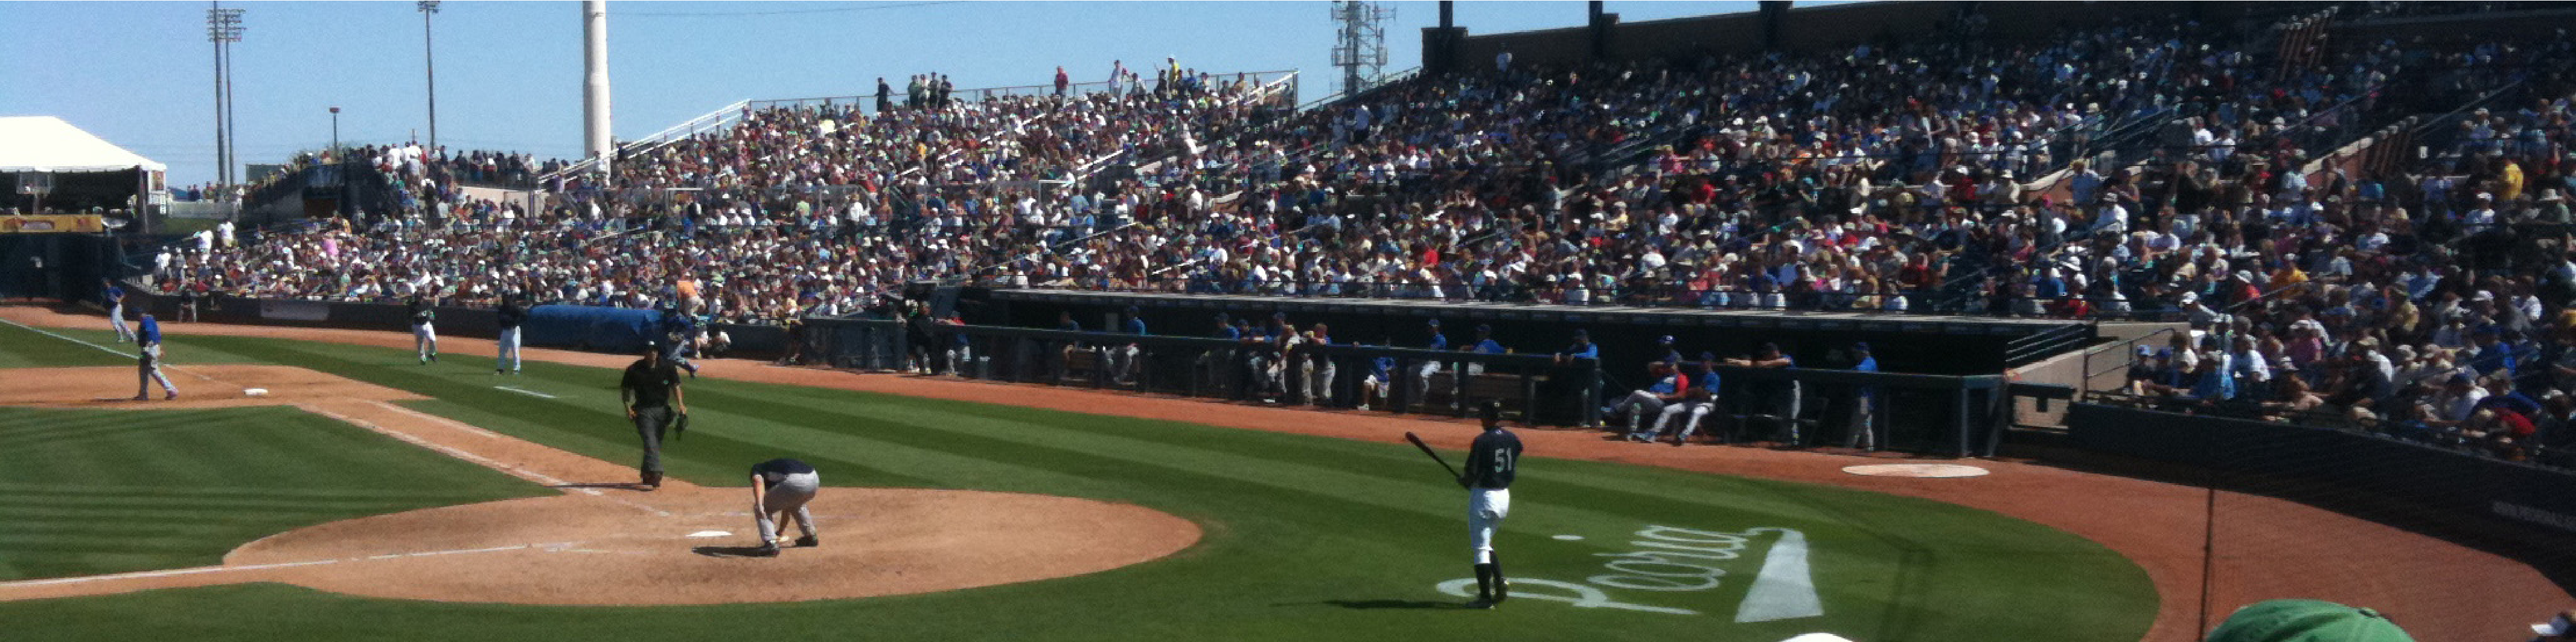
\includegraphics[width=\textwidth]{sampleteaser}
%   \caption{Seattle Mariners at Spring Training, 2010.}
%   \Description{Enjoying the baseball game from the third-base
%     seats. Ichiro Suzuki preparing to bat.}
%   \label{fig:teaser}
% \end{teaserfigure}

%%
%% This command processes the author and affiliation and title
%% information and builds the first part of the formatted document.
\maketitle

\section{Introduction} % Open

The adversarial robustness of GNNs has been widely studied in recent research beginning with~\citep{Zugner2018, Dai2018}. However, most previous work largely focused on graphs with less than 20,000 nodes. In particular, from the perspective of real-world internet-scale applications, those graphs are tiny. To attack a small dataset such as PubMed (19,717 nodes)~\citep{Sen2008}, typically around 20~GB is required if using a dense adjacency matrix. We argue that such memory requirements are impractical, hinder practitioners to assess adversarial robustness, and limit advancements of the field. In this work, we set the foundation for the holistic study of adversarial robustness of GNNs on real-world social/citation networks. 
We study graphs with up to 111 million nodes and therefore assess the adversarial robustness of GNNs on graphs 500 times larger than before. In Fig.~\ref{fig:memorycomparison}, we compare the memory requirements of a previous attack with ours for attacking a GNN globally (i.e.\ aiming for a reduced accuracy). Analogously to our attacks, we can scale our defense also to graphs with 111 million nodes and beyond.

%%%%%%%%%%%%%%%%%%%%%%%%%%%%%%%%%%%%%%%%%%%%%%%%%%%%%%%%%

\begin{figure}[h]
  \centering
  \resizebox{0.8\linewidth}{!}{%% Creator: Matplotlib, PGF backend
%%
%% To include the figure in your LaTeX document, write
%%   \input{<filename>.pgf}
%%
%% Make sure the required packages are loaded in your preamble
%%   \usepackage{pgf}
%%
%% and, on pdftex
%%   \usepackage[utf8]{inputenc}\DeclareUnicodeCharacter{2212}{-}
%%
%% or, on luatex and xetex
%%   \usepackage{unicode-math}
%%
%% Figures using additional raster images can only be included by \input if
%% they are in the same directory as the main LaTeX file. For loading figures
%% from other directories you can use the `import` package
%%   \usepackage{import}
%%
%% and then include the figures with
%%   \import{<path to file>}{<filename>.pgf}
%%
%% Matplotlib used the following preamble
%%   \usepackage[utf8]{inputenc}
%%   \usepackage[T1]{fontenc}
%%   \usepackage{amsmath}
%%   \newcommand*{\mat}[1]{\boldsymbol{#1}}
%%
\begingroup%
\makeatletter%
\begin{pgfpicture}%
\pgfpathrectangle{\pgfpointorigin}{\pgfqpoint{3.356466in}{1.938674in}}%
\pgfusepath{use as bounding box, clip}%
\begin{pgfscope}%
\pgfsetbuttcap%
\pgfsetmiterjoin%
\definecolor{currentfill}{rgb}{1.000000,1.000000,1.000000}%
\pgfsetfillcolor{currentfill}%
\pgfsetlinewidth{0.000000pt}%
\definecolor{currentstroke}{rgb}{1.000000,1.000000,1.000000}%
\pgfsetstrokecolor{currentstroke}%
\pgfsetstrokeopacity{0.000000}%
\pgfsetdash{}{0pt}%
\pgfpathmoveto{\pgfqpoint{0.000000in}{0.000000in}}%
\pgfpathlineto{\pgfqpoint{3.356466in}{0.000000in}}%
\pgfpathlineto{\pgfqpoint{3.356466in}{1.938674in}}%
\pgfpathlineto{\pgfqpoint{0.000000in}{1.938674in}}%
\pgfpathclose%
\pgfusepath{fill}%
\end{pgfscope}%
\begin{pgfscope}%
\pgfsetbuttcap%
\pgfsetmiterjoin%
\definecolor{currentfill}{rgb}{1.000000,1.000000,1.000000}%
\pgfsetfillcolor{currentfill}%
\pgfsetlinewidth{0.000000pt}%
\definecolor{currentstroke}{rgb}{0.000000,0.000000,0.000000}%
\pgfsetstrokecolor{currentstroke}%
\pgfsetstrokeopacity{0.000000}%
\pgfsetdash{}{0pt}%
\pgfpathmoveto{\pgfqpoint{0.544622in}{0.468349in}}%
\pgfpathlineto{\pgfqpoint{2.888997in}{0.468349in}}%
\pgfpathlineto{\pgfqpoint{2.888997in}{1.838674in}}%
\pgfpathlineto{\pgfqpoint{0.544622in}{1.838674in}}%
\pgfpathclose%
\pgfusepath{fill}%
\end{pgfscope}%
\begin{pgfscope}%
\pgfpathrectangle{\pgfqpoint{0.544622in}{0.468349in}}{\pgfqpoint{2.344375in}{1.370325in}}%
\pgfusepath{clip}%
\pgfsetroundcap%
\pgfsetroundjoin%
\pgfsetlinewidth{0.501875pt}%
\definecolor{currentstroke}{rgb}{0.800000,0.800000,0.800000}%
\pgfsetstrokecolor{currentstroke}%
\pgfsetdash{}{0pt}%
\pgfpathmoveto{\pgfqpoint{0.651185in}{0.468349in}}%
\pgfpathlineto{\pgfqpoint{0.651185in}{1.838674in}}%
\pgfusepath{stroke}%
\end{pgfscope}%
\begin{pgfscope}%
\definecolor{textcolor}{rgb}{0.150000,0.150000,0.150000}%
\pgfsetstrokecolor{textcolor}%
\pgfsetfillcolor{textcolor}%
\pgftext[x=0.651185in,y=0.378072in,,top]{\color{textcolor}\rmfamily\fontsize{8.000000}{9.600000}\selectfont \(\displaystyle {10^{3}}\)}%
\end{pgfscope}%
\begin{pgfscope}%
\pgfpathrectangle{\pgfqpoint{0.544622in}{0.468349in}}{\pgfqpoint{2.344375in}{1.370325in}}%
\pgfusepath{clip}%
\pgfsetroundcap%
\pgfsetroundjoin%
\pgfsetlinewidth{0.501875pt}%
\definecolor{currentstroke}{rgb}{0.800000,0.800000,0.800000}%
\pgfsetstrokecolor{currentstroke}%
\pgfsetdash{}{0pt}%
\pgfpathmoveto{\pgfqpoint{1.069698in}{0.468349in}}%
\pgfpathlineto{\pgfqpoint{1.069698in}{1.838674in}}%
\pgfusepath{stroke}%
\end{pgfscope}%
\begin{pgfscope}%
\definecolor{textcolor}{rgb}{0.150000,0.150000,0.150000}%
\pgfsetstrokecolor{textcolor}%
\pgfsetfillcolor{textcolor}%
\pgftext[x=1.069698in,y=0.378072in,,top]{\color{textcolor}\rmfamily\fontsize{8.000000}{9.600000}\selectfont \(\displaystyle {10^{4}}\)}%
\end{pgfscope}%
\begin{pgfscope}%
\pgfpathrectangle{\pgfqpoint{0.544622in}{0.468349in}}{\pgfqpoint{2.344375in}{1.370325in}}%
\pgfusepath{clip}%
\pgfsetroundcap%
\pgfsetroundjoin%
\pgfsetlinewidth{0.501875pt}%
\definecolor{currentstroke}{rgb}{0.800000,0.800000,0.800000}%
\pgfsetstrokecolor{currentstroke}%
\pgfsetdash{}{0pt}%
\pgfpathmoveto{\pgfqpoint{1.488211in}{0.468349in}}%
\pgfpathlineto{\pgfqpoint{1.488211in}{1.838674in}}%
\pgfusepath{stroke}%
\end{pgfscope}%
\begin{pgfscope}%
\definecolor{textcolor}{rgb}{0.150000,0.150000,0.150000}%
\pgfsetstrokecolor{textcolor}%
\pgfsetfillcolor{textcolor}%
\pgftext[x=1.488211in,y=0.378072in,,top]{\color{textcolor}\rmfamily\fontsize{8.000000}{9.600000}\selectfont \(\displaystyle {10^{5}}\)}%
\end{pgfscope}%
\begin{pgfscope}%
\pgfpathrectangle{\pgfqpoint{0.544622in}{0.468349in}}{\pgfqpoint{2.344375in}{1.370325in}}%
\pgfusepath{clip}%
\pgfsetroundcap%
\pgfsetroundjoin%
\pgfsetlinewidth{0.501875pt}%
\definecolor{currentstroke}{rgb}{0.800000,0.800000,0.800000}%
\pgfsetstrokecolor{currentstroke}%
\pgfsetdash{}{0pt}%
\pgfpathmoveto{\pgfqpoint{1.906724in}{0.468349in}}%
\pgfpathlineto{\pgfqpoint{1.906724in}{1.838674in}}%
\pgfusepath{stroke}%
\end{pgfscope}%
\begin{pgfscope}%
\definecolor{textcolor}{rgb}{0.150000,0.150000,0.150000}%
\pgfsetstrokecolor{textcolor}%
\pgfsetfillcolor{textcolor}%
\pgftext[x=1.906724in,y=0.378072in,,top]{\color{textcolor}\rmfamily\fontsize{8.000000}{9.600000}\selectfont \(\displaystyle {10^{6}}\)}%
\end{pgfscope}%
\begin{pgfscope}%
\pgfpathrectangle{\pgfqpoint{0.544622in}{0.468349in}}{\pgfqpoint{2.344375in}{1.370325in}}%
\pgfusepath{clip}%
\pgfsetroundcap%
\pgfsetroundjoin%
\pgfsetlinewidth{0.501875pt}%
\definecolor{currentstroke}{rgb}{0.800000,0.800000,0.800000}%
\pgfsetstrokecolor{currentstroke}%
\pgfsetdash{}{0pt}%
\pgfpathmoveto{\pgfqpoint{2.325237in}{0.468349in}}%
\pgfpathlineto{\pgfqpoint{2.325237in}{1.838674in}}%
\pgfusepath{stroke}%
\end{pgfscope}%
\begin{pgfscope}%
\definecolor{textcolor}{rgb}{0.150000,0.150000,0.150000}%
\pgfsetstrokecolor{textcolor}%
\pgfsetfillcolor{textcolor}%
\pgftext[x=2.325237in,y=0.378072in,,top]{\color{textcolor}\rmfamily\fontsize{8.000000}{9.600000}\selectfont \(\displaystyle {10^{7}}\)}%
\end{pgfscope}%
\begin{pgfscope}%
\pgfpathrectangle{\pgfqpoint{0.544622in}{0.468349in}}{\pgfqpoint{2.344375in}{1.370325in}}%
\pgfusepath{clip}%
\pgfsetroundcap%
\pgfsetroundjoin%
\pgfsetlinewidth{0.501875pt}%
\definecolor{currentstroke}{rgb}{0.800000,0.800000,0.800000}%
\pgfsetstrokecolor{currentstroke}%
\pgfsetdash{}{0pt}%
\pgfpathmoveto{\pgfqpoint{2.743750in}{0.468349in}}%
\pgfpathlineto{\pgfqpoint{2.743750in}{1.838674in}}%
\pgfusepath{stroke}%
\end{pgfscope}%
\begin{pgfscope}%
\definecolor{textcolor}{rgb}{0.150000,0.150000,0.150000}%
\pgfsetstrokecolor{textcolor}%
\pgfsetfillcolor{textcolor}%
\pgftext[x=2.743750in,y=0.378072in,,top]{\color{textcolor}\rmfamily\fontsize{8.000000}{9.600000}\selectfont \(\displaystyle {10^{8}}\)}%
\end{pgfscope}%
\begin{pgfscope}%
\definecolor{textcolor}{rgb}{0.150000,0.150000,0.150000}%
\pgfsetstrokecolor{textcolor}%
\pgfsetfillcolor{textcolor}%
\pgftext[x=1.716810in,y=0.222655in,,top]{\color{textcolor}\rmfamily\fontsize{10.000000}{12.000000}\selectfont \#Edges \(\displaystyle e\)}%
\end{pgfscope}%
\begin{pgfscope}%
\pgfpathrectangle{\pgfqpoint{0.544622in}{0.468349in}}{\pgfqpoint{2.344375in}{1.370325in}}%
\pgfusepath{clip}%
\pgfsetroundcap%
\pgfsetroundjoin%
\pgfsetlinewidth{0.501875pt}%
\definecolor{currentstroke}{rgb}{0.800000,0.800000,0.800000}%
\pgfsetstrokecolor{currentstroke}%
\pgfsetdash{}{0pt}%
\pgfpathmoveto{\pgfqpoint{0.544622in}{0.548666in}}%
\pgfpathlineto{\pgfqpoint{2.888997in}{0.548666in}}%
\pgfusepath{stroke}%
\end{pgfscope}%
\begin{pgfscope}%
\definecolor{textcolor}{rgb}{0.150000,0.150000,0.150000}%
\pgfsetstrokecolor{textcolor}%
\pgfsetfillcolor{textcolor}%
\pgftext[x=0.278211in, y=0.510403in, left, base]{\color{textcolor}\rmfamily\fontsize{8.000000}{9.600000}\selectfont GB}%
\end{pgfscope}%
\begin{pgfscope}%
\pgfpathrectangle{\pgfqpoint{0.544622in}{0.468349in}}{\pgfqpoint{2.344375in}{1.370325in}}%
\pgfusepath{clip}%
\pgfsetroundcap%
\pgfsetroundjoin%
\pgfsetlinewidth{0.501875pt}%
\definecolor{currentstroke}{rgb}{0.800000,0.800000,0.800000}%
\pgfsetstrokecolor{currentstroke}%
\pgfsetdash{}{0pt}%
\pgfpathmoveto{\pgfqpoint{0.544622in}{1.037410in}}%
\pgfpathlineto{\pgfqpoint{2.888997in}{1.037410in}}%
\pgfusepath{stroke}%
\end{pgfscope}%
\begin{pgfscope}%
\definecolor{textcolor}{rgb}{0.150000,0.150000,0.150000}%
\pgfsetstrokecolor{textcolor}%
\pgfsetfillcolor{textcolor}%
\pgftext[x=0.285558in, y=0.999148in, left, base]{\color{textcolor}\rmfamily\fontsize{8.000000}{9.600000}\selectfont TB}%
\end{pgfscope}%
\begin{pgfscope}%
\pgfpathrectangle{\pgfqpoint{0.544622in}{0.468349in}}{\pgfqpoint{2.344375in}{1.370325in}}%
\pgfusepath{clip}%
\pgfsetroundcap%
\pgfsetroundjoin%
\pgfsetlinewidth{0.501875pt}%
\definecolor{currentstroke}{rgb}{0.800000,0.800000,0.800000}%
\pgfsetstrokecolor{currentstroke}%
\pgfsetdash{}{0pt}%
\pgfpathmoveto{\pgfqpoint{0.544622in}{1.526154in}}%
\pgfpathlineto{\pgfqpoint{2.888997in}{1.526154in}}%
\pgfusepath{stroke}%
\end{pgfscope}%
\begin{pgfscope}%
\definecolor{textcolor}{rgb}{0.150000,0.150000,0.150000}%
\pgfsetstrokecolor{textcolor}%
\pgfsetfillcolor{textcolor}%
\pgftext[x=0.290534in, y=1.487892in, left, base]{\color{textcolor}\rmfamily\fontsize{8.000000}{9.600000}\selectfont PB}%
\end{pgfscope}%
\begin{pgfscope}%
\definecolor{textcolor}{rgb}{0.150000,0.150000,0.150000}%
\pgfsetstrokecolor{textcolor}%
\pgfsetfillcolor{textcolor}%
\pgftext[x=0.222655in,y=1.153512in,,bottom,rotate=90.000000]{\color{textcolor}\rmfamily\fontsize{10.000000}{12.000000}\selectfont Memory}%
\end{pgfscope}%
\begin{pgfscope}%
\pgfpathrectangle{\pgfqpoint{0.544622in}{0.468349in}}{\pgfqpoint{2.344375in}{1.370325in}}%
\pgfusepath{clip}%
\pgfsetroundcap%
\pgfsetroundjoin%
\pgfsetlinewidth{1.003750pt}%
\definecolor{currentstroke}{rgb}{0.100000,0.100000,0.100000}%
\pgfsetstrokecolor{currentstroke}%
\pgfsetdash{}{0pt}%
\pgfpathmoveto{\pgfqpoint{0.544622in}{0.793877in}}%
\pgfpathlineto{\pgfqpoint{2.888997in}{0.793877in}}%
\pgfusepath{stroke}%
\end{pgfscope}%
\begin{pgfscope}%
\pgfpathrectangle{\pgfqpoint{0.544622in}{0.468349in}}{\pgfqpoint{2.344375in}{1.370325in}}%
\pgfusepath{clip}%
\pgfsetbuttcap%
\pgfsetroundjoin%
\pgfsetlinewidth{1.003750pt}%
\definecolor{currentstroke}{rgb}{0.333333,0.658824,0.407843}%
\pgfsetstrokecolor{currentstroke}%
\pgfsetdash{{3.700000pt}{1.600000pt}}{0.000000pt}%
\pgfpathmoveto{\pgfqpoint{0.651185in}{0.530637in}}%
\pgfpathlineto{\pgfqpoint{0.715250in}{0.531665in}}%
\pgfpathlineto{\pgfqpoint{0.766503in}{0.532858in}}%
\pgfpathlineto{\pgfqpoint{0.809213in}{0.534215in}}%
\pgfpathlineto{\pgfqpoint{0.847653in}{0.535824in}}%
\pgfpathlineto{\pgfqpoint{0.877550in}{0.537408in}}%
\pgfpathlineto{\pgfqpoint{0.907447in}{0.539360in}}%
\pgfpathlineto{\pgfqpoint{0.933073in}{0.541392in}}%
\pgfpathlineto{\pgfqpoint{0.958700in}{0.543823in}}%
\pgfpathlineto{\pgfqpoint{0.980055in}{0.546209in}}%
\pgfpathlineto{\pgfqpoint{1.001410in}{0.548972in}}%
\pgfpathlineto{\pgfqpoint{1.022765in}{0.552167in}}%
\pgfpathlineto{\pgfqpoint{1.039850in}{0.555069in}}%
\pgfpathlineto{\pgfqpoint{1.056934in}{0.558311in}}%
\pgfpathlineto{\pgfqpoint{1.074018in}{0.561922in}}%
\pgfpathlineto{\pgfqpoint{1.091102in}{0.565930in}}%
\pgfpathlineto{\pgfqpoint{1.108186in}{0.570360in}}%
\pgfpathlineto{\pgfqpoint{1.125270in}{0.575238in}}%
\pgfpathlineto{\pgfqpoint{1.142355in}{0.580581in}}%
\pgfpathlineto{\pgfqpoint{1.159439in}{0.586406in}}%
\pgfpathlineto{\pgfqpoint{1.176523in}{0.592722in}}%
\pgfpathlineto{\pgfqpoint{1.193607in}{0.599533in}}%
\pgfpathlineto{\pgfqpoint{1.210691in}{0.606838in}}%
\pgfpathlineto{\pgfqpoint{1.227775in}{0.614628in}}%
\pgfpathlineto{\pgfqpoint{1.244860in}{0.622890in}}%
\pgfpathlineto{\pgfqpoint{1.261944in}{0.631606in}}%
\pgfpathlineto{\pgfqpoint{1.279028in}{0.640754in}}%
\pgfpathlineto{\pgfqpoint{1.296112in}{0.650308in}}%
\pgfpathlineto{\pgfqpoint{1.313196in}{0.660240in}}%
\pgfpathlineto{\pgfqpoint{1.334551in}{0.673145in}}%
\pgfpathlineto{\pgfqpoint{1.355907in}{0.686540in}}%
\pgfpathlineto{\pgfqpoint{1.377262in}{0.700369in}}%
\pgfpathlineto{\pgfqpoint{1.402888in}{0.717465in}}%
\pgfpathlineto{\pgfqpoint{1.428514in}{0.735028in}}%
\pgfpathlineto{\pgfqpoint{1.458412in}{0.756009in}}%
\pgfpathlineto{\pgfqpoint{1.492580in}{0.780514in}}%
\pgfpathlineto{\pgfqpoint{1.531019in}{0.808609in}}%
\pgfpathlineto{\pgfqpoint{1.573730in}{0.840319in}}%
\pgfpathlineto{\pgfqpoint{1.624982in}{0.878871in}}%
\pgfpathlineto{\pgfqpoint{1.684777in}{0.924326in}}%
\pgfpathlineto{\pgfqpoint{1.761656in}{0.983262in}}%
\pgfpathlineto{\pgfqpoint{1.864161in}{1.062353in}}%
\pgfpathlineto{\pgfqpoint{2.009376in}{1.174914in}}%
\pgfpathlineto{\pgfqpoint{2.248554in}{1.360837in}}%
\pgfpathlineto{\pgfqpoint{2.782435in}{1.776387in}}%
\pgfpathlineto{\pgfqpoint{2.782435in}{1.776387in}}%
\pgfusepath{stroke}%
\end{pgfscope}%
\begin{pgfscope}%
\pgfsetrectcap%
\pgfsetmiterjoin%
\pgfsetlinewidth{0.752812pt}%
\definecolor{currentstroke}{rgb}{0.700000,0.700000,0.700000}%
\pgfsetstrokecolor{currentstroke}%
\pgfsetdash{}{0pt}%
\pgfpathmoveto{\pgfqpoint{0.544622in}{0.468349in}}%
\pgfpathlineto{\pgfqpoint{0.544622in}{1.838674in}}%
\pgfusepath{stroke}%
\end{pgfscope}%
\begin{pgfscope}%
\pgfsetrectcap%
\pgfsetmiterjoin%
\pgfsetlinewidth{0.752812pt}%
\definecolor{currentstroke}{rgb}{0.700000,0.700000,0.700000}%
\pgfsetstrokecolor{currentstroke}%
\pgfsetdash{}{0pt}%
\pgfpathmoveto{\pgfqpoint{2.888997in}{0.468349in}}%
\pgfpathlineto{\pgfqpoint{2.888997in}{1.838674in}}%
\pgfusepath{stroke}%
\end{pgfscope}%
\begin{pgfscope}%
\pgfsetrectcap%
\pgfsetmiterjoin%
\pgfsetlinewidth{0.752812pt}%
\definecolor{currentstroke}{rgb}{0.700000,0.700000,0.700000}%
\pgfsetstrokecolor{currentstroke}%
\pgfsetdash{}{0pt}%
\pgfpathmoveto{\pgfqpoint{0.544622in}{0.468349in}}%
\pgfpathlineto{\pgfqpoint{2.888997in}{0.468349in}}%
\pgfusepath{stroke}%
\end{pgfscope}%
\begin{pgfscope}%
\pgfsetrectcap%
\pgfsetmiterjoin%
\pgfsetlinewidth{0.752812pt}%
\definecolor{currentstroke}{rgb}{0.700000,0.700000,0.700000}%
\pgfsetstrokecolor{currentstroke}%
\pgfsetdash{}{0pt}%
\pgfpathmoveto{\pgfqpoint{0.544622in}{1.838674in}}%
\pgfpathlineto{\pgfqpoint{2.888997in}{1.838674in}}%
\pgfusepath{stroke}%
\end{pgfscope}%
\begin{pgfscope}%
\pgfpathrectangle{\pgfqpoint{0.544622in}{0.468349in}}{\pgfqpoint{2.344375in}{1.370325in}}%
\pgfusepath{clip}%
\pgfsetbuttcap%
\pgfsetroundjoin%
\definecolor{currentfill}{rgb}{0.298039,0.447059,0.690196}%
\pgfsetfillcolor{currentfill}%
\pgfsetlinewidth{1.003750pt}%
\definecolor{currentstroke}{rgb}{0.298039,0.447059,0.690196}%
\pgfsetstrokecolor{currentstroke}%
\pgfsetdash{}{0pt}%
\pgfsys@defobject{currentmarker}{\pgfqpoint{-0.041667in}{-0.041667in}}{\pgfqpoint{0.041667in}{0.041667in}}{%
\pgfpathmoveto{\pgfqpoint{0.000000in}{-0.041667in}}%
\pgfpathcurveto{\pgfqpoint{0.011050in}{-0.041667in}}{\pgfqpoint{0.021649in}{-0.037276in}}{\pgfqpoint{0.029463in}{-0.029463in}}%
\pgfpathcurveto{\pgfqpoint{0.037276in}{-0.021649in}}{\pgfqpoint{0.041667in}{-0.011050in}}{\pgfqpoint{0.041667in}{0.000000in}}%
\pgfpathcurveto{\pgfqpoint{0.041667in}{0.011050in}}{\pgfqpoint{0.037276in}{0.021649in}}{\pgfqpoint{0.029463in}{0.029463in}}%
\pgfpathcurveto{\pgfqpoint{0.021649in}{0.037276in}}{\pgfqpoint{0.011050in}{0.041667in}}{\pgfqpoint{0.000000in}{0.041667in}}%
\pgfpathcurveto{\pgfqpoint{-0.011050in}{0.041667in}}{\pgfqpoint{-0.021649in}{0.037276in}}{\pgfqpoint{-0.029463in}{0.029463in}}%
\pgfpathcurveto{\pgfqpoint{-0.037276in}{0.021649in}}{\pgfqpoint{-0.041667in}{0.011050in}}{\pgfqpoint{-0.041667in}{0.000000in}}%
\pgfpathcurveto{\pgfqpoint{-0.041667in}{-0.011050in}}{\pgfqpoint{-0.037276in}{-0.021649in}}{\pgfqpoint{-0.029463in}{-0.029463in}}%
\pgfpathcurveto{\pgfqpoint{-0.021649in}{-0.037276in}}{\pgfqpoint{-0.011050in}{-0.041667in}}{\pgfqpoint{0.000000in}{-0.041667in}}%
\pgfpathclose%
\pgfusepath{stroke,fill}%
}%
\begin{pgfscope}%
\pgfsys@transformshift{1.013391in}{0.550708in}%
\pgfsys@useobject{currentmarker}{}%
\end{pgfscope}%
\begin{pgfscope}%
\pgfsys@transformshift{1.154692in}{0.584739in}%
\pgfsys@useobject{currentmarker}{}%
\end{pgfscope}%
\begin{pgfscope}%
\pgfsys@transformshift{1.466310in}{0.761628in}%
\pgfsys@useobject{currentmarker}{}%
\end{pgfscope}%
\end{pgfscope}%
\begin{pgfscope}%
\pgfpathrectangle{\pgfqpoint{0.544622in}{0.468349in}}{\pgfqpoint{2.344375in}{1.370325in}}%
\pgfusepath{clip}%
\pgfsetbuttcap%
\pgfsetmiterjoin%
\definecolor{currentfill}{rgb}{0.866667,0.517647,0.321569}%
\pgfsetfillcolor{currentfill}%
\pgfsetlinewidth{1.003750pt}%
\definecolor{currentstroke}{rgb}{0.866667,0.517647,0.321569}%
\pgfsetstrokecolor{currentstroke}%
\pgfsetdash{}{0pt}%
\pgfsys@defobject{currentmarker}{\pgfqpoint{-0.041667in}{-0.041667in}}{\pgfqpoint{0.041667in}{0.041667in}}{%
\pgfpathmoveto{\pgfqpoint{-0.020833in}{-0.041667in}}%
\pgfpathlineto{\pgfqpoint{0.000000in}{-0.020833in}}%
\pgfpathlineto{\pgfqpoint{0.020833in}{-0.041667in}}%
\pgfpathlineto{\pgfqpoint{0.041667in}{-0.020833in}}%
\pgfpathlineto{\pgfqpoint{0.020833in}{0.000000in}}%
\pgfpathlineto{\pgfqpoint{0.041667in}{0.020833in}}%
\pgfpathlineto{\pgfqpoint{0.020833in}{0.041667in}}%
\pgfpathlineto{\pgfqpoint{0.000000in}{0.020833in}}%
\pgfpathlineto{\pgfqpoint{-0.020833in}{0.041667in}}%
\pgfpathlineto{\pgfqpoint{-0.041667in}{0.020833in}}%
\pgfpathlineto{\pgfqpoint{-0.020833in}{0.000000in}}%
\pgfpathlineto{\pgfqpoint{-0.041667in}{-0.020833in}}%
\pgfpathclose%
\pgfusepath{stroke,fill}%
}%
\begin{pgfscope}%
\pgfsys@transformshift{1.013391in}{0.543332in}%
\pgfsys@useobject{currentmarker}{}%
\end{pgfscope}%
\begin{pgfscope}%
\pgfsys@transformshift{1.154692in}{0.565736in}%
\pgfsys@useobject{currentmarker}{}%
\end{pgfscope}%
\begin{pgfscope}%
\pgfsys@transformshift{1.466310in}{0.679830in}%
\pgfsys@useobject{currentmarker}{}%
\end{pgfscope}%
\begin{pgfscope}%
\pgfsys@transformshift{1.934676in}{0.701719in}%
\pgfsys@useobject{currentmarker}{}%
\end{pgfscope}%
\begin{pgfscope}%
\pgfsys@transformshift{2.782435in}{0.783465in}%
\pgfsys@useobject{currentmarker}{}%
\end{pgfscope}%
\end{pgfscope}%
\begin{pgfscope}%
\definecolor{textcolor}{rgb}{0.150000,0.150000,0.150000}%
\pgfsetstrokecolor{textcolor}%
\pgfsetfillcolor{textcolor}%
\pgftext[x=2.910293in,y=0.791630in,left,]{\color{textcolor}\rmfamily\fontsize{10.000000}{12.000000}\selectfont 32GB}%
\end{pgfscope}%
\begin{pgfscope}%
\definecolor{textcolor}{rgb}{0.150000,0.150000,0.150000}%
\pgfsetstrokecolor{textcolor}%
\pgfsetfillcolor{textcolor}%
\pgftext[x=2.870386in,y=0.686345in,right,]{\color{textcolor}\rmfamily\fontsize{10.000000}{12.000000}\selectfont Products}%
\end{pgfscope}%
\begin{pgfscope}%
\definecolor{textcolor}{rgb}{0.150000,0.150000,0.150000}%
\pgfsetstrokecolor{textcolor}%
\pgfsetfillcolor{textcolor}%
\pgftext[x=1.934676in,y=0.597708in,,]{\color{textcolor}\rmfamily\fontsize{10.000000}{12.000000}\selectfont arXiv}%
\end{pgfscope}%
\begin{pgfscope}%
\pgfsetbuttcap%
\pgfsetmiterjoin%
\definecolor{currentfill}{rgb}{1.000000,1.000000,1.000000}%
\pgfsetfillcolor{currentfill}%
\pgfsetfillopacity{0.800000}%
\pgfsetlinewidth{1.003750pt}%
\definecolor{currentstroke}{rgb}{0.800000,0.800000,0.800000}%
\pgfsetstrokecolor{currentstroke}%
\pgfsetstrokeopacity{0.800000}%
\pgfsetdash{}{0pt}%
\pgfpathmoveto{\pgfqpoint{0.622400in}{1.118347in}}%
\pgfpathlineto{\pgfqpoint{1.791549in}{1.118347in}}%
\pgfpathquadraticcurveto{\pgfqpoint{1.813772in}{1.118347in}}{\pgfqpoint{1.813772in}{1.140569in}}%
\pgfpathlineto{\pgfqpoint{1.813772in}{1.760897in}}%
\pgfpathquadraticcurveto{\pgfqpoint{1.813772in}{1.783119in}}{\pgfqpoint{1.791549in}{1.783119in}}%
\pgfpathlineto{\pgfqpoint{0.622400in}{1.783119in}}%
\pgfpathquadraticcurveto{\pgfqpoint{0.600178in}{1.783119in}}{\pgfqpoint{0.600178in}{1.760897in}}%
\pgfpathlineto{\pgfqpoint{0.600178in}{1.140569in}}%
\pgfpathquadraticcurveto{\pgfqpoint{0.600178in}{1.118347in}}{\pgfqpoint{0.622400in}{1.118347in}}%
\pgfpathclose%
\pgfusepath{stroke,fill}%
\end{pgfscope}%
\begin{pgfscope}%
\pgfsetbuttcap%
\pgfsetroundjoin%
\definecolor{currentfill}{rgb}{0.298039,0.447059,0.690196}%
\pgfsetfillcolor{currentfill}%
\pgfsetlinewidth{1.003750pt}%
\definecolor{currentstroke}{rgb}{0.298039,0.447059,0.690196}%
\pgfsetstrokecolor{currentstroke}%
\pgfsetdash{}{0pt}%
\pgfsys@defobject{currentmarker}{\pgfqpoint{-0.041667in}{-0.041667in}}{\pgfqpoint{0.041667in}{0.041667in}}{%
\pgfpathmoveto{\pgfqpoint{0.000000in}{-0.041667in}}%
\pgfpathcurveto{\pgfqpoint{0.011050in}{-0.041667in}}{\pgfqpoint{0.021649in}{-0.037276in}}{\pgfqpoint{0.029463in}{-0.029463in}}%
\pgfpathcurveto{\pgfqpoint{0.037276in}{-0.021649in}}{\pgfqpoint{0.041667in}{-0.011050in}}{\pgfqpoint{0.041667in}{0.000000in}}%
\pgfpathcurveto{\pgfqpoint{0.041667in}{0.011050in}}{\pgfqpoint{0.037276in}{0.021649in}}{\pgfqpoint{0.029463in}{0.029463in}}%
\pgfpathcurveto{\pgfqpoint{0.021649in}{0.037276in}}{\pgfqpoint{0.011050in}{0.041667in}}{\pgfqpoint{0.000000in}{0.041667in}}%
\pgfpathcurveto{\pgfqpoint{-0.011050in}{0.041667in}}{\pgfqpoint{-0.021649in}{0.037276in}}{\pgfqpoint{-0.029463in}{0.029463in}}%
\pgfpathcurveto{\pgfqpoint{-0.037276in}{0.021649in}}{\pgfqpoint{-0.041667in}{0.011050in}}{\pgfqpoint{-0.041667in}{0.000000in}}%
\pgfpathcurveto{\pgfqpoint{-0.041667in}{-0.011050in}}{\pgfqpoint{-0.037276in}{-0.021649in}}{\pgfqpoint{-0.029463in}{-0.029463in}}%
\pgfpathcurveto{\pgfqpoint{-0.021649in}{-0.037276in}}{\pgfqpoint{-0.011050in}{-0.041667in}}{\pgfqpoint{0.000000in}{-0.041667in}}%
\pgfpathclose%
\pgfusepath{stroke,fill}%
}%
\begin{pgfscope}%
\pgfsys@transformshift{0.755733in}{1.699786in}%
\pgfsys@useobject{currentmarker}{}%
\end{pgfscope}%
\end{pgfscope}%
\begin{pgfscope}%
\definecolor{textcolor}{rgb}{0.150000,0.150000,0.150000}%
\pgfsetstrokecolor{textcolor}%
\pgfsetfillcolor{textcolor}%
\pgftext[x=0.955733in,y=1.660897in,left,base]{\color{textcolor}\rmfamily\fontsize{8.000000}{9.600000}\selectfont PGD}%
\end{pgfscope}%
\begin{pgfscope}%
\pgfsetbuttcap%
\pgfsetmiterjoin%
\definecolor{currentfill}{rgb}{0.866667,0.517647,0.321569}%
\pgfsetfillcolor{currentfill}%
\pgfsetlinewidth{1.003750pt}%
\definecolor{currentstroke}{rgb}{0.866667,0.517647,0.321569}%
\pgfsetstrokecolor{currentstroke}%
\pgfsetdash{}{0pt}%
\pgfsys@defobject{currentmarker}{\pgfqpoint{-0.041667in}{-0.041667in}}{\pgfqpoint{0.041667in}{0.041667in}}{%
\pgfpathmoveto{\pgfqpoint{-0.020833in}{-0.041667in}}%
\pgfpathlineto{\pgfqpoint{0.000000in}{-0.020833in}}%
\pgfpathlineto{\pgfqpoint{0.020833in}{-0.041667in}}%
\pgfpathlineto{\pgfqpoint{0.041667in}{-0.020833in}}%
\pgfpathlineto{\pgfqpoint{0.020833in}{0.000000in}}%
\pgfpathlineto{\pgfqpoint{0.041667in}{0.020833in}}%
\pgfpathlineto{\pgfqpoint{0.020833in}{0.041667in}}%
\pgfpathlineto{\pgfqpoint{0.000000in}{0.020833in}}%
\pgfpathlineto{\pgfqpoint{-0.020833in}{0.041667in}}%
\pgfpathlineto{\pgfqpoint{-0.041667in}{0.020833in}}%
\pgfpathlineto{\pgfqpoint{-0.020833in}{0.000000in}}%
\pgfpathlineto{\pgfqpoint{-0.041667in}{-0.020833in}}%
\pgfpathclose%
\pgfusepath{stroke,fill}%
}%
\begin{pgfscope}%
\pgfsys@transformshift{0.755733in}{1.539317in}%
\pgfsys@useobject{currentmarker}{}%
\end{pgfscope}%
\end{pgfscope}%
\begin{pgfscope}%
\definecolor{textcolor}{rgb}{0.150000,0.150000,0.150000}%
\pgfsetstrokecolor{textcolor}%
\pgfsetfillcolor{textcolor}%
\pgftext[x=0.955733in,y=1.500428in,left,base]{\color{textcolor}\rmfamily\fontsize{8.000000}{9.600000}\selectfont PR-BCD (ours)}%
\end{pgfscope}%
\begin{pgfscope}%
\pgfsetbuttcap%
\pgfsetroundjoin%
\pgfsetlinewidth{1.003750pt}%
\definecolor{currentstroke}{rgb}{0.333333,0.658824,0.407843}%
\pgfsetstrokecolor{currentstroke}%
\pgfsetdash{{3.700000pt}{1.600000pt}}{0.000000pt}%
\pgfpathmoveto{\pgfqpoint{0.644622in}{1.378213in}}%
\pgfpathlineto{\pgfqpoint{0.866844in}{1.378213in}}%
\pgfusepath{stroke}%
\end{pgfscope}%
\begin{pgfscope}%
\definecolor{textcolor}{rgb}{0.150000,0.150000,0.150000}%
\pgfsetstrokecolor{textcolor}%
\pgfsetfillcolor{textcolor}%
\pgftext[x=0.955733in,y=1.339324in,left,base]{\color{textcolor}\rmfamily\fontsize{8.000000}{9.600000}\selectfont PGD trend}%
\end{pgfscope}%
\begin{pgfscope}%
\pgfsetroundcap%
\pgfsetroundjoin%
\pgfsetlinewidth{1.003750pt}%
\definecolor{currentstroke}{rgb}{0.100000,0.100000,0.100000}%
\pgfsetstrokecolor{currentstroke}%
\pgfsetdash{}{0pt}%
\pgfpathmoveto{\pgfqpoint{0.644622in}{1.223280in}}%
\pgfpathlineto{\pgfqpoint{0.866844in}{1.223280in}}%
\pgfusepath{stroke}%
\end{pgfscope}%
\begin{pgfscope}%
\definecolor{textcolor}{rgb}{0.150000,0.150000,0.150000}%
\pgfsetstrokecolor{textcolor}%
\pgfsetfillcolor{textcolor}%
\pgftext[x=0.955733in,y=1.184391in,left,base]{\color{textcolor}\rmfamily\fontsize{8.000000}{9.600000}\selectfont Tesla V100}%
\end{pgfscope}%
\end{pgfpicture}%
\makeatother%
\endgroup%
}
  \caption{GPU memory consumption for a global attack with Projected Gradient Descent (PGD)~\citep{Xu2019a}, its quadratic extrapolation, and our Projected Randomized Block Coordinate Descent (PR-BCD) (Sec.~\ref{sec:prbcd}). 
  Both yield similar perturbed accuracy.
  Beyond attacks, our defense % relying on the differentiable Soft Median aggregation
  (Sec.~\ref{sec:defense}) can also be applied on such scales. Using a scalable GNN and a local attack we can scale attacks and defenses to even larger graphs. \label{fig:memorycomparison}}
\end{figure}

%%%%%%%%%%%%%%%%%%%%%%%%%%%%%%%%%%%%%%%%%%%%%%%%%%%%%%%%%

\textbf{Scope.} In this work, we focus on adversarial robustness w.r.t.\ structure perturbations of GNNs for node classification. The GNN \(f(\adj, \features)\) is applied to a Graph \(\gG=(\adj, \features)\) with adjacency matrix \(\adj\) and node attributes \(\features\).
%Nonetheless, our global attacks can be easily generalized to graph classification. 
We solely consider \emph{evasion} (test time) attacks, but our approach could also serve as a building block in scaling \emph{poisoning} (train time) attacks~\cite{Zugner2019a}. We distinguish between \emph{local} attacks on a single or small group of nodes and \emph{global} attacks that consider all or a large fraction of nodes with a shared global budget \(\Delta\) denoting the maximum number of adversarial perturbations. It is apparent that local attacks are much easier to scale than global attacks since for a local attack we only need to obtain the prediction for a few (or a single) nodes. We study an adversary with perfect knowledge about the graph, GNN, and test labels. Even this white-box scenario has not been studied for large graphs and our primary goal is to empirically assess worst-case adversarial robustness.

\textbf{Challenges.} We identify three major challenges hindering the study of GNNs' adversarial robustness at scale: (1) Previous losses are not well-suited for global attacks on GNNs at scale. (2) Attacks on GNNs typically come with quadratic space complexity. (3) Virtually no adversarial defense exists for large graphs. We tackle all three in this paper.

\textbf{Surrogate losses (1).} We study the limitation of state of the art surrogate losses for attacking the accuracy of a GNN over all nodes, following~\citep{Chen2018, Wu2019, Xu2018, Zugner2019a} (Sec.~\ref{sec:ceisbad}). Especially in combination with small/realistic budgets \(\Delta\) and on large graphs, previous surrogate losses lead to weak attacks. In particular, Cross Entropy (\(\text{CE}\)) or the widely used Carlini-Wagner loss~\citep{Carlini2017} are bad surrogates for such global attacks. Our novel losses that overcome these limitations easily improve the strength of the attack by 100\%. For larger datasets, we observe gains of more than 200\%. Are GNNs perhaps even more fragile than previously believed?

\textbf{Attacks (2).} Scaling attacks is non-trivial. Attacks based on combinatorial approaches easily become computationally infeasible because of the vast amount of potential adjacency matrices (\(\mathcal{O}(2^{n^2})\)).
We can approximate the resulting discrete combinatorial optimization problem using first-order optimization attacks. Such attacks typically require the gradient towards all entries of the adjacency matrix, reducing the complexity to \(\Theta(n^2)\) which is still not feasible for massive graphs. We propose two strategies to apply first-order optimization without the burden of a dense adjacency matrix. In Sec.~\ref{sec:prbcd}, we describe how to add/remove edges between existing nodes based on Randomized Block Coordinate Descent (R-BCD) at an additional memory requirement of \(\mathcal{O}(\Delta)\)\footnote{The method in Sec.~\ref{sec:prbcd} was partially discussed at a non-archival workshop~\citep{Anonymous2021}. For double-blind rules we do not disclose the author list.}. Due to the limited scalability of traditional GNNs, we also consider the case where we attack PPRGo \cite{Bojchevski2020a}, a scalable GNN. We even obtain an algorithm with constant complexity w.r.t.\ the graph size.

\textbf{Defense (3).} We propose \emph{Soft Median} -- a computationally less demanding, robust, differentiable aggregation function inspired by~\citet{Geisler2020}, by taking advantage of recent advancements in differentiable sorting~\cite{Prillo2020}. Using Soft Median we observe similar robustness to~\citep{Geisler2020}, but with a significantly lower memory footprint, which enables us to defend GNNs at scale.
% we can leverage the lower memory footprint in GNNs when memory is at premium, i.e.\ this aggregation is suitable for defending a GNN at scale.

\section{Surrogate Losses}\label{sec:ceisbad} % Simon

Most GNNs for node classification are soft classifiers and predict a probability or confidence score  \(\vp_i = f(\adj, \features)_i\) for node \(i\) instead of the discrete classes. During training, we ideally wish to optimize a target metric which comes with a discontinuous loss (e.g.\ accuracy and the 0/1 loss \(\mathcal{L}_{0/1}\)). We typically use gradient methods to optimize our models and therefore commonly substitute the actual target loss by a differentiable \emph{surrogate} \(\mathcal{L}' \approx \mathcal{L}\), e.g., cross entropy for the 0/1 loss. The same is true for attacking a model to assess its \emph{adversarial robustness}. In the context of images, typically a single example is attacked in isolation, which corresponds to a \emph{local} attack for GNNs. In such a scenario it is often sufficient for an untargeted attack to \textit{maximize} the cross entropy for the attacked node/image:
\begin{equation}\label{eq:crossentropy}
\text{CE}^{(n)}(y, \vp) = \sum_{c \in \sC} \mathbb{I}[y^{(n)} = c] \log(\evp_{c})^{(n)} = \log(\evp_{c^*}^{(n)})\,.
\end{equation}
which corresponds to a minimization of the likelihood of the target class \(c^*\). Many \emph{global} attacks for GNNs~\citep{Chen2018, Wu2019, Xu2018, Zugner2019a} maximize the cross entropy \(\max_{\adj} \text{CE}(f_{\theta}(\adj, \features))\) on the \emph{whole dataset}, subject to a global budget constraint \(\Delta\). However, especially on large graphs, we often observed that the \(\text{CE}\) loss increases even though the accuracy does not decline. This can be explained by a bias of \(\text{CE}\) towards nodes which have a low confidence score, i.e.\ with \(\text{CE}\) we primarily attack nodes that are already misclassified. In other word those points have already a negative classification margin \(\psi = \min_{c \ne c^*} \evp_{c^*} - \evp_{c}\) as we can see in Fig.~\ref{fig:negceprob}.

%%%%%%%%%%%%%%%%%%%%%%%%%%%%%%%%%%%%%%%%%%%%%%%%%%%%%%%%%%%%%%%%%%%%

\begin{figure}[t]
  \centering
  \resizebox{\linewidth}{!}{%% Creator: Matplotlib, PGF backend
%%
%% To include the figure in your LaTeX document, write
%%   \input{<filename>.pgf}
%%
%% Make sure the required packages are loaded in your preamble
%%   \usepackage{pgf}
%%
%% and, on pdftex
%%   \usepackage[utf8]{inputenc}\DeclareUnicodeCharacter{2212}{-}
%%
%% or, on luatex and xetex
%%   \usepackage{unicode-math}
%%
%% Figures using additional raster images can only be included by \input if
%% they are in the same directory as the main LaTeX file. For loading figures
%% from other directories you can use the `import` package
%%   \usepackage{import}
%%
%% and then include the figures with
%%   \import{<path to file>}{<filename>.pgf}
%%
%% Matplotlib used the following preamble
%%   \usepackage[utf8]{inputenc}
%%   \usepackage[T1]{fontenc}
%%   \usepackage{amsmath}
%%   \newcommand*{\mat}[1]{\boldsymbol{#1}}
%%
\begingroup%
\makeatletter%
\begin{pgfpicture}%
\pgfpathrectangle{\pgfpointorigin}{\pgfqpoint{4.774678in}{1.388808in}}%
\pgfusepath{use as bounding box, clip}%
\begin{pgfscope}%
\pgfsetbuttcap%
\pgfsetmiterjoin%
\definecolor{currentfill}{rgb}{1.000000,1.000000,1.000000}%
\pgfsetfillcolor{currentfill}%
\pgfsetlinewidth{0.000000pt}%
\definecolor{currentstroke}{rgb}{1.000000,1.000000,1.000000}%
\pgfsetstrokecolor{currentstroke}%
\pgfsetstrokeopacity{0.000000}%
\pgfsetdash{}{0pt}%
\pgfpathmoveto{\pgfqpoint{0.000000in}{0.000000in}}%
\pgfpathlineto{\pgfqpoint{4.774678in}{0.000000in}}%
\pgfpathlineto{\pgfqpoint{4.774678in}{1.388808in}}%
\pgfpathlineto{\pgfqpoint{0.000000in}{1.388808in}}%
\pgfpathclose%
\pgfusepath{fill}%
\end{pgfscope}%
\begin{pgfscope}%
\pgfsetbuttcap%
\pgfsetmiterjoin%
\definecolor{currentfill}{rgb}{1.000000,1.000000,1.000000}%
\pgfsetfillcolor{currentfill}%
\pgfsetlinewidth{0.000000pt}%
\definecolor{currentstroke}{rgb}{0.000000,0.000000,0.000000}%
\pgfsetstrokecolor{currentstroke}%
\pgfsetstrokeopacity{0.000000}%
\pgfsetdash{}{0pt}%
\pgfpathmoveto{\pgfqpoint{0.652433in}{0.466613in}}%
\pgfpathlineto{\pgfqpoint{3.209933in}{0.466613in}}%
\pgfpathlineto{\pgfqpoint{3.209933in}{1.288808in}}%
\pgfpathlineto{\pgfqpoint{0.652433in}{1.288808in}}%
\pgfpathclose%
\pgfusepath{fill}%
\end{pgfscope}%
\begin{pgfscope}%
\definecolor{textcolor}{rgb}{0.150000,0.150000,0.150000}%
\pgfsetstrokecolor{textcolor}%
\pgfsetfillcolor{textcolor}%
\pgftext[x=0.652433in,y=0.376335in,,top]{\color{textcolor}\rmfamily\fontsize{8.000000}{9.600000}\selectfont \(\displaystyle {0.0}\)}%
\end{pgfscope}%
\begin{pgfscope}%
\definecolor{textcolor}{rgb}{0.150000,0.150000,0.150000}%
\pgfsetstrokecolor{textcolor}%
\pgfsetfillcolor{textcolor}%
\pgftext[x=1.139576in,y=0.376335in,,top]{\color{textcolor}\rmfamily\fontsize{8.000000}{9.600000}\selectfont \(\displaystyle {0.2}\)}%
\end{pgfscope}%
\begin{pgfscope}%
\definecolor{textcolor}{rgb}{0.150000,0.150000,0.150000}%
\pgfsetstrokecolor{textcolor}%
\pgfsetfillcolor{textcolor}%
\pgftext[x=1.626719in,y=0.376335in,,top]{\color{textcolor}\rmfamily\fontsize{8.000000}{9.600000}\selectfont \(\displaystyle {0.4}\)}%
\end{pgfscope}%
\begin{pgfscope}%
\definecolor{textcolor}{rgb}{0.150000,0.150000,0.150000}%
\pgfsetstrokecolor{textcolor}%
\pgfsetfillcolor{textcolor}%
\pgftext[x=2.113862in,y=0.376335in,,top]{\color{textcolor}\rmfamily\fontsize{8.000000}{9.600000}\selectfont \(\displaystyle {0.6}\)}%
\end{pgfscope}%
\begin{pgfscope}%
\definecolor{textcolor}{rgb}{0.150000,0.150000,0.150000}%
\pgfsetstrokecolor{textcolor}%
\pgfsetfillcolor{textcolor}%
\pgftext[x=2.601005in,y=0.376335in,,top]{\color{textcolor}\rmfamily\fontsize{8.000000}{9.600000}\selectfont \(\displaystyle {0.8}\)}%
\end{pgfscope}%
\begin{pgfscope}%
\definecolor{textcolor}{rgb}{0.150000,0.150000,0.150000}%
\pgfsetstrokecolor{textcolor}%
\pgfsetfillcolor{textcolor}%
\pgftext[x=3.088148in,y=0.376335in,,top]{\color{textcolor}\rmfamily\fontsize{8.000000}{9.600000}\selectfont \(\displaystyle {1.0}\)}%
\end{pgfscope}%
\begin{pgfscope}%
\definecolor{textcolor}{rgb}{0.150000,0.150000,0.150000}%
\pgfsetstrokecolor{textcolor}%
\pgfsetfillcolor{textcolor}%
\pgftext[x=1.931183in,y=0.222655in,,top]{\color{textcolor}\rmfamily\fontsize{10.000000}{12.000000}\selectfont Frequency}%
\end{pgfscope}%
\begin{pgfscope}%
\definecolor{textcolor}{rgb}{0.150000,0.150000,0.150000}%
\pgfsetstrokecolor{textcolor}%
\pgfsetfillcolor{textcolor}%
\pgftext[x=0.408181in, y=1.155457in, left, base]{\color{textcolor}\rmfamily\fontsize{8.000000}{9.600000}\selectfont All}%
\end{pgfscope}%
\begin{pgfscope}%
\definecolor{textcolor}{rgb}{0.150000,0.150000,0.150000}%
\pgfsetstrokecolor{textcolor}%
\pgfsetfillcolor{textcolor}%
\pgftext[x=0.269712in, y=1.042027in, left, base]{\color{textcolor}\rmfamily\fontsize{8.000000}{9.600000}\selectfont nodes}%
\end{pgfscope}%
\begin{pgfscope}%
\definecolor{textcolor}{rgb}{0.150000,0.150000,0.150000}%
\pgfsetstrokecolor{textcolor}%
\pgfsetfillcolor{textcolor}%
\pgftext[x=0.100000in, y=0.621564in, left, base]{\color{textcolor}\rmfamily\fontsize{8.000000}{9.600000}\selectfont Attacked}%
\end{pgfscope}%
\begin{pgfscope}%
\definecolor{textcolor}{rgb}{0.150000,0.150000,0.150000}%
\pgfsetstrokecolor{textcolor}%
\pgfsetfillcolor{textcolor}%
\pgftext[x=0.269712in, y=0.508134in, left, base]{\color{textcolor}\rmfamily\fontsize{8.000000}{9.600000}\selectfont nodes}%
\end{pgfscope}%
\begin{pgfscope}%
\pgfpathrectangle{\pgfqpoint{0.652433in}{0.466613in}}{\pgfqpoint{2.557500in}{0.822195in}}%
\pgfusepath{clip}%
\pgfsetbuttcap%
\pgfsetmiterjoin%
\definecolor{currentfill}{rgb}{0.417086,0.680631,0.838231}%
\pgfsetfillcolor{currentfill}%
\pgfsetlinewidth{1.003750pt}%
\definecolor{currentstroke}{rgb}{1.000000,1.000000,1.000000}%
\pgfsetstrokecolor{currentstroke}%
\pgfsetdash{}{0pt}%
\pgfpathmoveto{\pgfqpoint{0.652433in}{1.037878in}}%
\pgfpathlineto{\pgfqpoint{3.088148in}{1.037878in}}%
\pgfpathlineto{\pgfqpoint{3.088148in}{1.251435in}}%
\pgfpathlineto{\pgfqpoint{0.652433in}{1.251435in}}%
\pgfpathclose%
\pgfusepath{stroke,fill}%
\end{pgfscope}%
\begin{pgfscope}%
\pgfpathrectangle{\pgfqpoint{0.652433in}{0.466613in}}{\pgfqpoint{2.557500in}{0.822195in}}%
\pgfusepath{clip}%
\pgfsetbuttcap%
\pgfsetmiterjoin%
\definecolor{currentfill}{rgb}{0.417086,0.680631,0.838231}%
\pgfsetfillcolor{currentfill}%
\pgfsetlinewidth{1.003750pt}%
\definecolor{currentstroke}{rgb}{1.000000,1.000000,1.000000}%
\pgfsetstrokecolor{currentstroke}%
\pgfsetdash{}{0pt}%
\pgfpathmoveto{\pgfqpoint{0.652433in}{0.503985in}}%
\pgfpathlineto{\pgfqpoint{3.088148in}{0.503985in}}%
\pgfpathlineto{\pgfqpoint{3.088148in}{0.717542in}}%
\pgfpathlineto{\pgfqpoint{0.652433in}{0.717542in}}%
\pgfpathclose%
\pgfusepath{stroke,fill}%
\end{pgfscope}%
\begin{pgfscope}%
\pgfpathrectangle{\pgfqpoint{0.652433in}{0.466613in}}{\pgfqpoint{2.557500in}{0.822195in}}%
\pgfusepath{clip}%
\pgfsetbuttcap%
\pgfsetmiterjoin%
\definecolor{currentfill}{rgb}{0.775240,0.858301,0.936824}%
\pgfsetfillcolor{currentfill}%
\pgfsetlinewidth{1.003750pt}%
\definecolor{currentstroke}{rgb}{1.000000,1.000000,1.000000}%
\pgfsetstrokecolor{currentstroke}%
\pgfsetdash{}{0pt}%
\pgfpathmoveto{\pgfqpoint{0.652433in}{1.037878in}}%
\pgfpathlineto{\pgfqpoint{1.847500in}{1.037878in}}%
\pgfpathlineto{\pgfqpoint{1.847500in}{1.251435in}}%
\pgfpathlineto{\pgfqpoint{0.652433in}{1.251435in}}%
\pgfpathclose%
\pgfusepath{stroke,fill}%
\end{pgfscope}%
\begin{pgfscope}%
\pgfpathrectangle{\pgfqpoint{0.652433in}{0.466613in}}{\pgfqpoint{2.557500in}{0.822195in}}%
\pgfusepath{clip}%
\pgfsetbuttcap%
\pgfsetmiterjoin%
\definecolor{currentfill}{rgb}{0.775240,0.858301,0.936824}%
\pgfsetfillcolor{currentfill}%
\pgfsetlinewidth{1.003750pt}%
\definecolor{currentstroke}{rgb}{1.000000,1.000000,1.000000}%
\pgfsetstrokecolor{currentstroke}%
\pgfsetdash{}{0pt}%
\pgfpathmoveto{\pgfqpoint{0.652433in}{0.503985in}}%
\pgfpathlineto{\pgfqpoint{2.457990in}{0.503985in}}%
\pgfpathlineto{\pgfqpoint{2.457990in}{0.717542in}}%
\pgfpathlineto{\pgfqpoint{0.652433in}{0.717542in}}%
\pgfpathclose%
\pgfusepath{stroke,fill}%
\end{pgfscope}%
\begin{pgfscope}%
\pgfpathrectangle{\pgfqpoint{0.652433in}{0.466613in}}{\pgfqpoint{2.557500in}{0.822195in}}%
\pgfusepath{clip}%
\pgfsetroundcap%
\pgfsetroundjoin%
\pgfsetlinewidth{1.003750pt}%
\definecolor{currentstroke}{rgb}{0.501961,0.501961,0.501961}%
\pgfsetstrokecolor{currentstroke}%
\pgfsetdash{}{0pt}%
\pgfpathmoveto{\pgfqpoint{0.865709in}{1.037878in}}%
\pgfpathlineto{\pgfqpoint{0.963215in}{0.717542in}}%
\pgfusepath{stroke}%
\end{pgfscope}%
\begin{pgfscope}%
\pgfpathrectangle{\pgfqpoint{0.652433in}{0.466613in}}{\pgfqpoint{2.557500in}{0.822195in}}%
\pgfusepath{clip}%
\pgfsetroundcap%
\pgfsetroundjoin%
\pgfsetlinewidth{1.003750pt}%
\definecolor{currentstroke}{rgb}{0.501961,0.501961,0.501961}%
\pgfsetstrokecolor{currentstroke}%
\pgfsetdash{}{0pt}%
\pgfpathmoveto{\pgfqpoint{1.329240in}{1.037878in}}%
\pgfpathlineto{\pgfqpoint{1.781422in}{0.717542in}}%
\pgfusepath{stroke}%
\end{pgfscope}%
\begin{pgfscope}%
\pgfpathrectangle{\pgfqpoint{0.652433in}{0.466613in}}{\pgfqpoint{2.557500in}{0.822195in}}%
\pgfusepath{clip}%
\pgfsetroundcap%
\pgfsetroundjoin%
\pgfsetlinewidth{1.003750pt}%
\definecolor{currentstroke}{rgb}{0.501961,0.501961,0.501961}%
\pgfsetstrokecolor{currentstroke}%
\pgfsetdash{}{0pt}%
\pgfpathmoveto{\pgfqpoint{1.847500in}{1.037878in}}%
\pgfpathlineto{\pgfqpoint{2.457990in}{0.717542in}}%
\pgfusepath{stroke}%
\end{pgfscope}%
\begin{pgfscope}%
\pgfsetrectcap%
\pgfsetmiterjoin%
\pgfsetlinewidth{0.752812pt}%
\definecolor{currentstroke}{rgb}{0.700000,0.700000,0.700000}%
\pgfsetstrokecolor{currentstroke}%
\pgfsetdash{}{0pt}%
\pgfpathmoveto{\pgfqpoint{0.652433in}{0.466613in}}%
\pgfpathlineto{\pgfqpoint{3.209933in}{0.466613in}}%
\pgfusepath{stroke}%
\end{pgfscope}%
\begin{pgfscope}%
\pgfpathrectangle{\pgfqpoint{0.652433in}{0.466613in}}{\pgfqpoint{2.557500in}{0.822195in}}%
\pgfusepath{clip}%
\pgfsetbuttcap%
\pgfsetmiterjoin%
\definecolor{currentfill}{rgb}{0.992157,0.814641,0.633602}%
\pgfsetfillcolor{currentfill}%
\pgfsetlinewidth{1.003750pt}%
\definecolor{currentstroke}{rgb}{1.000000,1.000000,1.000000}%
\pgfsetstrokecolor{currentstroke}%
\pgfsetdash{}{0pt}%
\pgfpathmoveto{\pgfqpoint{0.652433in}{1.037878in}}%
\pgfpathlineto{\pgfqpoint{1.329240in}{1.037878in}}%
\pgfpathlineto{\pgfqpoint{1.329240in}{1.251435in}}%
\pgfpathlineto{\pgfqpoint{0.652433in}{1.251435in}}%
\pgfpathclose%
\pgfusepath{stroke,fill}%
\end{pgfscope}%
\begin{pgfscope}%
\pgfpathrectangle{\pgfqpoint{0.652433in}{0.466613in}}{\pgfqpoint{2.557500in}{0.822195in}}%
\pgfusepath{clip}%
\pgfsetbuttcap%
\pgfsetmiterjoin%
\definecolor{currentfill}{rgb}{0.992157,0.814641,0.633602}%
\pgfsetfillcolor{currentfill}%
\pgfsetlinewidth{1.003750pt}%
\definecolor{currentstroke}{rgb}{1.000000,1.000000,1.000000}%
\pgfsetstrokecolor{currentstroke}%
\pgfsetdash{}{0pt}%
\pgfpathmoveto{\pgfqpoint{0.652433in}{0.503985in}}%
\pgfpathlineto{\pgfqpoint{1.781422in}{0.503985in}}%
\pgfpathlineto{\pgfqpoint{1.781422in}{0.717542in}}%
\pgfpathlineto{\pgfqpoint{0.652433in}{0.717542in}}%
\pgfpathclose%
\pgfusepath{stroke,fill}%
\end{pgfscope}%
\begin{pgfscope}%
\pgfpathrectangle{\pgfqpoint{0.652433in}{0.466613in}}{\pgfqpoint{2.557500in}{0.822195in}}%
\pgfusepath{clip}%
\pgfsetbuttcap%
\pgfsetmiterjoin%
\definecolor{currentfill}{rgb}{0.991419,0.550727,0.232772}%
\pgfsetfillcolor{currentfill}%
\pgfsetlinewidth{1.003750pt}%
\definecolor{currentstroke}{rgb}{1.000000,1.000000,1.000000}%
\pgfsetstrokecolor{currentstroke}%
\pgfsetdash{}{0pt}%
\pgfpathmoveto{\pgfqpoint{0.652433in}{1.037878in}}%
\pgfpathlineto{\pgfqpoint{0.865709in}{1.037878in}}%
\pgfpathlineto{\pgfqpoint{0.865709in}{1.251435in}}%
\pgfpathlineto{\pgfqpoint{0.652433in}{1.251435in}}%
\pgfpathclose%
\pgfusepath{stroke,fill}%
\end{pgfscope}%
\begin{pgfscope}%
\pgfpathrectangle{\pgfqpoint{0.652433in}{0.466613in}}{\pgfqpoint{2.557500in}{0.822195in}}%
\pgfusepath{clip}%
\pgfsetbuttcap%
\pgfsetmiterjoin%
\definecolor{currentfill}{rgb}{0.991419,0.550727,0.232772}%
\pgfsetfillcolor{currentfill}%
\pgfsetlinewidth{1.003750pt}%
\definecolor{currentstroke}{rgb}{1.000000,1.000000,1.000000}%
\pgfsetstrokecolor{currentstroke}%
\pgfsetdash{}{0pt}%
\pgfpathmoveto{\pgfqpoint{0.652433in}{0.503985in}}%
\pgfpathlineto{\pgfqpoint{0.963215in}{0.503985in}}%
\pgfpathlineto{\pgfqpoint{0.963215in}{0.717542in}}%
\pgfpathlineto{\pgfqpoint{0.652433in}{0.717542in}}%
\pgfpathclose%
\pgfusepath{stroke,fill}%
\end{pgfscope}%
\begin{pgfscope}%
\pgfsetbuttcap%
\pgfsetmiterjoin%
\definecolor{currentfill}{rgb}{1.000000,1.000000,1.000000}%
\pgfsetfillcolor{currentfill}%
\pgfsetfillopacity{0.800000}%
\pgfsetlinewidth{1.003750pt}%
\definecolor{currentstroke}{rgb}{0.800000,0.800000,0.800000}%
\pgfsetstrokecolor{currentstroke}%
\pgfsetstrokeopacity{0.800000}%
\pgfsetdash{}{0pt}%
\pgfpathmoveto{\pgfqpoint{3.415586in}{0.580166in}}%
\pgfpathlineto{\pgfqpoint{4.652455in}{0.580166in}}%
\pgfpathquadraticcurveto{\pgfqpoint{4.674678in}{0.580166in}}{\pgfqpoint{4.674678in}{0.602388in}}%
\pgfpathlineto{\pgfqpoint{4.674678in}{1.211030in}}%
\pgfpathquadraticcurveto{\pgfqpoint{4.674678in}{1.233252in}}{\pgfqpoint{4.652455in}{1.233252in}}%
\pgfpathlineto{\pgfqpoint{3.415586in}{1.233252in}}%
\pgfpathquadraticcurveto{\pgfqpoint{3.393364in}{1.233252in}}{\pgfqpoint{3.393364in}{1.211030in}}%
\pgfpathlineto{\pgfqpoint{3.393364in}{0.602388in}}%
\pgfpathquadraticcurveto{\pgfqpoint{3.393364in}{0.580166in}}{\pgfqpoint{3.415586in}{0.580166in}}%
\pgfpathclose%
\pgfusepath{stroke,fill}%
\end{pgfscope}%
\begin{pgfscope}%
\pgfsetbuttcap%
\pgfsetmiterjoin%
\definecolor{currentfill}{rgb}{0.991419,0.550727,0.232772}%
\pgfsetfillcolor{currentfill}%
\pgfsetlinewidth{1.003750pt}%
\definecolor{currentstroke}{rgb}{1.000000,1.000000,1.000000}%
\pgfsetstrokecolor{currentstroke}%
\pgfsetdash{}{0pt}%
\pgfpathmoveto{\pgfqpoint{3.437808in}{1.111030in}}%
\pgfpathlineto{\pgfqpoint{3.660030in}{1.111030in}}%
\pgfpathlineto{\pgfqpoint{3.660030in}{1.188808in}}%
\pgfpathlineto{\pgfqpoint{3.437808in}{1.188808in}}%
\pgfpathclose%
\pgfusepath{stroke,fill}%
\end{pgfscope}%
\begin{pgfscope}%
\definecolor{textcolor}{rgb}{0.150000,0.150000,0.150000}%
\pgfsetstrokecolor{textcolor}%
\pgfsetfillcolor{textcolor}%
\pgftext[x=3.748919in,y=1.111030in,left,base]{\color{textcolor}\rmfamily\fontsize{8.000000}{9.600000}\selectfont \(\displaystyle -1.0 \le \psi \le -0.5\)}%
\end{pgfscope}%
\begin{pgfscope}%
\pgfsetbuttcap%
\pgfsetmiterjoin%
\definecolor{currentfill}{rgb}{0.992157,0.814641,0.633602}%
\pgfsetfillcolor{currentfill}%
\pgfsetlinewidth{1.003750pt}%
\definecolor{currentstroke}{rgb}{1.000000,1.000000,1.000000}%
\pgfsetstrokecolor{currentstroke}%
\pgfsetdash{}{0pt}%
\pgfpathmoveto{\pgfqpoint{3.437808in}{0.956092in}}%
\pgfpathlineto{\pgfqpoint{3.660030in}{0.956092in}}%
\pgfpathlineto{\pgfqpoint{3.660030in}{1.033869in}}%
\pgfpathlineto{\pgfqpoint{3.437808in}{1.033869in}}%
\pgfpathclose%
\pgfusepath{stroke,fill}%
\end{pgfscope}%
\begin{pgfscope}%
\definecolor{textcolor}{rgb}{0.150000,0.150000,0.150000}%
\pgfsetstrokecolor{textcolor}%
\pgfsetfillcolor{textcolor}%
\pgftext[x=3.748919in,y=0.956092in,left,base]{\color{textcolor}\rmfamily\fontsize{8.000000}{9.600000}\selectfont \(\displaystyle -0.5 < \psi \le 0.0\)}%
\end{pgfscope}%
\begin{pgfscope}%
\pgfsetbuttcap%
\pgfsetmiterjoin%
\definecolor{currentfill}{rgb}{0.775240,0.858301,0.936824}%
\pgfsetfillcolor{currentfill}%
\pgfsetlinewidth{1.003750pt}%
\definecolor{currentstroke}{rgb}{1.000000,1.000000,1.000000}%
\pgfsetstrokecolor{currentstroke}%
\pgfsetdash{}{0pt}%
\pgfpathmoveto{\pgfqpoint{3.437808in}{0.801153in}}%
\pgfpathlineto{\pgfqpoint{3.660030in}{0.801153in}}%
\pgfpathlineto{\pgfqpoint{3.660030in}{0.878931in}}%
\pgfpathlineto{\pgfqpoint{3.437808in}{0.878931in}}%
\pgfpathclose%
\pgfusepath{stroke,fill}%
\end{pgfscope}%
\begin{pgfscope}%
\definecolor{textcolor}{rgb}{0.150000,0.150000,0.150000}%
\pgfsetstrokecolor{textcolor}%
\pgfsetfillcolor{textcolor}%
\pgftext[x=3.748919in,y=0.801153in,left,base]{\color{textcolor}\rmfamily\fontsize{8.000000}{9.600000}\selectfont \(\displaystyle 0.0 < \psi \le 0.5\)}%
\end{pgfscope}%
\begin{pgfscope}%
\pgfsetbuttcap%
\pgfsetmiterjoin%
\definecolor{currentfill}{rgb}{0.417086,0.680631,0.838231}%
\pgfsetfillcolor{currentfill}%
\pgfsetlinewidth{1.003750pt}%
\definecolor{currentstroke}{rgb}{1.000000,1.000000,1.000000}%
\pgfsetstrokecolor{currentstroke}%
\pgfsetdash{}{0pt}%
\pgfpathmoveto{\pgfqpoint{3.437808in}{0.646215in}}%
\pgfpathlineto{\pgfqpoint{3.660030in}{0.646215in}}%
\pgfpathlineto{\pgfqpoint{3.660030in}{0.723993in}}%
\pgfpathlineto{\pgfqpoint{3.437808in}{0.723993in}}%
\pgfpathclose%
\pgfusepath{stroke,fill}%
\end{pgfscope}%
\begin{pgfscope}%
\definecolor{textcolor}{rgb}{0.150000,0.150000,0.150000}%
\pgfsetstrokecolor{textcolor}%
\pgfsetfillcolor{textcolor}%
\pgftext[x=3.748919in,y=0.646215in,left,base]{\color{textcolor}\rmfamily\fontsize{8.000000}{9.600000}\selectfont \(\displaystyle 0.5 < \psi \le 1.0\)}%
\end{pgfscope}%
\end{pgfpicture}%
\makeatother%
\endgroup%
} 
  \caption{Relative distribution of classification margins \(\psi\) over all test nodes on the clean graph and the distribution of \(\psi\) among the nodes which where attacked when using CE. That is, we plot the confidence \(\psi\) of the nodes adjacent to the added/removed edge before the attack has even started. We use a small budget of one percent of edges (\(\Delta=\epsilon=0.01\)) on the arXiv dataset (see~Tab.\ref{tab:datasets}). As shown, among the attacked nodes, misclassified nodes (i.e., with negative margins) are highly overrepresented.}%  the portion of ones with a negative margin is significantly larger.}
  \label{fig:negceprob}
 \end{figure}

%%%%%%%%%%%%%%%%%%%%%%%%%%%%%%%%%%%%%%%%%%%%%%%%%%%%%%%%%%%%%%%%%%%%

In contrast to attacking a single image/node, a global attack has to (1) keep house with the budget \(\Delta\) and (2) find edges that degrade the overall accuracy maximally (i.e.\ potentially target ``fragile'' nodes). Without additional information, intuitively, one would first attack low-confidence nodes close to the decision boundary. To focus on nodes close to the decision boundary the surrogate loss should have a maximal gradient at \(\psi = 0\). Moreover, if we solely want to attack the accuracy, then we can stop attacking a node once it is misclassified. More generally, we argue a \emph{well-suited} surrogate loss for global attacks should have the subsequent properties:
\begin{enumerate}
    \item  A \emph{well-suited} surrogate loss only incentivizes perturbing nodes that are correctly classified: \(\nicefrac{\partial \mathcal{L}'}{\partial p^*} |_{p^* < 0} \le 0\).
    \item  A \emph{well-suited} surrogate loss favours points close to the decision boundary: \(\nicefrac{\partial \mathcal{L}'(y, \vp)}{\partial \evp_{c^*}} |_{\psi > 0}  > \nicefrac{\partial \mathcal{L}'(y, \vp)}{\partial \evp_{c^*}} |_{\psi \to 0^+}\).
\end{enumerate}

To overcome these limitations, we propose the Masked Cross Entropy: \(\text{MCE} = \frac{1}{|\sV^+|} \sum_{n \in \sV^+} \log(\evp_{c^*}^{(n)})\) enforces this by masking already wrongly classified nodes.
Under certain conditions a \emph{well-suited} surrogate loss (fulfills both properties) such the \(\text{MCE}\) even obtains the global optimum. On large graphs with small budgets, \(\nicefrac{\Delta}{n} \to 0\), most nodes become approximately independent since the receptive field becomes insignificant in comparison to the rest of the graph. Or in other words, which node to attack is rather a local instead of a global decision and, therefore, assume perfect independence for the following analysis.
Likely, the budget required to change the prediction depends on the margin \(\Delta_i = g(\psi_i)\), where here we assume an increasing linear function \(g(\psi_i)\) (i.e. the larger the margin, the harder to attack). 
%Note, that \(g\) can be easily generalized to a monotonically increasing function. 
Under these assumptions, with a \emph{well-suited} surrogate loss we will obtain the global optimum by the following greedy scheme:

\begin{proposition}\label{proposition:goodsurrogate}
  Let \(\mathcal{L}'\) be the surrogate for the 0/1 loss \(\mathcal{L}_{0/1}\) used to attack a node classification algorithm \(f_{\theta}(\adj, \features)\) with a joint budget \(\Delta\). Let \(\Delta_i = g (|\psi_i|)\) be the budget required to move the prediction node \(i\) over the decision boundary and an attack of node \(i\) does not influence other nodes.
  Suppose we greedily attack nodes in order of \(\mathcal{L}'(-\eta) - \mathcal{L}'(\psi_0) \ge \mathcal{L}'(-\eta) - \mathcal{L}'(\psi_1) \ge \dots \ge \mathcal{L}'(-\eta) - \mathcal{L}'(\psi_l)\) until the budget is exceeded \(\Delta < \sum_{i=0}^{l+1} \Delta_i\) with an arbitrarily small constant \(\eta\).
  %
  In this case, we obtain the global optimum of
  \begin{equation}\label{eq:goodsurrogate}
    \max_{\tilde{\adj}\text{ s.t.\ }\|\tilde{\adj} - \adj\|_0 < \Delta} \mathcal{L}_{0/1}(f_{\theta}(\tilde{\adj}, \features))\,
  \end{equation}
  if \(\mathcal{L}'\) has the properties (a) \(\nicefrac{\partial \mathcal{L}'}{\partial p^*} |_{p^* < 0} \le 0\) and (b) \(\nicefrac{\partial \mathcal{L}'(y, \vp)}{\partial \evp_{c^*}} |_{\psi > 0}  > \nicefrac{\partial \mathcal{L}'(y, \vp)}{\partial \evp_{c^*}} |_{\psi \to 0^+}\).
\end{proposition}

\begin{proof}
  We can easily see that this greedy solution obtains the optimal solution by an exchange argument. Lets suppose we are given the optimal plan \(\sigma^*\) and the greedy solution has the plan \(\sigma\). Suppose \(\sigma^*\) would contain one or more tasks for that \(w > l\) instead of \(b \le l\). We know that \(\psi_w \ge \psi_b\) and hence \(\Delta_w \ge \Delta_b\). Thus, replacing \(b\) by \(w\) would either lead to the an equally good or even better solution (contradiction!). Hence, the greedy plan \(\sigma\) is at least as good as the optimal plan \(\sigma^*\). Moreover, the maximum is unique except for ties s.t.\ \(\psi_i = \psi_j \ge 0, \forall i, j \in \sV\).

  Consequently, a surrogate loss \(\mathcal{L}`\) that leads to the order above will yield the global optimum as well. The order is preserved if (a) \(\mathcal{L}'(-a) \le \mathcal{L}'(-\eta)\) for every \(a \in (\eta,1]\) and (b) \(\nicefrac{\partial \mathcal{L}'}{\partial p^*}|_{p^* > 0}\) is strictly monotonically decreasing or in other words \(\mathcal{L}'\) is strictly concave for positive inputs. From this it follows that \(\nicefrac{\partial \mathcal{L}'}{\partial p^*}\) is minimal for \(\psi \to 0^+\).
\end{proof}

Note, that even under those simplifying assumptions, the Cross Entropy (\(\text{CE}\)) violates property (2). \(\text{CE}\) is not guaranteed to obtain the global optimum since we possibly only perturb nodes that are already misclassified (see Fig.~\ref{fig:negceprob}). Obviously, the Carlini Wagner (\(\text{CW}\))~\cite{Carlini2017} loss \(\text{CW} = (\min_{c \ne c^*} \evz_{c^*} - \evz_{c})+\) violates property (1). It is also not guaranteed to obtain the global optimum, since the \(\text{CW}\) loss does not focus on nodes close to the decision boundary. In the worst case, an attack with \(\text{CW}\) possibly spends all its budget on confident nodes---without even flipping one.

On the other hand, the \(\text{MCE}\) fulfills both properties and reaches the global optimum. Empirically, for a greedy gradient-based attack the \(\text{MCE}\) comes with gains of up to 200\% in strength (see Sec.~\ref{sec:empirical}). Surprisingly, if we apply it to an attack using Projected Gradient Descent (PGD), we observe hardly any improvement over \(\text{CE}\). We identify two potential reasons for that. The first is due to the learning dynamics of PGD. Suppose a misclassified node does not receive any weight in the gradient update, now if the budget is exceeded after the update it is likely to be down-weighted. This can lead to nodes that oscillate around the decision boundary. Second, the assumption about independence between the attacked nodes may be too strong in practice. We propose to  overcome these limitations via enforcing confidently misclassified nodes, i.e.\ we want the attacked nodes to be at a ``safe'' distance from the decision boundary. For this we relax property (1):
\begin{enumerate}
  \setcounter{enumi}{2}
  \item A \emph{well-suited} surrogate loss should saturate for confidently misclassified nodes: \(\lim_{\psi \to -1^+} \mathcal{L}'(y, \vp) = k < \infty\).
\end{enumerate}
Additionally propose to use the tanh on the margin in logit space, i.e. \(\text{tanh Margin} = \tanh(\min_{c \ne c^*} \evz_{c^*} - \evz_{c})\) which obeys properties (2) and (3).

\section{Scalable Attacks}\label{sec:attack}

Beginning with~\citep{Dai2018, Zugner2018}, many adversarial attacks on the graph structure have been proposed~\citep{Zugner2019a, Xu2019a, Bojchevski2019, Wu2019, Wang2019, Tang2020}. Gradient-based attacks such as Metattack~\citep{Zugner2019a} or integrated gradients~\citep{Wu2019} rely on the gradient towards all possible entries in the \textit{dense} adjacency matrix \(\adj\) (quadratic space complexity) to solve the optimization problem for structure perturbations:
\begin{equation}\label{eq:attack}
  \max_{\adj} \mathcal{L}(f_{\theta}(\adj, \features))
\end{equation}
with the trained network \(f_{\theta}\) and (surrogate) loss function \(\mathcal{L}\) (or $\mathcal{L}'$).
%We will consider more sophisticated threat models in future work.
Since most attacks come with very limited scalability (e.g.\ see Fig.~\ref{fig:memorycomparison}), GNNs robustness on larger graphs has barely been studied so far. In Sec.~\ref{sec:prbcd}, we propose a family of attacks that does not require a dense adjacency matrix and comes with linear complexity w.r.t.\ the number of nodes. We show in Sec.~\ref{sec:localattack} how we can even maintain this scalability for a scalable GNN called PPRGo~\citep{Bojchevski2020a} and, hence, are almost unlimited by memory restrictions.

\textbf{Related work.} \citet{Dai2018} scale their local reinforcement learning approach to a sparse graph for financial transactions with roughly 2.5 million nodes. In contrast to our work, they scale their \emph{local} attack only using a tiny budget \(\Delta\) of a single edge deletion and only need to consider the receptive field of a single node. We scale our local attack to a 111M nodes graph and allow large budgets \(\Delta\). \citet{Li2020a} analyze their \emph{local} adversarial attack on mini-batch techniques such as Cluster-GCN applied to a graph with around 200k nodes. We consider a wider class of Graph Neural Networks and we even scale our \emph{global} attack to a graph ten times larger. With PPRGo we even outscale them by factor of 500.

\textbf{Large scale optimization.} In a big data setting, the cost to calculate the gradient towards all variables can be prohibitively high. For this reason, coordinate descent has gained importance in machine learning and large scale optimization~\citep{Wright2015}. \citet{Nesterov2012} proposed (and analyzed the convergence) of Randomized Block Coordinate Descent (R-BCD). In R-BCD only a subset (called a block) of variables is optimized at a time and, hence, only the gradients towards those variables are required. In many cases, this allows for a lower memory footprint and in some settings even converges faster than standard methods~\citep{Nesterov2017}.

\subsection{Projected Randomized Block Coordinate Descent (PR-BCD)}\label{sec:prbcd}

In this section we discuss attacking the existing, binary graph structure via additions and deletions of edges:
%
\begin{equation}\label{eq:pgd}
  \max_{\mP\,\,\text{s.t.}\, \sum \mP \le \Delta} \mathcal{L}(f_{\theta}(\adj \oplus \mP, \features))\,.
\end{equation}
%
Here, \(\oplus\) stands for an element-wise exclusive or, \(\Delta\) denotes the edge budget (i.e.\ the number of altered entries in the perturbed adjacency matrix) and \(\mP \in \{0, 1\}^{n \times n}\) denotes edge flips at the respective location where $\mP_{ij} = 1$. Naively, applying R-BCD to optimize towards the dense adjacency matrix would only save some computation on obtaining the respective gradient. It still has a space complexity of \(\mathcal{O}(n^2)\) on top of the complexity of the attacked model because we still have to store up to \(n^2\) parameters.
Note that the \(L_0\) perturbation constraint with limited budget \(\Delta\) implies that the solution will be sparse. We build upon this fact and in each epoch, in a survival-of-the-fittest manner, we keep that part of the search space which is ``promising'' and resample the rest. Despite the differences, we simply call our approach \textbf{Projected Randomized Block Coordinate Descent (PR-BCD)} and provide the pseudo code in Algorithm~\ref{algo:prbcd}. On top of the GNN, PR-BCD comes with space complexity of \(\Theta(b)\) where \(b\) is the block size (number of coordinates). Since we typically choose \(\Delta\) to be a fraction of \(m\) and \(b > \Delta\), in practice, we have a linear overhead.

\textbf{PR-BCD}. For \(L_0\)-norm PGD we relax the discrete edge perturbations \(\mP\) from \(\{0, 1\}^{(n \times n)}\) to \([0, 1]^{(n \times n)}\) as proposed by~\citet{Xu2019a}. Each entry of \(\mP\) denotes the probability for flipping it. In each epoch we only look at a randomly sampled block of \(\mP\) of size \(b\) (line 3, line 10-13). In each epoch \(e \in \{1,2, \dots\}\), \(\vp\) is added/subtracted from the discrete edge weight (line 6). We overload \(\oplus\) s.t.\ \(\adj_{ij} \oplus p_{ij} = \adj_{ij} + p_{ij}\) if \(\adj_{ij} = 0\) and \(\adj_{ij} - p_{ij}\) otherwise. We index \(\vp\) via its corresponding index of \(\mP\). After each gradient update (line 7), the projection \(\Pi_{\E[\text{Bernoulli}(\vp)] = \Delta} (\vp)\) adjusts the probability mass such that \(\E[\text{Bernoulli}(\vp)] = \sum_{i \in b} \evp_i \approx \Delta\) and that \(\vp \in [0, 1]\) (line 8). 
%If using an undirected graph, the potential edges are restricted to the upper/lower triangular \(n \times n\) matrix. 
In the end we sample \(\mP \in \{0, 1\}^{(n \times n)}\) via \(\mP \sim \text{Bernoulli}(\vp)\) (line 16).

%%%%%%%%%%%%%%%%%%%%%%%%%%%%%%%%%%%%%%%%%%%%%

\begin{algorithm}[h]
  \small
  \caption{Projected and Randomized Block Coordinate Descent (PR-BCD)}
  \label{algo:prbcd}
  \begin{algorithmic}[1]
    \STATE {\bfseries Input:} Adj.\ \(\adj\), feat.\ \(\features\), labels\ \(\vy\), GNN \(f_{\theta}(\adj, \features)\), loss \(\mathcal{L}\)
    \STATE {\bfseries Parameter:} budget \(\Delta\), block size \(b\), epochs \(K\), heur.\ \(h(\dots)\)
    \STATE Draw random indices w/o replacement \(\vi_0 \in \{0, 1, \dots, n^2 - 1\}^b\)
    \STATE Initialize zeros for \(\vp_0 \in \R^b\)
    \FOR{\(k \in \{1,2, \dots, K\}\)}
    \STATE \(\hat{\vy} \leftarrow f_{\theta}(\adj \oplus \vp_{k-1}, \features)\)
    \STATE \(\vp_{k} \leftarrow \vp_{k-1} + \alpha_{k-1} \nabla_{\vi_{k-1}} \mathcal{L}(\hat{\vy}, \vy)\)
    %\STATE \(\vp_{k} \leftarrow \vp_{k-1} + \alpha_{k-1} \nabla_{\vi_{k-1}} \mathcal{L}(\vp_{k-1})\)
    \STATE Projection \(\vp_{k} \leftarrow \Pi_{\E[\text{Bernoulli}(\vp_k)] = \Delta} (\vp_{k})\)
    \STATE \(\vi_{k} \leftarrow \vi_{k-1}\)
    \IF{\(k \le K_{\text{resample}}\)}
    \STATE \(\text{mask}_{\text{resample}} \leftarrow h(\vp_{k})\)
    \STATE \(\vp_k[\text{mask}_{\text{resample}}] \leftarrow \mathbf{0}\)
    \STATE Resample \(\vi_{k}[\text{mask}_{\text{resample}}] \in \{0, 1, \dots, n^2 - 1\}^{|\text{mask}_{\text{resample}}|}\)
    \ENDIF
    \ENDFOR
    \STATE \(\mP \sim \text{Bernoulli}(\vp_{k})\) s.t.\ \(\sum \mP \le \Delta\)
    \STATE Return \(\adj \oplus \mP\)
    %\STATE Return \(\tilde{\sA}\) via sampling the edge add / rem.~w.r.t.~\(\text{Bernoulli}(\vp_{K})\) 
  \end{algorithmic}
\end{algorithm}

%%%%%%%%%%%%%%%%%%%%%%%%%%%%%%%%%%%%%%%%%%%%%

Note that the projection of the perturbation \(\Pi_{\E[\text{Bernoulli}(\vp)] = \Delta} (\vp)\) likely contains many zero elements, but is not guaranteed to be sparse. If \(\vp\) has more than 50\% non-zero entries, we remove the entries with the lowest probability mass such that 50\% of the search space is resampled. Otherwise, we resample all zero entries in \(\vp\). However, one also might apply a more sophisticated heuristic \(h(\vp)\) (see line 11). We keep the random block size \(b\) fixed and run \(K_{\text{resample}}\) epochs. Thereafter, we decay the learning rate as in~\cite{Xu2019a}. We also employ early stopping for both stages (\(k \le K_{\text{resample}} \text{ and } k > K_{\text{resample}}\) with the epoch \(k\)) such that we take the result of the epoch with highest loss \(\mathcal{L}\).

\textbf{Block size \(b\).} With growing \(n\) it is unrealistic that each possible entry of the adjacency matrix was part of at least one random search space of (P)R-BCD. As is apparent, with a constant search space size, the number of mutually exclusive chunks of the perturbation matrix grows with \(\Theta(n^2)\) and this would imply a quadratic runtime. However, as evident in randomized black-box attacks~\citep{Waniek2018}, it is not necessary to test every possible edge to obtain an effective attack. In Fig.~\ref{fig:randomblocksizeinfluence} (a), we analyze the influence of the block size \(b\) on the perturbed accuracy. On such a small dataset and over a wide range of block sizes \(b\), our method performs comparably to its dense equivalent. For larger graphs, we observe that the block size \(b\) has a stronger influence on the perturbed accuracy. However, as shown in Fig.~\ref{fig:randomblocksizeinfluence} (b), one might increase the number of epochs for an even improved attack strength. We argue that this indicates that PR-BCD successfully spots the right edges to keep.

\begin{figure}[t]
  \centering
  \resizebox{\linewidth}{!}{%% Creator: Matplotlib, PGF backend
%%
%% To include the figure in your LaTeX document, write
%%   \input{<filename>.pgf}
%%
%% Make sure the required packages are loaded in your preamble
%%   \usepackage{pgf}
%%
%% and, on pdftex
%%   \usepackage[utf8]{inputenc}\DeclareUnicodeCharacter{2212}{-}
%%
%% or, on luatex and xetex
%%   \usepackage{unicode-math}
%%
%% Figures using additional raster images can only be included by \input if
%% they are in the same directory as the main LaTeX file. For loading figures
%% from other directories you can use the `import` package
%%   \usepackage{import}
%%
%% and then include the figures with
%%   \import{<path to file>}{<filename>.pgf}
%%
%% Matplotlib used the following preamble
%%   \usepackage[utf8]{inputenc}
%%   \usepackage[T1]{fontenc}
%%   \usepackage{amsmath}
%%   \newcommand*{\mat}[1]{\boldsymbol{#1}}
%%
\begingroup%
\makeatletter%
\begin{pgfpicture}%
\pgfpathrectangle{\pgfpointorigin}{\pgfqpoint{3.937196in}{0.388266in}}%
\pgfusepath{use as bounding box, clip}%
\begin{pgfscope}%
\pgfsetbuttcap%
\pgfsetmiterjoin%
\definecolor{currentfill}{rgb}{1.000000,1.000000,1.000000}%
\pgfsetfillcolor{currentfill}%
\pgfsetlinewidth{0.000000pt}%
\definecolor{currentstroke}{rgb}{1.000000,1.000000,1.000000}%
\pgfsetstrokecolor{currentstroke}%
\pgfsetstrokeopacity{0.000000}%
\pgfsetdash{}{0pt}%
\pgfpathmoveto{\pgfqpoint{0.000000in}{0.000000in}}%
\pgfpathlineto{\pgfqpoint{3.937196in}{0.000000in}}%
\pgfpathlineto{\pgfqpoint{3.937196in}{0.388266in}}%
\pgfpathlineto{\pgfqpoint{0.000000in}{0.388266in}}%
\pgfpathclose%
\pgfusepath{fill}%
\end{pgfscope}%
\begin{pgfscope}%
\pgfsetbuttcap%
\pgfsetmiterjoin%
\definecolor{currentfill}{rgb}{1.000000,1.000000,1.000000}%
\pgfsetfillcolor{currentfill}%
\pgfsetfillopacity{0.800000}%
\pgfsetlinewidth{1.003750pt}%
\definecolor{currentstroke}{rgb}{0.800000,0.800000,0.800000}%
\pgfsetstrokecolor{currentstroke}%
\pgfsetstrokeopacity{0.800000}%
\pgfsetdash{}{0pt}%
\pgfpathmoveto{\pgfqpoint{0.122222in}{0.100000in}}%
\pgfpathlineto{\pgfqpoint{3.814974in}{0.100000in}}%
\pgfpathquadraticcurveto{\pgfqpoint{3.837196in}{0.100000in}}{\pgfqpoint{3.837196in}{0.122222in}}%
\pgfpathlineto{\pgfqpoint{3.837196in}{0.266044in}}%
\pgfpathquadraticcurveto{\pgfqpoint{3.837196in}{0.288266in}}{\pgfqpoint{3.814974in}{0.288266in}}%
\pgfpathlineto{\pgfqpoint{0.122222in}{0.288266in}}%
\pgfpathquadraticcurveto{\pgfqpoint{0.100000in}{0.288266in}}{\pgfqpoint{0.100000in}{0.266044in}}%
\pgfpathlineto{\pgfqpoint{0.100000in}{0.122222in}}%
\pgfpathquadraticcurveto{\pgfqpoint{0.100000in}{0.100000in}}{\pgfqpoint{0.122222in}{0.100000in}}%
\pgfpathclose%
\pgfusepath{stroke,fill}%
\end{pgfscope}%
\begin{pgfscope}%
\pgfsetbuttcap%
\pgfsetroundjoin%
\pgfsetlinewidth{1.003750pt}%
\definecolor{currentstroke}{rgb}{0.298039,0.447059,0.690196}%
\pgfsetstrokecolor{currentstroke}%
\pgfsetdash{}{0pt}%
\pgfpathmoveto{\pgfqpoint{0.255556in}{0.149378in}}%
\pgfpathlineto{\pgfqpoint{0.255556in}{0.260489in}}%
\pgfusepath{stroke}%
\end{pgfscope}%
\begin{pgfscope}%
\pgfsetroundcap%
\pgfsetroundjoin%
\pgfsetlinewidth{1.003750pt}%
\definecolor{currentstroke}{rgb}{0.298039,0.447059,0.690196}%
\pgfsetstrokecolor{currentstroke}%
\pgfsetdash{}{0pt}%
\pgfpathmoveto{\pgfqpoint{0.144444in}{0.204933in}}%
\pgfpathlineto{\pgfqpoint{0.366667in}{0.204933in}}%
\pgfusepath{stroke}%
\end{pgfscope}%
\begin{pgfscope}%
\definecolor{textcolor}{rgb}{0.150000,0.150000,0.150000}%
\pgfsetstrokecolor{textcolor}%
\pgfsetfillcolor{textcolor}%
\pgftext[x=0.455556in,y=0.166044in,left,base]{\color{textcolor}\rmfamily\fontsize{8.000000}{9.600000}\selectfont Vanilla GCN}%
\end{pgfscope}%
\begin{pgfscope}%
\pgfsetbuttcap%
\pgfsetroundjoin%
\pgfsetlinewidth{1.003750pt}%
\definecolor{currentstroke}{rgb}{0.866667,0.517647,0.321569}%
\pgfsetstrokecolor{currentstroke}%
\pgfsetdash{}{0pt}%
\pgfpathmoveto{\pgfqpoint{1.454988in}{0.149378in}}%
\pgfpathlineto{\pgfqpoint{1.454988in}{0.260489in}}%
\pgfusepath{stroke}%
\end{pgfscope}%
\begin{pgfscope}%
\pgfsetroundcap%
\pgfsetroundjoin%
\pgfsetlinewidth{1.003750pt}%
\definecolor{currentstroke}{rgb}{0.866667,0.517647,0.321569}%
\pgfsetstrokecolor{currentstroke}%
\pgfsetdash{}{0pt}%
\pgfpathmoveto{\pgfqpoint{1.343877in}{0.204933in}}%
\pgfpathlineto{\pgfqpoint{1.566099in}{0.204933in}}%
\pgfusepath{stroke}%
\end{pgfscope}%
\begin{pgfscope}%
\definecolor{textcolor}{rgb}{0.150000,0.150000,0.150000}%
\pgfsetstrokecolor{textcolor}%
\pgfsetfillcolor{textcolor}%
\pgftext[x=1.654988in,y=0.166044in,left,base]{\color{textcolor}\rmfamily\fontsize{8.000000}{9.600000}\selectfont Vanilla GDC}%
\end{pgfscope}%
\begin{pgfscope}%
\pgfsetbuttcap%
\pgfsetroundjoin%
\pgfsetlinewidth{1.003750pt}%
\definecolor{currentstroke}{rgb}{0.333333,0.658824,0.407843}%
\pgfsetstrokecolor{currentstroke}%
\pgfsetdash{}{0pt}%
\pgfpathmoveto{\pgfqpoint{2.656117in}{0.149378in}}%
\pgfpathlineto{\pgfqpoint{2.656117in}{0.260489in}}%
\pgfusepath{stroke}%
\end{pgfscope}%
\begin{pgfscope}%
\pgfsetroundcap%
\pgfsetroundjoin%
\pgfsetlinewidth{1.003750pt}%
\definecolor{currentstroke}{rgb}{0.333333,0.658824,0.407843}%
\pgfsetstrokecolor{currentstroke}%
\pgfsetdash{}{0pt}%
\pgfpathmoveto{\pgfqpoint{2.545006in}{0.204933in}}%
\pgfpathlineto{\pgfqpoint{2.767228in}{0.204933in}}%
\pgfusepath{stroke}%
\end{pgfscope}%
\begin{pgfscope}%
\definecolor{textcolor}{rgb}{0.150000,0.150000,0.150000}%
\pgfsetstrokecolor{textcolor}%
\pgfsetfillcolor{textcolor}%
\pgftext[x=2.856117in,y=0.166044in,left,base]{\color{textcolor}\rmfamily\fontsize{8.000000}{9.600000}\selectfont Soft Median GDC}%
\end{pgfscope}%
\end{pgfpicture}%
\makeatother%
\endgroup%
}
  \makebox[\linewidth][c]{
    \(\begin{array}{cc}
      \subfloat[Cora ML]{\resizebox{0.5\linewidth}{!}{%% Creator: Matplotlib, PGF backend
%%
%% To include the figure in your LaTeX document, write
%%   \input{<filename>.pgf}
%%
%% Make sure the required packages are loaded in your preamble
%%   \usepackage{pgf}
%%
%% and, on pdftex
%%   \usepackage[utf8]{inputenc}\DeclareUnicodeCharacter{2212}{-}
%%
%% or, on luatex and xetex
%%   \usepackage{unicode-math}
%%
%% Figures using additional raster images can only be included by \input if
%% they are in the same directory as the main LaTeX file. For loading figures
%% from other directories you can use the `import` package
%%   \usepackage{import}
%%
%% and then include the figures with
%%   \import{<path to file>}{<filename>.pgf}
%%
%% Matplotlib used the following preamble
%%   \usepackage[utf8]{inputenc}
%%   \usepackage[T1]{fontenc}
%%   \usepackage{amsmath}
%%   \newcommand*{\mat}[1]{\boldsymbol{#1}}
%%
\begingroup%
\makeatletter%
\begin{pgfpicture}%
\pgfpathrectangle{\pgfpointorigin}{\pgfqpoint{1.986956in}{1.814099in}}%
\pgfusepath{use as bounding box, clip}%
\begin{pgfscope}%
\pgfsetbuttcap%
\pgfsetmiterjoin%
\definecolor{currentfill}{rgb}{1.000000,1.000000,1.000000}%
\pgfsetfillcolor{currentfill}%
\pgfsetlinewidth{0.000000pt}%
\definecolor{currentstroke}{rgb}{1.000000,1.000000,1.000000}%
\pgfsetstrokecolor{currentstroke}%
\pgfsetstrokeopacity{0.000000}%
\pgfsetdash{}{0pt}%
\pgfpathmoveto{\pgfqpoint{0.000000in}{0.000000in}}%
\pgfpathlineto{\pgfqpoint{1.986956in}{0.000000in}}%
\pgfpathlineto{\pgfqpoint{1.986956in}{1.814099in}}%
\pgfpathlineto{\pgfqpoint{0.000000in}{1.814099in}}%
\pgfpathclose%
\pgfusepath{fill}%
\end{pgfscope}%
\begin{pgfscope}%
\pgfsetbuttcap%
\pgfsetmiterjoin%
\definecolor{currentfill}{rgb}{1.000000,1.000000,1.000000}%
\pgfsetfillcolor{currentfill}%
\pgfsetlinewidth{0.000000pt}%
\definecolor{currentstroke}{rgb}{0.000000,0.000000,0.000000}%
\pgfsetstrokecolor{currentstroke}%
\pgfsetstrokeopacity{0.000000}%
\pgfsetdash{}{0pt}%
\pgfpathmoveto{\pgfqpoint{0.578368in}{0.468349in}}%
\pgfpathlineto{\pgfqpoint{1.857118in}{0.468349in}}%
\pgfpathlineto{\pgfqpoint{1.857118in}{1.714099in}}%
\pgfpathlineto{\pgfqpoint{0.578368in}{1.714099in}}%
\pgfpathclose%
\pgfusepath{fill}%
\end{pgfscope}%
\begin{pgfscope}%
\pgfpathrectangle{\pgfqpoint{0.578368in}{0.468349in}}{\pgfqpoint{1.278750in}{1.245750in}}%
\pgfusepath{clip}%
\pgfsetroundcap%
\pgfsetroundjoin%
\pgfsetlinewidth{0.501875pt}%
\definecolor{currentstroke}{rgb}{0.800000,0.800000,0.800000}%
\pgfsetstrokecolor{currentstroke}%
\pgfsetdash{}{0pt}%
\pgfpathmoveto{\pgfqpoint{0.742505in}{0.468349in}}%
\pgfpathlineto{\pgfqpoint{0.742505in}{1.714099in}}%
\pgfusepath{stroke}%
\end{pgfscope}%
\begin{pgfscope}%
\definecolor{textcolor}{rgb}{0.150000,0.150000,0.150000}%
\pgfsetstrokecolor{textcolor}%
\pgfsetfillcolor{textcolor}%
\pgftext[x=0.742505in,y=0.378072in,,top]{\color{textcolor}\rmfamily\fontsize{8.000000}{9.600000}\selectfont \(\displaystyle {10^{4}}\)}%
\end{pgfscope}%
\begin{pgfscope}%
\pgfpathrectangle{\pgfqpoint{0.578368in}{0.468349in}}{\pgfqpoint{1.278750in}{1.245750in}}%
\pgfusepath{clip}%
\pgfsetroundcap%
\pgfsetroundjoin%
\pgfsetlinewidth{0.501875pt}%
\definecolor{currentstroke}{rgb}{0.800000,0.800000,0.800000}%
\pgfsetstrokecolor{currentstroke}%
\pgfsetdash{}{0pt}%
\pgfpathmoveto{\pgfqpoint{1.094667in}{0.468349in}}%
\pgfpathlineto{\pgfqpoint{1.094667in}{1.714099in}}%
\pgfusepath{stroke}%
\end{pgfscope}%
\begin{pgfscope}%
\definecolor{textcolor}{rgb}{0.150000,0.150000,0.150000}%
\pgfsetstrokecolor{textcolor}%
\pgfsetfillcolor{textcolor}%
\pgftext[x=1.094667in,y=0.378072in,,top]{\color{textcolor}\rmfamily\fontsize{8.000000}{9.600000}\selectfont \(\displaystyle {10^{5}}\)}%
\end{pgfscope}%
\begin{pgfscope}%
\pgfpathrectangle{\pgfqpoint{0.578368in}{0.468349in}}{\pgfqpoint{1.278750in}{1.245750in}}%
\pgfusepath{clip}%
\pgfsetroundcap%
\pgfsetroundjoin%
\pgfsetlinewidth{0.501875pt}%
\definecolor{currentstroke}{rgb}{0.800000,0.800000,0.800000}%
\pgfsetstrokecolor{currentstroke}%
\pgfsetdash{}{0pt}%
\pgfpathmoveto{\pgfqpoint{1.446830in}{0.468349in}}%
\pgfpathlineto{\pgfqpoint{1.446830in}{1.714099in}}%
\pgfusepath{stroke}%
\end{pgfscope}%
\begin{pgfscope}%
\definecolor{textcolor}{rgb}{0.150000,0.150000,0.150000}%
\pgfsetstrokecolor{textcolor}%
\pgfsetfillcolor{textcolor}%
\pgftext[x=1.446830in,y=0.378072in,,top]{\color{textcolor}\rmfamily\fontsize{8.000000}{9.600000}\selectfont \(\displaystyle {10^{6}}\)}%
\end{pgfscope}%
\begin{pgfscope}%
\pgfpathrectangle{\pgfqpoint{0.578368in}{0.468349in}}{\pgfqpoint{1.278750in}{1.245750in}}%
\pgfusepath{clip}%
\pgfsetroundcap%
\pgfsetroundjoin%
\pgfsetlinewidth{0.501875pt}%
\definecolor{currentstroke}{rgb}{0.800000,0.800000,0.800000}%
\pgfsetstrokecolor{currentstroke}%
\pgfsetdash{}{0pt}%
\pgfpathmoveto{\pgfqpoint{1.798993in}{0.468349in}}%
\pgfpathlineto{\pgfqpoint{1.798993in}{1.714099in}}%
\pgfusepath{stroke}%
\end{pgfscope}%
\begin{pgfscope}%
\definecolor{textcolor}{rgb}{0.150000,0.150000,0.150000}%
\pgfsetstrokecolor{textcolor}%
\pgfsetfillcolor{textcolor}%
\pgftext[x=1.798993in,y=0.378072in,,top]{\color{textcolor}\rmfamily\fontsize{8.000000}{9.600000}\selectfont \(\displaystyle {10^{7}}\)}%
\end{pgfscope}%
\begin{pgfscope}%
\definecolor{textcolor}{rgb}{0.150000,0.150000,0.150000}%
\pgfsetstrokecolor{textcolor}%
\pgfsetfillcolor{textcolor}%
\pgftext[x=1.217743in,y=0.222655in,,top]{\color{textcolor}\rmfamily\fontsize{10.000000}{12.000000}\selectfont Block size \(\displaystyle b\)}%
\end{pgfscope}%
\begin{pgfscope}%
\pgfpathrectangle{\pgfqpoint{0.578368in}{0.468349in}}{\pgfqpoint{1.278750in}{1.245750in}}%
\pgfusepath{clip}%
\pgfsetroundcap%
\pgfsetroundjoin%
\pgfsetlinewidth{0.501875pt}%
\definecolor{currentstroke}{rgb}{0.800000,0.800000,0.800000}%
\pgfsetstrokecolor{currentstroke}%
\pgfsetdash{}{0pt}%
\pgfpathmoveto{\pgfqpoint{0.578368in}{0.781918in}}%
\pgfpathlineto{\pgfqpoint{1.857118in}{0.781918in}}%
\pgfusepath{stroke}%
\end{pgfscope}%
\begin{pgfscope}%
\definecolor{textcolor}{rgb}{0.150000,0.150000,0.150000}%
\pgfsetstrokecolor{textcolor}%
\pgfsetfillcolor{textcolor}%
\pgftext[x=0.278211in, y=0.743656in, left, base]{\color{textcolor}\rmfamily\fontsize{8.000000}{9.600000}\selectfont \(\displaystyle {0.65}\)}%
\end{pgfscope}%
\begin{pgfscope}%
\pgfpathrectangle{\pgfqpoint{0.578368in}{0.468349in}}{\pgfqpoint{1.278750in}{1.245750in}}%
\pgfusepath{clip}%
\pgfsetroundcap%
\pgfsetroundjoin%
\pgfsetlinewidth{0.501875pt}%
\definecolor{currentstroke}{rgb}{0.800000,0.800000,0.800000}%
\pgfsetstrokecolor{currentstroke}%
\pgfsetdash{}{0pt}%
\pgfpathmoveto{\pgfqpoint{0.578368in}{1.196101in}}%
\pgfpathlineto{\pgfqpoint{1.857118in}{1.196101in}}%
\pgfusepath{stroke}%
\end{pgfscope}%
\begin{pgfscope}%
\definecolor{textcolor}{rgb}{0.150000,0.150000,0.150000}%
\pgfsetstrokecolor{textcolor}%
\pgfsetfillcolor{textcolor}%
\pgftext[x=0.278211in, y=1.157839in, left, base]{\color{textcolor}\rmfamily\fontsize{8.000000}{9.600000}\selectfont \(\displaystyle {0.70}\)}%
\end{pgfscope}%
\begin{pgfscope}%
\pgfpathrectangle{\pgfqpoint{0.578368in}{0.468349in}}{\pgfqpoint{1.278750in}{1.245750in}}%
\pgfusepath{clip}%
\pgfsetroundcap%
\pgfsetroundjoin%
\pgfsetlinewidth{0.501875pt}%
\definecolor{currentstroke}{rgb}{0.800000,0.800000,0.800000}%
\pgfsetstrokecolor{currentstroke}%
\pgfsetdash{}{0pt}%
\pgfpathmoveto{\pgfqpoint{0.578368in}{1.610284in}}%
\pgfpathlineto{\pgfqpoint{1.857118in}{1.610284in}}%
\pgfusepath{stroke}%
\end{pgfscope}%
\begin{pgfscope}%
\definecolor{textcolor}{rgb}{0.150000,0.150000,0.150000}%
\pgfsetstrokecolor{textcolor}%
\pgfsetfillcolor{textcolor}%
\pgftext[x=0.278211in, y=1.572022in, left, base]{\color{textcolor}\rmfamily\fontsize{8.000000}{9.600000}\selectfont \(\displaystyle {0.75}\)}%
\end{pgfscope}%
\begin{pgfscope}%
\definecolor{textcolor}{rgb}{0.150000,0.150000,0.150000}%
\pgfsetstrokecolor{textcolor}%
\pgfsetfillcolor{textcolor}%
\pgftext[x=0.222655in,y=1.091224in,,bottom,rotate=90.000000]{\color{textcolor}\rmfamily\fontsize{10.000000}{12.000000}\selectfont Accuracy}%
\end{pgfscope}%
\begin{pgfscope}%
\pgfpathrectangle{\pgfqpoint{0.578368in}{0.468349in}}{\pgfqpoint{1.278750in}{1.245750in}}%
\pgfusepath{clip}%
\pgfsetbuttcap%
\pgfsetroundjoin%
\pgfsetlinewidth{1.003750pt}%
\definecolor{currentstroke}{rgb}{0.298039,0.447059,0.690196}%
\pgfsetstrokecolor{currentstroke}%
\pgfsetdash{}{0pt}%
\pgfpathmoveto{\pgfqpoint{0.636493in}{0.625052in}}%
\pgfpathlineto{\pgfqpoint{0.636493in}{0.640835in}}%
\pgfusepath{stroke}%
\end{pgfscope}%
\begin{pgfscope}%
\pgfpathrectangle{\pgfqpoint{0.578368in}{0.468349in}}{\pgfqpoint{1.278750in}{1.245750in}}%
\pgfusepath{clip}%
\pgfsetbuttcap%
\pgfsetroundjoin%
\pgfsetlinewidth{1.003750pt}%
\definecolor{currentstroke}{rgb}{0.298039,0.447059,0.690196}%
\pgfsetstrokecolor{currentstroke}%
\pgfsetdash{}{0pt}%
\pgfpathmoveto{\pgfqpoint{0.742505in}{0.625052in}}%
\pgfpathlineto{\pgfqpoint{0.742505in}{0.640835in}}%
\pgfusepath{stroke}%
\end{pgfscope}%
\begin{pgfscope}%
\pgfpathrectangle{\pgfqpoint{0.578368in}{0.468349in}}{\pgfqpoint{1.278750in}{1.245750in}}%
\pgfusepath{clip}%
\pgfsetbuttcap%
\pgfsetroundjoin%
\pgfsetlinewidth{1.003750pt}%
\definecolor{currentstroke}{rgb}{0.298039,0.447059,0.690196}%
\pgfsetstrokecolor{currentstroke}%
\pgfsetdash{}{0pt}%
\pgfpathmoveto{\pgfqpoint{1.094667in}{0.625052in}}%
\pgfpathlineto{\pgfqpoint{1.094667in}{0.640835in}}%
\pgfusepath{stroke}%
\end{pgfscope}%
\begin{pgfscope}%
\pgfpathrectangle{\pgfqpoint{0.578368in}{0.468349in}}{\pgfqpoint{1.278750in}{1.245750in}}%
\pgfusepath{clip}%
\pgfsetbuttcap%
\pgfsetroundjoin%
\pgfsetlinewidth{1.003750pt}%
\definecolor{currentstroke}{rgb}{0.298039,0.447059,0.690196}%
\pgfsetstrokecolor{currentstroke}%
\pgfsetdash{}{0pt}%
\pgfpathmoveto{\pgfqpoint{1.446830in}{0.625052in}}%
\pgfpathlineto{\pgfqpoint{1.446830in}{0.640835in}}%
\pgfusepath{stroke}%
\end{pgfscope}%
\begin{pgfscope}%
\pgfpathrectangle{\pgfqpoint{0.578368in}{0.468349in}}{\pgfqpoint{1.278750in}{1.245750in}}%
\pgfusepath{clip}%
\pgfsetbuttcap%
\pgfsetroundjoin%
\pgfsetlinewidth{1.003750pt}%
\definecolor{currentstroke}{rgb}{0.298039,0.447059,0.690196}%
\pgfsetstrokecolor{currentstroke}%
\pgfsetdash{}{0pt}%
\pgfpathmoveto{\pgfqpoint{1.798993in}{0.625052in}}%
\pgfpathlineto{\pgfqpoint{1.798993in}{0.640835in}}%
\pgfusepath{stroke}%
\end{pgfscope}%
\begin{pgfscope}%
\pgfpathrectangle{\pgfqpoint{0.578368in}{0.468349in}}{\pgfqpoint{1.278750in}{1.245750in}}%
\pgfusepath{clip}%
\pgfsetbuttcap%
\pgfsetroundjoin%
\pgfsetlinewidth{1.003750pt}%
\definecolor{currentstroke}{rgb}{0.866667,0.517647,0.321569}%
\pgfsetstrokecolor{currentstroke}%
\pgfsetdash{}{0pt}%
\pgfpathmoveto{\pgfqpoint{0.636493in}{0.764691in}}%
\pgfpathlineto{\pgfqpoint{0.636493in}{0.781465in}}%
\pgfusepath{stroke}%
\end{pgfscope}%
\begin{pgfscope}%
\pgfpathrectangle{\pgfqpoint{0.578368in}{0.468349in}}{\pgfqpoint{1.278750in}{1.245750in}}%
\pgfusepath{clip}%
\pgfsetbuttcap%
\pgfsetroundjoin%
\pgfsetlinewidth{1.003750pt}%
\definecolor{currentstroke}{rgb}{0.866667,0.517647,0.321569}%
\pgfsetstrokecolor{currentstroke}%
\pgfsetdash{}{0pt}%
\pgfpathmoveto{\pgfqpoint{0.742505in}{0.764691in}}%
\pgfpathlineto{\pgfqpoint{0.742505in}{0.781465in}}%
\pgfusepath{stroke}%
\end{pgfscope}%
\begin{pgfscope}%
\pgfpathrectangle{\pgfqpoint{0.578368in}{0.468349in}}{\pgfqpoint{1.278750in}{1.245750in}}%
\pgfusepath{clip}%
\pgfsetbuttcap%
\pgfsetroundjoin%
\pgfsetlinewidth{1.003750pt}%
\definecolor{currentstroke}{rgb}{0.866667,0.517647,0.321569}%
\pgfsetstrokecolor{currentstroke}%
\pgfsetdash{}{0pt}%
\pgfpathmoveto{\pgfqpoint{1.094667in}{0.764691in}}%
\pgfpathlineto{\pgfqpoint{1.094667in}{0.781465in}}%
\pgfusepath{stroke}%
\end{pgfscope}%
\begin{pgfscope}%
\pgfpathrectangle{\pgfqpoint{0.578368in}{0.468349in}}{\pgfqpoint{1.278750in}{1.245750in}}%
\pgfusepath{clip}%
\pgfsetbuttcap%
\pgfsetroundjoin%
\pgfsetlinewidth{1.003750pt}%
\definecolor{currentstroke}{rgb}{0.866667,0.517647,0.321569}%
\pgfsetstrokecolor{currentstroke}%
\pgfsetdash{}{0pt}%
\pgfpathmoveto{\pgfqpoint{1.446830in}{0.764691in}}%
\pgfpathlineto{\pgfqpoint{1.446830in}{0.781465in}}%
\pgfusepath{stroke}%
\end{pgfscope}%
\begin{pgfscope}%
\pgfpathrectangle{\pgfqpoint{0.578368in}{0.468349in}}{\pgfqpoint{1.278750in}{1.245750in}}%
\pgfusepath{clip}%
\pgfsetbuttcap%
\pgfsetroundjoin%
\pgfsetlinewidth{1.003750pt}%
\definecolor{currentstroke}{rgb}{0.866667,0.517647,0.321569}%
\pgfsetstrokecolor{currentstroke}%
\pgfsetdash{}{0pt}%
\pgfpathmoveto{\pgfqpoint{1.798993in}{0.764691in}}%
\pgfpathlineto{\pgfqpoint{1.798993in}{0.781465in}}%
\pgfusepath{stroke}%
\end{pgfscope}%
\begin{pgfscope}%
\pgfpathrectangle{\pgfqpoint{0.578368in}{0.468349in}}{\pgfqpoint{1.278750in}{1.245750in}}%
\pgfusepath{clip}%
\pgfsetbuttcap%
\pgfsetroundjoin%
\pgfsetlinewidth{1.003750pt}%
\definecolor{currentstroke}{rgb}{0.333333,0.658824,0.407843}%
\pgfsetstrokecolor{currentstroke}%
\pgfsetdash{}{0pt}%
\pgfpathmoveto{\pgfqpoint{0.636493in}{1.608289in}}%
\pgfpathlineto{\pgfqpoint{0.636493in}{1.644366in}}%
\pgfusepath{stroke}%
\end{pgfscope}%
\begin{pgfscope}%
\pgfpathrectangle{\pgfqpoint{0.578368in}{0.468349in}}{\pgfqpoint{1.278750in}{1.245750in}}%
\pgfusepath{clip}%
\pgfsetbuttcap%
\pgfsetroundjoin%
\pgfsetlinewidth{1.003750pt}%
\definecolor{currentstroke}{rgb}{0.333333,0.658824,0.407843}%
\pgfsetstrokecolor{currentstroke}%
\pgfsetdash{}{0pt}%
\pgfpathmoveto{\pgfqpoint{0.742505in}{1.608289in}}%
\pgfpathlineto{\pgfqpoint{0.742505in}{1.644366in}}%
\pgfusepath{stroke}%
\end{pgfscope}%
\begin{pgfscope}%
\pgfpathrectangle{\pgfqpoint{0.578368in}{0.468349in}}{\pgfqpoint{1.278750in}{1.245750in}}%
\pgfusepath{clip}%
\pgfsetbuttcap%
\pgfsetroundjoin%
\pgfsetlinewidth{1.003750pt}%
\definecolor{currentstroke}{rgb}{0.333333,0.658824,0.407843}%
\pgfsetstrokecolor{currentstroke}%
\pgfsetdash{}{0pt}%
\pgfpathmoveto{\pgfqpoint{1.094667in}{1.608289in}}%
\pgfpathlineto{\pgfqpoint{1.094667in}{1.644366in}}%
\pgfusepath{stroke}%
\end{pgfscope}%
\begin{pgfscope}%
\pgfpathrectangle{\pgfqpoint{0.578368in}{0.468349in}}{\pgfqpoint{1.278750in}{1.245750in}}%
\pgfusepath{clip}%
\pgfsetbuttcap%
\pgfsetroundjoin%
\pgfsetlinewidth{1.003750pt}%
\definecolor{currentstroke}{rgb}{0.333333,0.658824,0.407843}%
\pgfsetstrokecolor{currentstroke}%
\pgfsetdash{}{0pt}%
\pgfpathmoveto{\pgfqpoint{1.446830in}{1.608289in}}%
\pgfpathlineto{\pgfqpoint{1.446830in}{1.644366in}}%
\pgfusepath{stroke}%
\end{pgfscope}%
\begin{pgfscope}%
\pgfpathrectangle{\pgfqpoint{0.578368in}{0.468349in}}{\pgfqpoint{1.278750in}{1.245750in}}%
\pgfusepath{clip}%
\pgfsetbuttcap%
\pgfsetroundjoin%
\pgfsetlinewidth{1.003750pt}%
\definecolor{currentstroke}{rgb}{0.333333,0.658824,0.407843}%
\pgfsetstrokecolor{currentstroke}%
\pgfsetdash{}{0pt}%
\pgfpathmoveto{\pgfqpoint{1.798993in}{1.608289in}}%
\pgfpathlineto{\pgfqpoint{1.798993in}{1.644366in}}%
\pgfusepath{stroke}%
\end{pgfscope}%
\begin{pgfscope}%
\pgfpathrectangle{\pgfqpoint{0.578368in}{0.468349in}}{\pgfqpoint{1.278750in}{1.245750in}}%
\pgfusepath{clip}%
\pgfsetbuttcap%
\pgfsetroundjoin%
\pgfsetlinewidth{1.003750pt}%
\definecolor{currentstroke}{rgb}{0.298039,0.447059,0.690196}%
\pgfsetstrokecolor{currentstroke}%
\pgfsetdash{}{0pt}%
\pgfpathmoveto{\pgfqpoint{0.636493in}{0.538067in}}%
\pgfpathlineto{\pgfqpoint{0.636493in}{0.667575in}}%
\pgfusepath{stroke}%
\end{pgfscope}%
\begin{pgfscope}%
\pgfpathrectangle{\pgfqpoint{0.578368in}{0.468349in}}{\pgfqpoint{1.278750in}{1.245750in}}%
\pgfusepath{clip}%
\pgfsetbuttcap%
\pgfsetroundjoin%
\pgfsetlinewidth{1.003750pt}%
\definecolor{currentstroke}{rgb}{0.298039,0.447059,0.690196}%
\pgfsetstrokecolor{currentstroke}%
\pgfsetdash{}{0pt}%
\pgfpathmoveto{\pgfqpoint{0.742505in}{0.524974in}}%
\pgfpathlineto{\pgfqpoint{0.742505in}{0.647926in}}%
\pgfusepath{stroke}%
\end{pgfscope}%
\begin{pgfscope}%
\pgfpathrectangle{\pgfqpoint{0.578368in}{0.468349in}}{\pgfqpoint{1.278750in}{1.245750in}}%
\pgfusepath{clip}%
\pgfsetbuttcap%
\pgfsetroundjoin%
\pgfsetlinewidth{1.003750pt}%
\definecolor{currentstroke}{rgb}{0.298039,0.447059,0.690196}%
\pgfsetstrokecolor{currentstroke}%
\pgfsetdash{}{0pt}%
\pgfpathmoveto{\pgfqpoint{1.094667in}{0.597287in}}%
\pgfpathlineto{\pgfqpoint{1.094667in}{0.707890in}}%
\pgfusepath{stroke}%
\end{pgfscope}%
\begin{pgfscope}%
\pgfpathrectangle{\pgfqpoint{0.578368in}{0.468349in}}{\pgfqpoint{1.278750in}{1.245750in}}%
\pgfusepath{clip}%
\pgfsetbuttcap%
\pgfsetroundjoin%
\pgfsetlinewidth{1.003750pt}%
\definecolor{currentstroke}{rgb}{0.298039,0.447059,0.690196}%
\pgfsetstrokecolor{currentstroke}%
\pgfsetdash{}{0pt}%
\pgfpathmoveto{\pgfqpoint{1.446830in}{0.638855in}}%
\pgfpathlineto{\pgfqpoint{1.446830in}{0.740973in}}%
\pgfusepath{stroke}%
\end{pgfscope}%
\begin{pgfscope}%
\pgfpathrectangle{\pgfqpoint{0.578368in}{0.468349in}}{\pgfqpoint{1.278750in}{1.245750in}}%
\pgfusepath{clip}%
\pgfsetbuttcap%
\pgfsetroundjoin%
\pgfsetlinewidth{1.003750pt}%
\definecolor{currentstroke}{rgb}{0.298039,0.447059,0.690196}%
\pgfsetstrokecolor{currentstroke}%
\pgfsetdash{}{0pt}%
\pgfpathmoveto{\pgfqpoint{1.798993in}{0.614827in}}%
\pgfpathlineto{\pgfqpoint{1.798993in}{0.719163in}}%
\pgfusepath{stroke}%
\end{pgfscope}%
\begin{pgfscope}%
\pgfpathrectangle{\pgfqpoint{0.578368in}{0.468349in}}{\pgfqpoint{1.278750in}{1.245750in}}%
\pgfusepath{clip}%
\pgfsetbuttcap%
\pgfsetroundjoin%
\pgfsetlinewidth{1.003750pt}%
\definecolor{currentstroke}{rgb}{0.866667,0.517647,0.321569}%
\pgfsetstrokecolor{currentstroke}%
\pgfsetdash{}{0pt}%
\pgfpathmoveto{\pgfqpoint{0.636493in}{0.691867in}}%
\pgfpathlineto{\pgfqpoint{0.636493in}{0.742967in}}%
\pgfusepath{stroke}%
\end{pgfscope}%
\begin{pgfscope}%
\pgfpathrectangle{\pgfqpoint{0.578368in}{0.468349in}}{\pgfqpoint{1.278750in}{1.245750in}}%
\pgfusepath{clip}%
\pgfsetbuttcap%
\pgfsetroundjoin%
\pgfsetlinewidth{1.003750pt}%
\definecolor{currentstroke}{rgb}{0.866667,0.517647,0.321569}%
\pgfsetstrokecolor{currentstroke}%
\pgfsetdash{}{0pt}%
\pgfpathmoveto{\pgfqpoint{0.742505in}{0.675290in}}%
\pgfpathlineto{\pgfqpoint{0.742505in}{0.734660in}}%
\pgfusepath{stroke}%
\end{pgfscope}%
\begin{pgfscope}%
\pgfpathrectangle{\pgfqpoint{0.578368in}{0.468349in}}{\pgfqpoint{1.278750in}{1.245750in}}%
\pgfusepath{clip}%
\pgfsetbuttcap%
\pgfsetroundjoin%
\pgfsetlinewidth{1.003750pt}%
\definecolor{currentstroke}{rgb}{0.866667,0.517647,0.321569}%
\pgfsetstrokecolor{currentstroke}%
\pgfsetdash{}{0pt}%
\pgfpathmoveto{\pgfqpoint{1.094667in}{0.775110in}}%
\pgfpathlineto{\pgfqpoint{1.094667in}{0.829982in}}%
\pgfusepath{stroke}%
\end{pgfscope}%
\begin{pgfscope}%
\pgfpathrectangle{\pgfqpoint{0.578368in}{0.468349in}}{\pgfqpoint{1.278750in}{1.245750in}}%
\pgfusepath{clip}%
\pgfsetbuttcap%
\pgfsetroundjoin%
\pgfsetlinewidth{1.003750pt}%
\definecolor{currentstroke}{rgb}{0.866667,0.517647,0.321569}%
\pgfsetstrokecolor{currentstroke}%
\pgfsetdash{}{0pt}%
\pgfpathmoveto{\pgfqpoint{1.446830in}{0.802791in}}%
\pgfpathlineto{\pgfqpoint{1.446830in}{0.850758in}}%
\pgfusepath{stroke}%
\end{pgfscope}%
\begin{pgfscope}%
\pgfpathrectangle{\pgfqpoint{0.578368in}{0.468349in}}{\pgfqpoint{1.278750in}{1.245750in}}%
\pgfusepath{clip}%
\pgfsetbuttcap%
\pgfsetroundjoin%
\pgfsetlinewidth{1.003750pt}%
\definecolor{currentstroke}{rgb}{0.866667,0.517647,0.321569}%
\pgfsetstrokecolor{currentstroke}%
\pgfsetdash{}{0pt}%
\pgfpathmoveto{\pgfqpoint{1.798993in}{0.774780in}}%
\pgfpathlineto{\pgfqpoint{1.798993in}{0.819834in}}%
\pgfusepath{stroke}%
\end{pgfscope}%
\begin{pgfscope}%
\pgfpathrectangle{\pgfqpoint{0.578368in}{0.468349in}}{\pgfqpoint{1.278750in}{1.245750in}}%
\pgfusepath{clip}%
\pgfsetbuttcap%
\pgfsetroundjoin%
\pgfsetlinewidth{1.003750pt}%
\definecolor{currentstroke}{rgb}{0.333333,0.658824,0.407843}%
\pgfsetstrokecolor{currentstroke}%
\pgfsetdash{}{0pt}%
\pgfpathmoveto{\pgfqpoint{0.636493in}{1.552231in}}%
\pgfpathlineto{\pgfqpoint{0.636493in}{1.629703in}}%
\pgfusepath{stroke}%
\end{pgfscope}%
\begin{pgfscope}%
\pgfpathrectangle{\pgfqpoint{0.578368in}{0.468349in}}{\pgfqpoint{1.278750in}{1.245750in}}%
\pgfusepath{clip}%
\pgfsetbuttcap%
\pgfsetroundjoin%
\pgfsetlinewidth{1.003750pt}%
\definecolor{currentstroke}{rgb}{0.333333,0.658824,0.407843}%
\pgfsetstrokecolor{currentstroke}%
\pgfsetdash{}{0pt}%
\pgfpathmoveto{\pgfqpoint{0.742505in}{1.547155in}}%
\pgfpathlineto{\pgfqpoint{0.742505in}{1.628230in}}%
\pgfusepath{stroke}%
\end{pgfscope}%
\begin{pgfscope}%
\pgfpathrectangle{\pgfqpoint{0.578368in}{0.468349in}}{\pgfqpoint{1.278750in}{1.245750in}}%
\pgfusepath{clip}%
\pgfsetbuttcap%
\pgfsetroundjoin%
\pgfsetlinewidth{1.003750pt}%
\definecolor{currentstroke}{rgb}{0.333333,0.658824,0.407843}%
\pgfsetstrokecolor{currentstroke}%
\pgfsetdash{}{0pt}%
\pgfpathmoveto{\pgfqpoint{1.094667in}{1.601729in}}%
\pgfpathlineto{\pgfqpoint{1.094667in}{1.657474in}}%
\pgfusepath{stroke}%
\end{pgfscope}%
\begin{pgfscope}%
\pgfpathrectangle{\pgfqpoint{0.578368in}{0.468349in}}{\pgfqpoint{1.278750in}{1.245750in}}%
\pgfusepath{clip}%
\pgfsetbuttcap%
\pgfsetroundjoin%
\pgfsetlinewidth{1.003750pt}%
\definecolor{currentstroke}{rgb}{0.333333,0.658824,0.407843}%
\pgfsetstrokecolor{currentstroke}%
\pgfsetdash{}{0pt}%
\pgfpathmoveto{\pgfqpoint{1.446830in}{1.554634in}}%
\pgfpathlineto{\pgfqpoint{1.446830in}{1.643015in}}%
\pgfusepath{stroke}%
\end{pgfscope}%
\begin{pgfscope}%
\pgfpathrectangle{\pgfqpoint{0.578368in}{0.468349in}}{\pgfqpoint{1.278750in}{1.245750in}}%
\pgfusepath{clip}%
\pgfsetbuttcap%
\pgfsetroundjoin%
\pgfsetlinewidth{1.003750pt}%
\definecolor{currentstroke}{rgb}{0.333333,0.658824,0.407843}%
\pgfsetstrokecolor{currentstroke}%
\pgfsetdash{}{0pt}%
\pgfpathmoveto{\pgfqpoint{1.798993in}{1.598360in}}%
\pgfpathlineto{\pgfqpoint{1.798993in}{1.650366in}}%
\pgfusepath{stroke}%
\end{pgfscope}%
\begin{pgfscope}%
\pgfpathrectangle{\pgfqpoint{0.578368in}{0.468349in}}{\pgfqpoint{1.278750in}{1.245750in}}%
\pgfusepath{clip}%
\pgfsetbuttcap%
\pgfsetroundjoin%
\pgfsetlinewidth{1.003750pt}%
\definecolor{currentstroke}{rgb}{0.298039,0.447059,0.690196}%
\pgfsetstrokecolor{currentstroke}%
\pgfsetdash{{6.400000pt}{1.600000pt}{1.000000pt}{1.600000pt}}{0.000000pt}%
\pgfpathmoveto{\pgfqpoint{0.636493in}{0.632943in}}%
\pgfpathlineto{\pgfqpoint{0.742505in}{0.632943in}}%
\pgfpathlineto{\pgfqpoint{1.094667in}{0.632943in}}%
\pgfpathlineto{\pgfqpoint{1.446830in}{0.632943in}}%
\pgfpathlineto{\pgfqpoint{1.798993in}{0.632943in}}%
\pgfusepath{stroke}%
\end{pgfscope}%
\begin{pgfscope}%
\pgfpathrectangle{\pgfqpoint{0.578368in}{0.468349in}}{\pgfqpoint{1.278750in}{1.245750in}}%
\pgfusepath{clip}%
\pgfsetbuttcap%
\pgfsetroundjoin%
\pgfsetlinewidth{1.003750pt}%
\definecolor{currentstroke}{rgb}{0.866667,0.517647,0.321569}%
\pgfsetstrokecolor{currentstroke}%
\pgfsetdash{{6.400000pt}{1.600000pt}{1.000000pt}{1.600000pt}}{0.000000pt}%
\pgfpathmoveto{\pgfqpoint{0.636493in}{0.773078in}}%
\pgfpathlineto{\pgfqpoint{0.742505in}{0.773078in}}%
\pgfpathlineto{\pgfqpoint{1.094667in}{0.773078in}}%
\pgfpathlineto{\pgfqpoint{1.446830in}{0.773078in}}%
\pgfpathlineto{\pgfqpoint{1.798993in}{0.773078in}}%
\pgfusepath{stroke}%
\end{pgfscope}%
\begin{pgfscope}%
\pgfpathrectangle{\pgfqpoint{0.578368in}{0.468349in}}{\pgfqpoint{1.278750in}{1.245750in}}%
\pgfusepath{clip}%
\pgfsetbuttcap%
\pgfsetroundjoin%
\pgfsetlinewidth{1.003750pt}%
\definecolor{currentstroke}{rgb}{0.333333,0.658824,0.407843}%
\pgfsetstrokecolor{currentstroke}%
\pgfsetdash{{6.400000pt}{1.600000pt}{1.000000pt}{1.600000pt}}{0.000000pt}%
\pgfpathmoveto{\pgfqpoint{0.636493in}{1.626328in}}%
\pgfpathlineto{\pgfqpoint{0.742505in}{1.626328in}}%
\pgfpathlineto{\pgfqpoint{1.094667in}{1.626328in}}%
\pgfpathlineto{\pgfqpoint{1.446830in}{1.626328in}}%
\pgfpathlineto{\pgfqpoint{1.798993in}{1.626328in}}%
\pgfusepath{stroke}%
\end{pgfscope}%
\begin{pgfscope}%
\pgfpathrectangle{\pgfqpoint{0.578368in}{0.468349in}}{\pgfqpoint{1.278750in}{1.245750in}}%
\pgfusepath{clip}%
\pgfsetroundcap%
\pgfsetroundjoin%
\pgfsetlinewidth{1.003750pt}%
\definecolor{currentstroke}{rgb}{0.298039,0.447059,0.690196}%
\pgfsetstrokecolor{currentstroke}%
\pgfsetdash{}{0pt}%
\pgfpathmoveto{\pgfqpoint{0.636493in}{0.602821in}}%
\pgfpathlineto{\pgfqpoint{0.742505in}{0.586450in}}%
\pgfpathlineto{\pgfqpoint{1.094667in}{0.652589in}}%
\pgfpathlineto{\pgfqpoint{1.446830in}{0.689914in}}%
\pgfpathlineto{\pgfqpoint{1.798993in}{0.666995in}}%
\pgfusepath{stroke}%
\end{pgfscope}%
\begin{pgfscope}%
\pgfpathrectangle{\pgfqpoint{0.578368in}{0.468349in}}{\pgfqpoint{1.278750in}{1.245750in}}%
\pgfusepath{clip}%
\pgfsetroundcap%
\pgfsetroundjoin%
\pgfsetlinewidth{1.003750pt}%
\definecolor{currentstroke}{rgb}{0.866667,0.517647,0.321569}%
\pgfsetstrokecolor{currentstroke}%
\pgfsetdash{}{0pt}%
\pgfpathmoveto{\pgfqpoint{0.636493in}{0.717417in}}%
\pgfpathlineto{\pgfqpoint{0.742505in}{0.704975in}}%
\pgfpathlineto{\pgfqpoint{1.094667in}{0.802546in}}%
\pgfpathlineto{\pgfqpoint{1.446830in}{0.826775in}}%
\pgfpathlineto{\pgfqpoint{1.798993in}{0.797307in}}%
\pgfusepath{stroke}%
\end{pgfscope}%
\begin{pgfscope}%
\pgfpathrectangle{\pgfqpoint{0.578368in}{0.468349in}}{\pgfqpoint{1.278750in}{1.245750in}}%
\pgfusepath{clip}%
\pgfsetroundcap%
\pgfsetroundjoin%
\pgfsetlinewidth{1.003750pt}%
\definecolor{currentstroke}{rgb}{0.333333,0.658824,0.407843}%
\pgfsetstrokecolor{currentstroke}%
\pgfsetdash{}{0pt}%
\pgfpathmoveto{\pgfqpoint{0.636493in}{1.590967in}}%
\pgfpathlineto{\pgfqpoint{0.742505in}{1.587693in}}%
\pgfpathlineto{\pgfqpoint{1.094667in}{1.629602in}}%
\pgfpathlineto{\pgfqpoint{1.446830in}{1.598825in}}%
\pgfpathlineto{\pgfqpoint{1.798993in}{1.624363in}}%
\pgfusepath{stroke}%
\end{pgfscope}%
\begin{pgfscope}%
\pgfsetrectcap%
\pgfsetmiterjoin%
\pgfsetlinewidth{0.752812pt}%
\definecolor{currentstroke}{rgb}{0.700000,0.700000,0.700000}%
\pgfsetstrokecolor{currentstroke}%
\pgfsetdash{}{0pt}%
\pgfpathmoveto{\pgfqpoint{0.578368in}{0.468349in}}%
\pgfpathlineto{\pgfqpoint{0.578368in}{1.714099in}}%
\pgfusepath{stroke}%
\end{pgfscope}%
\begin{pgfscope}%
\pgfsetrectcap%
\pgfsetmiterjoin%
\pgfsetlinewidth{0.752812pt}%
\definecolor{currentstroke}{rgb}{0.700000,0.700000,0.700000}%
\pgfsetstrokecolor{currentstroke}%
\pgfsetdash{}{0pt}%
\pgfpathmoveto{\pgfqpoint{1.857118in}{0.468349in}}%
\pgfpathlineto{\pgfqpoint{1.857118in}{1.714099in}}%
\pgfusepath{stroke}%
\end{pgfscope}%
\begin{pgfscope}%
\pgfsetrectcap%
\pgfsetmiterjoin%
\pgfsetlinewidth{0.752812pt}%
\definecolor{currentstroke}{rgb}{0.700000,0.700000,0.700000}%
\pgfsetstrokecolor{currentstroke}%
\pgfsetdash{}{0pt}%
\pgfpathmoveto{\pgfqpoint{0.578368in}{0.468349in}}%
\pgfpathlineto{\pgfqpoint{1.857118in}{0.468349in}}%
\pgfusepath{stroke}%
\end{pgfscope}%
\begin{pgfscope}%
\pgfsetrectcap%
\pgfsetmiterjoin%
\pgfsetlinewidth{0.752812pt}%
\definecolor{currentstroke}{rgb}{0.700000,0.700000,0.700000}%
\pgfsetstrokecolor{currentstroke}%
\pgfsetdash{}{0pt}%
\pgfpathmoveto{\pgfqpoint{0.578368in}{1.714099in}}%
\pgfpathlineto{\pgfqpoint{1.857118in}{1.714099in}}%
\pgfusepath{stroke}%
\end{pgfscope}%
\end{pgfpicture}%
\makeatother%
\endgroup%
}} &
      \subfloat[arXiv]{\resizebox{0.48\linewidth}{!}{%% Creator: Matplotlib, PGF backend
%%
%% To include the figure in your LaTeX document, write
%%   \input{<filename>.pgf}
%%
%% Make sure the required packages are loaded in your preamble
%%   \usepackage{pgf}
%%
%% and, on pdftex
%%   \usepackage[utf8]{inputenc}\DeclareUnicodeCharacter{2212}{-}
%%
%% or, on luatex and xetex
%%   \usepackage{unicode-math}
%%
%% Figures using additional raster images can only be included by \input if
%% they are in the same directory as the main LaTeX file. For loading figures
%% from other directories you can use the `import` package
%%   \usepackage{import}
%%
%% and then include the figures with
%%   \import{<path to file>}{<filename>.pgf}
%%
%% Matplotlib used the following preamble
%%   \usepackage[utf8]{inputenc}
%%   \usepackage[T1]{fontenc}
%%   \usepackage{amsmath}
%%   \newcommand*{\mat}[1]{\boldsymbol{#1}}
%%
\begingroup%
\makeatletter%
\begin{pgfpicture}%
\pgfpathrectangle{\pgfpointorigin}{\pgfqpoint{1.959185in}{1.813158in}}%
\pgfusepath{use as bounding box, clip}%
\begin{pgfscope}%
\pgfsetbuttcap%
\pgfsetmiterjoin%
\definecolor{currentfill}{rgb}{1.000000,1.000000,1.000000}%
\pgfsetfillcolor{currentfill}%
\pgfsetlinewidth{0.000000pt}%
\definecolor{currentstroke}{rgb}{1.000000,1.000000,1.000000}%
\pgfsetstrokecolor{currentstroke}%
\pgfsetstrokeopacity{0.000000}%
\pgfsetdash{}{0pt}%
\pgfpathmoveto{\pgfqpoint{0.000000in}{0.000000in}}%
\pgfpathlineto{\pgfqpoint{1.959185in}{0.000000in}}%
\pgfpathlineto{\pgfqpoint{1.959185in}{1.813158in}}%
\pgfpathlineto{\pgfqpoint{0.000000in}{1.813158in}}%
\pgfpathclose%
\pgfusepath{fill}%
\end{pgfscope}%
\begin{pgfscope}%
\pgfsetbuttcap%
\pgfsetmiterjoin%
\definecolor{currentfill}{rgb}{1.000000,1.000000,1.000000}%
\pgfsetfillcolor{currentfill}%
\pgfsetlinewidth{0.000000pt}%
\definecolor{currentstroke}{rgb}{0.000000,0.000000,0.000000}%
\pgfsetstrokecolor{currentstroke}%
\pgfsetstrokeopacity{0.000000}%
\pgfsetdash{}{0pt}%
\pgfpathmoveto{\pgfqpoint{0.519339in}{0.467408in}}%
\pgfpathlineto{\pgfqpoint{1.798089in}{0.467408in}}%
\pgfpathlineto{\pgfqpoint{1.798089in}{1.713158in}}%
\pgfpathlineto{\pgfqpoint{0.519339in}{1.713158in}}%
\pgfpathclose%
\pgfusepath{fill}%
\end{pgfscope}%
\begin{pgfscope}%
\pgfpathrectangle{\pgfqpoint{0.519339in}{0.467408in}}{\pgfqpoint{1.278750in}{1.245750in}}%
\pgfusepath{clip}%
\pgfsetroundcap%
\pgfsetroundjoin%
\pgfsetlinewidth{0.501875pt}%
\definecolor{currentstroke}{rgb}{0.800000,0.800000,0.800000}%
\pgfsetstrokecolor{currentstroke}%
\pgfsetdash{}{0pt}%
\pgfpathmoveto{\pgfqpoint{0.577464in}{0.467408in}}%
\pgfpathlineto{\pgfqpoint{0.577464in}{1.713158in}}%
\pgfusepath{stroke}%
\end{pgfscope}%
\begin{pgfscope}%
\definecolor{textcolor}{rgb}{0.150000,0.150000,0.150000}%
\pgfsetstrokecolor{textcolor}%
\pgfsetfillcolor{textcolor}%
\pgftext[x=0.577464in,y=0.377130in,,top]{\color{textcolor}\rmfamily\fontsize{8.000000}{9.600000}\selectfont \(\displaystyle {0}\)}%
\end{pgfscope}%
\begin{pgfscope}%
\pgfpathrectangle{\pgfqpoint{0.519339in}{0.467408in}}{\pgfqpoint{1.278750in}{1.245750in}}%
\pgfusepath{clip}%
\pgfsetroundcap%
\pgfsetroundjoin%
\pgfsetlinewidth{0.501875pt}%
\definecolor{currentstroke}{rgb}{0.800000,0.800000,0.800000}%
\pgfsetstrokecolor{currentstroke}%
\pgfsetdash{}{0pt}%
\pgfpathmoveto{\pgfqpoint{1.159296in}{0.467408in}}%
\pgfpathlineto{\pgfqpoint{1.159296in}{1.713158in}}%
\pgfusepath{stroke}%
\end{pgfscope}%
\begin{pgfscope}%
\definecolor{textcolor}{rgb}{0.150000,0.150000,0.150000}%
\pgfsetstrokecolor{textcolor}%
\pgfsetfillcolor{textcolor}%
\pgftext[x=1.159296in,y=0.377130in,,top]{\color{textcolor}\rmfamily\fontsize{8.000000}{9.600000}\selectfont \(\displaystyle {500}\)}%
\end{pgfscope}%
\begin{pgfscope}%
\pgfpathrectangle{\pgfqpoint{0.519339in}{0.467408in}}{\pgfqpoint{1.278750in}{1.245750in}}%
\pgfusepath{clip}%
\pgfsetroundcap%
\pgfsetroundjoin%
\pgfsetlinewidth{0.501875pt}%
\definecolor{currentstroke}{rgb}{0.800000,0.800000,0.800000}%
\pgfsetstrokecolor{currentstroke}%
\pgfsetdash{}{0pt}%
\pgfpathmoveto{\pgfqpoint{1.741128in}{0.467408in}}%
\pgfpathlineto{\pgfqpoint{1.741128in}{1.713158in}}%
\pgfusepath{stroke}%
\end{pgfscope}%
\begin{pgfscope}%
\definecolor{textcolor}{rgb}{0.150000,0.150000,0.150000}%
\pgfsetstrokecolor{textcolor}%
\pgfsetfillcolor{textcolor}%
\pgftext[x=1.741128in,y=0.377130in,,top]{\color{textcolor}\rmfamily\fontsize{8.000000}{9.600000}\selectfont \(\displaystyle {1000}\)}%
\end{pgfscope}%
\begin{pgfscope}%
\definecolor{textcolor}{rgb}{0.150000,0.150000,0.150000}%
\pgfsetstrokecolor{textcolor}%
\pgfsetfillcolor{textcolor}%
\pgftext[x=1.158714in,y=0.223450in,,top]{\color{textcolor}\rmfamily\fontsize{10.000000}{12.000000}\selectfont Epochs \(\displaystyle k\)}%
\end{pgfscope}%
\begin{pgfscope}%
\pgfpathrectangle{\pgfqpoint{0.519339in}{0.467408in}}{\pgfqpoint{1.278750in}{1.245750in}}%
\pgfusepath{clip}%
\pgfsetroundcap%
\pgfsetroundjoin%
\pgfsetlinewidth{0.501875pt}%
\definecolor{currentstroke}{rgb}{0.800000,0.800000,0.800000}%
\pgfsetstrokecolor{currentstroke}%
\pgfsetdash{}{0pt}%
\pgfpathmoveto{\pgfqpoint{0.519339in}{0.857638in}}%
\pgfpathlineto{\pgfqpoint{1.798089in}{0.857638in}}%
\pgfusepath{stroke}%
\end{pgfscope}%
\begin{pgfscope}%
\definecolor{textcolor}{rgb}{0.150000,0.150000,0.150000}%
\pgfsetstrokecolor{textcolor}%
\pgfsetfillcolor{textcolor}%
\pgftext[x=0.278211in, y=0.819375in, left, base]{\color{textcolor}\rmfamily\fontsize{8.000000}{9.600000}\selectfont \(\displaystyle {0.5}\)}%
\end{pgfscope}%
\begin{pgfscope}%
\pgfpathrectangle{\pgfqpoint{0.519339in}{0.467408in}}{\pgfqpoint{1.278750in}{1.245750in}}%
\pgfusepath{clip}%
\pgfsetroundcap%
\pgfsetroundjoin%
\pgfsetlinewidth{0.501875pt}%
\definecolor{currentstroke}{rgb}{0.800000,0.800000,0.800000}%
\pgfsetstrokecolor{currentstroke}%
\pgfsetdash{}{0pt}%
\pgfpathmoveto{\pgfqpoint{0.519339in}{1.251138in}}%
\pgfpathlineto{\pgfqpoint{1.798089in}{1.251138in}}%
\pgfusepath{stroke}%
\end{pgfscope}%
\begin{pgfscope}%
\definecolor{textcolor}{rgb}{0.150000,0.150000,0.150000}%
\pgfsetstrokecolor{textcolor}%
\pgfsetfillcolor{textcolor}%
\pgftext[x=0.278211in, y=1.212876in, left, base]{\color{textcolor}\rmfamily\fontsize{8.000000}{9.600000}\selectfont \(\displaystyle {0.6}\)}%
\end{pgfscope}%
\begin{pgfscope}%
\pgfpathrectangle{\pgfqpoint{0.519339in}{0.467408in}}{\pgfqpoint{1.278750in}{1.245750in}}%
\pgfusepath{clip}%
\pgfsetroundcap%
\pgfsetroundjoin%
\pgfsetlinewidth{0.501875pt}%
\definecolor{currentstroke}{rgb}{0.800000,0.800000,0.800000}%
\pgfsetstrokecolor{currentstroke}%
\pgfsetdash{}{0pt}%
\pgfpathmoveto{\pgfqpoint{0.519339in}{1.644639in}}%
\pgfpathlineto{\pgfqpoint{1.798089in}{1.644639in}}%
\pgfusepath{stroke}%
\end{pgfscope}%
\begin{pgfscope}%
\definecolor{textcolor}{rgb}{0.150000,0.150000,0.150000}%
\pgfsetstrokecolor{textcolor}%
\pgfsetfillcolor{textcolor}%
\pgftext[x=0.278211in, y=1.606377in, left, base]{\color{textcolor}\rmfamily\fontsize{8.000000}{9.600000}\selectfont \(\displaystyle {0.7}\)}%
\end{pgfscope}%
\begin{pgfscope}%
\definecolor{textcolor}{rgb}{0.150000,0.150000,0.150000}%
\pgfsetstrokecolor{textcolor}%
\pgfsetfillcolor{textcolor}%
\pgftext[x=0.222655in,y=1.090283in,,bottom,rotate=90.000000]{\color{textcolor}\rmfamily\fontsize{10.000000}{12.000000}\selectfont Accuracy}%
\end{pgfscope}%
\begin{pgfscope}%
\pgfpathrectangle{\pgfqpoint{0.519339in}{0.467408in}}{\pgfqpoint{1.278750in}{1.245750in}}%
\pgfusepath{clip}%
\pgfsetroundcap%
\pgfsetroundjoin%
\pgfsetlinewidth{1.003750pt}%
\definecolor{currentstroke}{rgb}{0.298039,0.447059,0.690196}%
\pgfsetstrokecolor{currentstroke}%
\pgfsetdash{}{0pt}%
\pgfpathmoveto{\pgfqpoint{0.577464in}{1.656533in}}%
\pgfpathlineto{\pgfqpoint{0.578628in}{1.637345in}}%
\pgfpathlineto{\pgfqpoint{0.580955in}{1.584881in}}%
\pgfpathlineto{\pgfqpoint{0.583283in}{1.522459in}}%
\pgfpathlineto{\pgfqpoint{0.592592in}{1.290421in}}%
\pgfpathlineto{\pgfqpoint{0.596083in}{1.211078in}}%
\pgfpathlineto{\pgfqpoint{0.598410in}{1.169140in}}%
\pgfpathlineto{\pgfqpoint{0.601901in}{1.116595in}}%
\pgfpathlineto{\pgfqpoint{0.605392in}{1.070123in}}%
\pgfpathlineto{\pgfqpoint{0.606556in}{1.058222in}}%
\pgfpathlineto{\pgfqpoint{0.608883in}{1.039438in}}%
\pgfpathlineto{\pgfqpoint{0.610047in}{1.031018in}}%
\pgfpathlineto{\pgfqpoint{0.611211in}{1.020331in}}%
\pgfpathlineto{\pgfqpoint{0.618193in}{0.971430in}}%
\pgfpathlineto{\pgfqpoint{0.620520in}{0.956047in}}%
\pgfpathlineto{\pgfqpoint{0.621684in}{0.950299in}}%
\pgfpathlineto{\pgfqpoint{0.624011in}{0.936373in}}%
\pgfpathlineto{\pgfqpoint{0.625175in}{0.929168in}}%
\pgfpathlineto{\pgfqpoint{0.627502in}{0.916781in}}%
\pgfpathlineto{\pgfqpoint{0.629829in}{0.905041in}}%
\pgfpathlineto{\pgfqpoint{0.630993in}{0.899293in}}%
\pgfpathlineto{\pgfqpoint{0.632157in}{0.895245in}}%
\pgfpathlineto{\pgfqpoint{0.636811in}{0.872089in}}%
\pgfpathlineto{\pgfqpoint{0.639139in}{0.864398in}}%
\pgfpathlineto{\pgfqpoint{0.641466in}{0.855897in}}%
\pgfpathlineto{\pgfqpoint{0.650775in}{0.821326in}}%
\pgfpathlineto{\pgfqpoint{0.654266in}{0.810234in}}%
\pgfpathlineto{\pgfqpoint{0.658921in}{0.797685in}}%
\pgfpathlineto{\pgfqpoint{0.660085in}{0.794609in}}%
\pgfpathlineto{\pgfqpoint{0.661248in}{0.790156in}}%
\pgfpathlineto{\pgfqpoint{0.668230in}{0.771777in}}%
\pgfpathlineto{\pgfqpoint{0.669394in}{0.769186in}}%
\pgfpathlineto{\pgfqpoint{0.670558in}{0.765705in}}%
\pgfpathlineto{\pgfqpoint{0.671721in}{0.763438in}}%
\pgfpathlineto{\pgfqpoint{0.674049in}{0.758257in}}%
\pgfpathlineto{\pgfqpoint{0.676376in}{0.753966in}}%
\pgfpathlineto{\pgfqpoint{0.678703in}{0.748703in}}%
\pgfpathlineto{\pgfqpoint{0.679867in}{0.746112in}}%
\pgfpathlineto{\pgfqpoint{0.681031in}{0.744007in}}%
\pgfpathlineto{\pgfqpoint{0.682194in}{0.741497in}}%
\pgfpathlineto{\pgfqpoint{0.683358in}{0.739554in}}%
\pgfpathlineto{\pgfqpoint{0.688012in}{0.730567in}}%
\pgfpathlineto{\pgfqpoint{0.689176in}{0.728624in}}%
\pgfpathlineto{\pgfqpoint{0.691503in}{0.724171in}}%
\pgfpathlineto{\pgfqpoint{0.698485in}{0.713241in}}%
\pgfpathlineto{\pgfqpoint{0.699649in}{0.712270in}}%
\pgfpathlineto{\pgfqpoint{0.705467in}{0.706117in}}%
\pgfpathlineto{\pgfqpoint{0.706631in}{0.704093in}}%
\pgfpathlineto{\pgfqpoint{0.708958in}{0.701421in}}%
\pgfpathlineto{\pgfqpoint{0.711286in}{0.699478in}}%
\pgfpathlineto{\pgfqpoint{0.713613in}{0.696482in}}%
\pgfpathlineto{\pgfqpoint{0.715940in}{0.693973in}}%
\pgfpathlineto{\pgfqpoint{0.717104in}{0.693487in}}%
\pgfpathlineto{\pgfqpoint{0.719431in}{0.690491in}}%
\pgfpathlineto{\pgfqpoint{0.720595in}{0.689762in}}%
\pgfpathlineto{\pgfqpoint{0.724086in}{0.686119in}}%
\pgfpathlineto{\pgfqpoint{0.726413in}{0.684257in}}%
\pgfpathlineto{\pgfqpoint{0.729904in}{0.681747in}}%
\pgfpathlineto{\pgfqpoint{0.732232in}{0.679237in}}%
\pgfpathlineto{\pgfqpoint{0.735723in}{0.676080in}}%
\pgfpathlineto{\pgfqpoint{0.736886in}{0.675594in}}%
\pgfpathlineto{\pgfqpoint{0.738050in}{0.674380in}}%
\pgfpathlineto{\pgfqpoint{0.740377in}{0.672679in}}%
\pgfpathlineto{\pgfqpoint{0.741541in}{0.671303in}}%
\pgfpathlineto{\pgfqpoint{0.742705in}{0.670331in}}%
\pgfpathlineto{\pgfqpoint{0.743868in}{0.669684in}}%
\pgfpathlineto{\pgfqpoint{0.747359in}{0.666607in}}%
\pgfpathlineto{\pgfqpoint{0.754341in}{0.661588in}}%
\pgfpathlineto{\pgfqpoint{0.755505in}{0.660292in}}%
\pgfpathlineto{\pgfqpoint{0.756669in}{0.659564in}}%
\pgfpathlineto{\pgfqpoint{0.758996in}{0.658673in}}%
\pgfpathlineto{\pgfqpoint{0.761323in}{0.657135in}}%
\pgfpathlineto{\pgfqpoint{0.762487in}{0.655839in}}%
\pgfpathlineto{\pgfqpoint{0.764814in}{0.654301in}}%
\pgfpathlineto{\pgfqpoint{0.765978in}{0.653410in}}%
\pgfpathlineto{\pgfqpoint{0.770633in}{0.652115in}}%
\pgfpathlineto{\pgfqpoint{0.772960in}{0.650901in}}%
\pgfpathlineto{\pgfqpoint{0.774124in}{0.650415in}}%
\pgfpathlineto{\pgfqpoint{0.776451in}{0.649119in}}%
\pgfpathlineto{\pgfqpoint{0.777615in}{0.647986in}}%
\pgfpathlineto{\pgfqpoint{0.778778in}{0.647581in}}%
\pgfpathlineto{\pgfqpoint{0.782269in}{0.645395in}}%
\pgfpathlineto{\pgfqpoint{0.784597in}{0.644505in}}%
\pgfpathlineto{\pgfqpoint{0.788088in}{0.642157in}}%
\pgfpathlineto{\pgfqpoint{0.789251in}{0.641995in}}%
\pgfpathlineto{\pgfqpoint{0.790415in}{0.641266in}}%
\pgfpathlineto{\pgfqpoint{0.791579in}{0.640861in}}%
\pgfpathlineto{\pgfqpoint{0.793906in}{0.639566in}}%
\pgfpathlineto{\pgfqpoint{0.796233in}{0.638675in}}%
\pgfpathlineto{\pgfqpoint{0.798561in}{0.637461in}}%
\pgfpathlineto{\pgfqpoint{0.800888in}{0.636084in}}%
\pgfpathlineto{\pgfqpoint{0.803215in}{0.635113in}}%
\pgfpathlineto{\pgfqpoint{0.814852in}{0.631065in}}%
\pgfpathlineto{\pgfqpoint{0.817179in}{0.630822in}}%
\pgfpathlineto{\pgfqpoint{0.824161in}{0.628069in}}%
\pgfpathlineto{\pgfqpoint{0.825325in}{0.627664in}}%
\pgfpathlineto{\pgfqpoint{0.826488in}{0.627017in}}%
\pgfpathlineto{\pgfqpoint{0.828816in}{0.626693in}}%
\pgfpathlineto{\pgfqpoint{0.829979in}{0.626288in}}%
\pgfpathlineto{\pgfqpoint{0.831143in}{0.625640in}}%
\pgfpathlineto{\pgfqpoint{0.832307in}{0.625559in}}%
\pgfpathlineto{\pgfqpoint{0.839289in}{0.623131in}}%
\pgfpathlineto{\pgfqpoint{0.840452in}{0.623050in}}%
\pgfpathlineto{\pgfqpoint{0.841616in}{0.622483in}}%
\pgfpathlineto{\pgfqpoint{0.843943in}{0.621997in}}%
\pgfpathlineto{\pgfqpoint{0.845107in}{0.621349in}}%
\pgfpathlineto{\pgfqpoint{0.846271in}{0.621268in}}%
\pgfpathlineto{\pgfqpoint{0.848598in}{0.620540in}}%
\pgfpathlineto{\pgfqpoint{0.853253in}{0.619406in}}%
\pgfpathlineto{\pgfqpoint{0.855580in}{0.618759in}}%
\pgfpathlineto{\pgfqpoint{0.860235in}{0.617706in}}%
\pgfpathlineto{\pgfqpoint{0.862562in}{0.617058in}}%
\pgfpathlineto{\pgfqpoint{0.867217in}{0.615925in}}%
\pgfpathlineto{\pgfqpoint{0.868380in}{0.615196in}}%
\pgfpathlineto{\pgfqpoint{0.869544in}{0.615034in}}%
\pgfpathlineto{\pgfqpoint{0.871871in}{0.614306in}}%
\pgfpathlineto{\pgfqpoint{0.874199in}{0.614144in}}%
\pgfpathlineto{\pgfqpoint{0.877690in}{0.612605in}}%
\pgfpathlineto{\pgfqpoint{0.886999in}{0.610500in}}%
\pgfpathlineto{\pgfqpoint{0.892817in}{0.608152in}}%
\pgfpathlineto{\pgfqpoint{0.895145in}{0.607829in}}%
\pgfpathlineto{\pgfqpoint{0.897472in}{0.607343in}}%
\pgfpathlineto{\pgfqpoint{0.900963in}{0.606290in}}%
\pgfpathlineto{\pgfqpoint{0.902127in}{0.606047in}}%
\pgfpathlineto{\pgfqpoint{0.904454in}{0.605076in}}%
\pgfpathlineto{\pgfqpoint{0.907945in}{0.604590in}}%
\pgfpathlineto{\pgfqpoint{0.911436in}{0.603538in}}%
\pgfpathlineto{\pgfqpoint{0.916091in}{0.602404in}}%
\pgfpathlineto{\pgfqpoint{0.919582in}{0.601028in}}%
\pgfpathlineto{\pgfqpoint{0.921909in}{0.600704in}}%
\pgfpathlineto{\pgfqpoint{0.925400in}{0.599651in}}%
\pgfpathlineto{\pgfqpoint{0.926564in}{0.599651in}}%
\pgfpathlineto{\pgfqpoint{0.933546in}{0.597385in}}%
\pgfpathlineto{\pgfqpoint{0.937037in}{0.596737in}}%
\pgfpathlineto{\pgfqpoint{0.944018in}{0.595280in}}%
\pgfpathlineto{\pgfqpoint{0.945182in}{0.594632in}}%
\pgfpathlineto{\pgfqpoint{0.946346in}{0.594551in}}%
\pgfpathlineto{\pgfqpoint{0.948673in}{0.593822in}}%
\pgfpathlineto{\pgfqpoint{0.949837in}{0.593741in}}%
\pgfpathlineto{\pgfqpoint{0.952164in}{0.592932in}}%
\pgfpathlineto{\pgfqpoint{0.954491in}{0.592608in}}%
\pgfpathlineto{\pgfqpoint{0.956819in}{0.591636in}}%
\pgfpathlineto{\pgfqpoint{0.976601in}{0.587345in}}%
\pgfpathlineto{\pgfqpoint{0.977765in}{0.587021in}}%
\pgfpathlineto{\pgfqpoint{0.981256in}{0.586617in}}%
\pgfpathlineto{\pgfqpoint{0.982419in}{0.586293in}}%
\pgfpathlineto{\pgfqpoint{0.985910in}{0.585888in}}%
\pgfpathlineto{\pgfqpoint{0.988238in}{0.585240in}}%
\pgfpathlineto{\pgfqpoint{0.991729in}{0.584997in}}%
\pgfpathlineto{\pgfqpoint{0.992892in}{0.584674in}}%
\pgfpathlineto{\pgfqpoint{0.996383in}{0.584431in}}%
\pgfpathlineto{\pgfqpoint{0.998711in}{0.583945in}}%
\pgfpathlineto{\pgfqpoint{1.008020in}{0.582568in}}%
\pgfpathlineto{\pgfqpoint{1.012675in}{0.581273in}}%
\pgfpathlineto{\pgfqpoint{1.015002in}{0.580949in}}%
\pgfpathlineto{\pgfqpoint{1.026639in}{0.579249in}}%
\pgfpathlineto{\pgfqpoint{1.028966in}{0.578520in}}%
\pgfpathlineto{\pgfqpoint{1.031293in}{0.578035in}}%
\pgfpathlineto{\pgfqpoint{1.034784in}{0.577468in}}%
\pgfpathlineto{\pgfqpoint{1.035948in}{0.577468in}}%
\pgfpathlineto{\pgfqpoint{1.038275in}{0.577144in}}%
\pgfpathlineto{\pgfqpoint{1.041766in}{0.576739in}}%
\pgfpathlineto{\pgfqpoint{1.042930in}{0.576415in}}%
\pgfpathlineto{\pgfqpoint{1.045257in}{0.576091in}}%
\pgfpathlineto{\pgfqpoint{1.048748in}{0.575444in}}%
\pgfpathlineto{\pgfqpoint{1.051076in}{0.575120in}}%
\pgfpathlineto{\pgfqpoint{1.053403in}{0.574958in}}%
\pgfpathlineto{\pgfqpoint{1.055730in}{0.574391in}}%
\pgfpathlineto{\pgfqpoint{1.062712in}{0.573744in}}%
\pgfpathlineto{\pgfqpoint{1.068530in}{0.572691in}}%
\pgfpathlineto{\pgfqpoint{1.069694in}{0.572610in}}%
\pgfpathlineto{\pgfqpoint{1.070858in}{0.572286in}}%
\pgfpathlineto{\pgfqpoint{1.072021in}{0.572205in}}%
\pgfpathlineto{\pgfqpoint{1.074349in}{0.571719in}}%
\pgfpathlineto{\pgfqpoint{1.076676in}{0.571639in}}%
\pgfpathlineto{\pgfqpoint{1.077840in}{0.571153in}}%
\pgfpathlineto{\pgfqpoint{1.079003in}{0.571153in}}%
\pgfpathlineto{\pgfqpoint{1.081331in}{0.570829in}}%
\pgfpathlineto{\pgfqpoint{1.084822in}{0.570424in}}%
\pgfpathlineto{\pgfqpoint{1.089476in}{0.569857in}}%
\pgfpathlineto{\pgfqpoint{1.090640in}{0.569857in}}%
\pgfpathlineto{\pgfqpoint{1.091804in}{0.569452in}}%
\pgfpathlineto{\pgfqpoint{1.094131in}{0.569129in}}%
\pgfpathlineto{\pgfqpoint{1.096458in}{0.568562in}}%
\pgfpathlineto{\pgfqpoint{1.104604in}{0.567833in}}%
\pgfpathlineto{\pgfqpoint{1.106931in}{0.567671in}}%
\pgfpathlineto{\pgfqpoint{1.111586in}{0.567186in}}%
\pgfpathlineto{\pgfqpoint{1.116241in}{0.566700in}}%
\pgfpathlineto{\pgfqpoint{1.117404in}{0.566619in}}%
\pgfpathlineto{\pgfqpoint{1.119732in}{0.566133in}}%
\pgfpathlineto{\pgfqpoint{1.126714in}{0.565323in}}%
\pgfpathlineto{\pgfqpoint{1.129041in}{0.565243in}}%
\pgfpathlineto{\pgfqpoint{1.132532in}{0.564433in}}%
\pgfpathlineto{\pgfqpoint{1.137187in}{0.563785in}}%
\pgfpathlineto{\pgfqpoint{1.138350in}{0.563380in}}%
\pgfpathlineto{\pgfqpoint{1.145332in}{0.562733in}}%
\pgfpathlineto{\pgfqpoint{1.147660in}{0.562571in}}%
\pgfpathlineto{\pgfqpoint{1.148823in}{0.562571in}}%
\pgfpathlineto{\pgfqpoint{1.149987in}{0.562166in}}%
\pgfpathlineto{\pgfqpoint{1.154642in}{0.561680in}}%
\pgfpathlineto{\pgfqpoint{1.158133in}{0.561599in}}%
\pgfpathlineto{\pgfqpoint{1.161624in}{0.561032in}}%
\pgfpathlineto{\pgfqpoint{1.162787in}{0.560870in}}%
\pgfpathlineto{\pgfqpoint{1.163951in}{0.560466in}}%
\pgfpathlineto{\pgfqpoint{1.173260in}{0.559656in}}%
\pgfpathlineto{\pgfqpoint{1.175588in}{0.559089in}}%
\pgfpathlineto{\pgfqpoint{1.179079in}{0.558685in}}%
\pgfpathlineto{\pgfqpoint{1.180242in}{0.558442in}}%
\pgfpathlineto{\pgfqpoint{1.182570in}{0.558442in}}%
\pgfpathlineto{\pgfqpoint{1.183733in}{0.558118in}}%
\pgfpathlineto{\pgfqpoint{1.187224in}{0.557956in}}%
\pgfpathlineto{\pgfqpoint{1.191879in}{0.557551in}}%
\pgfpathlineto{\pgfqpoint{1.193043in}{0.557308in}}%
\pgfpathlineto{\pgfqpoint{1.194206in}{0.557308in}}%
\pgfpathlineto{\pgfqpoint{1.195370in}{0.557065in}}%
\pgfpathlineto{\pgfqpoint{1.198861in}{0.556903in}}%
\pgfpathlineto{\pgfqpoint{1.200024in}{0.556741in}}%
\pgfpathlineto{\pgfqpoint{1.201188in}{0.556337in}}%
\pgfpathlineto{\pgfqpoint{1.207006in}{0.556175in}}%
\pgfpathlineto{\pgfqpoint{1.218643in}{0.554717in}}%
\pgfpathlineto{\pgfqpoint{1.222134in}{0.554313in}}%
\pgfpathlineto{\pgfqpoint{1.224461in}{0.554070in}}%
\pgfpathlineto{\pgfqpoint{1.226789in}{0.554070in}}%
\pgfpathlineto{\pgfqpoint{1.229116in}{0.553665in}}%
\pgfpathlineto{\pgfqpoint{1.236098in}{0.553341in}}%
\pgfpathlineto{\pgfqpoint{1.239589in}{0.553260in}}%
\pgfpathlineto{\pgfqpoint{1.241916in}{0.552936in}}%
\pgfpathlineto{\pgfqpoint{1.247735in}{0.552208in}}%
\pgfpathlineto{\pgfqpoint{1.251226in}{0.552046in}}%
\pgfpathlineto{\pgfqpoint{1.260535in}{0.551317in}}%
\pgfpathlineto{\pgfqpoint{1.261699in}{0.550993in}}%
\pgfpathlineto{\pgfqpoint{1.262862in}{0.550993in}}%
\pgfpathlineto{\pgfqpoint{1.267517in}{0.550103in}}%
\pgfpathlineto{\pgfqpoint{1.269844in}{0.549941in}}%
\pgfpathlineto{\pgfqpoint{1.305918in}{0.547269in}}%
\pgfpathlineto{\pgfqpoint{1.308245in}{0.546864in}}%
\pgfpathlineto{\pgfqpoint{1.330355in}{0.545488in}}%
\pgfpathlineto{\pgfqpoint{1.337337in}{0.545326in}}%
\pgfpathlineto{\pgfqpoint{1.339664in}{0.545083in}}%
\pgfpathlineto{\pgfqpoint{1.343155in}{0.545083in}}%
\pgfpathlineto{\pgfqpoint{1.345482in}{0.544516in}}%
\pgfpathlineto{\pgfqpoint{1.350137in}{0.544030in}}%
\pgfpathlineto{\pgfqpoint{1.355955in}{0.543868in}}%
\pgfpathlineto{\pgfqpoint{1.358283in}{0.543707in}}%
\pgfpathlineto{\pgfqpoint{1.361774in}{0.543626in}}%
\pgfpathlineto{\pgfqpoint{1.364101in}{0.543545in}}%
\pgfpathlineto{\pgfqpoint{1.367592in}{0.543221in}}%
\pgfpathlineto{\pgfqpoint{1.372247in}{0.542735in}}%
\pgfpathlineto{\pgfqpoint{1.373410in}{0.542492in}}%
\pgfpathlineto{\pgfqpoint{1.375738in}{0.542411in}}%
\pgfpathlineto{\pgfqpoint{1.376901in}{0.542168in}}%
\pgfpathlineto{\pgfqpoint{1.381556in}{0.542087in}}%
\pgfpathlineto{\pgfqpoint{1.383883in}{0.541683in}}%
\pgfpathlineto{\pgfqpoint{1.388538in}{0.541521in}}%
\pgfpathlineto{\pgfqpoint{1.390865in}{0.541521in}}%
\pgfpathlineto{\pgfqpoint{1.392029in}{0.541278in}}%
\pgfpathlineto{\pgfqpoint{1.402502in}{0.541116in}}%
\pgfpathlineto{\pgfqpoint{1.405993in}{0.541035in}}%
\pgfpathlineto{\pgfqpoint{1.409484in}{0.540873in}}%
\pgfpathlineto{\pgfqpoint{1.414139in}{0.540468in}}%
\pgfpathlineto{\pgfqpoint{1.415302in}{0.540225in}}%
\pgfpathlineto{\pgfqpoint{1.418793in}{0.540063in}}%
\pgfpathlineto{\pgfqpoint{1.439739in}{0.538768in}}%
\pgfpathlineto{\pgfqpoint{1.445558in}{0.538768in}}%
\pgfpathlineto{\pgfqpoint{1.447885in}{0.538444in}}%
\pgfpathlineto{\pgfqpoint{1.451376in}{0.538120in}}%
\pgfpathlineto{\pgfqpoint{1.459521in}{0.537958in}}%
\pgfpathlineto{\pgfqpoint{1.480467in}{0.536663in}}%
\pgfpathlineto{\pgfqpoint{1.485122in}{0.536663in}}%
\pgfpathlineto{\pgfqpoint{1.487449in}{0.536096in}}%
\pgfpathlineto{\pgfqpoint{1.494431in}{0.536015in}}%
\pgfpathlineto{\pgfqpoint{1.496759in}{0.535772in}}%
\pgfpathlineto{\pgfqpoint{1.503741in}{0.535691in}}%
\pgfpathlineto{\pgfqpoint{1.506068in}{0.535529in}}%
\pgfpathlineto{\pgfqpoint{1.510723in}{0.535044in}}%
\pgfpathlineto{\pgfqpoint{1.511886in}{0.534801in}}%
\pgfpathlineto{\pgfqpoint{1.518868in}{0.534639in}}%
\pgfpathlineto{\pgfqpoint{1.523523in}{0.534477in}}%
\pgfpathlineto{\pgfqpoint{1.528178in}{0.534315in}}%
\pgfpathlineto{\pgfqpoint{1.532832in}{0.534153in}}%
\pgfpathlineto{\pgfqpoint{1.535160in}{0.534153in}}%
\pgfpathlineto{\pgfqpoint{1.536323in}{0.533910in}}%
\pgfpathlineto{\pgfqpoint{1.542142in}{0.533748in}}%
\pgfpathlineto{\pgfqpoint{1.544469in}{0.533586in}}%
\pgfpathlineto{\pgfqpoint{1.549124in}{0.533424in}}%
\pgfpathlineto{\pgfqpoint{1.552615in}{0.533424in}}%
\pgfpathlineto{\pgfqpoint{1.554942in}{0.533019in}}%
\pgfpathlineto{\pgfqpoint{1.566579in}{0.532372in}}%
\pgfpathlineto{\pgfqpoint{1.573561in}{0.532210in}}%
\pgfpathlineto{\pgfqpoint{1.574724in}{0.531967in}}%
\pgfpathlineto{\pgfqpoint{1.579379in}{0.531886in}}%
\pgfpathlineto{\pgfqpoint{1.582870in}{0.531562in}}%
\pgfpathlineto{\pgfqpoint{1.585197in}{0.531319in}}%
\pgfpathlineto{\pgfqpoint{1.586361in}{0.530915in}}%
\pgfpathlineto{\pgfqpoint{1.594506in}{0.530753in}}%
\pgfpathlineto{\pgfqpoint{1.601488in}{0.530429in}}%
\pgfpathlineto{\pgfqpoint{1.606143in}{0.530267in}}%
\pgfpathlineto{\pgfqpoint{1.609634in}{0.529943in}}%
\pgfpathlineto{\pgfqpoint{1.614289in}{0.529781in}}%
\pgfpathlineto{\pgfqpoint{1.616616in}{0.529457in}}%
\pgfpathlineto{\pgfqpoint{1.620107in}{0.529376in}}%
\pgfpathlineto{\pgfqpoint{1.622434in}{0.529214in}}%
\pgfpathlineto{\pgfqpoint{1.635235in}{0.528486in}}%
\pgfpathlineto{\pgfqpoint{1.637562in}{0.528324in}}%
\pgfpathlineto{\pgfqpoint{1.644544in}{0.528000in}}%
\pgfpathlineto{\pgfqpoint{1.651526in}{0.527838in}}%
\pgfpathlineto{\pgfqpoint{1.655017in}{0.527514in}}%
\pgfpathlineto{\pgfqpoint{1.665490in}{0.526947in}}%
\pgfpathlineto{\pgfqpoint{1.678290in}{0.526785in}}%
\pgfpathlineto{\pgfqpoint{1.679454in}{0.526543in}}%
\pgfpathlineto{\pgfqpoint{1.682945in}{0.526381in}}%
\pgfpathlineto{\pgfqpoint{1.695745in}{0.525652in}}%
\pgfpathlineto{\pgfqpoint{1.698073in}{0.525490in}}%
\pgfpathlineto{\pgfqpoint{1.701564in}{0.525409in}}%
\pgfpathlineto{\pgfqpoint{1.709709in}{0.525247in}}%
\pgfpathlineto{\pgfqpoint{1.717855in}{0.524842in}}%
\pgfpathlineto{\pgfqpoint{1.727164in}{0.524680in}}%
\pgfpathlineto{\pgfqpoint{1.738801in}{0.524033in}}%
\pgfpathlineto{\pgfqpoint{1.739964in}{0.524033in}}%
\pgfpathlineto{\pgfqpoint{1.739964in}{0.524033in}}%
\pgfusepath{stroke}%
\end{pgfscope}%
\begin{pgfscope}%
\pgfpathrectangle{\pgfqpoint{0.519339in}{0.467408in}}{\pgfqpoint{1.278750in}{1.245750in}}%
\pgfusepath{clip}%
\pgfsetroundcap%
\pgfsetroundjoin%
\pgfsetlinewidth{1.003750pt}%
\definecolor{currentstroke}{rgb}{0.866667,0.517647,0.321569}%
\pgfsetstrokecolor{currentstroke}%
\pgfsetdash{}{0pt}%
\pgfpathmoveto{\pgfqpoint{0.577464in}{1.641150in}}%
\pgfpathlineto{\pgfqpoint{0.578628in}{1.608198in}}%
\pgfpathlineto{\pgfqpoint{0.590265in}{1.218608in}}%
\pgfpathlineto{\pgfqpoint{0.592592in}{1.155214in}}%
\pgfpathlineto{\pgfqpoint{0.594919in}{1.097893in}}%
\pgfpathlineto{\pgfqpoint{0.596083in}{1.075709in}}%
\pgfpathlineto{\pgfqpoint{0.599574in}{1.023732in}}%
\pgfpathlineto{\pgfqpoint{0.601901in}{0.994343in}}%
\pgfpathlineto{\pgfqpoint{0.606556in}{0.946089in}}%
\pgfpathlineto{\pgfqpoint{0.612374in}{0.891682in}}%
\pgfpathlineto{\pgfqpoint{0.615865in}{0.868122in}}%
\pgfpathlineto{\pgfqpoint{0.618193in}{0.852901in}}%
\pgfpathlineto{\pgfqpoint{0.620520in}{0.839381in}}%
\pgfpathlineto{\pgfqpoint{0.624011in}{0.820921in}}%
\pgfpathlineto{\pgfqpoint{0.629829in}{0.795823in}}%
\pgfpathlineto{\pgfqpoint{0.630993in}{0.789508in}}%
\pgfpathlineto{\pgfqpoint{0.632157in}{0.784326in}}%
\pgfpathlineto{\pgfqpoint{0.633320in}{0.780035in}}%
\pgfpathlineto{\pgfqpoint{0.634484in}{0.776635in}}%
\pgfpathlineto{\pgfqpoint{0.635648in}{0.772263in}}%
\pgfpathlineto{\pgfqpoint{0.637975in}{0.761333in}}%
\pgfpathlineto{\pgfqpoint{0.640302in}{0.753885in}}%
\pgfpathlineto{\pgfqpoint{0.641466in}{0.751375in}}%
\pgfpathlineto{\pgfqpoint{0.642630in}{0.747731in}}%
\pgfpathlineto{\pgfqpoint{0.643793in}{0.743440in}}%
\pgfpathlineto{\pgfqpoint{0.651939in}{0.721985in}}%
\pgfpathlineto{\pgfqpoint{0.653103in}{0.720123in}}%
\pgfpathlineto{\pgfqpoint{0.655430in}{0.715104in}}%
\pgfpathlineto{\pgfqpoint{0.657757in}{0.710165in}}%
\pgfpathlineto{\pgfqpoint{0.658921in}{0.707493in}}%
\pgfpathlineto{\pgfqpoint{0.661248in}{0.703283in}}%
\pgfpathlineto{\pgfqpoint{0.664739in}{0.696644in}}%
\pgfpathlineto{\pgfqpoint{0.665903in}{0.695025in}}%
\pgfpathlineto{\pgfqpoint{0.667067in}{0.691948in}}%
\pgfpathlineto{\pgfqpoint{0.668230in}{0.690329in}}%
\pgfpathlineto{\pgfqpoint{0.669394in}{0.689439in}}%
\pgfpathlineto{\pgfqpoint{0.670558in}{0.687253in}}%
\pgfpathlineto{\pgfqpoint{0.671721in}{0.684662in}}%
\pgfpathlineto{\pgfqpoint{0.672885in}{0.682800in}}%
\pgfpathlineto{\pgfqpoint{0.674049in}{0.681504in}}%
\pgfpathlineto{\pgfqpoint{0.675212in}{0.679804in}}%
\pgfpathlineto{\pgfqpoint{0.676376in}{0.678671in}}%
\pgfpathlineto{\pgfqpoint{0.677540in}{0.677132in}}%
\pgfpathlineto{\pgfqpoint{0.678703in}{0.676080in}}%
\pgfpathlineto{\pgfqpoint{0.679867in}{0.674380in}}%
\pgfpathlineto{\pgfqpoint{0.682194in}{0.671789in}}%
\pgfpathlineto{\pgfqpoint{0.683358in}{0.669684in}}%
\pgfpathlineto{\pgfqpoint{0.684521in}{0.668146in}}%
\pgfpathlineto{\pgfqpoint{0.688012in}{0.664664in}}%
\pgfpathlineto{\pgfqpoint{0.689176in}{0.663935in}}%
\pgfpathlineto{\pgfqpoint{0.690340in}{0.662883in}}%
\pgfpathlineto{\pgfqpoint{0.691503in}{0.661021in}}%
\pgfpathlineto{\pgfqpoint{0.692667in}{0.659968in}}%
\pgfpathlineto{\pgfqpoint{0.693831in}{0.659240in}}%
\pgfpathlineto{\pgfqpoint{0.694994in}{0.658268in}}%
\pgfpathlineto{\pgfqpoint{0.696158in}{0.656730in}}%
\pgfpathlineto{\pgfqpoint{0.697322in}{0.656082in}}%
\pgfpathlineto{\pgfqpoint{0.698485in}{0.654949in}}%
\pgfpathlineto{\pgfqpoint{0.699649in}{0.653491in}}%
\pgfpathlineto{\pgfqpoint{0.701976in}{0.651710in}}%
\pgfpathlineto{\pgfqpoint{0.704304in}{0.648957in}}%
\pgfpathlineto{\pgfqpoint{0.705467in}{0.648472in}}%
\pgfpathlineto{\pgfqpoint{0.706631in}{0.647581in}}%
\pgfpathlineto{\pgfqpoint{0.707795in}{0.647014in}}%
\pgfpathlineto{\pgfqpoint{0.712449in}{0.642076in}}%
\pgfpathlineto{\pgfqpoint{0.713613in}{0.641266in}}%
\pgfpathlineto{\pgfqpoint{0.714777in}{0.640699in}}%
\pgfpathlineto{\pgfqpoint{0.719431in}{0.637461in}}%
\pgfpathlineto{\pgfqpoint{0.721759in}{0.636327in}}%
\pgfpathlineto{\pgfqpoint{0.722922in}{0.635518in}}%
\pgfpathlineto{\pgfqpoint{0.724086in}{0.634465in}}%
\pgfpathlineto{\pgfqpoint{0.725250in}{0.634141in}}%
\pgfpathlineto{\pgfqpoint{0.734559in}{0.629527in}}%
\pgfpathlineto{\pgfqpoint{0.735723in}{0.628636in}}%
\pgfpathlineto{\pgfqpoint{0.736886in}{0.627988in}}%
\pgfpathlineto{\pgfqpoint{0.738050in}{0.627745in}}%
\pgfpathlineto{\pgfqpoint{0.739214in}{0.627098in}}%
\pgfpathlineto{\pgfqpoint{0.741541in}{0.626450in}}%
\pgfpathlineto{\pgfqpoint{0.743868in}{0.625316in}}%
\pgfpathlineto{\pgfqpoint{0.745032in}{0.624993in}}%
\pgfpathlineto{\pgfqpoint{0.746196in}{0.624183in}}%
\pgfpathlineto{\pgfqpoint{0.747359in}{0.623778in}}%
\pgfpathlineto{\pgfqpoint{0.750850in}{0.621673in}}%
\pgfpathlineto{\pgfqpoint{0.752014in}{0.621430in}}%
\pgfpathlineto{\pgfqpoint{0.753178in}{0.620945in}}%
\pgfpathlineto{\pgfqpoint{0.754341in}{0.620216in}}%
\pgfpathlineto{\pgfqpoint{0.755505in}{0.619730in}}%
\pgfpathlineto{\pgfqpoint{0.757832in}{0.619244in}}%
\pgfpathlineto{\pgfqpoint{0.758996in}{0.618516in}}%
\pgfpathlineto{\pgfqpoint{0.760160in}{0.617544in}}%
\pgfpathlineto{\pgfqpoint{0.762487in}{0.617058in}}%
\pgfpathlineto{\pgfqpoint{0.765978in}{0.615520in}}%
\pgfpathlineto{\pgfqpoint{0.768305in}{0.614629in}}%
\pgfpathlineto{\pgfqpoint{0.771796in}{0.612363in}}%
\pgfpathlineto{\pgfqpoint{0.776451in}{0.610177in}}%
\pgfpathlineto{\pgfqpoint{0.777615in}{0.609853in}}%
\pgfpathlineto{\pgfqpoint{0.781106in}{0.608233in}}%
\pgfpathlineto{\pgfqpoint{0.782269in}{0.608072in}}%
\pgfpathlineto{\pgfqpoint{0.788088in}{0.605400in}}%
\pgfpathlineto{\pgfqpoint{0.789251in}{0.605076in}}%
\pgfpathlineto{\pgfqpoint{0.795070in}{0.602323in}}%
\pgfpathlineto{\pgfqpoint{0.796233in}{0.601433in}}%
\pgfpathlineto{\pgfqpoint{0.797397in}{0.600947in}}%
\pgfpathlineto{\pgfqpoint{0.798561in}{0.600866in}}%
\pgfpathlineto{\pgfqpoint{0.802052in}{0.599813in}}%
\pgfpathlineto{\pgfqpoint{0.807870in}{0.599085in}}%
\pgfpathlineto{\pgfqpoint{0.809034in}{0.598599in}}%
\pgfpathlineto{\pgfqpoint{0.814852in}{0.597304in}}%
\pgfpathlineto{\pgfqpoint{0.820670in}{0.595441in}}%
\pgfpathlineto{\pgfqpoint{0.826488in}{0.594146in}}%
\pgfpathlineto{\pgfqpoint{0.827652in}{0.593417in}}%
\pgfpathlineto{\pgfqpoint{0.838125in}{0.590665in}}%
\pgfpathlineto{\pgfqpoint{0.840452in}{0.590179in}}%
\pgfpathlineto{\pgfqpoint{0.841616in}{0.589936in}}%
\pgfpathlineto{\pgfqpoint{0.843943in}{0.589126in}}%
\pgfpathlineto{\pgfqpoint{0.852089in}{0.587021in}}%
\pgfpathlineto{\pgfqpoint{0.853253in}{0.586859in}}%
\pgfpathlineto{\pgfqpoint{0.854416in}{0.586293in}}%
\pgfpathlineto{\pgfqpoint{0.856744in}{0.585807in}}%
\pgfpathlineto{\pgfqpoint{0.859071in}{0.585321in}}%
\pgfpathlineto{\pgfqpoint{0.860235in}{0.584835in}}%
\pgfpathlineto{\pgfqpoint{0.862562in}{0.584512in}}%
\pgfpathlineto{\pgfqpoint{0.863726in}{0.584350in}}%
\pgfpathlineto{\pgfqpoint{0.869544in}{0.582407in}}%
\pgfpathlineto{\pgfqpoint{0.871871in}{0.582083in}}%
\pgfpathlineto{\pgfqpoint{0.883508in}{0.579573in}}%
\pgfpathlineto{\pgfqpoint{0.884672in}{0.579168in}}%
\pgfpathlineto{\pgfqpoint{0.889326in}{0.578682in}}%
\pgfpathlineto{\pgfqpoint{0.890490in}{0.578601in}}%
\pgfpathlineto{\pgfqpoint{0.891654in}{0.578196in}}%
\pgfpathlineto{\pgfqpoint{0.892817in}{0.578196in}}%
\pgfpathlineto{\pgfqpoint{0.895145in}{0.577549in}}%
\pgfpathlineto{\pgfqpoint{0.896308in}{0.577306in}}%
\pgfpathlineto{\pgfqpoint{0.898636in}{0.576334in}}%
\pgfpathlineto{\pgfqpoint{0.900963in}{0.575849in}}%
\pgfpathlineto{\pgfqpoint{0.907945in}{0.573501in}}%
\pgfpathlineto{\pgfqpoint{0.914927in}{0.572205in}}%
\pgfpathlineto{\pgfqpoint{0.917254in}{0.572043in}}%
\pgfpathlineto{\pgfqpoint{0.924236in}{0.571153in}}%
\pgfpathlineto{\pgfqpoint{0.926564in}{0.570991in}}%
\pgfpathlineto{\pgfqpoint{0.928891in}{0.570667in}}%
\pgfpathlineto{\pgfqpoint{0.938200in}{0.569291in}}%
\pgfpathlineto{\pgfqpoint{0.939364in}{0.568967in}}%
\pgfpathlineto{\pgfqpoint{0.941691in}{0.568724in}}%
\pgfpathlineto{\pgfqpoint{0.953328in}{0.566214in}}%
\pgfpathlineto{\pgfqpoint{0.954491in}{0.565809in}}%
\pgfpathlineto{\pgfqpoint{0.959146in}{0.565000in}}%
\pgfpathlineto{\pgfqpoint{0.962637in}{0.564109in}}%
\pgfpathlineto{\pgfqpoint{0.964964in}{0.563623in}}%
\pgfpathlineto{\pgfqpoint{0.966128in}{0.563380in}}%
\pgfpathlineto{\pgfqpoint{0.968455in}{0.563299in}}%
\pgfpathlineto{\pgfqpoint{0.984747in}{0.561194in}}%
\pgfpathlineto{\pgfqpoint{0.985910in}{0.561113in}}%
\pgfpathlineto{\pgfqpoint{0.988238in}{0.560547in}}%
\pgfpathlineto{\pgfqpoint{0.996383in}{0.559494in}}%
\pgfpathlineto{\pgfqpoint{0.998711in}{0.559413in}}%
\pgfpathlineto{\pgfqpoint{1.001038in}{0.558766in}}%
\pgfpathlineto{\pgfqpoint{1.003365in}{0.558361in}}%
\pgfpathlineto{\pgfqpoint{1.005693in}{0.557794in}}%
\pgfpathlineto{\pgfqpoint{1.008020in}{0.557551in}}%
\pgfpathlineto{\pgfqpoint{1.009184in}{0.557227in}}%
\pgfpathlineto{\pgfqpoint{1.011511in}{0.556903in}}%
\pgfpathlineto{\pgfqpoint{1.016166in}{0.556418in}}%
\pgfpathlineto{\pgfqpoint{1.021984in}{0.555932in}}%
\pgfpathlineto{\pgfqpoint{1.024311in}{0.555527in}}%
\pgfpathlineto{\pgfqpoint{1.027802in}{0.555203in}}%
\pgfpathlineto{\pgfqpoint{1.030130in}{0.554798in}}%
\pgfpathlineto{\pgfqpoint{1.031293in}{0.554717in}}%
\pgfpathlineto{\pgfqpoint{1.032457in}{0.554394in}}%
\pgfpathlineto{\pgfqpoint{1.033621in}{0.554313in}}%
\pgfpathlineto{\pgfqpoint{1.034784in}{0.553989in}}%
\pgfpathlineto{\pgfqpoint{1.038275in}{0.553584in}}%
\pgfpathlineto{\pgfqpoint{1.042930in}{0.552774in}}%
\pgfpathlineto{\pgfqpoint{1.045257in}{0.552370in}}%
\pgfpathlineto{\pgfqpoint{1.066203in}{0.550750in}}%
\pgfpathlineto{\pgfqpoint{1.068530in}{0.550588in}}%
\pgfpathlineto{\pgfqpoint{1.073185in}{0.550103in}}%
\pgfpathlineto{\pgfqpoint{1.076676in}{0.549536in}}%
\pgfpathlineto{\pgfqpoint{1.077840in}{0.549536in}}%
\pgfpathlineto{\pgfqpoint{1.079003in}{0.549131in}}%
\pgfpathlineto{\pgfqpoint{1.091804in}{0.547512in}}%
\pgfpathlineto{\pgfqpoint{1.101113in}{0.546702in}}%
\pgfpathlineto{\pgfqpoint{1.105768in}{0.546216in}}%
\pgfpathlineto{\pgfqpoint{1.109259in}{0.545812in}}%
\pgfpathlineto{\pgfqpoint{1.113913in}{0.544921in}}%
\pgfpathlineto{\pgfqpoint{1.117404in}{0.544759in}}%
\pgfpathlineto{\pgfqpoint{1.119732in}{0.544435in}}%
\pgfpathlineto{\pgfqpoint{1.125550in}{0.543788in}}%
\pgfpathlineto{\pgfqpoint{1.126714in}{0.543788in}}%
\pgfpathlineto{\pgfqpoint{1.127877in}{0.543464in}}%
\pgfpathlineto{\pgfqpoint{1.130205in}{0.543302in}}%
\pgfpathlineto{\pgfqpoint{1.132532in}{0.542816in}}%
\pgfpathlineto{\pgfqpoint{1.134859in}{0.542735in}}%
\pgfpathlineto{\pgfqpoint{1.143005in}{0.541683in}}%
\pgfpathlineto{\pgfqpoint{1.147660in}{0.541521in}}%
\pgfpathlineto{\pgfqpoint{1.153478in}{0.540873in}}%
\pgfpathlineto{\pgfqpoint{1.158133in}{0.540630in}}%
\pgfpathlineto{\pgfqpoint{1.158133in}{0.540630in}}%
\pgfusepath{stroke}%
\end{pgfscope}%
\begin{pgfscope}%
\pgfpathrectangle{\pgfqpoint{0.519339in}{0.467408in}}{\pgfqpoint{1.278750in}{1.245750in}}%
\pgfusepath{clip}%
\pgfsetroundcap%
\pgfsetroundjoin%
\pgfsetlinewidth{1.003750pt}%
\definecolor{currentstroke}{rgb}{0.333333,0.658824,0.407843}%
\pgfsetstrokecolor{currentstroke}%
\pgfsetdash{}{0pt}%
\pgfpathmoveto{\pgfqpoint{0.577464in}{1.556139in}}%
\pgfpathlineto{\pgfqpoint{0.578628in}{1.468781in}}%
\pgfpathlineto{\pgfqpoint{0.579792in}{1.381747in}}%
\pgfpathlineto{\pgfqpoint{0.580955in}{1.298680in}}%
\pgfpathlineto{\pgfqpoint{0.582119in}{1.219337in}}%
\pgfpathlineto{\pgfqpoint{0.583283in}{1.146552in}}%
\pgfpathlineto{\pgfqpoint{0.584446in}{1.094655in}}%
\pgfpathlineto{\pgfqpoint{0.585610in}{1.049640in}}%
\pgfpathlineto{\pgfqpoint{0.586774in}{1.008754in}}%
\pgfpathlineto{\pgfqpoint{0.587937in}{0.975559in}}%
\pgfpathlineto{\pgfqpoint{0.589101in}{0.947708in}}%
\pgfpathlineto{\pgfqpoint{0.590265in}{0.920181in}}%
\pgfpathlineto{\pgfqpoint{0.591428in}{0.895164in}}%
\pgfpathlineto{\pgfqpoint{0.592592in}{0.873385in}}%
\pgfpathlineto{\pgfqpoint{0.593756in}{0.854683in}}%
\pgfpathlineto{\pgfqpoint{0.594919in}{0.838085in}}%
\pgfpathlineto{\pgfqpoint{0.596083in}{0.820436in}}%
\pgfpathlineto{\pgfqpoint{0.597247in}{0.809101in}}%
\pgfpathlineto{\pgfqpoint{0.598410in}{0.796228in}}%
\pgfpathlineto{\pgfqpoint{0.599574in}{0.784731in}}%
\pgfpathlineto{\pgfqpoint{0.600738in}{0.773396in}}%
\pgfpathlineto{\pgfqpoint{0.601901in}{0.763438in}}%
\pgfpathlineto{\pgfqpoint{0.603065in}{0.753966in}}%
\pgfpathlineto{\pgfqpoint{0.604229in}{0.746841in}}%
\pgfpathlineto{\pgfqpoint{0.605392in}{0.737692in}}%
\pgfpathlineto{\pgfqpoint{0.606556in}{0.730406in}}%
\pgfpathlineto{\pgfqpoint{0.607720in}{0.722714in}}%
\pgfpathlineto{\pgfqpoint{0.608883in}{0.715751in}}%
\pgfpathlineto{\pgfqpoint{0.610047in}{0.709517in}}%
\pgfpathlineto{\pgfqpoint{0.611211in}{0.703850in}}%
\pgfpathlineto{\pgfqpoint{0.612374in}{0.697697in}}%
\pgfpathlineto{\pgfqpoint{0.613538in}{0.693163in}}%
\pgfpathlineto{\pgfqpoint{0.614702in}{0.688953in}}%
\pgfpathlineto{\pgfqpoint{0.615865in}{0.684905in}}%
\pgfpathlineto{\pgfqpoint{0.617029in}{0.681180in}}%
\pgfpathlineto{\pgfqpoint{0.618193in}{0.677618in}}%
\pgfpathlineto{\pgfqpoint{0.619356in}{0.674461in}}%
\pgfpathlineto{\pgfqpoint{0.620520in}{0.671222in}}%
\pgfpathlineto{\pgfqpoint{0.621684in}{0.667984in}}%
\pgfpathlineto{\pgfqpoint{0.622847in}{0.665069in}}%
\pgfpathlineto{\pgfqpoint{0.624011in}{0.661345in}}%
\pgfpathlineto{\pgfqpoint{0.625175in}{0.658106in}}%
\pgfpathlineto{\pgfqpoint{0.626338in}{0.655515in}}%
\pgfpathlineto{\pgfqpoint{0.627502in}{0.652358in}}%
\pgfpathlineto{\pgfqpoint{0.628666in}{0.650091in}}%
\pgfpathlineto{\pgfqpoint{0.629829in}{0.647338in}}%
\pgfpathlineto{\pgfqpoint{0.630993in}{0.644990in}}%
\pgfpathlineto{\pgfqpoint{0.632157in}{0.643290in}}%
\pgfpathlineto{\pgfqpoint{0.633320in}{0.641671in}}%
\pgfpathlineto{\pgfqpoint{0.634484in}{0.639647in}}%
\pgfpathlineto{\pgfqpoint{0.635648in}{0.638351in}}%
\pgfpathlineto{\pgfqpoint{0.636811in}{0.636408in}}%
\pgfpathlineto{\pgfqpoint{0.637975in}{0.633898in}}%
\pgfpathlineto{\pgfqpoint{0.639139in}{0.632360in}}%
\pgfpathlineto{\pgfqpoint{0.640302in}{0.631065in}}%
\pgfpathlineto{\pgfqpoint{0.641466in}{0.629446in}}%
\pgfpathlineto{\pgfqpoint{0.642630in}{0.627341in}}%
\pgfpathlineto{\pgfqpoint{0.643793in}{0.625559in}}%
\pgfpathlineto{\pgfqpoint{0.644957in}{0.624669in}}%
\pgfpathlineto{\pgfqpoint{0.646121in}{0.623535in}}%
\pgfpathlineto{\pgfqpoint{0.647284in}{0.622159in}}%
\pgfpathlineto{\pgfqpoint{0.648448in}{0.621430in}}%
\pgfpathlineto{\pgfqpoint{0.649612in}{0.619406in}}%
\pgfpathlineto{\pgfqpoint{0.650775in}{0.618192in}}%
\pgfpathlineto{\pgfqpoint{0.651939in}{0.616816in}}%
\pgfpathlineto{\pgfqpoint{0.653103in}{0.615520in}}%
\pgfpathlineto{\pgfqpoint{0.654266in}{0.613982in}}%
\pgfpathlineto{\pgfqpoint{0.655430in}{0.612767in}}%
\pgfpathlineto{\pgfqpoint{0.656594in}{0.611391in}}%
\pgfpathlineto{\pgfqpoint{0.657757in}{0.610096in}}%
\pgfpathlineto{\pgfqpoint{0.658921in}{0.609286in}}%
\pgfpathlineto{\pgfqpoint{0.660085in}{0.608395in}}%
\pgfpathlineto{\pgfqpoint{0.661248in}{0.607991in}}%
\pgfpathlineto{\pgfqpoint{0.662412in}{0.606533in}}%
\pgfpathlineto{\pgfqpoint{0.663576in}{0.605400in}}%
\pgfpathlineto{\pgfqpoint{0.664739in}{0.604995in}}%
\pgfpathlineto{\pgfqpoint{0.665903in}{0.604266in}}%
\pgfpathlineto{\pgfqpoint{0.667067in}{0.603376in}}%
\pgfpathlineto{\pgfqpoint{0.668230in}{0.602323in}}%
\pgfpathlineto{\pgfqpoint{0.669394in}{0.601837in}}%
\pgfpathlineto{\pgfqpoint{0.670558in}{0.601190in}}%
\pgfpathlineto{\pgfqpoint{0.671721in}{0.600785in}}%
\pgfpathlineto{\pgfqpoint{0.672885in}{0.599732in}}%
\pgfpathlineto{\pgfqpoint{0.674049in}{0.599085in}}%
\pgfpathlineto{\pgfqpoint{0.675212in}{0.598032in}}%
\pgfpathlineto{\pgfqpoint{0.676376in}{0.596899in}}%
\pgfpathlineto{\pgfqpoint{0.677540in}{0.596089in}}%
\pgfpathlineto{\pgfqpoint{0.678703in}{0.595360in}}%
\pgfpathlineto{\pgfqpoint{0.679867in}{0.594956in}}%
\pgfpathlineto{\pgfqpoint{0.681031in}{0.593984in}}%
\pgfpathlineto{\pgfqpoint{0.682194in}{0.593579in}}%
\pgfpathlineto{\pgfqpoint{0.683358in}{0.592608in}}%
\pgfpathlineto{\pgfqpoint{0.684521in}{0.591879in}}%
\pgfpathlineto{\pgfqpoint{0.685685in}{0.591636in}}%
\pgfpathlineto{\pgfqpoint{0.686849in}{0.590989in}}%
\pgfpathlineto{\pgfqpoint{0.688012in}{0.590098in}}%
\pgfpathlineto{\pgfqpoint{0.689176in}{0.589450in}}%
\pgfpathlineto{\pgfqpoint{0.690340in}{0.588883in}}%
\pgfpathlineto{\pgfqpoint{0.691503in}{0.588479in}}%
\pgfpathlineto{\pgfqpoint{0.692667in}{0.587750in}}%
\pgfusepath{stroke}%
\end{pgfscope}%
\begin{pgfscope}%
\pgfsetrectcap%
\pgfsetmiterjoin%
\pgfsetlinewidth{0.752812pt}%
\definecolor{currentstroke}{rgb}{0.700000,0.700000,0.700000}%
\pgfsetstrokecolor{currentstroke}%
\pgfsetdash{}{0pt}%
\pgfpathmoveto{\pgfqpoint{0.519339in}{0.467408in}}%
\pgfpathlineto{\pgfqpoint{0.519339in}{1.713158in}}%
\pgfusepath{stroke}%
\end{pgfscope}%
\begin{pgfscope}%
\pgfsetrectcap%
\pgfsetmiterjoin%
\pgfsetlinewidth{0.752812pt}%
\definecolor{currentstroke}{rgb}{0.700000,0.700000,0.700000}%
\pgfsetstrokecolor{currentstroke}%
\pgfsetdash{}{0pt}%
\pgfpathmoveto{\pgfqpoint{1.798089in}{0.467408in}}%
\pgfpathlineto{\pgfqpoint{1.798089in}{1.713158in}}%
\pgfusepath{stroke}%
\end{pgfscope}%
\begin{pgfscope}%
\pgfsetrectcap%
\pgfsetmiterjoin%
\pgfsetlinewidth{0.752812pt}%
\definecolor{currentstroke}{rgb}{0.700000,0.700000,0.700000}%
\pgfsetstrokecolor{currentstroke}%
\pgfsetdash{}{0pt}%
\pgfpathmoveto{\pgfqpoint{0.519339in}{0.467408in}}%
\pgfpathlineto{\pgfqpoint{1.798089in}{0.467408in}}%
\pgfusepath{stroke}%
\end{pgfscope}%
\begin{pgfscope}%
\pgfsetrectcap%
\pgfsetmiterjoin%
\pgfsetlinewidth{0.752812pt}%
\definecolor{currentstroke}{rgb}{0.700000,0.700000,0.700000}%
\pgfsetstrokecolor{currentstroke}%
\pgfsetdash{}{0pt}%
\pgfpathmoveto{\pgfqpoint{0.519339in}{1.713158in}}%
\pgfpathlineto{\pgfqpoint{1.798089in}{1.713158in}}%
\pgfusepath{stroke}%
\end{pgfscope}%
\begin{pgfscope}%
\pgfsetbuttcap%
\pgfsetmiterjoin%
\definecolor{currentfill}{rgb}{1.000000,1.000000,1.000000}%
\pgfsetfillcolor{currentfill}%
\pgfsetfillopacity{0.800000}%
\pgfsetlinewidth{1.003750pt}%
\definecolor{currentstroke}{rgb}{0.800000,0.800000,0.800000}%
\pgfsetstrokecolor{currentstroke}%
\pgfsetstrokeopacity{0.800000}%
\pgfsetdash{}{0pt}%
\pgfpathmoveto{\pgfqpoint{0.650896in}{1.159470in}}%
\pgfpathlineto{\pgfqpoint{1.720312in}{1.159470in}}%
\pgfpathquadraticcurveto{\pgfqpoint{1.742534in}{1.159470in}}{\pgfqpoint{1.742534in}{1.181692in}}%
\pgfpathlineto{\pgfqpoint{1.742534in}{1.635380in}}%
\pgfpathquadraticcurveto{\pgfqpoint{1.742534in}{1.657602in}}{\pgfqpoint{1.720312in}{1.657602in}}%
\pgfpathlineto{\pgfqpoint{0.650896in}{1.657602in}}%
\pgfpathquadraticcurveto{\pgfqpoint{0.628673in}{1.657602in}}{\pgfqpoint{0.628673in}{1.635380in}}%
\pgfpathlineto{\pgfqpoint{0.628673in}{1.181692in}}%
\pgfpathquadraticcurveto{\pgfqpoint{0.628673in}{1.159470in}}{\pgfqpoint{0.650896in}{1.159470in}}%
\pgfpathclose%
\pgfusepath{stroke,fill}%
\end{pgfscope}%
\begin{pgfscope}%
\pgfsetroundcap%
\pgfsetroundjoin%
\pgfsetlinewidth{1.003750pt}%
\definecolor{currentstroke}{rgb}{0.298039,0.447059,0.690196}%
\pgfsetstrokecolor{currentstroke}%
\pgfsetdash{}{0pt}%
\pgfpathmoveto{\pgfqpoint{0.673118in}{1.574269in}}%
\pgfpathlineto{\pgfqpoint{0.895340in}{1.574269in}}%
\pgfusepath{stroke}%
\end{pgfscope}%
\begin{pgfscope}%
\definecolor{textcolor}{rgb}{0.150000,0.150000,0.150000}%
\pgfsetstrokecolor{textcolor}%
\pgfsetfillcolor{textcolor}%
\pgftext[x=0.984229in,y=1.535380in,left,base]{\color{textcolor}\rmfamily\fontsize{8.000000}{9.600000}\selectfont \(\displaystyle b=1.0E+06\)}%
\end{pgfscope}%
\begin{pgfscope}%
\pgfsetroundcap%
\pgfsetroundjoin%
\pgfsetlinewidth{1.003750pt}%
\definecolor{currentstroke}{rgb}{0.866667,0.517647,0.321569}%
\pgfsetstrokecolor{currentstroke}%
\pgfsetdash{}{0pt}%
\pgfpathmoveto{\pgfqpoint{0.673118in}{1.419336in}}%
\pgfpathlineto{\pgfqpoint{0.895340in}{1.419336in}}%
\pgfusepath{stroke}%
\end{pgfscope}%
\begin{pgfscope}%
\definecolor{textcolor}{rgb}{0.150000,0.150000,0.150000}%
\pgfsetstrokecolor{textcolor}%
\pgfsetfillcolor{textcolor}%
\pgftext[x=0.984229in,y=1.380447in,left,base]{\color{textcolor}\rmfamily\fontsize{8.000000}{9.600000}\selectfont \(\displaystyle b=2.0E+06\)}%
\end{pgfscope}%
\begin{pgfscope}%
\pgfsetroundcap%
\pgfsetroundjoin%
\pgfsetlinewidth{1.003750pt}%
\definecolor{currentstroke}{rgb}{0.333333,0.658824,0.407843}%
\pgfsetstrokecolor{currentstroke}%
\pgfsetdash{}{0pt}%
\pgfpathmoveto{\pgfqpoint{0.673118in}{1.264403in}}%
\pgfpathlineto{\pgfqpoint{0.895340in}{1.264403in}}%
\pgfusepath{stroke}%
\end{pgfscope}%
\begin{pgfscope}%
\definecolor{textcolor}{rgb}{0.150000,0.150000,0.150000}%
\pgfsetstrokecolor{textcolor}%
\pgfsetfillcolor{textcolor}%
\pgftext[x=0.984229in,y=1.225514in,left,base]{\color{textcolor}\rmfamily\fontsize{8.000000}{9.600000}\selectfont \(\displaystyle b=1.0E+07\)}%
\end{pgfscope}%
\end{pgfpicture}%
\makeatother%
\endgroup%
}}  \\
    \end{array}\)
  }
  \caption{
  We perturb the graph with our PR-BCD attack (solid lines) 
  using the tanh Margin loss (Sec.~\ref{sec:ceisbad}) and \(\epsilon=0.1\).
  In (a) we report the mean and its three-sigma error over five random seeds on Cora ML (Tab.~\ref{tab:datasets}) for different block sizes $b$. We run 50 epochs where we resample the search space and then fine-tune for 250 epochs. The dashed lines show the performance of vanilla PGD~\citep{Xu2019a}. In (b) we show the perturbed accuracy over epochs \(k\) on arXiv (170k nodes, Tab.~\ref{tab:datasets})
  using PR-BCD for three different block sizes \(b\) shown with different lines. We choose \(k\) such that \(k b = \text{const.}\), i.e. approximately the same number of edges are ``visited''. \label{fig:randomblocksizeinfluence}}
\end{figure}

As an alternative to PR-BCD, we propose Greedy R-BCD (GR-BCD), which greedily flips the entries with the largest gradient in the block so that after \(K\) iterations the budget is met.

\subsection{Attacking Scalable GNNs}\label{sec:localattack}
Up to now, we implicitly assumed that there is enough memory for the GNN to compute both the prediction for a given node, as well as obtain the gradient towards the edges.
% the GNN can make a prediction for a node in the graph at once and that enough space is left to obtain the gradient towards the edges.
Such GNNs that typically process the whole graph ``at once'', are inherently limited in their scalability. Our attack PR-BCD is even applicable when operating at those limits (see experiments on the Product dataset in Sec.~\ref{sec:empirical}). However, to assess the adversarial robustness at scale, we must consider more scalable GNNs. Scaling traditional GNNs to massive graphs is difficult. Several approaches have been proposed to scale GNNs further. They either sample subgraphs~\citep{Chen2018a, Chiang2019} or simplify the message passing operation~\citep{Bojchevski2020a}.

To scale to massive graphs, it is desirable to obtain an attack with sublinear complexity w.r.t.\ the number of graph nodes. This severely restricts the possibilities of how one might approach a global attack. Therefore, we focus on local attacks.
For an \(L\)-layer message passing GNN we need to recursively compute the \(L\)-hop neighborhood to obtain the prediction of a single node.
This makes it difficult to obtain a sublinear space complexity. In contrast, PPRGo~\citep{Bojchevski2020a} leverages the Personalized Page Rank (PPR) matrix \(\Pi = \alpha(\mI - (1-\alpha)\mD^{-1}\mA)^{-1}\) (here with row normalization) to reduce the number of explicit message passing steps to one. This allows us to efficiently attack a single node if we are able to update PPR scores efficiently (inserting and removing edges). As it turns out, we can leverage PR-BCD to obtain an attack on a single node (i.e.\ a local attack) for PPRGo with constant memory (assuming \(b \ll n\)) (i.e.\ it is sublinear). This approach does not restrict us on how we can sample other edges and allows us to obtain the gradient towards the input cheaply. Since all components are fully differentiable we can omit the use of a surrogate model as proposed by many previous approaches~\cite{Zugner2018, Wang2020}. Note that our novel PR-BCD algorithm is general and with only minor modifications we can apply it to other scalable GNNs than PPRGo.

% An \(L\)-layer GNNs recursive message passing requires that we consider use the \(L\)-hop neighborhood for the prediction of a single node. On large graphs we often also require more layers for competitive performance. Prevalent approaches to scale GNNs such as~\cite{Chen2018a, Chiang2019} sample subgraphs, roughly speaking, cleverly combining multiple nodes into a batch that the required sub graph is small. This imposes several challenges for attacking such a network. Attacking such a GNN is studied in~\citep{Wang2020} and is significantly less scalable than ours since it requires a k-hop neighborhood (potentially very large). \citet{Wang2020} also use a surrogate model while we perform a direct attack on the desired GNN. 

%For a global attack we at least need to consider a significant fraction of nodes. This implies that it is hardly possible to obtain a global attack with sublinear complexity that attentively attacks the GNN (i.e.\ more sophisticated than a simple random/greedy scheme).

%This comes with two implications for attacking those architectures. First, they predict on a subset of nodes at time which makes global attacks difficult. Second, they sample a sub graph which should be small enough for efficient training. Attacking such a GNN is studied in~\citep{Wang2020} and is significantly less scalable than ours since it requires a k-hop neighborhood (potentially very large). \citet{Wang2020} also use a surrogate model while we perform a direct attack on the desired GNN. 

%In the case of a local attack (one node at a time) and using PPRGo~\citep{Bojchevski2020a}, a scaleable GNN scheme based on Personalized Page Rank (PPR), we can leverage PR-BCD to obtain an attack with constant memory (assuming \(b \ll n\)) and constant time complexity (number of epochs). This approach does not restrict us on how we can sample other edges and allows us to obtain the gradient towards the input cheaply. Since all components are fully-differentiable we can omit the use of a surrogate model as proposed by many previous approaches~\cite{Zugner2018, Wang2020}.

%As mentioned PPRGo batches the GNN utilizing the Personalized Page Rank (PPR) matrix \(\Pi = \alpha(\mI - (1-\alpha)\mD^{-1}\mA)^{-1}\) (here with row normalization) and a single propagation step. However, after each update of the edge weights, we also need to update the PPR matrix \(\Pi\) s.t.\ we can differentiate it. 
%Note that the single propagation is equivalent to an infinite amount of message passing steps~\cite{Klicpera2019a}. 
To update the PPR scores for a given node in \(\Pi\), we use the Sherman-Morrison formula
\begin{equation}\label{eq:shermanmorrison}
    (\mB + \vu\vv^\top)^{-1} = \mB^{-1} - \frac{\mB^{-1}\vu\vv^\top\mB^{-1}}{1 + \vv^\top\mB^{-1}\vu}
\end{equation}
for rank one update \(\vu\vv^\top\) of the inverse of an invertible matrix \(\mB \in \sR^{n \times n}\). This also allows us to obtain the gradient towards the edges of the current block \(b\), which is all we need for PR-BCD. The rank one \(\vu\vv^\top\) update in general has shape \([n \times n]\) and therefore comes with space complexity \(\mathcal{O}(n^2)\) and the update via the Sherman-Morrison formula has \(\mathcal{O}(n^3)\). Since we use row normalization with PPRGo, we can attack the PPR scores via updating a single row \(\tilde{\Pi}_i = \tilde{\pi}(i)\) of the adjacency matrix \(\mA\) (including normalization). For this we choose \(\evu_j=0\,\forall j \ne i\) and \(\evu_i=1\). We can write the closed-form local PPR update as:
%
\begin{equation}\label{eq:pprrowupdate}
    \tilde{\pi}(i) 
    = \tilde{\Pi}_i
    = \alpha \Big[ \mI - (1-\alpha)\mD^{-1}\mA +  \vu\vv^\top \Big]_i^{-1} 
    = \alpha \left( \Pi'_i - \frac{\Pi'_{ii} \vv \Pi'}{1 + \vv \Pi'_{:i}} \right)
\end{equation}
%
where \(\Pi' = (\mI - (1-\alpha)\mD^{-1}\mA)^{-1} = \alpha^{-1}\Pi\) and \(\vv = (\mD_{ii} + \sum \vp)^{-1} (\mA_i + \vp) - \mD^{-1}_{ii} \mA_i\). We optimize over the \(b\) potentially non-zero entries in \(\vp\). \(\vv\) contains only zero elements, but for the current node that is being attacked.

With dense matrices, this would leave us with a complexity of \(\mathcal{O}(b n)\) due to the vector-matrix product \(\vv \Pi'\). We follow~\citet{Bojchevski2020a} and use the top-k-sparsified PPR \(\Pi^{(k)}\) instead of \(\Pi\) with at most \(k\) entries per row. Since \(\vv\) has at most \(b\) non-zero entries, most columns in the slice \(\Pi^{(k)}_{\vv\ne0}\) only contain zero elements. Thus, we can equivalently write \(\vv \Pi'\) as a dense vector matrix product of shapes \([1, b]\) and \([b, r]\), where r is the number of non-zero columns in the rows \(\Pi'_b\). With randomly distributed ones, the probability of a non-zero entry is \(\nicefrac{k}{n}\). Hence we can approximate \(P(\sum \Pi^{(k)}_{\vv\ne0, j}) = \text{Bin}(b, \nicefrac{k}{n})\) for column \(j\) and analogously \(\mathbb{E}[r]  = n \cdot P(\sum \Pi^{(k)}_{\vv\ne0, j} > 0) = n [ 1 - P(\sum \Pi^{(k)}_{\vv\ne0, j} = 0) ] = \nicefrac{k^b}{n^{b-1}} = \mathcal{O}(1) \) for \(k \ll n\) and \(b \ll n\). For appropriate choices of \(k\) and \(b\) the expected complexity of our local attack is \(\mathcal{O}(b r) = \mathcal{O}(b \nicefrac{k^b}{n^{b-1}}) = \mathcal{O}(b)\). Please note that in contrast to the global PR-BCD attack, this \emph{includes} the GNN/PPRGo, and therefore is much more scalable. 

To obtain this local attack we simply need to change lines 3 and 13 of Algo.~\ref{algo:prbcd} to sample only indices \(\vi_0 \in \{0, 1, \dots, n-1\}\). Further, we either keep line 6 if we attack e.g.\ GCN~\cite{Kipf2017} or update \(\tilde{\pi}(i)\) as described in Eq.~\ref{eq:pprrowupdate}. We further simply use a margin loss in logit space since we also only have a local budget.

\section{Scalable Defense}\label{sec:defense}
We are not aware of any defense that scales to graphs significantly larger than PubMed. We conclude, defending GNNs at scale is an entirely new research area. We propose a novel, scalable defense based on a robust message-passing aggregation, relying on recent advancements in differentiable sorting~\cite{Prillo2020}. Our method \emph{Soft Median} performs similarly to~\citet{Geisler2020}'s Soft Medoid, but comes with better complexity w.r.t.\ the neighborhood size, lower memory footprint, and enables us to scale to bigger graphs. We can also use this aggregation neatly in the PPRGo architecture resulting in the first defense that scales to massive graphs.

\textbf{Related work.} Many defenses counteract specific, observed characteristics of some attacks. In general we classify defenses into categories such as (1) preprocessing~\citep{Entezari2020,Wu2019}, (2) robust training~\citep{Xu2019a, Zugner2019a}, and (3) modifications of the architecture~\citep{Zhu2019, Zhang2019a,Geisler2020}. To start with a strong and practical baseline, we avoid defenses such as robust training due to the severe overhead during training. Nonetheless, our attacks would in principle allow robust training of GNNs at scale, but we leave this investigation for future work.

\textbf{Background.} \citet{Geisler2020} relies on an observation about the message passing framework:
\begin{equation}\label{eq:mean-how-powerfull}
  \mathbf{h}^{(l)}_v = \sigma^{(l)} \left[ \text{AGG}^{(l)} \left \{ \left( \adj_{vu}, \mathbf{h}^{(l-1)}_u \weight^{(l)} \right), \forall \, u\in \neighbors'(v) \right \} \right]
\end{equation}
with the neighborhood \(\neighbors'(v) = \neighbors(v) \cup v\) including the node itself, some message passing aggregation \(\text{AGG}^{(l)}\) of the \(l\)-th layer, the embeddings \(\mathbf{h}^{(l)}_v\), the normalized message passing matrix \(\adj\), the weights \(\weight^{(l)}\), and activations \( \sigma^{(l)}\). Since common aggregations (e.g.\ sum or mean) in Eq.~\ref{eq:mean-how-powerfull} are known to be non-robust, \citet{Geisler2020} propose a differentiable robust aggregation for \(\text{AGG}^{(l)}\) and call it Soft Medoid. It is a continuous relaxation of the Medoid and requires the row/column sum over the distance matrix of the embeddings of the nodes in the neighborhood. Hence this operation has a quadratic complexity w.r.t.\ the neighborhood size and comes with a sizable memory overhead during training and inference.

\textbf{Soft Median.} For improving the previous aggregation we leverage two key facts. First, the Medoid is a multivariate generalization of the Median. Here we look into an alternative that is the dimension-wise Median. Second, we do not need to sort all inputs to obtain the median. This principle can be generalized to soft sorting which is a differentiable relaxation of the sort operation. In summary, we propose a differentiable relaxation of the Median that softly selects the embedding which is closest the dimension-wise Median \(\bar{\vx}\):
\begin{equation}\label{eq:softmedian}
  \begin{aligned}
  t_{\text{SoftMedian}}(\features)
  &= \text{s}\left(-\frac{1}{T\sqrt{D}} \vd \right)^\top \features \text{,~with}~\evd_{v} = \|\bar{\vx} - \features_{v,:}\| \\
  &= \softout^\top\features \approx \argmin_{\vx' \in \featset} \| \bar{\vx} - \vx' \|,
  \end{aligned}
\end{equation}
We normalized by the dimensions \(D\), so that \(T\) does not depend on the number of dimensions. Our proposed aggregation can be interpreted as the Mahalanobis distance to the median with a spherical covariance matrix, or \emph{standardized} Euclidean distance to the median. This is in particular a good assumption in the presence of batch normalization. Due to the weighting of the samples with the softmax with temperature $T$, our Soft Median also has connections to the density of the Gaussian distribution.

\textbf{The temperature hyperparameter}. Temperature parameter $T$ controls the steepness of the weight distribution $\hat{\softout}$ between the neighbors and corresponds to twice the standard deviation in the interpretation as Mahalanobis distance. In the extreme case as $T \to 0$ we recover the point which is closest to the dimension-wise Median (i.e. \(\argmin_{\vx' \in \featset} \| \bar{\vx} - \vx' \|\)). In the other extreme case $T\to\infty$, the Soft Median is equivalent to the sample mean. We observe a similar empirical behavior as~\citet{Geisler2020} and we decide on a temperature value in our experiments by grid search.

\textbf{Robustness.} Naturally, the question arises if this estimator is robust since in one extreme it recovers the sample mean which is known to be non-robust. Many metrics have been proposed that capture robustness with different flavours. One of the most widely used properties is the break down point. The (finite-sample) breakdown point captures the minimal fraction \(\epsilon = \nicefrac{m}{n}\) so that the result of the location estimator \(t(\features)\) can be arbitrarily placed~\citep{Donoho1983} (here \(m\) denotes the number of perturbed examples):
%
\begin{equation}\label{eq:breakdown}
  \epsilon^*(t, \features) = \min_{1 \le m \le n} \left \{ \frac{m}{n}: \sup_{\pertm} \|t(\features)-t(\pertm)\| = \infty \right \}
\end{equation}
%

Our proposed Soft Median has the best possible breakdown point of 0.5 as we state formally in \autoref{theorem:softmedianbreakdown}\footnote{This does not prove adversarial robustness, but is a common proxy for robustness.}. Note that despite the lower complexity of the Soft Median, we maintain the same breakdown point.

\begin{theorem}\label{theorem:softmedianbreakdown}
  Let \(\featset = \{ \mathbf{\mathbf{x}}_1, \dots, \mathbf{\mathbf{x}}_n\} \) be a collection of points in \(\mathbb{R}^d\) with finite coordinates and temperature \(T \in [0, \infty) \). Then the Soft Median location estimator (\autoref{eq:softmedian}) has the finite sample breakdown point of \(\epsilon^*(t_{\text{Soft Median}}, \features) = \nicefrac{1}{n} \lfloor \nicefrac{(n+1)}{2}\rfloor \) (asymptotically \( \lim_{n \to \infty} \epsilon^*(t_{\text{SoftMedian}}, \features) = 0.5 \)).
\end{theorem}

\begin{proof}\label{proof:actual_soft_median}
  Let \( \pertmset \) be decomposable such that \(\pertmset = \pertmset^{(\text{c})} \cup \pertmset^{(\text{p})} \). We now have to find the minimal fraction of outliers \(\epsilon\) for which \newline\(\lim_{\tilde{\evd_{v}} \to \infty} \|t_{\text{SoftMedian}}(\pertm)\| < \infty\) does not hold anymore. According to Eq.~\ref{eq:breakdown}, if we now want to arbitrarily perturb the Soft Median, 
  %the distance to the median \(\tilde{\evd_{v}} = \|\bar{\vx} - \tilde{\features}_{v,:}\| = \|\bar{\vx} - \tilde{\vx}_{v}\|\) 
  we must \(\tilde{\vx_{v}} \to \infty ,\,\exists\, v \in \pertmset^{(\text{p})}\). Next we analyze the influence of this point on Eq.~\ref{eq:softmedian} (w.l.o.g\ we omit the factor \(\sqrt{D}\)):
  \[
    \begin{aligned}
      \hat{\softout}_{v} \vx_{v}
      &= \frac{\exp \left\{-\frac{1}{T} \|\bar{\vx} - \tilde{\vx}_{v}\| \right\} \vx_{v}}{\sum\limits_{i \in \pertmset^{(\text{c})}} \exp \left \{-\frac{1}{T} \|\bar{\vx} - \vx_{i}\| \right\} + \sum\limits_{j \in \pertmset^{(\text{p})}} \exp \left \{-\frac{1}{T} \|\bar{\vx} - \vx_{j}\| \right\}} \\
    \end{aligned}
  \]
  Instead of \(\lim_{\|\tilde{\vx}_{v}\| \to \infty} \hat{\softout}_{v} \vx_{v}\), we can equivalently derive the limit for the numerator and the denominator independently (as long as the denominator does not approach 0 and it is easy to show that the denominator is \(> 0\) and \(\le |\pertmset|\)):
  \[
    \begin{aligned}
      \lim_{\|\tilde{\vx}_{v}\| \to \infty} \exp \left\{-\frac{1}{T} \|\bar{\vx} - \tilde{\vx}_{v}\| \right\} \|\vx_{v}\| = 
      \begin{cases}
        0 \text{, if } \lim_{\|\tilde{\vx}_{v}\| \to \infty} \|\bar{\vx} - \tilde{\vx}_{v}\| = 0\\
        \infty\text{, otherwise}
      \end{cases}
    \end{aligned}
  \]
  Please note that \(\lim_{x \to \infty} x e^{-x/a} = 0\) for \(a \in [0, \infty)\). 
  
  As long as \(\epsilon < 0.5\), we know that for each dimension the perturbed dimension-wise Median must be still within the range of the clean points. Or in other words, the perturbed Median lays within the smallest possible hypercube around the original clean data \(\featset\). As long as \(\epsilon < 0.5\) we have that \(\lim_{\tilde{\vx}_{v}\| \to \infty} \|\bar{\vx} - \tilde{\vx}_{v}\| = 0\). Consequently, \(\|t(\features)-t(\pertm)\| = \infty\) can only be true if \(m \ge n\) for \(T \in [0, \infty)\).
\end{proof}

Analogously to~\citet{Geisler2020}, we define the \emph{weighted} Soft Median as:
\begin{equation}\label{eq:resulting-wsm}
  \tilde{t}_{\text{WSM}}(\features, \mathbf{a}) = c\,(\softout \circ \mathbf{a})^\top\features
\end{equation}
where \(\softout\) is the softmax weight of Eq.\ref{eq:softmedian} obtained using the weighted dimension-wise Median and \(c\) is a normalization s.t.\ \(\sum \softout \circ \mathbf{a} = \sum \mathbf{a}\). It is easy to show that our proof also holds in the weighted case (see argument in~\citep{Geisler2020}). Note that we recover the message passing operation of a GCN (mean)~\cite{Kipf2017} for \(T \to \infty\).

\textbf{Empirical robustness.} The optimal breakdown point does not necessarily imply that the proposed aggregation is more robust for finite perturbations. In Fig.~\ref{fig:empbiascurve}, we analyze the \(L_2\) distance in the latent space after the first message passing operation for a clean vs.\ perturbed graph. Empirically the Soft Median has a 20\% lower error than the weighted sum (we call it sum since the weights do not sum up to 1). At least in the latent space, the Soft Medoid seems to be more robust. However, this is not consistent with the perturbed accuracy values in Tab.~\ref{tab:global_small} and Tab.~\ref{tab:global_large}.

%%%%%%%%%%%%%%%%%%%%%%%%%%%%%%%%%%%%%%%%%%%%%%%%%%

\begin{figure}
  \centering
  \hbox{\hspace{15pt} \resizebox{0.9\linewidth}{!}{%% Creator: Matplotlib, PGF backend
%%
%% To include the figure in your LaTeX document, write
%%   \input{<filename>.pgf}
%%
%% Make sure the required packages are loaded in your preamble
%%   \usepackage{pgf}
%%
%% and, on pdftex
%%   \usepackage[utf8]{inputenc}\DeclareUnicodeCharacter{2212}{-}
%%
%% or, on luatex and xetex
%%   \usepackage{unicode-math}
%%
%% Figures using additional raster images can only be included by \input if
%% they are in the same directory as the main LaTeX file. For loading figures
%% from other directories you can use the `import` package
%%   \usepackage{import}
%%
%% and then include the figures with
%%   \import{<path to file>}{<filename>.pgf}
%%
%% Matplotlib used the following preamble
%%   \usepackage[utf8]{inputenc}
%%   \usepackage[T1]{fontenc}
%%   \usepackage{amsmath}
%%   \newcommand*{\mat}[1]{\boldsymbol{#1}}
%%
\begingroup%
\makeatletter%
\begin{pgfpicture}%
\pgfpathrectangle{\pgfpointorigin}{\pgfqpoint{3.657037in}{0.388266in}}%
\pgfusepath{use as bounding box, clip}%
\begin{pgfscope}%
\pgfsetbuttcap%
\pgfsetmiterjoin%
\definecolor{currentfill}{rgb}{1.000000,1.000000,1.000000}%
\pgfsetfillcolor{currentfill}%
\pgfsetlinewidth{0.000000pt}%
\definecolor{currentstroke}{rgb}{1.000000,1.000000,1.000000}%
\pgfsetstrokecolor{currentstroke}%
\pgfsetstrokeopacity{0.000000}%
\pgfsetdash{}{0pt}%
\pgfpathmoveto{\pgfqpoint{0.000000in}{0.000000in}}%
\pgfpathlineto{\pgfqpoint{3.657037in}{0.000000in}}%
\pgfpathlineto{\pgfqpoint{3.657037in}{0.388266in}}%
\pgfpathlineto{\pgfqpoint{0.000000in}{0.388266in}}%
\pgfpathclose%
\pgfusepath{fill}%
\end{pgfscope}%
\begin{pgfscope}%
\pgfsetbuttcap%
\pgfsetmiterjoin%
\definecolor{currentfill}{rgb}{1.000000,1.000000,1.000000}%
\pgfsetfillcolor{currentfill}%
\pgfsetfillopacity{0.800000}%
\pgfsetlinewidth{1.003750pt}%
\definecolor{currentstroke}{rgb}{0.800000,0.800000,0.800000}%
\pgfsetstrokecolor{currentstroke}%
\pgfsetstrokeopacity{0.800000}%
\pgfsetdash{}{0pt}%
\pgfpathmoveto{\pgfqpoint{0.122222in}{0.100000in}}%
\pgfpathlineto{\pgfqpoint{3.534815in}{0.100000in}}%
\pgfpathquadraticcurveto{\pgfqpoint{3.557037in}{0.100000in}}{\pgfqpoint{3.557037in}{0.122222in}}%
\pgfpathlineto{\pgfqpoint{3.557037in}{0.266044in}}%
\pgfpathquadraticcurveto{\pgfqpoint{3.557037in}{0.288266in}}{\pgfqpoint{3.534815in}{0.288266in}}%
\pgfpathlineto{\pgfqpoint{0.122222in}{0.288266in}}%
\pgfpathquadraticcurveto{\pgfqpoint{0.100000in}{0.288266in}}{\pgfqpoint{0.100000in}{0.266044in}}%
\pgfpathlineto{\pgfqpoint{0.100000in}{0.122222in}}%
\pgfpathquadraticcurveto{\pgfqpoint{0.100000in}{0.100000in}}{\pgfqpoint{0.122222in}{0.100000in}}%
\pgfpathclose%
\pgfusepath{stroke,fill}%
\end{pgfscope}%
\begin{pgfscope}%
\pgfsetroundcap%
\pgfsetroundjoin%
\pgfsetlinewidth{1.003750pt}%
\definecolor{currentstroke}{rgb}{0.298039,0.447059,0.690196}%
\pgfsetstrokecolor{currentstroke}%
\pgfsetdash{}{0pt}%
\pgfpathmoveto{\pgfqpoint{0.144444in}{0.204933in}}%
\pgfpathlineto{\pgfqpoint{0.366667in}{0.204933in}}%
\pgfusepath{stroke}%
\end{pgfscope}%
\begin{pgfscope}%
\definecolor{textcolor}{rgb}{0.150000,0.150000,0.150000}%
\pgfsetstrokecolor{textcolor}%
\pgfsetfillcolor{textcolor}%
\pgftext[x=0.455556in,y=0.166044in,left,base]{\color{textcolor}\rmfamily\fontsize{8.000000}{9.600000}\selectfont Weighted sum}%
\end{pgfscope}%
\begin{pgfscope}%
\pgfsetroundcap%
\pgfsetroundjoin%
\pgfsetlinewidth{1.003750pt}%
\definecolor{currentstroke}{rgb}{0.866667,0.517647,0.321569}%
\pgfsetstrokecolor{currentstroke}%
\pgfsetdash{}{0pt}%
\pgfpathmoveto{\pgfqpoint{1.409428in}{0.204933in}}%
\pgfpathlineto{\pgfqpoint{1.631650in}{0.204933in}}%
\pgfusepath{stroke}%
\end{pgfscope}%
\begin{pgfscope}%
\definecolor{textcolor}{rgb}{0.150000,0.150000,0.150000}%
\pgfsetstrokecolor{textcolor}%
\pgfsetfillcolor{textcolor}%
\pgftext[x=1.720539in,y=0.166044in,left,base]{\color{textcolor}\rmfamily\fontsize{8.000000}{9.600000}\selectfont Soft Medoid}%
\end{pgfscope}%
\begin{pgfscope}%
\pgfsetroundcap%
\pgfsetroundjoin%
\pgfsetlinewidth{1.003750pt}%
\definecolor{currentstroke}{rgb}{0.333333,0.658824,0.407843}%
\pgfsetstrokecolor{currentstroke}%
\pgfsetdash{}{0pt}%
\pgfpathmoveto{\pgfqpoint{2.572121in}{0.204933in}}%
\pgfpathlineto{\pgfqpoint{2.794343in}{0.204933in}}%
\pgfusepath{stroke}%
\end{pgfscope}%
\begin{pgfscope}%
\definecolor{textcolor}{rgb}{0.150000,0.150000,0.150000}%
\pgfsetstrokecolor{textcolor}%
\pgfsetfillcolor{textcolor}%
\pgftext[x=2.883232in,y=0.166044in,left,base]{\color{textcolor}\rmfamily\fontsize{8.000000}{9.600000}\selectfont Soft Median}%
\end{pgfscope}%
\end{pgfpicture}%
\makeatother%
\endgroup%
}}
  \vspace{-14pt}
  \makebox[\linewidth][c]{
  \(\begin{array}{cc}
    \subfloat[]{\resizebox{0.50\linewidth}{!}{%% Creator: Matplotlib, PGF backend
%%
%% To include the figure in your LaTeX document, write
%%   \input{<filename>.pgf}
%%
%% Make sure the required packages are loaded in your preamble
%%   \usepackage{pgf}
%%
%% and, on pdftex
%%   \usepackage[utf8]{inputenc}\DeclareUnicodeCharacter{2212}{-}
%%
%% or, on luatex and xetex
%%   \usepackage{unicode-math}
%%
%% Figures using additional raster images can only be included by \input if
%% they are in the same directory as the main LaTeX file. For loading figures
%% from other directories you can use the `import` package
%%   \usepackage{import}
%%
%% and then include the figures with
%%   \import{<path to file>}{<filename>.pgf}
%%
%% Matplotlib used the following preamble
%%   \usepackage[utf8]{inputenc}
%%   \usepackage[T1]{fontenc}
%%   \usepackage{amsmath}
%%   \newcommand*{\mat}[1]{\boldsymbol{#1}}
%%
\begingroup%
\makeatletter%
\begin{pgfpicture}%
\pgfpathrectangle{\pgfpointorigin}{\pgfqpoint{1.957118in}{1.812363in}}%
\pgfusepath{use as bounding box, clip}%
\begin{pgfscope}%
\pgfsetbuttcap%
\pgfsetmiterjoin%
\definecolor{currentfill}{rgb}{1.000000,1.000000,1.000000}%
\pgfsetfillcolor{currentfill}%
\pgfsetlinewidth{0.000000pt}%
\definecolor{currentstroke}{rgb}{1.000000,1.000000,1.000000}%
\pgfsetstrokecolor{currentstroke}%
\pgfsetstrokeopacity{0.000000}%
\pgfsetdash{}{0pt}%
\pgfpathmoveto{\pgfqpoint{0.000000in}{-0.000000in}}%
\pgfpathlineto{\pgfqpoint{1.957118in}{-0.000000in}}%
\pgfpathlineto{\pgfqpoint{1.957118in}{1.812363in}}%
\pgfpathlineto{\pgfqpoint{0.000000in}{1.812363in}}%
\pgfpathclose%
\pgfusepath{fill}%
\end{pgfscope}%
\begin{pgfscope}%
\pgfsetbuttcap%
\pgfsetmiterjoin%
\definecolor{currentfill}{rgb}{1.000000,1.000000,1.000000}%
\pgfsetfillcolor{currentfill}%
\pgfsetlinewidth{0.000000pt}%
\definecolor{currentstroke}{rgb}{0.000000,0.000000,0.000000}%
\pgfsetstrokecolor{currentstroke}%
\pgfsetstrokeopacity{0.000000}%
\pgfsetdash{}{0pt}%
\pgfpathmoveto{\pgfqpoint{0.578368in}{0.466613in}}%
\pgfpathlineto{\pgfqpoint{1.857118in}{0.466613in}}%
\pgfpathlineto{\pgfqpoint{1.857118in}{1.712363in}}%
\pgfpathlineto{\pgfqpoint{0.578368in}{1.712363in}}%
\pgfpathclose%
\pgfusepath{fill}%
\end{pgfscope}%
\begin{pgfscope}%
\pgfpathrectangle{\pgfqpoint{0.578368in}{0.466613in}}{\pgfqpoint{1.278750in}{1.245750in}}%
\pgfusepath{clip}%
\pgfsetroundcap%
\pgfsetroundjoin%
\pgfsetlinewidth{0.501875pt}%
\definecolor{currentstroke}{rgb}{0.800000,0.800000,0.800000}%
\pgfsetstrokecolor{currentstroke}%
\pgfsetdash{}{0pt}%
\pgfpathmoveto{\pgfqpoint{0.588056in}{0.466613in}}%
\pgfpathlineto{\pgfqpoint{0.588056in}{1.712363in}}%
\pgfusepath{stroke}%
\end{pgfscope}%
\begin{pgfscope}%
\definecolor{textcolor}{rgb}{0.150000,0.150000,0.150000}%
\pgfsetstrokecolor{textcolor}%
\pgfsetfillcolor{textcolor}%
\pgftext[x=0.588056in,y=0.376335in,,top]{\color{textcolor}\rmfamily\fontsize{8.000000}{9.600000}\selectfont \(\displaystyle {0.0}\)}%
\end{pgfscope}%
\begin{pgfscope}%
\pgfpathrectangle{\pgfqpoint{0.578368in}{0.466613in}}{\pgfqpoint{1.278750in}{1.245750in}}%
\pgfusepath{clip}%
\pgfsetroundcap%
\pgfsetroundjoin%
\pgfsetlinewidth{0.501875pt}%
\definecolor{currentstroke}{rgb}{0.800000,0.800000,0.800000}%
\pgfsetstrokecolor{currentstroke}%
\pgfsetdash{}{0pt}%
\pgfpathmoveto{\pgfqpoint{1.072431in}{0.466613in}}%
\pgfpathlineto{\pgfqpoint{1.072431in}{1.712363in}}%
\pgfusepath{stroke}%
\end{pgfscope}%
\begin{pgfscope}%
\definecolor{textcolor}{rgb}{0.150000,0.150000,0.150000}%
\pgfsetstrokecolor{textcolor}%
\pgfsetfillcolor{textcolor}%
\pgftext[x=1.072431in,y=0.376335in,,top]{\color{textcolor}\rmfamily\fontsize{8.000000}{9.600000}\selectfont \(\displaystyle {0.1}\)}%
\end{pgfscope}%
\begin{pgfscope}%
\pgfpathrectangle{\pgfqpoint{0.578368in}{0.466613in}}{\pgfqpoint{1.278750in}{1.245750in}}%
\pgfusepath{clip}%
\pgfsetroundcap%
\pgfsetroundjoin%
\pgfsetlinewidth{0.501875pt}%
\definecolor{currentstroke}{rgb}{0.800000,0.800000,0.800000}%
\pgfsetstrokecolor{currentstroke}%
\pgfsetdash{}{0pt}%
\pgfpathmoveto{\pgfqpoint{1.556806in}{0.466613in}}%
\pgfpathlineto{\pgfqpoint{1.556806in}{1.712363in}}%
\pgfusepath{stroke}%
\end{pgfscope}%
\begin{pgfscope}%
\definecolor{textcolor}{rgb}{0.150000,0.150000,0.150000}%
\pgfsetstrokecolor{textcolor}%
\pgfsetfillcolor{textcolor}%
\pgftext[x=1.556806in,y=0.376335in,,top]{\color{textcolor}\rmfamily\fontsize{8.000000}{9.600000}\selectfont \(\displaystyle {0.2}\)}%
\end{pgfscope}%
\begin{pgfscope}%
\definecolor{textcolor}{rgb}{0.150000,0.150000,0.150000}%
\pgfsetstrokecolor{textcolor}%
\pgfsetfillcolor{textcolor}%
\pgftext[x=1.217743in,y=0.222655in,,top]{\color{textcolor}\rmfamily\fontsize{10.000000}{12.000000}\selectfont Fract. pert. edges \(\displaystyle \epsilon\)}%
\end{pgfscope}%
\begin{pgfscope}%
\pgfpathrectangle{\pgfqpoint{0.578368in}{0.466613in}}{\pgfqpoint{1.278750in}{1.245750in}}%
\pgfusepath{clip}%
\pgfsetroundcap%
\pgfsetroundjoin%
\pgfsetlinewidth{0.501875pt}%
\definecolor{currentstroke}{rgb}{0.800000,0.800000,0.800000}%
\pgfsetstrokecolor{currentstroke}%
\pgfsetdash{}{0pt}%
\pgfpathmoveto{\pgfqpoint{0.578368in}{0.770799in}}%
\pgfpathlineto{\pgfqpoint{1.857118in}{0.770799in}}%
\pgfusepath{stroke}%
\end{pgfscope}%
\begin{pgfscope}%
\definecolor{textcolor}{rgb}{0.150000,0.150000,0.150000}%
\pgfsetstrokecolor{textcolor}%
\pgfsetfillcolor{textcolor}%
\pgftext[x=0.278211in, y=0.732536in, left, base]{\color{textcolor}\rmfamily\fontsize{8.000000}{9.600000}\selectfont \(\displaystyle {0.05}\)}%
\end{pgfscope}%
\begin{pgfscope}%
\pgfpathrectangle{\pgfqpoint{0.578368in}{0.466613in}}{\pgfqpoint{1.278750in}{1.245750in}}%
\pgfusepath{clip}%
\pgfsetroundcap%
\pgfsetroundjoin%
\pgfsetlinewidth{0.501875pt}%
\definecolor{currentstroke}{rgb}{0.800000,0.800000,0.800000}%
\pgfsetstrokecolor{currentstroke}%
\pgfsetdash{}{0pt}%
\pgfpathmoveto{\pgfqpoint{0.578368in}{1.114587in}}%
\pgfpathlineto{\pgfqpoint{1.857118in}{1.114587in}}%
\pgfusepath{stroke}%
\end{pgfscope}%
\begin{pgfscope}%
\definecolor{textcolor}{rgb}{0.150000,0.150000,0.150000}%
\pgfsetstrokecolor{textcolor}%
\pgfsetfillcolor{textcolor}%
\pgftext[x=0.278211in, y=1.076325in, left, base]{\color{textcolor}\rmfamily\fontsize{8.000000}{9.600000}\selectfont \(\displaystyle {0.10}\)}%
\end{pgfscope}%
\begin{pgfscope}%
\pgfpathrectangle{\pgfqpoint{0.578368in}{0.466613in}}{\pgfqpoint{1.278750in}{1.245750in}}%
\pgfusepath{clip}%
\pgfsetroundcap%
\pgfsetroundjoin%
\pgfsetlinewidth{0.501875pt}%
\definecolor{currentstroke}{rgb}{0.800000,0.800000,0.800000}%
\pgfsetstrokecolor{currentstroke}%
\pgfsetdash{}{0pt}%
\pgfpathmoveto{\pgfqpoint{0.578368in}{1.458375in}}%
\pgfpathlineto{\pgfqpoint{1.857118in}{1.458375in}}%
\pgfusepath{stroke}%
\end{pgfscope}%
\begin{pgfscope}%
\definecolor{textcolor}{rgb}{0.150000,0.150000,0.150000}%
\pgfsetstrokecolor{textcolor}%
\pgfsetfillcolor{textcolor}%
\pgftext[x=0.278211in, y=1.420113in, left, base]{\color{textcolor}\rmfamily\fontsize{8.000000}{9.600000}\selectfont \(\displaystyle {0.15}\)}%
\end{pgfscope}%
\begin{pgfscope}%
\definecolor{textcolor}{rgb}{0.150000,0.150000,0.150000}%
\pgfsetstrokecolor{textcolor}%
\pgfsetfillcolor{textcolor}%
\pgftext[x=0.222655in,y=1.089488in,,bottom,rotate=90.000000]{\color{textcolor}\rmfamily\fontsize{10.000000}{12.000000}\selectfont \(\displaystyle L_2\) error}%
\end{pgfscope}%
\begin{pgfscope}%
\pgfpathrectangle{\pgfqpoint{0.578368in}{0.466613in}}{\pgfqpoint{1.278750in}{1.245750in}}%
\pgfusepath{clip}%
\pgfsetroundcap%
\pgfsetroundjoin%
\pgfsetlinewidth{1.003750pt}%
\definecolor{currentstroke}{rgb}{0.298039,0.447059,0.690196}%
\pgfsetstrokecolor{currentstroke}%
\pgfsetdash{}{0pt}%
\pgfpathmoveto{\pgfqpoint{0.636493in}{0.570186in}}%
\pgfpathlineto{\pgfqpoint{0.636493in}{0.575482in}}%
\pgfusepath{stroke}%
\end{pgfscope}%
\begin{pgfscope}%
\pgfpathrectangle{\pgfqpoint{0.578368in}{0.466613in}}{\pgfqpoint{1.278750in}{1.245750in}}%
\pgfusepath{clip}%
\pgfsetroundcap%
\pgfsetroundjoin%
\pgfsetlinewidth{1.003750pt}%
\definecolor{currentstroke}{rgb}{0.298039,0.447059,0.690196}%
\pgfsetstrokecolor{currentstroke}%
\pgfsetdash{}{0pt}%
\pgfpathmoveto{\pgfqpoint{0.830243in}{0.863039in}}%
\pgfpathlineto{\pgfqpoint{0.830243in}{0.885826in}}%
\pgfusepath{stroke}%
\end{pgfscope}%
\begin{pgfscope}%
\pgfpathrectangle{\pgfqpoint{0.578368in}{0.466613in}}{\pgfqpoint{1.278750in}{1.245750in}}%
\pgfusepath{clip}%
\pgfsetroundcap%
\pgfsetroundjoin%
\pgfsetlinewidth{1.003750pt}%
\definecolor{currentstroke}{rgb}{0.298039,0.447059,0.690196}%
\pgfsetstrokecolor{currentstroke}%
\pgfsetdash{}{0pt}%
\pgfpathmoveto{\pgfqpoint{1.072431in}{1.135105in}}%
\pgfpathlineto{\pgfqpoint{1.072431in}{1.139504in}}%
\pgfusepath{stroke}%
\end{pgfscope}%
\begin{pgfscope}%
\pgfpathrectangle{\pgfqpoint{0.578368in}{0.466613in}}{\pgfqpoint{1.278750in}{1.245750in}}%
\pgfusepath{clip}%
\pgfsetroundcap%
\pgfsetroundjoin%
\pgfsetlinewidth{1.003750pt}%
\definecolor{currentstroke}{rgb}{0.298039,0.447059,0.690196}%
\pgfsetstrokecolor{currentstroke}%
\pgfsetdash{}{0pt}%
\pgfpathmoveto{\pgfqpoint{1.798993in}{1.622282in}}%
\pgfpathlineto{\pgfqpoint{1.798993in}{1.655738in}}%
\pgfusepath{stroke}%
\end{pgfscope}%
\begin{pgfscope}%
\pgfpathrectangle{\pgfqpoint{0.578368in}{0.466613in}}{\pgfqpoint{1.278750in}{1.245750in}}%
\pgfusepath{clip}%
\pgfsetroundcap%
\pgfsetroundjoin%
\pgfsetlinewidth{1.003750pt}%
\definecolor{currentstroke}{rgb}{0.866667,0.517647,0.321569}%
\pgfsetstrokecolor{currentstroke}%
\pgfsetdash{}{0pt}%
\pgfpathmoveto{\pgfqpoint{0.636493in}{0.523238in}}%
\pgfpathlineto{\pgfqpoint{0.636493in}{0.524527in}}%
\pgfusepath{stroke}%
\end{pgfscope}%
\begin{pgfscope}%
\pgfpathrectangle{\pgfqpoint{0.578368in}{0.466613in}}{\pgfqpoint{1.278750in}{1.245750in}}%
\pgfusepath{clip}%
\pgfsetroundcap%
\pgfsetroundjoin%
\pgfsetlinewidth{1.003750pt}%
\definecolor{currentstroke}{rgb}{0.866667,0.517647,0.321569}%
\pgfsetstrokecolor{currentstroke}%
\pgfsetdash{}{0pt}%
\pgfpathmoveto{\pgfqpoint{0.830243in}{0.722936in}}%
\pgfpathlineto{\pgfqpoint{0.830243in}{0.740342in}}%
\pgfusepath{stroke}%
\end{pgfscope}%
\begin{pgfscope}%
\pgfpathrectangle{\pgfqpoint{0.578368in}{0.466613in}}{\pgfqpoint{1.278750in}{1.245750in}}%
\pgfusepath{clip}%
\pgfsetroundcap%
\pgfsetroundjoin%
\pgfsetlinewidth{1.003750pt}%
\definecolor{currentstroke}{rgb}{0.866667,0.517647,0.321569}%
\pgfsetstrokecolor{currentstroke}%
\pgfsetdash{}{0pt}%
\pgfpathmoveto{\pgfqpoint{1.072431in}{0.899463in}}%
\pgfpathlineto{\pgfqpoint{1.072431in}{0.920713in}}%
\pgfusepath{stroke}%
\end{pgfscope}%
\begin{pgfscope}%
\pgfpathrectangle{\pgfqpoint{0.578368in}{0.466613in}}{\pgfqpoint{1.278750in}{1.245750in}}%
\pgfusepath{clip}%
\pgfsetroundcap%
\pgfsetroundjoin%
\pgfsetlinewidth{1.003750pt}%
\definecolor{currentstroke}{rgb}{0.866667,0.517647,0.321569}%
\pgfsetstrokecolor{currentstroke}%
\pgfsetdash{}{0pt}%
\pgfpathmoveto{\pgfqpoint{1.798993in}{1.212782in}}%
\pgfpathlineto{\pgfqpoint{1.798993in}{1.261488in}}%
\pgfusepath{stroke}%
\end{pgfscope}%
\begin{pgfscope}%
\pgfpathrectangle{\pgfqpoint{0.578368in}{0.466613in}}{\pgfqpoint{1.278750in}{1.245750in}}%
\pgfusepath{clip}%
\pgfsetroundcap%
\pgfsetroundjoin%
\pgfsetlinewidth{1.003750pt}%
\definecolor{currentstroke}{rgb}{0.333333,0.658824,0.407843}%
\pgfsetstrokecolor{currentstroke}%
\pgfsetdash{}{0pt}%
\pgfpathmoveto{\pgfqpoint{0.636493in}{0.537379in}}%
\pgfpathlineto{\pgfqpoint{0.636493in}{0.544782in}}%
\pgfusepath{stroke}%
\end{pgfscope}%
\begin{pgfscope}%
\pgfpathrectangle{\pgfqpoint{0.578368in}{0.466613in}}{\pgfqpoint{1.278750in}{1.245750in}}%
\pgfusepath{clip}%
\pgfsetroundcap%
\pgfsetroundjoin%
\pgfsetlinewidth{1.003750pt}%
\definecolor{currentstroke}{rgb}{0.333333,0.658824,0.407843}%
\pgfsetstrokecolor{currentstroke}%
\pgfsetdash{}{0pt}%
\pgfpathmoveto{\pgfqpoint{0.830243in}{0.775619in}}%
\pgfpathlineto{\pgfqpoint{0.830243in}{0.790463in}}%
\pgfusepath{stroke}%
\end{pgfscope}%
\begin{pgfscope}%
\pgfpathrectangle{\pgfqpoint{0.578368in}{0.466613in}}{\pgfqpoint{1.278750in}{1.245750in}}%
\pgfusepath{clip}%
\pgfsetroundcap%
\pgfsetroundjoin%
\pgfsetlinewidth{1.003750pt}%
\definecolor{currentstroke}{rgb}{0.333333,0.658824,0.407843}%
\pgfsetstrokecolor{currentstroke}%
\pgfsetdash{}{0pt}%
\pgfpathmoveto{\pgfqpoint{1.072431in}{0.981660in}}%
\pgfpathlineto{\pgfqpoint{1.072431in}{1.018657in}}%
\pgfusepath{stroke}%
\end{pgfscope}%
\begin{pgfscope}%
\pgfpathrectangle{\pgfqpoint{0.578368in}{0.466613in}}{\pgfqpoint{1.278750in}{1.245750in}}%
\pgfusepath{clip}%
\pgfsetroundcap%
\pgfsetroundjoin%
\pgfsetlinewidth{1.003750pt}%
\definecolor{currentstroke}{rgb}{0.333333,0.658824,0.407843}%
\pgfsetstrokecolor{currentstroke}%
\pgfsetdash{}{0pt}%
\pgfpathmoveto{\pgfqpoint{1.798993in}{1.344181in}}%
\pgfpathlineto{\pgfqpoint{1.798993in}{1.416183in}}%
\pgfusepath{stroke}%
\end{pgfscope}%
\begin{pgfscope}%
\pgfpathrectangle{\pgfqpoint{0.578368in}{0.466613in}}{\pgfqpoint{1.278750in}{1.245750in}}%
\pgfusepath{clip}%
\pgfsetroundcap%
\pgfsetroundjoin%
\pgfsetlinewidth{1.003750pt}%
\definecolor{currentstroke}{rgb}{0.298039,0.447059,0.690196}%
\pgfsetstrokecolor{currentstroke}%
\pgfsetdash{}{0pt}%
\pgfpathmoveto{\pgfqpoint{0.636493in}{0.572135in}}%
\pgfpathlineto{\pgfqpoint{0.830243in}{0.875764in}}%
\pgfpathlineto{\pgfqpoint{1.072431in}{1.137837in}}%
\pgfpathlineto{\pgfqpoint{1.798993in}{1.635409in}}%
\pgfusepath{stroke}%
\end{pgfscope}%
\begin{pgfscope}%
\pgfpathrectangle{\pgfqpoint{0.578368in}{0.466613in}}{\pgfqpoint{1.278750in}{1.245750in}}%
\pgfusepath{clip}%
\pgfsetroundcap%
\pgfsetroundjoin%
\pgfsetlinewidth{1.003750pt}%
\definecolor{currentstroke}{rgb}{0.866667,0.517647,0.321569}%
\pgfsetstrokecolor{currentstroke}%
\pgfsetdash{}{0pt}%
\pgfpathmoveto{\pgfqpoint{0.636493in}{0.523710in}}%
\pgfpathlineto{\pgfqpoint{0.830243in}{0.731651in}}%
\pgfpathlineto{\pgfqpoint{1.072431in}{0.913372in}}%
\pgfpathlineto{\pgfqpoint{1.798993in}{1.240219in}}%
\pgfusepath{stroke}%
\end{pgfscope}%
\begin{pgfscope}%
\pgfpathrectangle{\pgfqpoint{0.578368in}{0.466613in}}{\pgfqpoint{1.278750in}{1.245750in}}%
\pgfusepath{clip}%
\pgfsetroundcap%
\pgfsetroundjoin%
\pgfsetlinewidth{1.003750pt}%
\definecolor{currentstroke}{rgb}{0.333333,0.658824,0.407843}%
\pgfsetstrokecolor{currentstroke}%
\pgfsetdash{}{0pt}%
\pgfpathmoveto{\pgfqpoint{0.636493in}{0.540822in}}%
\pgfpathlineto{\pgfqpoint{0.830243in}{0.784954in}}%
\pgfpathlineto{\pgfqpoint{1.072431in}{0.996274in}}%
\pgfpathlineto{\pgfqpoint{1.798993in}{1.379264in}}%
\pgfusepath{stroke}%
\end{pgfscope}%
\begin{pgfscope}%
\pgfsetrectcap%
\pgfsetmiterjoin%
\pgfsetlinewidth{0.752812pt}%
\definecolor{currentstroke}{rgb}{0.700000,0.700000,0.700000}%
\pgfsetstrokecolor{currentstroke}%
\pgfsetdash{}{0pt}%
\pgfpathmoveto{\pgfqpoint{0.578368in}{0.466613in}}%
\pgfpathlineto{\pgfqpoint{0.578368in}{1.712363in}}%
\pgfusepath{stroke}%
\end{pgfscope}%
\begin{pgfscope}%
\pgfsetrectcap%
\pgfsetmiterjoin%
\pgfsetlinewidth{0.752812pt}%
\definecolor{currentstroke}{rgb}{0.700000,0.700000,0.700000}%
\pgfsetstrokecolor{currentstroke}%
\pgfsetdash{}{0pt}%
\pgfpathmoveto{\pgfqpoint{1.857118in}{0.466613in}}%
\pgfpathlineto{\pgfqpoint{1.857118in}{1.712363in}}%
\pgfusepath{stroke}%
\end{pgfscope}%
\begin{pgfscope}%
\pgfsetrectcap%
\pgfsetmiterjoin%
\pgfsetlinewidth{0.752812pt}%
\definecolor{currentstroke}{rgb}{0.700000,0.700000,0.700000}%
\pgfsetstrokecolor{currentstroke}%
\pgfsetdash{}{0pt}%
\pgfpathmoveto{\pgfqpoint{0.578368in}{0.466613in}}%
\pgfpathlineto{\pgfqpoint{1.857118in}{0.466613in}}%
\pgfusepath{stroke}%
\end{pgfscope}%
\begin{pgfscope}%
\pgfsetrectcap%
\pgfsetmiterjoin%
\pgfsetlinewidth{0.752812pt}%
\definecolor{currentstroke}{rgb}{0.700000,0.700000,0.700000}%
\pgfsetstrokecolor{currentstroke}%
\pgfsetdash{}{0pt}%
\pgfpathmoveto{\pgfqpoint{0.578368in}{1.712363in}}%
\pgfpathlineto{\pgfqpoint{1.857118in}{1.712363in}}%
\pgfusepath{stroke}%
\end{pgfscope}%
\end{pgfpicture}%
\makeatother%
\endgroup%
}} & 
    \subfloat[]{\resizebox{0.5\linewidth}{!}{%% Creator: Matplotlib, PGF backend
%%
%% To include the figure in your LaTeX document, write
%%   \input{<filename>.pgf}
%%
%% Make sure the required packages are loaded in your preamble
%%   \usepackage{pgf}
%%
%% and, on pdftex
%%   \usepackage[utf8]{inputenc}\DeclareUnicodeCharacter{2212}{-}
%%
%% or, on luatex and xetex
%%   \usepackage{unicode-math}
%%
%% Figures using additional raster images can only be included by \input if
%% they are in the same directory as the main LaTeX file. For loading figures
%% from other directories you can use the `import` package
%%   \usepackage{import}
%%
%% and then include the figures with
%%   \import{<path to file>}{<filename>.pgf}
%%
%% Matplotlib used the following preamble
%%   \usepackage[utf8]{inputenc}
%%   \usepackage[T1]{fontenc}
%%   \usepackage{amsmath}
%%   \newcommand*{\mat}[1]{\boldsymbol{#1}}
%%
\begingroup%
\makeatletter%
\begin{pgfpicture}%
\pgfpathrectangle{\pgfpointorigin}{\pgfqpoint{1.898089in}{1.812363in}}%
\pgfusepath{use as bounding box, clip}%
\begin{pgfscope}%
\pgfsetbuttcap%
\pgfsetmiterjoin%
\definecolor{currentfill}{rgb}{1.000000,1.000000,1.000000}%
\pgfsetfillcolor{currentfill}%
\pgfsetlinewidth{0.000000pt}%
\definecolor{currentstroke}{rgb}{1.000000,1.000000,1.000000}%
\pgfsetstrokecolor{currentstroke}%
\pgfsetstrokeopacity{0.000000}%
\pgfsetdash{}{0pt}%
\pgfpathmoveto{\pgfqpoint{0.000000in}{-0.000000in}}%
\pgfpathlineto{\pgfqpoint{1.898089in}{-0.000000in}}%
\pgfpathlineto{\pgfqpoint{1.898089in}{1.812363in}}%
\pgfpathlineto{\pgfqpoint{0.000000in}{1.812363in}}%
\pgfpathclose%
\pgfusepath{fill}%
\end{pgfscope}%
\begin{pgfscope}%
\pgfsetbuttcap%
\pgfsetmiterjoin%
\definecolor{currentfill}{rgb}{1.000000,1.000000,1.000000}%
\pgfsetfillcolor{currentfill}%
\pgfsetlinewidth{0.000000pt}%
\definecolor{currentstroke}{rgb}{0.000000,0.000000,0.000000}%
\pgfsetstrokecolor{currentstroke}%
\pgfsetstrokeopacity{0.000000}%
\pgfsetdash{}{0pt}%
\pgfpathmoveto{\pgfqpoint{0.519339in}{0.466613in}}%
\pgfpathlineto{\pgfqpoint{1.798089in}{0.466613in}}%
\pgfpathlineto{\pgfqpoint{1.798089in}{1.712363in}}%
\pgfpathlineto{\pgfqpoint{0.519339in}{1.712363in}}%
\pgfpathclose%
\pgfusepath{fill}%
\end{pgfscope}%
\begin{pgfscope}%
\pgfpathrectangle{\pgfqpoint{0.519339in}{0.466613in}}{\pgfqpoint{1.278750in}{1.245750in}}%
\pgfusepath{clip}%
\pgfsetroundcap%
\pgfsetroundjoin%
\pgfsetlinewidth{0.501875pt}%
\definecolor{currentstroke}{rgb}{0.800000,0.800000,0.800000}%
\pgfsetstrokecolor{currentstroke}%
\pgfsetdash{}{0pt}%
\pgfpathmoveto{\pgfqpoint{0.529027in}{0.466613in}}%
\pgfpathlineto{\pgfqpoint{0.529027in}{1.712363in}}%
\pgfusepath{stroke}%
\end{pgfscope}%
\begin{pgfscope}%
\definecolor{textcolor}{rgb}{0.150000,0.150000,0.150000}%
\pgfsetstrokecolor{textcolor}%
\pgfsetfillcolor{textcolor}%
\pgftext[x=0.529027in,y=0.376335in,,top]{\color{textcolor}\rmfamily\fontsize{8.000000}{9.600000}\selectfont \(\displaystyle {0.0}\)}%
\end{pgfscope}%
\begin{pgfscope}%
\pgfpathrectangle{\pgfqpoint{0.519339in}{0.466613in}}{\pgfqpoint{1.278750in}{1.245750in}}%
\pgfusepath{clip}%
\pgfsetroundcap%
\pgfsetroundjoin%
\pgfsetlinewidth{0.501875pt}%
\definecolor{currentstroke}{rgb}{0.800000,0.800000,0.800000}%
\pgfsetstrokecolor{currentstroke}%
\pgfsetdash{}{0pt}%
\pgfpathmoveto{\pgfqpoint{1.013402in}{0.466613in}}%
\pgfpathlineto{\pgfqpoint{1.013402in}{1.712363in}}%
\pgfusepath{stroke}%
\end{pgfscope}%
\begin{pgfscope}%
\definecolor{textcolor}{rgb}{0.150000,0.150000,0.150000}%
\pgfsetstrokecolor{textcolor}%
\pgfsetfillcolor{textcolor}%
\pgftext[x=1.013402in,y=0.376335in,,top]{\color{textcolor}\rmfamily\fontsize{8.000000}{9.600000}\selectfont \(\displaystyle {0.1}\)}%
\end{pgfscope}%
\begin{pgfscope}%
\pgfpathrectangle{\pgfqpoint{0.519339in}{0.466613in}}{\pgfqpoint{1.278750in}{1.245750in}}%
\pgfusepath{clip}%
\pgfsetroundcap%
\pgfsetroundjoin%
\pgfsetlinewidth{0.501875pt}%
\definecolor{currentstroke}{rgb}{0.800000,0.800000,0.800000}%
\pgfsetstrokecolor{currentstroke}%
\pgfsetdash{}{0pt}%
\pgfpathmoveto{\pgfqpoint{1.497777in}{0.466613in}}%
\pgfpathlineto{\pgfqpoint{1.497777in}{1.712363in}}%
\pgfusepath{stroke}%
\end{pgfscope}%
\begin{pgfscope}%
\definecolor{textcolor}{rgb}{0.150000,0.150000,0.150000}%
\pgfsetstrokecolor{textcolor}%
\pgfsetfillcolor{textcolor}%
\pgftext[x=1.497777in,y=0.376335in,,top]{\color{textcolor}\rmfamily\fontsize{8.000000}{9.600000}\selectfont \(\displaystyle {0.2}\)}%
\end{pgfscope}%
\begin{pgfscope}%
\definecolor{textcolor}{rgb}{0.150000,0.150000,0.150000}%
\pgfsetstrokecolor{textcolor}%
\pgfsetfillcolor{textcolor}%
\pgftext[x=1.158714in,y=0.222655in,,top]{\color{textcolor}\rmfamily\fontsize{10.000000}{12.000000}\selectfont Fract. pert. edges \(\displaystyle \epsilon\)}%
\end{pgfscope}%
\begin{pgfscope}%
\pgfpathrectangle{\pgfqpoint{0.519339in}{0.466613in}}{\pgfqpoint{1.278750in}{1.245750in}}%
\pgfusepath{clip}%
\pgfsetroundcap%
\pgfsetroundjoin%
\pgfsetlinewidth{0.501875pt}%
\definecolor{currentstroke}{rgb}{0.800000,0.800000,0.800000}%
\pgfsetstrokecolor{currentstroke}%
\pgfsetdash{}{0pt}%
\pgfpathmoveto{\pgfqpoint{0.519339in}{0.690210in}}%
\pgfpathlineto{\pgfqpoint{1.798089in}{0.690210in}}%
\pgfusepath{stroke}%
\end{pgfscope}%
\begin{pgfscope}%
\definecolor{textcolor}{rgb}{0.150000,0.150000,0.150000}%
\pgfsetstrokecolor{textcolor}%
\pgfsetfillcolor{textcolor}%
\pgftext[x=0.278211in, y=0.651948in, left, base]{\color{textcolor}\rmfamily\fontsize{8.000000}{9.600000}\selectfont \(\displaystyle {0.7}\)}%
\end{pgfscope}%
\begin{pgfscope}%
\pgfpathrectangle{\pgfqpoint{0.519339in}{0.466613in}}{\pgfqpoint{1.278750in}{1.245750in}}%
\pgfusepath{clip}%
\pgfsetroundcap%
\pgfsetroundjoin%
\pgfsetlinewidth{0.501875pt}%
\definecolor{currentstroke}{rgb}{0.800000,0.800000,0.800000}%
\pgfsetstrokecolor{currentstroke}%
\pgfsetdash{}{0pt}%
\pgfpathmoveto{\pgfqpoint{0.519339in}{1.012053in}}%
\pgfpathlineto{\pgfqpoint{1.798089in}{1.012053in}}%
\pgfusepath{stroke}%
\end{pgfscope}%
\begin{pgfscope}%
\definecolor{textcolor}{rgb}{0.150000,0.150000,0.150000}%
\pgfsetstrokecolor{textcolor}%
\pgfsetfillcolor{textcolor}%
\pgftext[x=0.278211in, y=0.973791in, left, base]{\color{textcolor}\rmfamily\fontsize{8.000000}{9.600000}\selectfont \(\displaystyle {0.8}\)}%
\end{pgfscope}%
\begin{pgfscope}%
\pgfpathrectangle{\pgfqpoint{0.519339in}{0.466613in}}{\pgfqpoint{1.278750in}{1.245750in}}%
\pgfusepath{clip}%
\pgfsetroundcap%
\pgfsetroundjoin%
\pgfsetlinewidth{0.501875pt}%
\definecolor{currentstroke}{rgb}{0.800000,0.800000,0.800000}%
\pgfsetstrokecolor{currentstroke}%
\pgfsetdash{}{0pt}%
\pgfpathmoveto{\pgfqpoint{0.519339in}{1.333895in}}%
\pgfpathlineto{\pgfqpoint{1.798089in}{1.333895in}}%
\pgfusepath{stroke}%
\end{pgfscope}%
\begin{pgfscope}%
\definecolor{textcolor}{rgb}{0.150000,0.150000,0.150000}%
\pgfsetstrokecolor{textcolor}%
\pgfsetfillcolor{textcolor}%
\pgftext[x=0.278211in, y=1.295633in, left, base]{\color{textcolor}\rmfamily\fontsize{8.000000}{9.600000}\selectfont \(\displaystyle {0.9}\)}%
\end{pgfscope}%
\begin{pgfscope}%
\pgfpathrectangle{\pgfqpoint{0.519339in}{0.466613in}}{\pgfqpoint{1.278750in}{1.245750in}}%
\pgfusepath{clip}%
\pgfsetroundcap%
\pgfsetroundjoin%
\pgfsetlinewidth{0.501875pt}%
\definecolor{currentstroke}{rgb}{0.800000,0.800000,0.800000}%
\pgfsetstrokecolor{currentstroke}%
\pgfsetdash{}{0pt}%
\pgfpathmoveto{\pgfqpoint{0.519339in}{1.655738in}}%
\pgfpathlineto{\pgfqpoint{1.798089in}{1.655738in}}%
\pgfusepath{stroke}%
\end{pgfscope}%
\begin{pgfscope}%
\definecolor{textcolor}{rgb}{0.150000,0.150000,0.150000}%
\pgfsetstrokecolor{textcolor}%
\pgfsetfillcolor{textcolor}%
\pgftext[x=0.278211in, y=1.617475in, left, base]{\color{textcolor}\rmfamily\fontsize{8.000000}{9.600000}\selectfont \(\displaystyle {1.0}\)}%
\end{pgfscope}%
\begin{pgfscope}%
\definecolor{textcolor}{rgb}{0.150000,0.150000,0.150000}%
\pgfsetstrokecolor{textcolor}%
\pgfsetfillcolor{textcolor}%
\pgftext[x=0.222655in,y=1.089488in,,bottom,rotate=90.000000]{\color{textcolor}\rmfamily\fontsize{10.000000}{12.000000}\selectfont Relative \(\displaystyle L_2\) error}%
\end{pgfscope}%
\begin{pgfscope}%
\pgfpathrectangle{\pgfqpoint{0.519339in}{0.466613in}}{\pgfqpoint{1.278750in}{1.245750in}}%
\pgfusepath{clip}%
\pgfsetroundcap%
\pgfsetroundjoin%
\pgfsetlinewidth{1.003750pt}%
\definecolor{currentstroke}{rgb}{0.298039,0.447059,0.690196}%
\pgfsetstrokecolor{currentstroke}%
\pgfsetdash{}{0pt}%
\pgfpathmoveto{\pgfqpoint{0.577464in}{1.655738in}}%
\pgfpathlineto{\pgfqpoint{0.577464in}{1.655738in}}%
\pgfusepath{stroke}%
\end{pgfscope}%
\begin{pgfscope}%
\pgfpathrectangle{\pgfqpoint{0.519339in}{0.466613in}}{\pgfqpoint{1.278750in}{1.245750in}}%
\pgfusepath{clip}%
\pgfsetroundcap%
\pgfsetroundjoin%
\pgfsetlinewidth{1.003750pt}%
\definecolor{currentstroke}{rgb}{0.298039,0.447059,0.690196}%
\pgfsetstrokecolor{currentstroke}%
\pgfsetdash{}{0pt}%
\pgfpathmoveto{\pgfqpoint{0.771214in}{1.655738in}}%
\pgfpathlineto{\pgfqpoint{0.771214in}{1.655738in}}%
\pgfusepath{stroke}%
\end{pgfscope}%
\begin{pgfscope}%
\pgfpathrectangle{\pgfqpoint{0.519339in}{0.466613in}}{\pgfqpoint{1.278750in}{1.245750in}}%
\pgfusepath{clip}%
\pgfsetroundcap%
\pgfsetroundjoin%
\pgfsetlinewidth{1.003750pt}%
\definecolor{currentstroke}{rgb}{0.298039,0.447059,0.690196}%
\pgfsetstrokecolor{currentstroke}%
\pgfsetdash{}{0pt}%
\pgfpathmoveto{\pgfqpoint{1.013402in}{1.655738in}}%
\pgfpathlineto{\pgfqpoint{1.013402in}{1.655738in}}%
\pgfusepath{stroke}%
\end{pgfscope}%
\begin{pgfscope}%
\pgfpathrectangle{\pgfqpoint{0.519339in}{0.466613in}}{\pgfqpoint{1.278750in}{1.245750in}}%
\pgfusepath{clip}%
\pgfsetroundcap%
\pgfsetroundjoin%
\pgfsetlinewidth{1.003750pt}%
\definecolor{currentstroke}{rgb}{0.298039,0.447059,0.690196}%
\pgfsetstrokecolor{currentstroke}%
\pgfsetdash{}{0pt}%
\pgfpathmoveto{\pgfqpoint{1.739964in}{1.655738in}}%
\pgfpathlineto{\pgfqpoint{1.739964in}{1.655738in}}%
\pgfusepath{stroke}%
\end{pgfscope}%
\begin{pgfscope}%
\pgfpathrectangle{\pgfqpoint{0.519339in}{0.466613in}}{\pgfqpoint{1.278750in}{1.245750in}}%
\pgfusepath{clip}%
\pgfsetroundcap%
\pgfsetroundjoin%
\pgfsetlinewidth{1.003750pt}%
\definecolor{currentstroke}{rgb}{0.866667,0.517647,0.321569}%
\pgfsetstrokecolor{currentstroke}%
\pgfsetdash{}{0pt}%
\pgfpathmoveto{\pgfqpoint{0.577464in}{0.523238in}}%
\pgfpathlineto{\pgfqpoint{0.577464in}{0.629377in}}%
\pgfusepath{stroke}%
\end{pgfscope}%
\begin{pgfscope}%
\pgfpathrectangle{\pgfqpoint{0.519339in}{0.466613in}}{\pgfqpoint{1.278750in}{1.245750in}}%
\pgfusepath{clip}%
\pgfsetroundcap%
\pgfsetroundjoin%
\pgfsetlinewidth{1.003750pt}%
\definecolor{currentstroke}{rgb}{0.866667,0.517647,0.321569}%
\pgfsetstrokecolor{currentstroke}%
\pgfsetdash{}{0pt}%
\pgfpathmoveto{\pgfqpoint{0.771214in}{0.547147in}}%
\pgfpathlineto{\pgfqpoint{0.771214in}{0.686119in}}%
\pgfusepath{stroke}%
\end{pgfscope}%
\begin{pgfscope}%
\pgfpathrectangle{\pgfqpoint{0.519339in}{0.466613in}}{\pgfqpoint{1.278750in}{1.245750in}}%
\pgfusepath{clip}%
\pgfsetroundcap%
\pgfsetroundjoin%
\pgfsetlinewidth{1.003750pt}%
\definecolor{currentstroke}{rgb}{0.866667,0.517647,0.321569}%
\pgfsetstrokecolor{currentstroke}%
\pgfsetdash{}{0pt}%
\pgfpathmoveto{\pgfqpoint{1.013402in}{0.573247in}}%
\pgfpathlineto{\pgfqpoint{1.013402in}{0.677772in}}%
\pgfusepath{stroke}%
\end{pgfscope}%
\begin{pgfscope}%
\pgfpathrectangle{\pgfqpoint{0.519339in}{0.466613in}}{\pgfqpoint{1.278750in}{1.245750in}}%
\pgfusepath{clip}%
\pgfsetroundcap%
\pgfsetroundjoin%
\pgfsetlinewidth{1.003750pt}%
\definecolor{currentstroke}{rgb}{0.866667,0.517647,0.321569}%
\pgfsetstrokecolor{currentstroke}%
\pgfsetdash{}{0pt}%
\pgfpathmoveto{\pgfqpoint{1.739964in}{0.553108in}}%
\pgfpathlineto{\pgfqpoint{1.739964in}{0.632704in}}%
\pgfusepath{stroke}%
\end{pgfscope}%
\begin{pgfscope}%
\pgfpathrectangle{\pgfqpoint{0.519339in}{0.466613in}}{\pgfqpoint{1.278750in}{1.245750in}}%
\pgfusepath{clip}%
\pgfsetroundcap%
\pgfsetroundjoin%
\pgfsetlinewidth{1.003750pt}%
\definecolor{currentstroke}{rgb}{0.333333,0.658824,0.407843}%
\pgfsetstrokecolor{currentstroke}%
\pgfsetdash{}{0pt}%
\pgfpathmoveto{\pgfqpoint{0.577464in}{0.893216in}}%
\pgfpathlineto{\pgfqpoint{0.577464in}{1.084683in}}%
\pgfusepath{stroke}%
\end{pgfscope}%
\begin{pgfscope}%
\pgfpathrectangle{\pgfqpoint{0.519339in}{0.466613in}}{\pgfqpoint{1.278750in}{1.245750in}}%
\pgfusepath{clip}%
\pgfsetroundcap%
\pgfsetroundjoin%
\pgfsetlinewidth{1.003750pt}%
\definecolor{currentstroke}{rgb}{0.333333,0.658824,0.407843}%
\pgfsetstrokecolor{currentstroke}%
\pgfsetdash{}{0pt}%
\pgfpathmoveto{\pgfqpoint{0.771214in}{0.922756in}}%
\pgfpathlineto{\pgfqpoint{0.771214in}{1.132462in}}%
\pgfusepath{stroke}%
\end{pgfscope}%
\begin{pgfscope}%
\pgfpathrectangle{\pgfqpoint{0.519339in}{0.466613in}}{\pgfqpoint{1.278750in}{1.245750in}}%
\pgfusepath{clip}%
\pgfsetroundcap%
\pgfsetroundjoin%
\pgfsetlinewidth{1.003750pt}%
\definecolor{currentstroke}{rgb}{0.333333,0.658824,0.407843}%
\pgfsetstrokecolor{currentstroke}%
\pgfsetdash{}{0pt}%
\pgfpathmoveto{\pgfqpoint{1.013402in}{0.944855in}}%
\pgfpathlineto{\pgfqpoint{1.013402in}{1.126460in}}%
\pgfusepath{stroke}%
\end{pgfscope}%
\begin{pgfscope}%
\pgfpathrectangle{\pgfqpoint{0.519339in}{0.466613in}}{\pgfqpoint{1.278750in}{1.245750in}}%
\pgfusepath{clip}%
\pgfsetroundcap%
\pgfsetroundjoin%
\pgfsetlinewidth{1.003750pt}%
\definecolor{currentstroke}{rgb}{0.333333,0.658824,0.407843}%
\pgfsetstrokecolor{currentstroke}%
\pgfsetdash{}{0pt}%
\pgfpathmoveto{\pgfqpoint{1.739964in}{0.906916in}}%
\pgfpathlineto{\pgfqpoint{1.739964in}{1.087649in}}%
\pgfusepath{stroke}%
\end{pgfscope}%
\begin{pgfscope}%
\pgfpathrectangle{\pgfqpoint{0.519339in}{0.466613in}}{\pgfqpoint{1.278750in}{1.245750in}}%
\pgfusepath{clip}%
\pgfsetroundcap%
\pgfsetroundjoin%
\pgfsetlinewidth{1.003750pt}%
\definecolor{currentstroke}{rgb}{0.298039,0.447059,0.690196}%
\pgfsetstrokecolor{currentstroke}%
\pgfsetdash{}{0pt}%
\pgfpathmoveto{\pgfqpoint{0.577464in}{1.655738in}}%
\pgfpathlineto{\pgfqpoint{0.771214in}{1.655738in}}%
\pgfpathlineto{\pgfqpoint{1.013402in}{1.655738in}}%
\pgfpathlineto{\pgfqpoint{1.739964in}{1.655738in}}%
\pgfusepath{stroke}%
\end{pgfscope}%
\begin{pgfscope}%
\pgfpathrectangle{\pgfqpoint{0.519339in}{0.466613in}}{\pgfqpoint{1.278750in}{1.245750in}}%
\pgfusepath{clip}%
\pgfsetroundcap%
\pgfsetroundjoin%
\pgfsetlinewidth{1.003750pt}%
\definecolor{currentstroke}{rgb}{0.866667,0.517647,0.321569}%
\pgfsetstrokecolor{currentstroke}%
\pgfsetdash{}{0pt}%
\pgfpathmoveto{\pgfqpoint{0.577464in}{0.582525in}}%
\pgfpathlineto{\pgfqpoint{0.771214in}{0.622830in}}%
\pgfpathlineto{\pgfqpoint{1.013402in}{0.639484in}}%
\pgfpathlineto{\pgfqpoint{1.739964in}{0.602962in}}%
\pgfusepath{stroke}%
\end{pgfscope}%
\begin{pgfscope}%
\pgfpathrectangle{\pgfqpoint{0.519339in}{0.466613in}}{\pgfqpoint{1.278750in}{1.245750in}}%
\pgfusepath{clip}%
\pgfsetroundcap%
\pgfsetroundjoin%
\pgfsetlinewidth{1.003750pt}%
\definecolor{currentstroke}{rgb}{0.333333,0.658824,0.407843}%
\pgfsetstrokecolor{currentstroke}%
\pgfsetdash{}{0pt}%
\pgfpathmoveto{\pgfqpoint{0.577464in}{0.962212in}}%
\pgfpathlineto{\pgfqpoint{0.771214in}{1.006136in}}%
\pgfpathlineto{\pgfqpoint{1.013402in}{1.014992in}}%
\pgfpathlineto{\pgfqpoint{1.739964in}{0.973775in}}%
\pgfusepath{stroke}%
\end{pgfscope}%
\begin{pgfscope}%
\pgfsetrectcap%
\pgfsetmiterjoin%
\pgfsetlinewidth{0.752812pt}%
\definecolor{currentstroke}{rgb}{0.700000,0.700000,0.700000}%
\pgfsetstrokecolor{currentstroke}%
\pgfsetdash{}{0pt}%
\pgfpathmoveto{\pgfqpoint{0.519339in}{0.466613in}}%
\pgfpathlineto{\pgfqpoint{0.519339in}{1.712363in}}%
\pgfusepath{stroke}%
\end{pgfscope}%
\begin{pgfscope}%
\pgfsetrectcap%
\pgfsetmiterjoin%
\pgfsetlinewidth{0.752812pt}%
\definecolor{currentstroke}{rgb}{0.700000,0.700000,0.700000}%
\pgfsetstrokecolor{currentstroke}%
\pgfsetdash{}{0pt}%
\pgfpathmoveto{\pgfqpoint{1.798089in}{0.466613in}}%
\pgfpathlineto{\pgfqpoint{1.798089in}{1.712363in}}%
\pgfusepath{stroke}%
\end{pgfscope}%
\begin{pgfscope}%
\pgfsetrectcap%
\pgfsetmiterjoin%
\pgfsetlinewidth{0.752812pt}%
\definecolor{currentstroke}{rgb}{0.700000,0.700000,0.700000}%
\pgfsetstrokecolor{currentstroke}%
\pgfsetdash{}{0pt}%
\pgfpathmoveto{\pgfqpoint{0.519339in}{0.466613in}}%
\pgfpathlineto{\pgfqpoint{1.798089in}{0.466613in}}%
\pgfusepath{stroke}%
\end{pgfscope}%
\begin{pgfscope}%
\pgfsetrectcap%
\pgfsetmiterjoin%
\pgfsetlinewidth{0.752812pt}%
\definecolor{currentstroke}{rgb}{0.700000,0.700000,0.700000}%
\pgfsetstrokecolor{currentstroke}%
\pgfsetdash{}{0pt}%
\pgfpathmoveto{\pgfqpoint{0.519339in}{1.712363in}}%
\pgfpathlineto{\pgfqpoint{1.798089in}{1.712363in}}%
\pgfusepath{stroke}%
\end{pgfscope}%
\begin{pgfscope}%
\pgfsetbuttcap%
\pgfsetmiterjoin%
\definecolor{currentfill}{rgb}{1.000000,1.000000,1.000000}%
\pgfsetfillcolor{currentfill}%
\pgfsetfillopacity{0.800000}%
\pgfsetlinewidth{1.003750pt}%
\definecolor{currentstroke}{rgb}{0.800000,0.800000,0.800000}%
\pgfsetstrokecolor{currentstroke}%
\pgfsetstrokeopacity{0.800000}%
\pgfsetdash{}{0pt}%
\pgfpathmoveto{\pgfqpoint{0.615112in}{0.739051in}}%
\pgfpathlineto{\pgfqpoint{1.702317in}{0.739051in}}%
\pgfpathquadraticcurveto{\pgfqpoint{1.724539in}{0.739051in}}{\pgfqpoint{1.724539in}{0.761273in}}%
\pgfpathlineto{\pgfqpoint{1.724539in}{1.417703in}}%
\pgfpathquadraticcurveto{\pgfqpoint{1.724539in}{1.439925in}}{\pgfqpoint{1.702317in}{1.439925in}}%
\pgfpathlineto{\pgfqpoint{0.615112in}{1.439925in}}%
\pgfpathquadraticcurveto{\pgfqpoint{0.592889in}{1.439925in}}{\pgfqpoint{0.592889in}{1.417703in}}%
\pgfpathlineto{\pgfqpoint{0.592889in}{0.761273in}}%
\pgfpathquadraticcurveto{\pgfqpoint{0.592889in}{0.739051in}}{\pgfqpoint{0.615112in}{0.739051in}}%
\pgfpathclose%
\pgfusepath{stroke,fill}%
\end{pgfscope}%
\begin{pgfscope}%
\definecolor{textcolor}{rgb}{0.150000,0.150000,0.150000}%
\pgfsetstrokecolor{textcolor}%
\pgfsetfillcolor{textcolor}%
\pgftext[x=0.988762in,y=1.280694in,left,base]{\color{textcolor}\rmfamily\fontsize{12.000000}{14.400000}\selectfont label}%
\end{pgfscope}%
\begin{pgfscope}%
\pgfsetroundcap%
\pgfsetroundjoin%
\pgfsetlinewidth{1.003750pt}%
\definecolor{currentstroke}{rgb}{0.298039,0.447059,0.690196}%
\pgfsetstrokecolor{currentstroke}%
\pgfsetdash{}{0pt}%
\pgfpathmoveto{\pgfqpoint{0.637334in}{1.153850in}}%
\pgfpathlineto{\pgfqpoint{0.859556in}{1.153850in}}%
\pgfusepath{stroke}%
\end{pgfscope}%
\begin{pgfscope}%
\definecolor{textcolor}{rgb}{0.150000,0.150000,0.150000}%
\pgfsetstrokecolor{textcolor}%
\pgfsetfillcolor{textcolor}%
\pgftext[x=0.948445in,y=1.114961in,left,base]{\color{textcolor}\rmfamily\fontsize{8.000000}{9.600000}\selectfont Weighted sum}%
\end{pgfscope}%
\begin{pgfscope}%
\pgfsetroundcap%
\pgfsetroundjoin%
\pgfsetlinewidth{1.003750pt}%
\definecolor{currentstroke}{rgb}{0.866667,0.517647,0.321569}%
\pgfsetstrokecolor{currentstroke}%
\pgfsetdash{}{0pt}%
\pgfpathmoveto{\pgfqpoint{0.637334in}{0.998917in}}%
\pgfpathlineto{\pgfqpoint{0.859556in}{0.998917in}}%
\pgfusepath{stroke}%
\end{pgfscope}%
\begin{pgfscope}%
\definecolor{textcolor}{rgb}{0.150000,0.150000,0.150000}%
\pgfsetstrokecolor{textcolor}%
\pgfsetfillcolor{textcolor}%
\pgftext[x=0.948445in,y=0.960028in,left,base]{\color{textcolor}\rmfamily\fontsize{8.000000}{9.600000}\selectfont Soft Medoid}%
\end{pgfscope}%
\begin{pgfscope}%
\pgfsetroundcap%
\pgfsetroundjoin%
\pgfsetlinewidth{1.003750pt}%
\definecolor{currentstroke}{rgb}{0.333333,0.658824,0.407843}%
\pgfsetstrokecolor{currentstroke}%
\pgfsetdash{}{0pt}%
\pgfpathmoveto{\pgfqpoint{0.637334in}{0.843984in}}%
\pgfpathlineto{\pgfqpoint{0.859556in}{0.843984in}}%
\pgfusepath{stroke}%
\end{pgfscope}%
\begin{pgfscope}%
\definecolor{textcolor}{rgb}{0.150000,0.150000,0.150000}%
\pgfsetstrokecolor{textcolor}%
\pgfsetfillcolor{textcolor}%
\pgftext[x=0.948445in,y=0.805095in,left,base]{\color{textcolor}\rmfamily\fontsize{8.000000}{9.600000}\selectfont Soft Median}%
\end{pgfscope}%
\end{pgfpicture}%
\makeatother%
\endgroup%
}} \\
  \end{array}\)
  }
  \caption{Empirical bias \(B(\epsilon)\) for the second layer of a GDC~\citep{Klicpera2019a} network. (a) shows the absolute bias for a PGD attack, with loss (5) of Sec.~\ref{sec:ceisbad}, and a budget of changing \(\epsilon=0.25\) edges. (b) shows the relative bias over the weighted mean of a GDC. We use for all estimator a temperature of \(T=0.2\)\label{fig:empbiascurve}}
\end{figure}

%%%%%%%%%%%%%%%%%%%%%%%%%%%%%%%%%%%%%%%%%%%%%%%%%%

We can easily plug this aggregation into PPRGo with explicitly calculated PPR scores:
\begin{equation}\label{eq:robustpprgo}
  \vp_{i} = \text{softmax} \left[ \text{AGG} \left \{ \left( \pi(v)_{u}, f_{\text{enc}}(\vx_u) \right), \forall \, u \in \neighbors'(v) \right \} \right]
\end{equation}
with feature encoder \(f_{\text{enc}}\) and for \(\text{AGG}\) we use the Soft Median.

\section{Empirical Evaluation}\label{sec:empirical}

%%%%%%%%%%%%%%%%%%%%%%%%%%%%%%%%%%%%%%%%%%%%%%%%%%%%%%%%%%%%%%

\begin{figure*}[ht]
\centering
\begin{minipage}{0.38\textwidth}
\centering
  \hbox{\resizebox{\linewidth}{!}{%% Creator: Matplotlib, PGF backend
%%
%% To include the figure in your LaTeX document, write
%%   \input{<filename>.pgf}
%%
%% Make sure the required packages are loaded in your preamble
%%   \usepackage{pgf}
%%
%% and, on pdftex
%%   \usepackage[utf8]{inputenc}\DeclareUnicodeCharacter{2212}{-}
%%
%% or, on luatex and xetex
%%   \usepackage{unicode-math}
%%
%% Figures using additional raster images can only be included by \input if
%% they are in the same directory as the main LaTeX file. For loading figures
%% from other directories you can use the `import` package
%%   \usepackage{import}
%%
%% and then include the figures with
%%   \import{<path to file>}{<filename>.pgf}
%%
%% Matplotlib used the following preamble
%%   \usepackage[utf8]{inputenc}
%%   \usepackage[T1]{fontenc}
%%   \usepackage{amsmath}
%%   \newcommand*{\mat}[1]{\boldsymbol{#1}}
%%
\begingroup%
\makeatletter%
\begin{pgfpicture}%
\pgfpathrectangle{\pgfpointorigin}{\pgfqpoint{4.255782in}{0.388266in}}%
\pgfusepath{use as bounding box, clip}%
\begin{pgfscope}%
\pgfsetbuttcap%
\pgfsetmiterjoin%
\definecolor{currentfill}{rgb}{1.000000,1.000000,1.000000}%
\pgfsetfillcolor{currentfill}%
\pgfsetlinewidth{0.000000pt}%
\definecolor{currentstroke}{rgb}{1.000000,1.000000,1.000000}%
\pgfsetstrokecolor{currentstroke}%
\pgfsetstrokeopacity{0.000000}%
\pgfsetdash{}{0pt}%
\pgfpathmoveto{\pgfqpoint{0.000000in}{0.000000in}}%
\pgfpathlineto{\pgfqpoint{4.255782in}{0.000000in}}%
\pgfpathlineto{\pgfqpoint{4.255782in}{0.388266in}}%
\pgfpathlineto{\pgfqpoint{0.000000in}{0.388266in}}%
\pgfpathclose%
\pgfusepath{fill}%
\end{pgfscope}%
\begin{pgfscope}%
\pgfsetbuttcap%
\pgfsetmiterjoin%
\definecolor{currentfill}{rgb}{1.000000,1.000000,1.000000}%
\pgfsetfillcolor{currentfill}%
\pgfsetfillopacity{0.800000}%
\pgfsetlinewidth{1.003750pt}%
\definecolor{currentstroke}{rgb}{0.800000,0.800000,0.800000}%
\pgfsetstrokecolor{currentstroke}%
\pgfsetstrokeopacity{0.800000}%
\pgfsetdash{}{0pt}%
\pgfpathmoveto{\pgfqpoint{0.122222in}{0.100000in}}%
\pgfpathlineto{\pgfqpoint{4.133559in}{0.100000in}}%
\pgfpathquadraticcurveto{\pgfqpoint{4.155782in}{0.100000in}}{\pgfqpoint{4.155782in}{0.122222in}}%
\pgfpathlineto{\pgfqpoint{4.155782in}{0.266044in}}%
\pgfpathquadraticcurveto{\pgfqpoint{4.155782in}{0.288266in}}{\pgfqpoint{4.133559in}{0.288266in}}%
\pgfpathlineto{\pgfqpoint{0.122222in}{0.288266in}}%
\pgfpathquadraticcurveto{\pgfqpoint{0.100000in}{0.288266in}}{\pgfqpoint{0.100000in}{0.266044in}}%
\pgfpathlineto{\pgfqpoint{0.100000in}{0.122222in}}%
\pgfpathquadraticcurveto{\pgfqpoint{0.100000in}{0.100000in}}{\pgfqpoint{0.122222in}{0.100000in}}%
\pgfpathclose%
\pgfusepath{stroke,fill}%
\end{pgfscope}%
\begin{pgfscope}%
\pgfsetbuttcap%
\pgfsetroundjoin%
\pgfsetlinewidth{1.003750pt}%
\definecolor{currentstroke}{rgb}{0.298039,0.447059,0.690196}%
\pgfsetstrokecolor{currentstroke}%
\pgfsetdash{}{0pt}%
\pgfpathmoveto{\pgfqpoint{0.255556in}{0.149378in}}%
\pgfpathlineto{\pgfqpoint{0.255556in}{0.260489in}}%
\pgfusepath{stroke}%
\end{pgfscope}%
\begin{pgfscope}%
\pgfsetroundcap%
\pgfsetroundjoin%
\pgfsetlinewidth{1.003750pt}%
\definecolor{currentstroke}{rgb}{0.298039,0.447059,0.690196}%
\pgfsetstrokecolor{currentstroke}%
\pgfsetdash{}{0pt}%
\pgfpathmoveto{\pgfqpoint{0.144444in}{0.204933in}}%
\pgfpathlineto{\pgfqpoint{0.366667in}{0.204933in}}%
\pgfusepath{stroke}%
\end{pgfscope}%
\begin{pgfscope}%
\definecolor{textcolor}{rgb}{0.150000,0.150000,0.150000}%
\pgfsetstrokecolor{textcolor}%
\pgfsetfillcolor{textcolor}%
\pgftext[x=0.455556in,y=0.166044in,left,base]{\color{textcolor}\rmfamily\fontsize{8.000000}{9.600000}\selectfont CE}%
\end{pgfscope}%
\begin{pgfscope}%
\pgfsetbuttcap%
\pgfsetroundjoin%
\pgfsetlinewidth{1.003750pt}%
\definecolor{currentstroke}{rgb}{0.866667,0.517647,0.321569}%
\pgfsetstrokecolor{currentstroke}%
\pgfsetdash{}{0pt}%
\pgfpathmoveto{\pgfqpoint{0.954396in}{0.149378in}}%
\pgfpathlineto{\pgfqpoint{0.954396in}{0.260489in}}%
\pgfusepath{stroke}%
\end{pgfscope}%
\begin{pgfscope}%
\pgfsetroundcap%
\pgfsetroundjoin%
\pgfsetlinewidth{1.003750pt}%
\definecolor{currentstroke}{rgb}{0.866667,0.517647,0.321569}%
\pgfsetstrokecolor{currentstroke}%
\pgfsetdash{}{0pt}%
\pgfpathmoveto{\pgfqpoint{0.843285in}{0.204933in}}%
\pgfpathlineto{\pgfqpoint{1.065507in}{0.204933in}}%
\pgfusepath{stroke}%
\end{pgfscope}%
\begin{pgfscope}%
\definecolor{textcolor}{rgb}{0.150000,0.150000,0.150000}%
\pgfsetstrokecolor{textcolor}%
\pgfsetfillcolor{textcolor}%
\pgftext[x=1.154396in,y=0.166044in,left,base]{\color{textcolor}\rmfamily\fontsize{8.000000}{9.600000}\selectfont CW}%
\end{pgfscope}%
\begin{pgfscope}%
\pgfsetbuttcap%
\pgfsetroundjoin%
\pgfsetlinewidth{1.003750pt}%
\definecolor{currentstroke}{rgb}{0.333333,0.658824,0.407843}%
\pgfsetstrokecolor{currentstroke}%
\pgfsetdash{}{0pt}%
\pgfpathmoveto{\pgfqpoint{1.694161in}{0.149378in}}%
\pgfpathlineto{\pgfqpoint{1.694161in}{0.260489in}}%
\pgfusepath{stroke}%
\end{pgfscope}%
\begin{pgfscope}%
\pgfsetroundcap%
\pgfsetroundjoin%
\pgfsetlinewidth{1.003750pt}%
\definecolor{currentstroke}{rgb}{0.333333,0.658824,0.407843}%
\pgfsetstrokecolor{currentstroke}%
\pgfsetdash{}{0pt}%
\pgfpathmoveto{\pgfqpoint{1.583050in}{0.204933in}}%
\pgfpathlineto{\pgfqpoint{1.805272in}{0.204933in}}%
\pgfusepath{stroke}%
\end{pgfscope}%
\begin{pgfscope}%
\definecolor{textcolor}{rgb}{0.150000,0.150000,0.150000}%
\pgfsetstrokecolor{textcolor}%
\pgfsetfillcolor{textcolor}%
\pgftext[x=1.894161in,y=0.166044in,left,base]{\color{textcolor}\rmfamily\fontsize{8.000000}{9.600000}\selectfont SCE}%
\end{pgfscope}%
\begin{pgfscope}%
\pgfsetbuttcap%
\pgfsetroundjoin%
\pgfsetlinewidth{1.003750pt}%
\definecolor{currentstroke}{rgb}{0.768627,0.305882,0.321569}%
\pgfsetstrokecolor{currentstroke}%
\pgfsetdash{}{0pt}%
\pgfpathmoveto{\pgfqpoint{2.458572in}{0.149378in}}%
\pgfpathlineto{\pgfqpoint{2.458572in}{0.260489in}}%
\pgfusepath{stroke}%
\end{pgfscope}%
\begin{pgfscope}%
\pgfsetroundcap%
\pgfsetroundjoin%
\pgfsetlinewidth{1.003750pt}%
\definecolor{currentstroke}{rgb}{0.768627,0.305882,0.321569}%
\pgfsetstrokecolor{currentstroke}%
\pgfsetdash{}{0pt}%
\pgfpathmoveto{\pgfqpoint{2.347461in}{0.204933in}}%
\pgfpathlineto{\pgfqpoint{2.569683in}{0.204933in}}%
\pgfusepath{stroke}%
\end{pgfscope}%
\begin{pgfscope}%
\definecolor{textcolor}{rgb}{0.150000,0.150000,0.150000}%
\pgfsetstrokecolor{textcolor}%
\pgfsetfillcolor{textcolor}%
\pgftext[x=2.658572in,y=0.166044in,left,base]{\color{textcolor}\rmfamily\fontsize{8.000000}{9.600000}\selectfont MCE}%
\end{pgfscope}%
\begin{pgfscope}%
\pgfsetbuttcap%
\pgfsetroundjoin%
\pgfsetlinewidth{1.003750pt}%
\definecolor{currentstroke}{rgb}{0.505882,0.447059,0.701961}%
\pgfsetstrokecolor{currentstroke}%
\pgfsetdash{}{0pt}%
\pgfpathmoveto{\pgfqpoint{3.265488in}{0.149378in}}%
\pgfpathlineto{\pgfqpoint{3.265488in}{0.260489in}}%
\pgfusepath{stroke}%
\end{pgfscope}%
\begin{pgfscope}%
\pgfsetroundcap%
\pgfsetroundjoin%
\pgfsetlinewidth{1.003750pt}%
\definecolor{currentstroke}{rgb}{0.505882,0.447059,0.701961}%
\pgfsetstrokecolor{currentstroke}%
\pgfsetdash{}{0pt}%
\pgfpathmoveto{\pgfqpoint{3.154377in}{0.204933in}}%
\pgfpathlineto{\pgfqpoint{3.376599in}{0.204933in}}%
\pgfusepath{stroke}%
\end{pgfscope}%
\begin{pgfscope}%
\definecolor{textcolor}{rgb}{0.150000,0.150000,0.150000}%
\pgfsetstrokecolor{textcolor}%
\pgfsetfillcolor{textcolor}%
\pgftext[x=3.465488in,y=0.166044in,left,base]{\color{textcolor}\rmfamily\fontsize{8.000000}{9.600000}\selectfont tanh Margin}%
\end{pgfscope}%
\end{pgfpicture}%
\makeatother%
\endgroup%
}}
  \vspace{-14pt}
  \makebox[\linewidth][c]{
    \(\arraycolsep=1pt\def\arraystretch{2}\begin{array}{cc}
      \subfloat[FGSM - Cora ML]{\resizebox{0.5\linewidth}{!}{%% Creator: Matplotlib, PGF backend
%%
%% To include the figure in your LaTeX document, write
%%   \input{<filename>.pgf}
%%
%% Make sure the required packages are loaded in your preamble
%%   \usepackage{pgf}
%%
%% and, on pdftex
%%   \usepackage[utf8]{inputenc}\DeclareUnicodeCharacter{2212}{-}
%%
%% or, on luatex and xetex
%%   \usepackage{unicode-math}
%%
%% Figures using additional raster images can only be included by \input if
%% they are in the same directory as the main LaTeX file. For loading figures
%% from other directories you can use the `import` package
%%   \usepackage{import}
%%
%% and then include the figures with
%%   \import{<path to file>}{<filename>.pgf}
%%
%% Matplotlib used the following preamble
%%   \usepackage[utf8]{inputenc}
%%   \usepackage[T1]{fontenc}
%%   \usepackage{amsmath}
%%   \newcommand*{\mat}[1]{\boldsymbol{#1}}
%%
\begingroup%
\makeatletter%
\begin{pgfpicture}%
\pgfpathrectangle{\pgfpointorigin}{\pgfqpoint{1.741467in}{1.604738in}}%
\pgfusepath{use as bounding box, clip}%
\begin{pgfscope}%
\pgfsetbuttcap%
\pgfsetmiterjoin%
\definecolor{currentfill}{rgb}{1.000000,1.000000,1.000000}%
\pgfsetfillcolor{currentfill}%
\pgfsetlinewidth{0.000000pt}%
\definecolor{currentstroke}{rgb}{1.000000,1.000000,1.000000}%
\pgfsetstrokecolor{currentstroke}%
\pgfsetstrokeopacity{0.000000}%
\pgfsetdash{}{0pt}%
\pgfpathmoveto{\pgfqpoint{-0.000000in}{0.000000in}}%
\pgfpathlineto{\pgfqpoint{1.741467in}{0.000000in}}%
\pgfpathlineto{\pgfqpoint{1.741467in}{1.604738in}}%
\pgfpathlineto{\pgfqpoint{-0.000000in}{1.604738in}}%
\pgfpathclose%
\pgfusepath{fill}%
\end{pgfscope}%
\begin{pgfscope}%
\pgfsetbuttcap%
\pgfsetmiterjoin%
\definecolor{currentfill}{rgb}{1.000000,1.000000,1.000000}%
\pgfsetfillcolor{currentfill}%
\pgfsetlinewidth{0.000000pt}%
\definecolor{currentstroke}{rgb}{0.000000,0.000000,0.000000}%
\pgfsetstrokecolor{currentstroke}%
\pgfsetstrokeopacity{0.000000}%
\pgfsetdash{}{0pt}%
\pgfpathmoveto{\pgfqpoint{0.519339in}{0.466613in}}%
\pgfpathlineto{\pgfqpoint{1.584964in}{0.466613in}}%
\pgfpathlineto{\pgfqpoint{1.584964in}{1.504738in}}%
\pgfpathlineto{\pgfqpoint{0.519339in}{1.504738in}}%
\pgfpathclose%
\pgfusepath{fill}%
\end{pgfscope}%
\begin{pgfscope}%
\pgfpathrectangle{\pgfqpoint{0.519339in}{0.466613in}}{\pgfqpoint{1.065625in}{1.038125in}}%
\pgfusepath{clip}%
\pgfsetroundcap%
\pgfsetroundjoin%
\pgfsetlinewidth{0.501875pt}%
\definecolor{currentstroke}{rgb}{0.800000,0.800000,0.800000}%
\pgfsetstrokecolor{currentstroke}%
\pgfsetdash{}{0pt}%
\pgfpathmoveto{\pgfqpoint{0.567777in}{0.466613in}}%
\pgfpathlineto{\pgfqpoint{0.567777in}{1.504738in}}%
\pgfusepath{stroke}%
\end{pgfscope}%
\begin{pgfscope}%
\definecolor{textcolor}{rgb}{0.150000,0.150000,0.150000}%
\pgfsetstrokecolor{textcolor}%
\pgfsetfillcolor{textcolor}%
\pgftext[x=0.567777in,y=0.376335in,,top]{\color{textcolor}\rmfamily\fontsize{8.000000}{9.600000}\selectfont \(\displaystyle {0.00}\)}%
\end{pgfscope}%
\begin{pgfscope}%
\pgfpathrectangle{\pgfqpoint{0.519339in}{0.466613in}}{\pgfqpoint{1.065625in}{1.038125in}}%
\pgfusepath{clip}%
\pgfsetroundcap%
\pgfsetroundjoin%
\pgfsetlinewidth{0.501875pt}%
\definecolor{currentstroke}{rgb}{0.800000,0.800000,0.800000}%
\pgfsetstrokecolor{currentstroke}%
\pgfsetdash{}{0pt}%
\pgfpathmoveto{\pgfqpoint{1.052152in}{0.466613in}}%
\pgfpathlineto{\pgfqpoint{1.052152in}{1.504738in}}%
\pgfusepath{stroke}%
\end{pgfscope}%
\begin{pgfscope}%
\definecolor{textcolor}{rgb}{0.150000,0.150000,0.150000}%
\pgfsetstrokecolor{textcolor}%
\pgfsetfillcolor{textcolor}%
\pgftext[x=1.052152in,y=0.376335in,,top]{\color{textcolor}\rmfamily\fontsize{8.000000}{9.600000}\selectfont \(\displaystyle {0.05}\)}%
\end{pgfscope}%
\begin{pgfscope}%
\pgfpathrectangle{\pgfqpoint{0.519339in}{0.466613in}}{\pgfqpoint{1.065625in}{1.038125in}}%
\pgfusepath{clip}%
\pgfsetroundcap%
\pgfsetroundjoin%
\pgfsetlinewidth{0.501875pt}%
\definecolor{currentstroke}{rgb}{0.800000,0.800000,0.800000}%
\pgfsetstrokecolor{currentstroke}%
\pgfsetdash{}{0pt}%
\pgfpathmoveto{\pgfqpoint{1.536527in}{0.466613in}}%
\pgfpathlineto{\pgfqpoint{1.536527in}{1.504738in}}%
\pgfusepath{stroke}%
\end{pgfscope}%
\begin{pgfscope}%
\definecolor{textcolor}{rgb}{0.150000,0.150000,0.150000}%
\pgfsetstrokecolor{textcolor}%
\pgfsetfillcolor{textcolor}%
\pgftext[x=1.536527in,y=0.376335in,,top]{\color{textcolor}\rmfamily\fontsize{8.000000}{9.600000}\selectfont \(\displaystyle {0.10}\)}%
\end{pgfscope}%
\begin{pgfscope}%
\definecolor{textcolor}{rgb}{0.150000,0.150000,0.150000}%
\pgfsetstrokecolor{textcolor}%
\pgfsetfillcolor{textcolor}%
\pgftext[x=1.052152in,y=0.222655in,,top]{\color{textcolor}\rmfamily\fontsize{10.000000}{12.000000}\selectfont Frac. edges \(\displaystyle \epsilon\)}%
\end{pgfscope}%
\begin{pgfscope}%
\pgfpathrectangle{\pgfqpoint{0.519339in}{0.466613in}}{\pgfqpoint{1.065625in}{1.038125in}}%
\pgfusepath{clip}%
\pgfsetroundcap%
\pgfsetroundjoin%
\pgfsetlinewidth{0.501875pt}%
\definecolor{currentstroke}{rgb}{0.800000,0.800000,0.800000}%
\pgfsetstrokecolor{currentstroke}%
\pgfsetdash{}{0pt}%
\pgfpathmoveto{\pgfqpoint{0.519339in}{0.466613in}}%
\pgfpathlineto{\pgfqpoint{1.584964in}{0.466613in}}%
\pgfusepath{stroke}%
\end{pgfscope}%
\begin{pgfscope}%
\definecolor{textcolor}{rgb}{0.150000,0.150000,0.150000}%
\pgfsetstrokecolor{textcolor}%
\pgfsetfillcolor{textcolor}%
\pgftext[x=0.278211in, y=0.428350in, left, base]{\color{textcolor}\rmfamily\fontsize{8.000000}{9.600000}\selectfont \(\displaystyle {0.6}\)}%
\end{pgfscope}%
\begin{pgfscope}%
\pgfpathrectangle{\pgfqpoint{0.519339in}{0.466613in}}{\pgfqpoint{1.065625in}{1.038125in}}%
\pgfusepath{clip}%
\pgfsetroundcap%
\pgfsetroundjoin%
\pgfsetlinewidth{0.501875pt}%
\definecolor{currentstroke}{rgb}{0.800000,0.800000,0.800000}%
\pgfsetstrokecolor{currentstroke}%
\pgfsetdash{}{0pt}%
\pgfpathmoveto{\pgfqpoint{0.519339in}{0.928002in}}%
\pgfpathlineto{\pgfqpoint{1.584964in}{0.928002in}}%
\pgfusepath{stroke}%
\end{pgfscope}%
\begin{pgfscope}%
\definecolor{textcolor}{rgb}{0.150000,0.150000,0.150000}%
\pgfsetstrokecolor{textcolor}%
\pgfsetfillcolor{textcolor}%
\pgftext[x=0.278211in, y=0.889739in, left, base]{\color{textcolor}\rmfamily\fontsize{8.000000}{9.600000}\selectfont \(\displaystyle {0.7}\)}%
\end{pgfscope}%
\begin{pgfscope}%
\pgfpathrectangle{\pgfqpoint{0.519339in}{0.466613in}}{\pgfqpoint{1.065625in}{1.038125in}}%
\pgfusepath{clip}%
\pgfsetroundcap%
\pgfsetroundjoin%
\pgfsetlinewidth{0.501875pt}%
\definecolor{currentstroke}{rgb}{0.800000,0.800000,0.800000}%
\pgfsetstrokecolor{currentstroke}%
\pgfsetdash{}{0pt}%
\pgfpathmoveto{\pgfqpoint{0.519339in}{1.389391in}}%
\pgfpathlineto{\pgfqpoint{1.584964in}{1.389391in}}%
\pgfusepath{stroke}%
\end{pgfscope}%
\begin{pgfscope}%
\definecolor{textcolor}{rgb}{0.150000,0.150000,0.150000}%
\pgfsetstrokecolor{textcolor}%
\pgfsetfillcolor{textcolor}%
\pgftext[x=0.278211in, y=1.351128in, left, base]{\color{textcolor}\rmfamily\fontsize{8.000000}{9.600000}\selectfont \(\displaystyle {0.8}\)}%
\end{pgfscope}%
\begin{pgfscope}%
\definecolor{textcolor}{rgb}{0.150000,0.150000,0.150000}%
\pgfsetstrokecolor{textcolor}%
\pgfsetfillcolor{textcolor}%
\pgftext[x=0.222655in,y=0.985675in,,bottom,rotate=90.000000]{\color{textcolor}\rmfamily\fontsize{10.000000}{12.000000}\selectfont Pert. Accuracy}%
\end{pgfscope}%
\begin{pgfscope}%
\pgfpathrectangle{\pgfqpoint{0.519339in}{0.466613in}}{\pgfqpoint{1.065625in}{1.038125in}}%
\pgfusepath{clip}%
\pgfsetbuttcap%
\pgfsetroundjoin%
\pgfsetlinewidth{1.003750pt}%
\definecolor{currentstroke}{rgb}{0.298039,0.447059,0.690196}%
\pgfsetstrokecolor{currentstroke}%
\pgfsetdash{}{0pt}%
\pgfpathmoveto{\pgfqpoint{0.567777in}{1.448905in}}%
\pgfpathlineto{\pgfqpoint{0.567777in}{1.506404in}}%
\pgfusepath{stroke}%
\end{pgfscope}%
\begin{pgfscope}%
\pgfpathrectangle{\pgfqpoint{0.519339in}{0.466613in}}{\pgfqpoint{1.065625in}{1.038125in}}%
\pgfusepath{clip}%
\pgfsetbuttcap%
\pgfsetroundjoin%
\pgfsetlinewidth{1.003750pt}%
\definecolor{currentstroke}{rgb}{0.298039,0.447059,0.690196}%
\pgfsetstrokecolor{currentstroke}%
\pgfsetdash{}{0pt}%
\pgfpathmoveto{\pgfqpoint{0.664652in}{1.377791in}}%
\pgfpathlineto{\pgfqpoint{0.664652in}{1.481232in}}%
\pgfusepath{stroke}%
\end{pgfscope}%
\begin{pgfscope}%
\pgfpathrectangle{\pgfqpoint{0.519339in}{0.466613in}}{\pgfqpoint{1.065625in}{1.038125in}}%
\pgfusepath{clip}%
\pgfsetbuttcap%
\pgfsetroundjoin%
\pgfsetlinewidth{1.003750pt}%
\definecolor{currentstroke}{rgb}{0.298039,0.447059,0.690196}%
\pgfsetstrokecolor{currentstroke}%
\pgfsetdash{}{0pt}%
\pgfpathmoveto{\pgfqpoint{1.052152in}{1.149426in}}%
\pgfpathlineto{\pgfqpoint{1.052152in}{1.239089in}}%
\pgfusepath{stroke}%
\end{pgfscope}%
\begin{pgfscope}%
\pgfpathrectangle{\pgfqpoint{0.519339in}{0.466613in}}{\pgfqpoint{1.065625in}{1.038125in}}%
\pgfusepath{clip}%
\pgfsetbuttcap%
\pgfsetroundjoin%
\pgfsetlinewidth{1.003750pt}%
\definecolor{currentstroke}{rgb}{0.298039,0.447059,0.690196}%
\pgfsetstrokecolor{currentstroke}%
\pgfsetdash{}{0pt}%
\pgfpathmoveto{\pgfqpoint{1.536527in}{0.975333in}}%
\pgfpathlineto{\pgfqpoint{1.536527in}{1.054527in}}%
\pgfusepath{stroke}%
\end{pgfscope}%
\begin{pgfscope}%
\pgfpathrectangle{\pgfqpoint{0.519339in}{0.466613in}}{\pgfqpoint{1.065625in}{1.038125in}}%
\pgfusepath{clip}%
\pgfsetbuttcap%
\pgfsetroundjoin%
\pgfsetlinewidth{1.003750pt}%
\definecolor{currentstroke}{rgb}{0.866667,0.517647,0.321569}%
\pgfsetstrokecolor{currentstroke}%
\pgfsetdash{}{0pt}%
\pgfpathmoveto{\pgfqpoint{0.567777in}{1.448905in}}%
\pgfpathlineto{\pgfqpoint{0.567777in}{1.506404in}}%
\pgfusepath{stroke}%
\end{pgfscope}%
\begin{pgfscope}%
\pgfpathrectangle{\pgfqpoint{0.519339in}{0.466613in}}{\pgfqpoint{1.065625in}{1.038125in}}%
\pgfusepath{clip}%
\pgfsetbuttcap%
\pgfsetroundjoin%
\pgfsetlinewidth{1.003750pt}%
\definecolor{currentstroke}{rgb}{0.866667,0.517647,0.321569}%
\pgfsetstrokecolor{currentstroke}%
\pgfsetdash{}{0pt}%
\pgfpathmoveto{\pgfqpoint{0.664652in}{1.368745in}}%
\pgfpathlineto{\pgfqpoint{0.664652in}{1.482983in}}%
\pgfusepath{stroke}%
\end{pgfscope}%
\begin{pgfscope}%
\pgfpathrectangle{\pgfqpoint{0.519339in}{0.466613in}}{\pgfqpoint{1.065625in}{1.038125in}}%
\pgfusepath{clip}%
\pgfsetbuttcap%
\pgfsetroundjoin%
\pgfsetlinewidth{1.003750pt}%
\definecolor{currentstroke}{rgb}{0.866667,0.517647,0.321569}%
\pgfsetstrokecolor{currentstroke}%
\pgfsetdash{}{0pt}%
\pgfpathmoveto{\pgfqpoint{1.052152in}{1.044938in}}%
\pgfpathlineto{\pgfqpoint{1.052152in}{1.159995in}}%
\pgfusepath{stroke}%
\end{pgfscope}%
\begin{pgfscope}%
\pgfpathrectangle{\pgfqpoint{0.519339in}{0.466613in}}{\pgfqpoint{1.065625in}{1.038125in}}%
\pgfusepath{clip}%
\pgfsetbuttcap%
\pgfsetroundjoin%
\pgfsetlinewidth{1.003750pt}%
\definecolor{currentstroke}{rgb}{0.866667,0.517647,0.321569}%
\pgfsetstrokecolor{currentstroke}%
\pgfsetdash{}{0pt}%
\pgfpathmoveto{\pgfqpoint{1.536527in}{0.763961in}}%
\pgfpathlineto{\pgfqpoint{1.536527in}{0.862259in}}%
\pgfusepath{stroke}%
\end{pgfscope}%
\begin{pgfscope}%
\pgfpathrectangle{\pgfqpoint{0.519339in}{0.466613in}}{\pgfqpoint{1.065625in}{1.038125in}}%
\pgfusepath{clip}%
\pgfsetbuttcap%
\pgfsetroundjoin%
\pgfsetlinewidth{1.003750pt}%
\definecolor{currentstroke}{rgb}{0.333333,0.658824,0.407843}%
\pgfsetstrokecolor{currentstroke}%
\pgfsetdash{}{0pt}%
\pgfpathmoveto{\pgfqpoint{0.567777in}{1.448905in}}%
\pgfpathlineto{\pgfqpoint{0.567777in}{1.506404in}}%
\pgfusepath{stroke}%
\end{pgfscope}%
\begin{pgfscope}%
\pgfpathrectangle{\pgfqpoint{0.519339in}{0.466613in}}{\pgfqpoint{1.065625in}{1.038125in}}%
\pgfusepath{clip}%
\pgfsetbuttcap%
\pgfsetroundjoin%
\pgfsetlinewidth{1.003750pt}%
\definecolor{currentstroke}{rgb}{0.333333,0.658824,0.407843}%
\pgfsetstrokecolor{currentstroke}%
\pgfsetdash{}{0pt}%
\pgfpathmoveto{\pgfqpoint{0.664652in}{1.388305in}}%
\pgfpathlineto{\pgfqpoint{0.664652in}{1.504760in}}%
\pgfusepath{stroke}%
\end{pgfscope}%
\begin{pgfscope}%
\pgfpathrectangle{\pgfqpoint{0.519339in}{0.466613in}}{\pgfqpoint{1.065625in}{1.038125in}}%
\pgfusepath{clip}%
\pgfsetbuttcap%
\pgfsetroundjoin%
\pgfsetlinewidth{1.003750pt}%
\definecolor{currentstroke}{rgb}{0.333333,0.658824,0.407843}%
\pgfsetstrokecolor{currentstroke}%
\pgfsetdash{}{0pt}%
\pgfpathmoveto{\pgfqpoint{1.052152in}{1.169671in}}%
\pgfpathlineto{\pgfqpoint{1.052152in}{1.261396in}}%
\pgfusepath{stroke}%
\end{pgfscope}%
\begin{pgfscope}%
\pgfpathrectangle{\pgfqpoint{0.519339in}{0.466613in}}{\pgfqpoint{1.065625in}{1.038125in}}%
\pgfusepath{clip}%
\pgfsetbuttcap%
\pgfsetroundjoin%
\pgfsetlinewidth{1.003750pt}%
\definecolor{currentstroke}{rgb}{0.333333,0.658824,0.407843}%
\pgfsetstrokecolor{currentstroke}%
\pgfsetdash{}{0pt}%
\pgfpathmoveto{\pgfqpoint{1.536527in}{0.893970in}}%
\pgfpathlineto{\pgfqpoint{1.536527in}{1.000938in}}%
\pgfusepath{stroke}%
\end{pgfscope}%
\begin{pgfscope}%
\pgfpathrectangle{\pgfqpoint{0.519339in}{0.466613in}}{\pgfqpoint{1.065625in}{1.038125in}}%
\pgfusepath{clip}%
\pgfsetbuttcap%
\pgfsetroundjoin%
\pgfsetlinewidth{1.003750pt}%
\definecolor{currentstroke}{rgb}{0.768627,0.305882,0.321569}%
\pgfsetstrokecolor{currentstroke}%
\pgfsetdash{}{0pt}%
\pgfpathmoveto{\pgfqpoint{0.567777in}{1.448905in}}%
\pgfpathlineto{\pgfqpoint{0.567777in}{1.506404in}}%
\pgfusepath{stroke}%
\end{pgfscope}%
\begin{pgfscope}%
\pgfpathrectangle{\pgfqpoint{0.519339in}{0.466613in}}{\pgfqpoint{1.065625in}{1.038125in}}%
\pgfusepath{clip}%
\pgfsetbuttcap%
\pgfsetroundjoin%
\pgfsetlinewidth{1.003750pt}%
\definecolor{currentstroke}{rgb}{0.768627,0.305882,0.321569}%
\pgfsetstrokecolor{currentstroke}%
\pgfsetdash{}{0pt}%
\pgfpathmoveto{\pgfqpoint{0.664652in}{1.279920in}}%
\pgfpathlineto{\pgfqpoint{0.664652in}{1.368772in}}%
\pgfusepath{stroke}%
\end{pgfscope}%
\begin{pgfscope}%
\pgfpathrectangle{\pgfqpoint{0.519339in}{0.466613in}}{\pgfqpoint{1.065625in}{1.038125in}}%
\pgfusepath{clip}%
\pgfsetbuttcap%
\pgfsetroundjoin%
\pgfsetlinewidth{1.003750pt}%
\definecolor{currentstroke}{rgb}{0.768627,0.305882,0.321569}%
\pgfsetstrokecolor{currentstroke}%
\pgfsetdash{}{0pt}%
\pgfpathmoveto{\pgfqpoint{1.052152in}{0.836285in}}%
\pgfpathlineto{\pgfqpoint{1.052152in}{0.934613in}}%
\pgfusepath{stroke}%
\end{pgfscope}%
\begin{pgfscope}%
\pgfpathrectangle{\pgfqpoint{0.519339in}{0.466613in}}{\pgfqpoint{1.065625in}{1.038125in}}%
\pgfusepath{clip}%
\pgfsetbuttcap%
\pgfsetroundjoin%
\pgfsetlinewidth{1.003750pt}%
\definecolor{currentstroke}{rgb}{0.768627,0.305882,0.321569}%
\pgfsetstrokecolor{currentstroke}%
\pgfsetdash{}{0pt}%
\pgfpathmoveto{\pgfqpoint{1.536527in}{0.469738in}}%
\pgfpathlineto{\pgfqpoint{1.536527in}{0.542513in}}%
\pgfusepath{stroke}%
\end{pgfscope}%
\begin{pgfscope}%
\pgfpathrectangle{\pgfqpoint{0.519339in}{0.466613in}}{\pgfqpoint{1.065625in}{1.038125in}}%
\pgfusepath{clip}%
\pgfsetbuttcap%
\pgfsetroundjoin%
\pgfsetlinewidth{1.003750pt}%
\definecolor{currentstroke}{rgb}{0.505882,0.447059,0.701961}%
\pgfsetstrokecolor{currentstroke}%
\pgfsetdash{}{0pt}%
\pgfpathmoveto{\pgfqpoint{0.567777in}{1.448905in}}%
\pgfpathlineto{\pgfqpoint{0.567777in}{1.506404in}}%
\pgfusepath{stroke}%
\end{pgfscope}%
\begin{pgfscope}%
\pgfpathrectangle{\pgfqpoint{0.519339in}{0.466613in}}{\pgfqpoint{1.065625in}{1.038125in}}%
\pgfusepath{clip}%
\pgfsetbuttcap%
\pgfsetroundjoin%
\pgfsetlinewidth{1.003750pt}%
\definecolor{currentstroke}{rgb}{0.505882,0.447059,0.701961}%
\pgfsetstrokecolor{currentstroke}%
\pgfsetdash{}{0pt}%
\pgfpathmoveto{\pgfqpoint{0.664652in}{1.310084in}}%
\pgfpathlineto{\pgfqpoint{0.664652in}{1.394535in}}%
\pgfusepath{stroke}%
\end{pgfscope}%
\begin{pgfscope}%
\pgfpathrectangle{\pgfqpoint{0.519339in}{0.466613in}}{\pgfqpoint{1.065625in}{1.038125in}}%
\pgfusepath{clip}%
\pgfsetbuttcap%
\pgfsetroundjoin%
\pgfsetlinewidth{1.003750pt}%
\definecolor{currentstroke}{rgb}{0.505882,0.447059,0.701961}%
\pgfsetstrokecolor{currentstroke}%
\pgfsetdash{}{0pt}%
\pgfpathmoveto{\pgfqpoint{1.052152in}{0.906514in}}%
\pgfpathlineto{\pgfqpoint{1.052152in}{0.959215in}}%
\pgfusepath{stroke}%
\end{pgfscope}%
\begin{pgfscope}%
\pgfpathrectangle{\pgfqpoint{0.519339in}{0.466613in}}{\pgfqpoint{1.065625in}{1.038125in}}%
\pgfusepath{clip}%
\pgfsetbuttcap%
\pgfsetroundjoin%
\pgfsetlinewidth{1.003750pt}%
\definecolor{currentstroke}{rgb}{0.505882,0.447059,0.701961}%
\pgfsetstrokecolor{currentstroke}%
\pgfsetdash{}{0pt}%
\pgfpathmoveto{\pgfqpoint{1.536527in}{0.606711in}}%
\pgfpathlineto{\pgfqpoint{1.536527in}{0.637755in}}%
\pgfusepath{stroke}%
\end{pgfscope}%
\begin{pgfscope}%
\pgfpathrectangle{\pgfqpoint{0.519339in}{0.466613in}}{\pgfqpoint{1.065625in}{1.038125in}}%
\pgfusepath{clip}%
\pgfsetroundcap%
\pgfsetroundjoin%
\pgfsetlinewidth{1.003750pt}%
\definecolor{currentstroke}{rgb}{0.298039,0.447059,0.690196}%
\pgfsetstrokecolor{currentstroke}%
\pgfsetdash{}{0pt}%
\pgfpathmoveto{\pgfqpoint{0.567777in}{1.502458in}}%
\pgfpathlineto{\pgfqpoint{0.664652in}{1.429511in}}%
\pgfpathlineto{\pgfqpoint{1.052152in}{1.194258in}}%
\pgfpathlineto{\pgfqpoint{1.536527in}{1.014930in}}%
\pgfusepath{stroke}%
\end{pgfscope}%
\begin{pgfscope}%
\pgfpathrectangle{\pgfqpoint{0.519339in}{0.466613in}}{\pgfqpoint{1.065625in}{1.038125in}}%
\pgfusepath{clip}%
\pgfsetroundcap%
\pgfsetroundjoin%
\pgfsetlinewidth{1.003750pt}%
\definecolor{currentstroke}{rgb}{0.866667,0.517647,0.321569}%
\pgfsetstrokecolor{currentstroke}%
\pgfsetdash{}{0pt}%
\pgfpathmoveto{\pgfqpoint{0.567777in}{1.502458in}}%
\pgfpathlineto{\pgfqpoint{0.664652in}{1.425864in}}%
\pgfpathlineto{\pgfqpoint{1.052152in}{1.102466in}}%
\pgfpathlineto{\pgfqpoint{1.536527in}{0.813110in}}%
\pgfusepath{stroke}%
\end{pgfscope}%
\begin{pgfscope}%
\pgfpathrectangle{\pgfqpoint{0.519339in}{0.466613in}}{\pgfqpoint{1.065625in}{1.038125in}}%
\pgfusepath{clip}%
\pgfsetroundcap%
\pgfsetroundjoin%
\pgfsetlinewidth{1.003750pt}%
\definecolor{currentstroke}{rgb}{0.333333,0.658824,0.407843}%
\pgfsetstrokecolor{currentstroke}%
\pgfsetdash{}{0pt}%
\pgfpathmoveto{\pgfqpoint{0.567777in}{1.502458in}}%
\pgfpathlineto{\pgfqpoint{0.664652in}{1.446532in}}%
\pgfpathlineto{\pgfqpoint{1.052152in}{1.215534in}}%
\pgfpathlineto{\pgfqpoint{1.536527in}{0.947454in}}%
\pgfusepath{stroke}%
\end{pgfscope}%
\begin{pgfscope}%
\pgfpathrectangle{\pgfqpoint{0.519339in}{0.466613in}}{\pgfqpoint{1.065625in}{1.038125in}}%
\pgfusepath{clip}%
\pgfsetroundcap%
\pgfsetroundjoin%
\pgfsetlinewidth{1.003750pt}%
\definecolor{currentstroke}{rgb}{0.768627,0.305882,0.321569}%
\pgfsetstrokecolor{currentstroke}%
\pgfsetdash{}{0pt}%
\pgfpathmoveto{\pgfqpoint{0.567777in}{1.502458in}}%
\pgfpathlineto{\pgfqpoint{0.664652in}{1.324346in}}%
\pgfpathlineto{\pgfqpoint{1.052152in}{0.885449in}}%
\pgfpathlineto{\pgfqpoint{1.536527in}{0.506126in}}%
\pgfusepath{stroke}%
\end{pgfscope}%
\begin{pgfscope}%
\pgfpathrectangle{\pgfqpoint{0.519339in}{0.466613in}}{\pgfqpoint{1.065625in}{1.038125in}}%
\pgfusepath{clip}%
\pgfsetroundcap%
\pgfsetroundjoin%
\pgfsetlinewidth{1.003750pt}%
\definecolor{currentstroke}{rgb}{0.505882,0.447059,0.701961}%
\pgfsetstrokecolor{currentstroke}%
\pgfsetdash{}{0pt}%
\pgfpathmoveto{\pgfqpoint{0.567777in}{1.502458in}}%
\pgfpathlineto{\pgfqpoint{0.664652in}{1.352309in}}%
\pgfpathlineto{\pgfqpoint{1.052152in}{0.932865in}}%
\pgfpathlineto{\pgfqpoint{1.536527in}{0.622233in}}%
\pgfusepath{stroke}%
\end{pgfscope}%
\begin{pgfscope}%
\pgfsetrectcap%
\pgfsetmiterjoin%
\pgfsetlinewidth{0.752812pt}%
\definecolor{currentstroke}{rgb}{0.700000,0.700000,0.700000}%
\pgfsetstrokecolor{currentstroke}%
\pgfsetdash{}{0pt}%
\pgfpathmoveto{\pgfqpoint{0.519339in}{0.466613in}}%
\pgfpathlineto{\pgfqpoint{0.519339in}{1.504738in}}%
\pgfusepath{stroke}%
\end{pgfscope}%
\begin{pgfscope}%
\pgfsetrectcap%
\pgfsetmiterjoin%
\pgfsetlinewidth{0.752812pt}%
\definecolor{currentstroke}{rgb}{0.700000,0.700000,0.700000}%
\pgfsetstrokecolor{currentstroke}%
\pgfsetdash{}{0pt}%
\pgfpathmoveto{\pgfqpoint{1.584964in}{0.466613in}}%
\pgfpathlineto{\pgfqpoint{1.584964in}{1.504738in}}%
\pgfusepath{stroke}%
\end{pgfscope}%
\begin{pgfscope}%
\pgfsetrectcap%
\pgfsetmiterjoin%
\pgfsetlinewidth{0.752812pt}%
\definecolor{currentstroke}{rgb}{0.700000,0.700000,0.700000}%
\pgfsetstrokecolor{currentstroke}%
\pgfsetdash{}{0pt}%
\pgfpathmoveto{\pgfqpoint{0.519339in}{0.466613in}}%
\pgfpathlineto{\pgfqpoint{1.584964in}{0.466613in}}%
\pgfusepath{stroke}%
\end{pgfscope}%
\begin{pgfscope}%
\pgfsetrectcap%
\pgfsetmiterjoin%
\pgfsetlinewidth{0.752812pt}%
\definecolor{currentstroke}{rgb}{0.700000,0.700000,0.700000}%
\pgfsetstrokecolor{currentstroke}%
\pgfsetdash{}{0pt}%
\pgfpathmoveto{\pgfqpoint{0.519339in}{1.504738in}}%
\pgfpathlineto{\pgfqpoint{1.584964in}{1.504738in}}%
\pgfusepath{stroke}%
\end{pgfscope}%
\end{pgfpicture}%
\makeatother%
\endgroup%
}} &
      \subfloat[PGD - Cora ML]{\resizebox{0.5\linewidth}{!}{%% Creator: Matplotlib, PGF backend
%%
%% To include the figure in your LaTeX document, write
%%   \input{<filename>.pgf}
%%
%% Make sure the required packages are loaded in your preamble
%%   \usepackage{pgf}
%%
%% and, on pdftex
%%   \usepackage[utf8]{inputenc}\DeclareUnicodeCharacter{2212}{-}
%%
%% or, on luatex and xetex
%%   \usepackage{unicode-math}
%%
%% Figures using additional raster images can only be included by \input if
%% they are in the same directory as the main LaTeX file. For loading figures
%% from other directories you can use the `import` package
%%   \usepackage{import}
%%
%% and then include the figures with
%%   \import{<path to file>}{<filename>.pgf}
%%
%% Matplotlib used the following preamble
%%   \usepackage[utf8]{inputenc}
%%   \usepackage[T1]{fontenc}
%%   \usepackage{amsmath}
%%   \newcommand*{\mat}[1]{\boldsymbol{#1}}
%%
\begingroup%
\makeatletter%
\begin{pgfpicture}%
\pgfpathrectangle{\pgfpointorigin}{\pgfqpoint{1.741467in}{1.604738in}}%
\pgfusepath{use as bounding box, clip}%
\begin{pgfscope}%
\pgfsetbuttcap%
\pgfsetmiterjoin%
\definecolor{currentfill}{rgb}{1.000000,1.000000,1.000000}%
\pgfsetfillcolor{currentfill}%
\pgfsetlinewidth{0.000000pt}%
\definecolor{currentstroke}{rgb}{1.000000,1.000000,1.000000}%
\pgfsetstrokecolor{currentstroke}%
\pgfsetstrokeopacity{0.000000}%
\pgfsetdash{}{0pt}%
\pgfpathmoveto{\pgfqpoint{-0.000000in}{0.000000in}}%
\pgfpathlineto{\pgfqpoint{1.741467in}{0.000000in}}%
\pgfpathlineto{\pgfqpoint{1.741467in}{1.604738in}}%
\pgfpathlineto{\pgfqpoint{-0.000000in}{1.604738in}}%
\pgfpathclose%
\pgfusepath{fill}%
\end{pgfscope}%
\begin{pgfscope}%
\pgfsetbuttcap%
\pgfsetmiterjoin%
\definecolor{currentfill}{rgb}{1.000000,1.000000,1.000000}%
\pgfsetfillcolor{currentfill}%
\pgfsetlinewidth{0.000000pt}%
\definecolor{currentstroke}{rgb}{0.000000,0.000000,0.000000}%
\pgfsetstrokecolor{currentstroke}%
\pgfsetstrokeopacity{0.000000}%
\pgfsetdash{}{0pt}%
\pgfpathmoveto{\pgfqpoint{0.519339in}{0.466613in}}%
\pgfpathlineto{\pgfqpoint{1.584964in}{0.466613in}}%
\pgfpathlineto{\pgfqpoint{1.584964in}{1.504738in}}%
\pgfpathlineto{\pgfqpoint{0.519339in}{1.504738in}}%
\pgfpathclose%
\pgfusepath{fill}%
\end{pgfscope}%
\begin{pgfscope}%
\pgfpathrectangle{\pgfqpoint{0.519339in}{0.466613in}}{\pgfqpoint{1.065625in}{1.038125in}}%
\pgfusepath{clip}%
\pgfsetroundcap%
\pgfsetroundjoin%
\pgfsetlinewidth{0.501875pt}%
\definecolor{currentstroke}{rgb}{0.800000,0.800000,0.800000}%
\pgfsetstrokecolor{currentstroke}%
\pgfsetdash{}{0pt}%
\pgfpathmoveto{\pgfqpoint{0.567777in}{0.466613in}}%
\pgfpathlineto{\pgfqpoint{0.567777in}{1.504738in}}%
\pgfusepath{stroke}%
\end{pgfscope}%
\begin{pgfscope}%
\definecolor{textcolor}{rgb}{0.150000,0.150000,0.150000}%
\pgfsetstrokecolor{textcolor}%
\pgfsetfillcolor{textcolor}%
\pgftext[x=0.567777in,y=0.376335in,,top]{\color{textcolor}\rmfamily\fontsize{8.000000}{9.600000}\selectfont \(\displaystyle {0.00}\)}%
\end{pgfscope}%
\begin{pgfscope}%
\pgfpathrectangle{\pgfqpoint{0.519339in}{0.466613in}}{\pgfqpoint{1.065625in}{1.038125in}}%
\pgfusepath{clip}%
\pgfsetroundcap%
\pgfsetroundjoin%
\pgfsetlinewidth{0.501875pt}%
\definecolor{currentstroke}{rgb}{0.800000,0.800000,0.800000}%
\pgfsetstrokecolor{currentstroke}%
\pgfsetdash{}{0pt}%
\pgfpathmoveto{\pgfqpoint{1.052152in}{0.466613in}}%
\pgfpathlineto{\pgfqpoint{1.052152in}{1.504738in}}%
\pgfusepath{stroke}%
\end{pgfscope}%
\begin{pgfscope}%
\definecolor{textcolor}{rgb}{0.150000,0.150000,0.150000}%
\pgfsetstrokecolor{textcolor}%
\pgfsetfillcolor{textcolor}%
\pgftext[x=1.052152in,y=0.376335in,,top]{\color{textcolor}\rmfamily\fontsize{8.000000}{9.600000}\selectfont \(\displaystyle {0.05}\)}%
\end{pgfscope}%
\begin{pgfscope}%
\pgfpathrectangle{\pgfqpoint{0.519339in}{0.466613in}}{\pgfqpoint{1.065625in}{1.038125in}}%
\pgfusepath{clip}%
\pgfsetroundcap%
\pgfsetroundjoin%
\pgfsetlinewidth{0.501875pt}%
\definecolor{currentstroke}{rgb}{0.800000,0.800000,0.800000}%
\pgfsetstrokecolor{currentstroke}%
\pgfsetdash{}{0pt}%
\pgfpathmoveto{\pgfqpoint{1.536527in}{0.466613in}}%
\pgfpathlineto{\pgfqpoint{1.536527in}{1.504738in}}%
\pgfusepath{stroke}%
\end{pgfscope}%
\begin{pgfscope}%
\definecolor{textcolor}{rgb}{0.150000,0.150000,0.150000}%
\pgfsetstrokecolor{textcolor}%
\pgfsetfillcolor{textcolor}%
\pgftext[x=1.536527in,y=0.376335in,,top]{\color{textcolor}\rmfamily\fontsize{8.000000}{9.600000}\selectfont \(\displaystyle {0.10}\)}%
\end{pgfscope}%
\begin{pgfscope}%
\definecolor{textcolor}{rgb}{0.150000,0.150000,0.150000}%
\pgfsetstrokecolor{textcolor}%
\pgfsetfillcolor{textcolor}%
\pgftext[x=1.052152in,y=0.222655in,,top]{\color{textcolor}\rmfamily\fontsize{10.000000}{12.000000}\selectfont Frac. edges \(\displaystyle \epsilon\)}%
\end{pgfscope}%
\begin{pgfscope}%
\pgfpathrectangle{\pgfqpoint{0.519339in}{0.466613in}}{\pgfqpoint{1.065625in}{1.038125in}}%
\pgfusepath{clip}%
\pgfsetroundcap%
\pgfsetroundjoin%
\pgfsetlinewidth{0.501875pt}%
\definecolor{currentstroke}{rgb}{0.800000,0.800000,0.800000}%
\pgfsetstrokecolor{currentstroke}%
\pgfsetdash{}{0pt}%
\pgfpathmoveto{\pgfqpoint{0.519339in}{0.466613in}}%
\pgfpathlineto{\pgfqpoint{1.584964in}{0.466613in}}%
\pgfusepath{stroke}%
\end{pgfscope}%
\begin{pgfscope}%
\definecolor{textcolor}{rgb}{0.150000,0.150000,0.150000}%
\pgfsetstrokecolor{textcolor}%
\pgfsetfillcolor{textcolor}%
\pgftext[x=0.278211in, y=0.428350in, left, base]{\color{textcolor}\rmfamily\fontsize{8.000000}{9.600000}\selectfont \(\displaystyle {0.6}\)}%
\end{pgfscope}%
\begin{pgfscope}%
\pgfpathrectangle{\pgfqpoint{0.519339in}{0.466613in}}{\pgfqpoint{1.065625in}{1.038125in}}%
\pgfusepath{clip}%
\pgfsetroundcap%
\pgfsetroundjoin%
\pgfsetlinewidth{0.501875pt}%
\definecolor{currentstroke}{rgb}{0.800000,0.800000,0.800000}%
\pgfsetstrokecolor{currentstroke}%
\pgfsetdash{}{0pt}%
\pgfpathmoveto{\pgfqpoint{0.519339in}{0.928002in}}%
\pgfpathlineto{\pgfqpoint{1.584964in}{0.928002in}}%
\pgfusepath{stroke}%
\end{pgfscope}%
\begin{pgfscope}%
\definecolor{textcolor}{rgb}{0.150000,0.150000,0.150000}%
\pgfsetstrokecolor{textcolor}%
\pgfsetfillcolor{textcolor}%
\pgftext[x=0.278211in, y=0.889739in, left, base]{\color{textcolor}\rmfamily\fontsize{8.000000}{9.600000}\selectfont \(\displaystyle {0.7}\)}%
\end{pgfscope}%
\begin{pgfscope}%
\pgfpathrectangle{\pgfqpoint{0.519339in}{0.466613in}}{\pgfqpoint{1.065625in}{1.038125in}}%
\pgfusepath{clip}%
\pgfsetroundcap%
\pgfsetroundjoin%
\pgfsetlinewidth{0.501875pt}%
\definecolor{currentstroke}{rgb}{0.800000,0.800000,0.800000}%
\pgfsetstrokecolor{currentstroke}%
\pgfsetdash{}{0pt}%
\pgfpathmoveto{\pgfqpoint{0.519339in}{1.389391in}}%
\pgfpathlineto{\pgfqpoint{1.584964in}{1.389391in}}%
\pgfusepath{stroke}%
\end{pgfscope}%
\begin{pgfscope}%
\definecolor{textcolor}{rgb}{0.150000,0.150000,0.150000}%
\pgfsetstrokecolor{textcolor}%
\pgfsetfillcolor{textcolor}%
\pgftext[x=0.278211in, y=1.351128in, left, base]{\color{textcolor}\rmfamily\fontsize{8.000000}{9.600000}\selectfont \(\displaystyle {0.8}\)}%
\end{pgfscope}%
\begin{pgfscope}%
\definecolor{textcolor}{rgb}{0.150000,0.150000,0.150000}%
\pgfsetstrokecolor{textcolor}%
\pgfsetfillcolor{textcolor}%
\pgftext[x=0.222655in,y=0.985675in,,bottom,rotate=90.000000]{\color{textcolor}\rmfamily\fontsize{10.000000}{12.000000}\selectfont Pert. Accuracy}%
\end{pgfscope}%
\begin{pgfscope}%
\pgfpathrectangle{\pgfqpoint{0.519339in}{0.466613in}}{\pgfqpoint{1.065625in}{1.038125in}}%
\pgfusepath{clip}%
\pgfsetbuttcap%
\pgfsetroundjoin%
\pgfsetlinewidth{1.003750pt}%
\definecolor{currentstroke}{rgb}{0.298039,0.447059,0.690196}%
\pgfsetstrokecolor{currentstroke}%
\pgfsetdash{}{0pt}%
\pgfpathmoveto{\pgfqpoint{0.567777in}{1.448905in}}%
\pgfpathlineto{\pgfqpoint{0.567777in}{1.506404in}}%
\pgfusepath{stroke}%
\end{pgfscope}%
\begin{pgfscope}%
\pgfpathrectangle{\pgfqpoint{0.519339in}{0.466613in}}{\pgfqpoint{1.065625in}{1.038125in}}%
\pgfusepath{clip}%
\pgfsetbuttcap%
\pgfsetroundjoin%
\pgfsetlinewidth{1.003750pt}%
\definecolor{currentstroke}{rgb}{0.298039,0.447059,0.690196}%
\pgfsetstrokecolor{currentstroke}%
\pgfsetdash{}{0pt}%
\pgfpathmoveto{\pgfqpoint{0.664652in}{1.355392in}}%
\pgfpathlineto{\pgfqpoint{0.664652in}{1.467157in}}%
\pgfusepath{stroke}%
\end{pgfscope}%
\begin{pgfscope}%
\pgfpathrectangle{\pgfqpoint{0.519339in}{0.466613in}}{\pgfqpoint{1.065625in}{1.038125in}}%
\pgfusepath{clip}%
\pgfsetbuttcap%
\pgfsetroundjoin%
\pgfsetlinewidth{1.003750pt}%
\definecolor{currentstroke}{rgb}{0.298039,0.447059,0.690196}%
\pgfsetstrokecolor{currentstroke}%
\pgfsetdash{}{0pt}%
\pgfpathmoveto{\pgfqpoint{1.052152in}{1.144442in}}%
\pgfpathlineto{\pgfqpoint{1.052152in}{1.216111in}}%
\pgfusepath{stroke}%
\end{pgfscope}%
\begin{pgfscope}%
\pgfpathrectangle{\pgfqpoint{0.519339in}{0.466613in}}{\pgfqpoint{1.065625in}{1.038125in}}%
\pgfusepath{clip}%
\pgfsetbuttcap%
\pgfsetroundjoin%
\pgfsetlinewidth{1.003750pt}%
\definecolor{currentstroke}{rgb}{0.298039,0.447059,0.690196}%
\pgfsetstrokecolor{currentstroke}%
\pgfsetdash{}{0pt}%
\pgfpathmoveto{\pgfqpoint{1.536527in}{0.911534in}}%
\pgfpathlineto{\pgfqpoint{1.536527in}{0.993100in}}%
\pgfusepath{stroke}%
\end{pgfscope}%
\begin{pgfscope}%
\pgfpathrectangle{\pgfqpoint{0.519339in}{0.466613in}}{\pgfqpoint{1.065625in}{1.038125in}}%
\pgfusepath{clip}%
\pgfsetbuttcap%
\pgfsetroundjoin%
\pgfsetlinewidth{1.003750pt}%
\definecolor{currentstroke}{rgb}{0.866667,0.517647,0.321569}%
\pgfsetstrokecolor{currentstroke}%
\pgfsetdash{}{0pt}%
\pgfpathmoveto{\pgfqpoint{0.567777in}{1.448905in}}%
\pgfpathlineto{\pgfqpoint{0.567777in}{1.506404in}}%
\pgfusepath{stroke}%
\end{pgfscope}%
\begin{pgfscope}%
\pgfpathrectangle{\pgfqpoint{0.519339in}{0.466613in}}{\pgfqpoint{1.065625in}{1.038125in}}%
\pgfusepath{clip}%
\pgfsetbuttcap%
\pgfsetroundjoin%
\pgfsetlinewidth{1.003750pt}%
\definecolor{currentstroke}{rgb}{0.866667,0.517647,0.321569}%
\pgfsetstrokecolor{currentstroke}%
\pgfsetdash{}{0pt}%
\pgfpathmoveto{\pgfqpoint{0.664652in}{1.391616in}}%
\pgfpathlineto{\pgfqpoint{0.664652in}{1.501448in}}%
\pgfusepath{stroke}%
\end{pgfscope}%
\begin{pgfscope}%
\pgfpathrectangle{\pgfqpoint{0.519339in}{0.466613in}}{\pgfqpoint{1.065625in}{1.038125in}}%
\pgfusepath{clip}%
\pgfsetbuttcap%
\pgfsetroundjoin%
\pgfsetlinewidth{1.003750pt}%
\definecolor{currentstroke}{rgb}{0.866667,0.517647,0.321569}%
\pgfsetstrokecolor{currentstroke}%
\pgfsetdash{}{0pt}%
\pgfpathmoveto{\pgfqpoint{1.052152in}{1.212110in}}%
\pgfpathlineto{\pgfqpoint{1.052152in}{1.307710in}}%
\pgfusepath{stroke}%
\end{pgfscope}%
\begin{pgfscope}%
\pgfpathrectangle{\pgfqpoint{0.519339in}{0.466613in}}{\pgfqpoint{1.065625in}{1.038125in}}%
\pgfusepath{clip}%
\pgfsetbuttcap%
\pgfsetroundjoin%
\pgfsetlinewidth{1.003750pt}%
\definecolor{currentstroke}{rgb}{0.866667,0.517647,0.321569}%
\pgfsetstrokecolor{currentstroke}%
\pgfsetdash{}{0pt}%
\pgfpathmoveto{\pgfqpoint{1.536527in}{1.063863in}}%
\pgfpathlineto{\pgfqpoint{1.536527in}{1.171464in}}%
\pgfusepath{stroke}%
\end{pgfscope}%
\begin{pgfscope}%
\pgfpathrectangle{\pgfqpoint{0.519339in}{0.466613in}}{\pgfqpoint{1.065625in}{1.038125in}}%
\pgfusepath{clip}%
\pgfsetbuttcap%
\pgfsetroundjoin%
\pgfsetlinewidth{1.003750pt}%
\definecolor{currentstroke}{rgb}{0.333333,0.658824,0.407843}%
\pgfsetstrokecolor{currentstroke}%
\pgfsetdash{}{0pt}%
\pgfpathmoveto{\pgfqpoint{0.567777in}{1.448905in}}%
\pgfpathlineto{\pgfqpoint{0.567777in}{1.506404in}}%
\pgfusepath{stroke}%
\end{pgfscope}%
\begin{pgfscope}%
\pgfpathrectangle{\pgfqpoint{0.519339in}{0.466613in}}{\pgfqpoint{1.065625in}{1.038125in}}%
\pgfusepath{clip}%
\pgfsetbuttcap%
\pgfsetroundjoin%
\pgfsetlinewidth{1.003750pt}%
\definecolor{currentstroke}{rgb}{0.333333,0.658824,0.407843}%
\pgfsetstrokecolor{currentstroke}%
\pgfsetdash{}{0pt}%
\pgfpathmoveto{\pgfqpoint{0.664652in}{1.406035in}}%
\pgfpathlineto{\pgfqpoint{0.664652in}{1.506404in}}%
\pgfusepath{stroke}%
\end{pgfscope}%
\begin{pgfscope}%
\pgfpathrectangle{\pgfqpoint{0.519339in}{0.466613in}}{\pgfqpoint{1.065625in}{1.038125in}}%
\pgfusepath{clip}%
\pgfsetbuttcap%
\pgfsetroundjoin%
\pgfsetlinewidth{1.003750pt}%
\definecolor{currentstroke}{rgb}{0.333333,0.658824,0.407843}%
\pgfsetstrokecolor{currentstroke}%
\pgfsetdash{}{0pt}%
\pgfpathmoveto{\pgfqpoint{1.052152in}{1.278704in}}%
\pgfpathlineto{\pgfqpoint{1.052152in}{1.373636in}}%
\pgfusepath{stroke}%
\end{pgfscope}%
\begin{pgfscope}%
\pgfpathrectangle{\pgfqpoint{0.519339in}{0.466613in}}{\pgfqpoint{1.065625in}{1.038125in}}%
\pgfusepath{clip}%
\pgfsetbuttcap%
\pgfsetroundjoin%
\pgfsetlinewidth{1.003750pt}%
\definecolor{currentstroke}{rgb}{0.333333,0.658824,0.407843}%
\pgfsetstrokecolor{currentstroke}%
\pgfsetdash{}{0pt}%
\pgfpathmoveto{\pgfqpoint{1.536527in}{1.099275in}}%
\pgfpathlineto{\pgfqpoint{1.536527in}{1.194409in}}%
\pgfusepath{stroke}%
\end{pgfscope}%
\begin{pgfscope}%
\pgfpathrectangle{\pgfqpoint{0.519339in}{0.466613in}}{\pgfqpoint{1.065625in}{1.038125in}}%
\pgfusepath{clip}%
\pgfsetbuttcap%
\pgfsetroundjoin%
\pgfsetlinewidth{1.003750pt}%
\definecolor{currentstroke}{rgb}{0.768627,0.305882,0.321569}%
\pgfsetstrokecolor{currentstroke}%
\pgfsetdash{}{0pt}%
\pgfpathmoveto{\pgfqpoint{0.567777in}{1.448905in}}%
\pgfpathlineto{\pgfqpoint{0.567777in}{1.506404in}}%
\pgfusepath{stroke}%
\end{pgfscope}%
\begin{pgfscope}%
\pgfpathrectangle{\pgfqpoint{0.519339in}{0.466613in}}{\pgfqpoint{1.065625in}{1.038125in}}%
\pgfusepath{clip}%
\pgfsetbuttcap%
\pgfsetroundjoin%
\pgfsetlinewidth{1.003750pt}%
\definecolor{currentstroke}{rgb}{0.768627,0.305882,0.321569}%
\pgfsetstrokecolor{currentstroke}%
\pgfsetdash{}{0pt}%
\pgfpathmoveto{\pgfqpoint{0.664652in}{1.339005in}}%
\pgfpathlineto{\pgfqpoint{0.664652in}{1.444639in}}%
\pgfusepath{stroke}%
\end{pgfscope}%
\begin{pgfscope}%
\pgfpathrectangle{\pgfqpoint{0.519339in}{0.466613in}}{\pgfqpoint{1.065625in}{1.038125in}}%
\pgfusepath{clip}%
\pgfsetbuttcap%
\pgfsetroundjoin%
\pgfsetlinewidth{1.003750pt}%
\definecolor{currentstroke}{rgb}{0.768627,0.305882,0.321569}%
\pgfsetstrokecolor{currentstroke}%
\pgfsetdash{}{0pt}%
\pgfpathmoveto{\pgfqpoint{1.052152in}{1.095629in}}%
\pgfpathlineto{\pgfqpoint{1.052152in}{1.199271in}}%
\pgfusepath{stroke}%
\end{pgfscope}%
\begin{pgfscope}%
\pgfpathrectangle{\pgfqpoint{0.519339in}{0.466613in}}{\pgfqpoint{1.065625in}{1.038125in}}%
\pgfusepath{clip}%
\pgfsetbuttcap%
\pgfsetroundjoin%
\pgfsetlinewidth{1.003750pt}%
\definecolor{currentstroke}{rgb}{0.768627,0.305882,0.321569}%
\pgfsetstrokecolor{currentstroke}%
\pgfsetdash{}{0pt}%
\pgfpathmoveto{\pgfqpoint{1.536527in}{0.893881in}}%
\pgfpathlineto{\pgfqpoint{1.536527in}{1.016832in}}%
\pgfusepath{stroke}%
\end{pgfscope}%
\begin{pgfscope}%
\pgfpathrectangle{\pgfqpoint{0.519339in}{0.466613in}}{\pgfqpoint{1.065625in}{1.038125in}}%
\pgfusepath{clip}%
\pgfsetbuttcap%
\pgfsetroundjoin%
\pgfsetlinewidth{1.003750pt}%
\definecolor{currentstroke}{rgb}{0.505882,0.447059,0.701961}%
\pgfsetstrokecolor{currentstroke}%
\pgfsetdash{}{0pt}%
\pgfpathmoveto{\pgfqpoint{0.567777in}{1.448905in}}%
\pgfpathlineto{\pgfqpoint{0.567777in}{1.506404in}}%
\pgfusepath{stroke}%
\end{pgfscope}%
\begin{pgfscope}%
\pgfpathrectangle{\pgfqpoint{0.519339in}{0.466613in}}{\pgfqpoint{1.065625in}{1.038125in}}%
\pgfusepath{clip}%
\pgfsetbuttcap%
\pgfsetroundjoin%
\pgfsetlinewidth{1.003750pt}%
\definecolor{currentstroke}{rgb}{0.505882,0.447059,0.701961}%
\pgfsetstrokecolor{currentstroke}%
\pgfsetdash{}{0pt}%
\pgfpathmoveto{\pgfqpoint{0.664652in}{1.291049in}}%
\pgfpathlineto{\pgfqpoint{0.664652in}{1.388038in}}%
\pgfusepath{stroke}%
\end{pgfscope}%
\begin{pgfscope}%
\pgfpathrectangle{\pgfqpoint{0.519339in}{0.466613in}}{\pgfqpoint{1.065625in}{1.038125in}}%
\pgfusepath{clip}%
\pgfsetbuttcap%
\pgfsetroundjoin%
\pgfsetlinewidth{1.003750pt}%
\definecolor{currentstroke}{rgb}{0.505882,0.447059,0.701961}%
\pgfsetstrokecolor{currentstroke}%
\pgfsetdash{}{0pt}%
\pgfpathmoveto{\pgfqpoint{1.052152in}{0.918275in}}%
\pgfpathlineto{\pgfqpoint{1.052152in}{0.997301in}}%
\pgfusepath{stroke}%
\end{pgfscope}%
\begin{pgfscope}%
\pgfpathrectangle{\pgfqpoint{0.519339in}{0.466613in}}{\pgfqpoint{1.065625in}{1.038125in}}%
\pgfusepath{clip}%
\pgfsetbuttcap%
\pgfsetroundjoin%
\pgfsetlinewidth{1.003750pt}%
\definecolor{currentstroke}{rgb}{0.505882,0.447059,0.701961}%
\pgfsetstrokecolor{currentstroke}%
\pgfsetdash{}{0pt}%
\pgfpathmoveto{\pgfqpoint{1.536527in}{0.626832in}}%
\pgfpathlineto{\pgfqpoint{1.536527in}{0.656538in}}%
\pgfusepath{stroke}%
\end{pgfscope}%
\begin{pgfscope}%
\pgfpathrectangle{\pgfqpoint{0.519339in}{0.466613in}}{\pgfqpoint{1.065625in}{1.038125in}}%
\pgfusepath{clip}%
\pgfsetroundcap%
\pgfsetroundjoin%
\pgfsetlinewidth{1.003750pt}%
\definecolor{currentstroke}{rgb}{0.298039,0.447059,0.690196}%
\pgfsetstrokecolor{currentstroke}%
\pgfsetdash{}{0pt}%
\pgfpathmoveto{\pgfqpoint{0.567777in}{1.502458in}}%
\pgfpathlineto{\pgfqpoint{0.664652in}{1.411275in}}%
\pgfpathlineto{\pgfqpoint{1.052152in}{1.180276in}}%
\pgfpathlineto{\pgfqpoint{1.536527in}{0.952317in}}%
\pgfusepath{stroke}%
\end{pgfscope}%
\begin{pgfscope}%
\pgfpathrectangle{\pgfqpoint{0.519339in}{0.466613in}}{\pgfqpoint{1.065625in}{1.038125in}}%
\pgfusepath{clip}%
\pgfsetroundcap%
\pgfsetroundjoin%
\pgfsetlinewidth{1.003750pt}%
\definecolor{currentstroke}{rgb}{0.866667,0.517647,0.321569}%
\pgfsetstrokecolor{currentstroke}%
\pgfsetdash{}{0pt}%
\pgfpathmoveto{\pgfqpoint{0.567777in}{1.502458in}}%
\pgfpathlineto{\pgfqpoint{0.664652in}{1.446532in}}%
\pgfpathlineto{\pgfqpoint{1.052152in}{1.259910in}}%
\pgfpathlineto{\pgfqpoint{1.536527in}{1.117663in}}%
\pgfusepath{stroke}%
\end{pgfscope}%
\begin{pgfscope}%
\pgfpathrectangle{\pgfqpoint{0.519339in}{0.466613in}}{\pgfqpoint{1.065625in}{1.038125in}}%
\pgfusepath{clip}%
\pgfsetroundcap%
\pgfsetroundjoin%
\pgfsetlinewidth{1.003750pt}%
\definecolor{currentstroke}{rgb}{0.333333,0.658824,0.407843}%
\pgfsetstrokecolor{currentstroke}%
\pgfsetdash{}{0pt}%
\pgfpathmoveto{\pgfqpoint{0.567777in}{1.502458in}}%
\pgfpathlineto{\pgfqpoint{0.664652in}{1.461122in}}%
\pgfpathlineto{\pgfqpoint{1.052152in}{1.326170in}}%
\pgfpathlineto{\pgfqpoint{1.536527in}{1.146842in}}%
\pgfusepath{stroke}%
\end{pgfscope}%
\begin{pgfscope}%
\pgfpathrectangle{\pgfqpoint{0.519339in}{0.466613in}}{\pgfqpoint{1.065625in}{1.038125in}}%
\pgfusepath{clip}%
\pgfsetroundcap%
\pgfsetroundjoin%
\pgfsetlinewidth{1.003750pt}%
\definecolor{currentstroke}{rgb}{0.768627,0.305882,0.321569}%
\pgfsetstrokecolor{currentstroke}%
\pgfsetdash{}{0pt}%
\pgfpathmoveto{\pgfqpoint{0.567777in}{1.502458in}}%
\pgfpathlineto{\pgfqpoint{0.664652in}{1.391822in}}%
\pgfpathlineto{\pgfqpoint{1.052152in}{1.147450in}}%
\pgfpathlineto{\pgfqpoint{1.536527in}{0.955357in}}%
\pgfusepath{stroke}%
\end{pgfscope}%
\begin{pgfscope}%
\pgfpathrectangle{\pgfqpoint{0.519339in}{0.466613in}}{\pgfqpoint{1.065625in}{1.038125in}}%
\pgfusepath{clip}%
\pgfsetroundcap%
\pgfsetroundjoin%
\pgfsetlinewidth{1.003750pt}%
\definecolor{currentstroke}{rgb}{0.505882,0.447059,0.701961}%
\pgfsetstrokecolor{currentstroke}%
\pgfsetdash{}{0pt}%
\pgfpathmoveto{\pgfqpoint{0.567777in}{1.502458in}}%
\pgfpathlineto{\pgfqpoint{0.664652in}{1.339543in}}%
\pgfpathlineto{\pgfqpoint{1.052152in}{0.957788in}}%
\pgfpathlineto{\pgfqpoint{1.536527in}{0.641685in}}%
\pgfusepath{stroke}%
\end{pgfscope}%
\begin{pgfscope}%
\pgfsetrectcap%
\pgfsetmiterjoin%
\pgfsetlinewidth{0.752812pt}%
\definecolor{currentstroke}{rgb}{0.700000,0.700000,0.700000}%
\pgfsetstrokecolor{currentstroke}%
\pgfsetdash{}{0pt}%
\pgfpathmoveto{\pgfqpoint{0.519339in}{0.466613in}}%
\pgfpathlineto{\pgfqpoint{0.519339in}{1.504738in}}%
\pgfusepath{stroke}%
\end{pgfscope}%
\begin{pgfscope}%
\pgfsetrectcap%
\pgfsetmiterjoin%
\pgfsetlinewidth{0.752812pt}%
\definecolor{currentstroke}{rgb}{0.700000,0.700000,0.700000}%
\pgfsetstrokecolor{currentstroke}%
\pgfsetdash{}{0pt}%
\pgfpathmoveto{\pgfqpoint{1.584964in}{0.466613in}}%
\pgfpathlineto{\pgfqpoint{1.584964in}{1.504738in}}%
\pgfusepath{stroke}%
\end{pgfscope}%
\begin{pgfscope}%
\pgfsetrectcap%
\pgfsetmiterjoin%
\pgfsetlinewidth{0.752812pt}%
\definecolor{currentstroke}{rgb}{0.700000,0.700000,0.700000}%
\pgfsetstrokecolor{currentstroke}%
\pgfsetdash{}{0pt}%
\pgfpathmoveto{\pgfqpoint{0.519339in}{0.466613in}}%
\pgfpathlineto{\pgfqpoint{1.584964in}{0.466613in}}%
\pgfusepath{stroke}%
\end{pgfscope}%
\begin{pgfscope}%
\pgfsetrectcap%
\pgfsetmiterjoin%
\pgfsetlinewidth{0.752812pt}%
\definecolor{currentstroke}{rgb}{0.700000,0.700000,0.700000}%
\pgfsetstrokecolor{currentstroke}%
\pgfsetdash{}{0pt}%
\pgfpathmoveto{\pgfqpoint{0.519339in}{1.504738in}}%
\pgfpathlineto{\pgfqpoint{1.584964in}{1.504738in}}%
\pgfusepath{stroke}%
\end{pgfscope}%
\end{pgfpicture}%
\makeatother%
\endgroup%
}} \\
      \subfloat[FGSM - Citeseer]{\resizebox{0.5\linewidth}{!}{%% Creator: Matplotlib, PGF backend
%%
%% To include the figure in your LaTeX document, write
%%   \input{<filename>.pgf}
%%
%% Make sure the required packages are loaded in your preamble
%%   \usepackage{pgf}
%%
%% and, on pdftex
%%   \usepackage[utf8]{inputenc}\DeclareUnicodeCharacter{2212}{-}
%%
%% or, on luatex and xetex
%%   \usepackage{unicode-math}
%%
%% Figures using additional raster images can only be included by \input if
%% they are in the same directory as the main LaTeX file. For loading figures
%% from other directories you can use the `import` package
%%   \usepackage{import}
%%
%% and then include the figures with
%%   \import{<path to file>}{<filename>.pgf}
%%
%% Matplotlib used the following preamble
%%   \usepackage[utf8]{inputenc}
%%   \usepackage[T1]{fontenc}
%%   \usepackage{amsmath}
%%   \newcommand*{\mat}[1]{\boldsymbol{#1}}
%%
\begingroup%
\makeatletter%
\begin{pgfpicture}%
\pgfpathrectangle{\pgfpointorigin}{\pgfqpoint{1.741467in}{1.604738in}}%
\pgfusepath{use as bounding box, clip}%
\begin{pgfscope}%
\pgfsetbuttcap%
\pgfsetmiterjoin%
\definecolor{currentfill}{rgb}{1.000000,1.000000,1.000000}%
\pgfsetfillcolor{currentfill}%
\pgfsetlinewidth{0.000000pt}%
\definecolor{currentstroke}{rgb}{1.000000,1.000000,1.000000}%
\pgfsetstrokecolor{currentstroke}%
\pgfsetstrokeopacity{0.000000}%
\pgfsetdash{}{0pt}%
\pgfpathmoveto{\pgfqpoint{-0.000000in}{0.000000in}}%
\pgfpathlineto{\pgfqpoint{1.741467in}{0.000000in}}%
\pgfpathlineto{\pgfqpoint{1.741467in}{1.604738in}}%
\pgfpathlineto{\pgfqpoint{-0.000000in}{1.604738in}}%
\pgfpathclose%
\pgfusepath{fill}%
\end{pgfscope}%
\begin{pgfscope}%
\pgfsetbuttcap%
\pgfsetmiterjoin%
\definecolor{currentfill}{rgb}{1.000000,1.000000,1.000000}%
\pgfsetfillcolor{currentfill}%
\pgfsetlinewidth{0.000000pt}%
\definecolor{currentstroke}{rgb}{0.000000,0.000000,0.000000}%
\pgfsetstrokecolor{currentstroke}%
\pgfsetstrokeopacity{0.000000}%
\pgfsetdash{}{0pt}%
\pgfpathmoveto{\pgfqpoint{0.519339in}{0.466613in}}%
\pgfpathlineto{\pgfqpoint{1.584964in}{0.466613in}}%
\pgfpathlineto{\pgfqpoint{1.584964in}{1.504738in}}%
\pgfpathlineto{\pgfqpoint{0.519339in}{1.504738in}}%
\pgfpathclose%
\pgfusepath{fill}%
\end{pgfscope}%
\begin{pgfscope}%
\pgfpathrectangle{\pgfqpoint{0.519339in}{0.466613in}}{\pgfqpoint{1.065625in}{1.038125in}}%
\pgfusepath{clip}%
\pgfsetroundcap%
\pgfsetroundjoin%
\pgfsetlinewidth{0.501875pt}%
\definecolor{currentstroke}{rgb}{0.800000,0.800000,0.800000}%
\pgfsetstrokecolor{currentstroke}%
\pgfsetdash{}{0pt}%
\pgfpathmoveto{\pgfqpoint{0.567777in}{0.466613in}}%
\pgfpathlineto{\pgfqpoint{0.567777in}{1.504738in}}%
\pgfusepath{stroke}%
\end{pgfscope}%
\begin{pgfscope}%
\definecolor{textcolor}{rgb}{0.150000,0.150000,0.150000}%
\pgfsetstrokecolor{textcolor}%
\pgfsetfillcolor{textcolor}%
\pgftext[x=0.567777in,y=0.376335in,,top]{\color{textcolor}\rmfamily\fontsize{8.000000}{9.600000}\selectfont \(\displaystyle {0.00}\)}%
\end{pgfscope}%
\begin{pgfscope}%
\pgfpathrectangle{\pgfqpoint{0.519339in}{0.466613in}}{\pgfqpoint{1.065625in}{1.038125in}}%
\pgfusepath{clip}%
\pgfsetroundcap%
\pgfsetroundjoin%
\pgfsetlinewidth{0.501875pt}%
\definecolor{currentstroke}{rgb}{0.800000,0.800000,0.800000}%
\pgfsetstrokecolor{currentstroke}%
\pgfsetdash{}{0pt}%
\pgfpathmoveto{\pgfqpoint{1.052152in}{0.466613in}}%
\pgfpathlineto{\pgfqpoint{1.052152in}{1.504738in}}%
\pgfusepath{stroke}%
\end{pgfscope}%
\begin{pgfscope}%
\definecolor{textcolor}{rgb}{0.150000,0.150000,0.150000}%
\pgfsetstrokecolor{textcolor}%
\pgfsetfillcolor{textcolor}%
\pgftext[x=1.052152in,y=0.376335in,,top]{\color{textcolor}\rmfamily\fontsize{8.000000}{9.600000}\selectfont \(\displaystyle {0.05}\)}%
\end{pgfscope}%
\begin{pgfscope}%
\pgfpathrectangle{\pgfqpoint{0.519339in}{0.466613in}}{\pgfqpoint{1.065625in}{1.038125in}}%
\pgfusepath{clip}%
\pgfsetroundcap%
\pgfsetroundjoin%
\pgfsetlinewidth{0.501875pt}%
\definecolor{currentstroke}{rgb}{0.800000,0.800000,0.800000}%
\pgfsetstrokecolor{currentstroke}%
\pgfsetdash{}{0pt}%
\pgfpathmoveto{\pgfqpoint{1.536527in}{0.466613in}}%
\pgfpathlineto{\pgfqpoint{1.536527in}{1.504738in}}%
\pgfusepath{stroke}%
\end{pgfscope}%
\begin{pgfscope}%
\definecolor{textcolor}{rgb}{0.150000,0.150000,0.150000}%
\pgfsetstrokecolor{textcolor}%
\pgfsetfillcolor{textcolor}%
\pgftext[x=1.536527in,y=0.376335in,,top]{\color{textcolor}\rmfamily\fontsize{8.000000}{9.600000}\selectfont \(\displaystyle {0.10}\)}%
\end{pgfscope}%
\begin{pgfscope}%
\definecolor{textcolor}{rgb}{0.150000,0.150000,0.150000}%
\pgfsetstrokecolor{textcolor}%
\pgfsetfillcolor{textcolor}%
\pgftext[x=1.052152in,y=0.222655in,,top]{\color{textcolor}\rmfamily\fontsize{10.000000}{12.000000}\selectfont Frac. edges \(\displaystyle \epsilon\)}%
\end{pgfscope}%
\begin{pgfscope}%
\pgfpathrectangle{\pgfqpoint{0.519339in}{0.466613in}}{\pgfqpoint{1.065625in}{1.038125in}}%
\pgfusepath{clip}%
\pgfsetroundcap%
\pgfsetroundjoin%
\pgfsetlinewidth{0.501875pt}%
\definecolor{currentstroke}{rgb}{0.800000,0.800000,0.800000}%
\pgfsetstrokecolor{currentstroke}%
\pgfsetdash{}{0pt}%
\pgfpathmoveto{\pgfqpoint{0.519339in}{0.466613in}}%
\pgfpathlineto{\pgfqpoint{1.584964in}{0.466613in}}%
\pgfusepath{stroke}%
\end{pgfscope}%
\begin{pgfscope}%
\definecolor{textcolor}{rgb}{0.150000,0.150000,0.150000}%
\pgfsetstrokecolor{textcolor}%
\pgfsetfillcolor{textcolor}%
\pgftext[x=0.278211in, y=0.428350in, left, base]{\color{textcolor}\rmfamily\fontsize{8.000000}{9.600000}\selectfont \(\displaystyle {0.5}\)}%
\end{pgfscope}%
\begin{pgfscope}%
\pgfpathrectangle{\pgfqpoint{0.519339in}{0.466613in}}{\pgfqpoint{1.065625in}{1.038125in}}%
\pgfusepath{clip}%
\pgfsetroundcap%
\pgfsetroundjoin%
\pgfsetlinewidth{0.501875pt}%
\definecolor{currentstroke}{rgb}{0.800000,0.800000,0.800000}%
\pgfsetstrokecolor{currentstroke}%
\pgfsetdash{}{0pt}%
\pgfpathmoveto{\pgfqpoint{0.519339in}{0.881863in}}%
\pgfpathlineto{\pgfqpoint{1.584964in}{0.881863in}}%
\pgfusepath{stroke}%
\end{pgfscope}%
\begin{pgfscope}%
\definecolor{textcolor}{rgb}{0.150000,0.150000,0.150000}%
\pgfsetstrokecolor{textcolor}%
\pgfsetfillcolor{textcolor}%
\pgftext[x=0.278211in, y=0.843600in, left, base]{\color{textcolor}\rmfamily\fontsize{8.000000}{9.600000}\selectfont \(\displaystyle {0.6}\)}%
\end{pgfscope}%
\begin{pgfscope}%
\pgfpathrectangle{\pgfqpoint{0.519339in}{0.466613in}}{\pgfqpoint{1.065625in}{1.038125in}}%
\pgfusepath{clip}%
\pgfsetroundcap%
\pgfsetroundjoin%
\pgfsetlinewidth{0.501875pt}%
\definecolor{currentstroke}{rgb}{0.800000,0.800000,0.800000}%
\pgfsetstrokecolor{currentstroke}%
\pgfsetdash{}{0pt}%
\pgfpathmoveto{\pgfqpoint{0.519339in}{1.297113in}}%
\pgfpathlineto{\pgfqpoint{1.584964in}{1.297113in}}%
\pgfusepath{stroke}%
\end{pgfscope}%
\begin{pgfscope}%
\definecolor{textcolor}{rgb}{0.150000,0.150000,0.150000}%
\pgfsetstrokecolor{textcolor}%
\pgfsetfillcolor{textcolor}%
\pgftext[x=0.278211in, y=1.258850in, left, base]{\color{textcolor}\rmfamily\fontsize{8.000000}{9.600000}\selectfont \(\displaystyle {0.7}\)}%
\end{pgfscope}%
\begin{pgfscope}%
\definecolor{textcolor}{rgb}{0.150000,0.150000,0.150000}%
\pgfsetstrokecolor{textcolor}%
\pgfsetfillcolor{textcolor}%
\pgftext[x=0.222655in,y=0.985675in,,bottom,rotate=90.000000]{\color{textcolor}\rmfamily\fontsize{10.000000}{12.000000}\selectfont Pert. Accuracy}%
\end{pgfscope}%
\begin{pgfscope}%
\pgfpathrectangle{\pgfqpoint{0.519339in}{0.466613in}}{\pgfqpoint{1.065625in}{1.038125in}}%
\pgfusepath{clip}%
\pgfsetbuttcap%
\pgfsetroundjoin%
\pgfsetlinewidth{1.003750pt}%
\definecolor{currentstroke}{rgb}{0.298039,0.447059,0.690196}%
\pgfsetstrokecolor{currentstroke}%
\pgfsetdash{}{0pt}%
\pgfpathmoveto{\pgfqpoint{0.567777in}{1.301144in}}%
\pgfpathlineto{\pgfqpoint{0.567777in}{1.393748in}}%
\pgfusepath{stroke}%
\end{pgfscope}%
\begin{pgfscope}%
\pgfpathrectangle{\pgfqpoint{0.519339in}{0.466613in}}{\pgfqpoint{1.065625in}{1.038125in}}%
\pgfusepath{clip}%
\pgfsetbuttcap%
\pgfsetroundjoin%
\pgfsetlinewidth{1.003750pt}%
\definecolor{currentstroke}{rgb}{0.298039,0.447059,0.690196}%
\pgfsetstrokecolor{currentstroke}%
\pgfsetdash{}{0pt}%
\pgfpathmoveto{\pgfqpoint{0.664652in}{1.280539in}}%
\pgfpathlineto{\pgfqpoint{0.664652in}{1.356618in}}%
\pgfusepath{stroke}%
\end{pgfscope}%
\begin{pgfscope}%
\pgfpathrectangle{\pgfqpoint{0.519339in}{0.466613in}}{\pgfqpoint{1.065625in}{1.038125in}}%
\pgfusepath{clip}%
\pgfsetbuttcap%
\pgfsetroundjoin%
\pgfsetlinewidth{1.003750pt}%
\definecolor{currentstroke}{rgb}{0.298039,0.447059,0.690196}%
\pgfsetstrokecolor{currentstroke}%
\pgfsetdash{}{0pt}%
\pgfpathmoveto{\pgfqpoint{1.052152in}{1.134587in}}%
\pgfpathlineto{\pgfqpoint{1.052152in}{1.205011in}}%
\pgfusepath{stroke}%
\end{pgfscope}%
\begin{pgfscope}%
\pgfpathrectangle{\pgfqpoint{0.519339in}{0.466613in}}{\pgfqpoint{1.065625in}{1.038125in}}%
\pgfusepath{clip}%
\pgfsetbuttcap%
\pgfsetroundjoin%
\pgfsetlinewidth{1.003750pt}%
\definecolor{currentstroke}{rgb}{0.298039,0.447059,0.690196}%
\pgfsetstrokecolor{currentstroke}%
\pgfsetdash{}{0pt}%
\pgfpathmoveto{\pgfqpoint{1.536527in}{0.976980in}}%
\pgfpathlineto{\pgfqpoint{1.536527in}{1.048775in}}%
\pgfusepath{stroke}%
\end{pgfscope}%
\begin{pgfscope}%
\pgfpathrectangle{\pgfqpoint{0.519339in}{0.466613in}}{\pgfqpoint{1.065625in}{1.038125in}}%
\pgfusepath{clip}%
\pgfsetbuttcap%
\pgfsetroundjoin%
\pgfsetlinewidth{1.003750pt}%
\definecolor{currentstroke}{rgb}{0.866667,0.517647,0.321569}%
\pgfsetstrokecolor{currentstroke}%
\pgfsetdash{}{0pt}%
\pgfpathmoveto{\pgfqpoint{0.567777in}{1.301144in}}%
\pgfpathlineto{\pgfqpoint{0.567777in}{1.393748in}}%
\pgfusepath{stroke}%
\end{pgfscope}%
\begin{pgfscope}%
\pgfpathrectangle{\pgfqpoint{0.519339in}{0.466613in}}{\pgfqpoint{1.065625in}{1.038125in}}%
\pgfusepath{clip}%
\pgfsetbuttcap%
\pgfsetroundjoin%
\pgfsetlinewidth{1.003750pt}%
\definecolor{currentstroke}{rgb}{0.866667,0.517647,0.321569}%
\pgfsetstrokecolor{currentstroke}%
\pgfsetdash{}{0pt}%
\pgfpathmoveto{\pgfqpoint{0.664652in}{1.226285in}}%
\pgfpathlineto{\pgfqpoint{0.664652in}{1.339813in}}%
\pgfusepath{stroke}%
\end{pgfscope}%
\begin{pgfscope}%
\pgfpathrectangle{\pgfqpoint{0.519339in}{0.466613in}}{\pgfqpoint{1.065625in}{1.038125in}}%
\pgfusepath{clip}%
\pgfsetbuttcap%
\pgfsetroundjoin%
\pgfsetlinewidth{1.003750pt}%
\definecolor{currentstroke}{rgb}{0.866667,0.517647,0.321569}%
\pgfsetstrokecolor{currentstroke}%
\pgfsetdash{}{0pt}%
\pgfpathmoveto{\pgfqpoint{1.052152in}{0.950546in}}%
\pgfpathlineto{\pgfqpoint{1.052152in}{1.088533in}}%
\pgfusepath{stroke}%
\end{pgfscope}%
\begin{pgfscope}%
\pgfpathrectangle{\pgfqpoint{0.519339in}{0.466613in}}{\pgfqpoint{1.065625in}{1.038125in}}%
\pgfusepath{clip}%
\pgfsetbuttcap%
\pgfsetroundjoin%
\pgfsetlinewidth{1.003750pt}%
\definecolor{currentstroke}{rgb}{0.866667,0.517647,0.321569}%
\pgfsetstrokecolor{currentstroke}%
\pgfsetdash{}{0pt}%
\pgfpathmoveto{\pgfqpoint{1.536527in}{0.687931in}}%
\pgfpathlineto{\pgfqpoint{1.536527in}{0.819686in}}%
\pgfusepath{stroke}%
\end{pgfscope}%
\begin{pgfscope}%
\pgfpathrectangle{\pgfqpoint{0.519339in}{0.466613in}}{\pgfqpoint{1.065625in}{1.038125in}}%
\pgfusepath{clip}%
\pgfsetbuttcap%
\pgfsetroundjoin%
\pgfsetlinewidth{1.003750pt}%
\definecolor{currentstroke}{rgb}{0.333333,0.658824,0.407843}%
\pgfsetstrokecolor{currentstroke}%
\pgfsetdash{}{0pt}%
\pgfpathmoveto{\pgfqpoint{0.567777in}{1.301144in}}%
\pgfpathlineto{\pgfqpoint{0.567777in}{1.393748in}}%
\pgfusepath{stroke}%
\end{pgfscope}%
\begin{pgfscope}%
\pgfpathrectangle{\pgfqpoint{0.519339in}{0.466613in}}{\pgfqpoint{1.065625in}{1.038125in}}%
\pgfusepath{clip}%
\pgfsetbuttcap%
\pgfsetroundjoin%
\pgfsetlinewidth{1.003750pt}%
\definecolor{currentstroke}{rgb}{0.333333,0.658824,0.407843}%
\pgfsetstrokecolor{currentstroke}%
\pgfsetdash{}{0pt}%
\pgfpathmoveto{\pgfqpoint{0.664652in}{1.251006in}}%
\pgfpathlineto{\pgfqpoint{0.664652in}{1.350622in}}%
\pgfusepath{stroke}%
\end{pgfscope}%
\begin{pgfscope}%
\pgfpathrectangle{\pgfqpoint{0.519339in}{0.466613in}}{\pgfqpoint{1.065625in}{1.038125in}}%
\pgfusepath{clip}%
\pgfsetbuttcap%
\pgfsetroundjoin%
\pgfsetlinewidth{1.003750pt}%
\definecolor{currentstroke}{rgb}{0.333333,0.658824,0.407843}%
\pgfsetstrokecolor{currentstroke}%
\pgfsetdash{}{0pt}%
\pgfpathmoveto{\pgfqpoint{1.052152in}{1.045642in}}%
\pgfpathlineto{\pgfqpoint{1.052152in}{1.148878in}}%
\pgfusepath{stroke}%
\end{pgfscope}%
\begin{pgfscope}%
\pgfpathrectangle{\pgfqpoint{0.519339in}{0.466613in}}{\pgfqpoint{1.065625in}{1.038125in}}%
\pgfusepath{clip}%
\pgfsetbuttcap%
\pgfsetroundjoin%
\pgfsetlinewidth{1.003750pt}%
\definecolor{currentstroke}{rgb}{0.333333,0.658824,0.407843}%
\pgfsetstrokecolor{currentstroke}%
\pgfsetdash{}{0pt}%
\pgfpathmoveto{\pgfqpoint{1.536527in}{0.831466in}}%
\pgfpathlineto{\pgfqpoint{1.536527in}{0.935220in}}%
\pgfusepath{stroke}%
\end{pgfscope}%
\begin{pgfscope}%
\pgfpathrectangle{\pgfqpoint{0.519339in}{0.466613in}}{\pgfqpoint{1.065625in}{1.038125in}}%
\pgfusepath{clip}%
\pgfsetbuttcap%
\pgfsetroundjoin%
\pgfsetlinewidth{1.003750pt}%
\definecolor{currentstroke}{rgb}{0.768627,0.305882,0.321569}%
\pgfsetstrokecolor{currentstroke}%
\pgfsetdash{}{0pt}%
\pgfpathmoveto{\pgfqpoint{0.567777in}{1.301144in}}%
\pgfpathlineto{\pgfqpoint{0.567777in}{1.393748in}}%
\pgfusepath{stroke}%
\end{pgfscope}%
\begin{pgfscope}%
\pgfpathrectangle{\pgfqpoint{0.519339in}{0.466613in}}{\pgfqpoint{1.065625in}{1.038125in}}%
\pgfusepath{clip}%
\pgfsetbuttcap%
\pgfsetroundjoin%
\pgfsetlinewidth{1.003750pt}%
\definecolor{currentstroke}{rgb}{0.768627,0.305882,0.321569}%
\pgfsetstrokecolor{currentstroke}%
\pgfsetdash{}{0pt}%
\pgfpathmoveto{\pgfqpoint{0.664652in}{1.183799in}}%
\pgfpathlineto{\pgfqpoint{0.664652in}{1.286074in}}%
\pgfusepath{stroke}%
\end{pgfscope}%
\begin{pgfscope}%
\pgfpathrectangle{\pgfqpoint{0.519339in}{0.466613in}}{\pgfqpoint{1.065625in}{1.038125in}}%
\pgfusepath{clip}%
\pgfsetbuttcap%
\pgfsetroundjoin%
\pgfsetlinewidth{1.003750pt}%
\definecolor{currentstroke}{rgb}{0.768627,0.305882,0.321569}%
\pgfsetstrokecolor{currentstroke}%
\pgfsetdash{}{0pt}%
\pgfpathmoveto{\pgfqpoint{1.052152in}{0.859792in}}%
\pgfpathlineto{\pgfqpoint{1.052152in}{0.957228in}}%
\pgfusepath{stroke}%
\end{pgfscope}%
\begin{pgfscope}%
\pgfpathrectangle{\pgfqpoint{0.519339in}{0.466613in}}{\pgfqpoint{1.065625in}{1.038125in}}%
\pgfusepath{clip}%
\pgfsetbuttcap%
\pgfsetroundjoin%
\pgfsetlinewidth{1.003750pt}%
\definecolor{currentstroke}{rgb}{0.768627,0.305882,0.321569}%
\pgfsetstrokecolor{currentstroke}%
\pgfsetdash{}{0pt}%
\pgfpathmoveto{\pgfqpoint{1.536527in}{0.527445in}}%
\pgfpathlineto{\pgfqpoint{1.536527in}{0.684094in}}%
\pgfusepath{stroke}%
\end{pgfscope}%
\begin{pgfscope}%
\pgfpathrectangle{\pgfqpoint{0.519339in}{0.466613in}}{\pgfqpoint{1.065625in}{1.038125in}}%
\pgfusepath{clip}%
\pgfsetbuttcap%
\pgfsetroundjoin%
\pgfsetlinewidth{1.003750pt}%
\definecolor{currentstroke}{rgb}{0.505882,0.447059,0.701961}%
\pgfsetstrokecolor{currentstroke}%
\pgfsetdash{}{0pt}%
\pgfpathmoveto{\pgfqpoint{0.567777in}{1.301144in}}%
\pgfpathlineto{\pgfqpoint{0.567777in}{1.393748in}}%
\pgfusepath{stroke}%
\end{pgfscope}%
\begin{pgfscope}%
\pgfpathrectangle{\pgfqpoint{0.519339in}{0.466613in}}{\pgfqpoint{1.065625in}{1.038125in}}%
\pgfusepath{clip}%
\pgfsetbuttcap%
\pgfsetroundjoin%
\pgfsetlinewidth{1.003750pt}%
\definecolor{currentstroke}{rgb}{0.505882,0.447059,0.701961}%
\pgfsetstrokecolor{currentstroke}%
\pgfsetdash{}{0pt}%
\pgfpathmoveto{\pgfqpoint{0.664652in}{1.201517in}}%
\pgfpathlineto{\pgfqpoint{0.664652in}{1.305366in}}%
\pgfusepath{stroke}%
\end{pgfscope}%
\begin{pgfscope}%
\pgfpathrectangle{\pgfqpoint{0.519339in}{0.466613in}}{\pgfqpoint{1.065625in}{1.038125in}}%
\pgfusepath{clip}%
\pgfsetbuttcap%
\pgfsetroundjoin%
\pgfsetlinewidth{1.003750pt}%
\definecolor{currentstroke}{rgb}{0.505882,0.447059,0.701961}%
\pgfsetstrokecolor{currentstroke}%
\pgfsetdash{}{0pt}%
\pgfpathmoveto{\pgfqpoint{1.052152in}{0.867527in}}%
\pgfpathlineto{\pgfqpoint{1.052152in}{0.964297in}}%
\pgfusepath{stroke}%
\end{pgfscope}%
\begin{pgfscope}%
\pgfpathrectangle{\pgfqpoint{0.519339in}{0.466613in}}{\pgfqpoint{1.065625in}{1.038125in}}%
\pgfusepath{clip}%
\pgfsetbuttcap%
\pgfsetroundjoin%
\pgfsetlinewidth{1.003750pt}%
\definecolor{currentstroke}{rgb}{0.505882,0.447059,0.701961}%
\pgfsetstrokecolor{currentstroke}%
\pgfsetdash{}{0pt}%
\pgfpathmoveto{\pgfqpoint{1.536527in}{0.529318in}}%
\pgfpathlineto{\pgfqpoint{1.536527in}{0.671859in}}%
\pgfusepath{stroke}%
\end{pgfscope}%
\begin{pgfscope}%
\pgfpathrectangle{\pgfqpoint{0.519339in}{0.466613in}}{\pgfqpoint{1.065625in}{1.038125in}}%
\pgfusepath{clip}%
\pgfsetroundcap%
\pgfsetroundjoin%
\pgfsetlinewidth{1.003750pt}%
\definecolor{currentstroke}{rgb}{0.298039,0.447059,0.690196}%
\pgfsetstrokecolor{currentstroke}%
\pgfsetdash{}{0pt}%
\pgfpathmoveto{\pgfqpoint{0.567777in}{1.347446in}}%
\pgfpathlineto{\pgfqpoint{0.664652in}{1.318579in}}%
\pgfpathlineto{\pgfqpoint{1.052152in}{1.169799in}}%
\pgfpathlineto{\pgfqpoint{1.536527in}{1.012877in}}%
\pgfusepath{stroke}%
\end{pgfscope}%
\begin{pgfscope}%
\pgfpathrectangle{\pgfqpoint{0.519339in}{0.466613in}}{\pgfqpoint{1.065625in}{1.038125in}}%
\pgfusepath{clip}%
\pgfsetroundcap%
\pgfsetroundjoin%
\pgfsetlinewidth{1.003750pt}%
\definecolor{currentstroke}{rgb}{0.866667,0.517647,0.321569}%
\pgfsetstrokecolor{currentstroke}%
\pgfsetdash{}{0pt}%
\pgfpathmoveto{\pgfqpoint{0.567777in}{1.347446in}}%
\pgfpathlineto{\pgfqpoint{0.664652in}{1.283049in}}%
\pgfpathlineto{\pgfqpoint{1.052152in}{1.019539in}}%
\pgfpathlineto{\pgfqpoint{1.536527in}{0.753809in}}%
\pgfusepath{stroke}%
\end{pgfscope}%
\begin{pgfscope}%
\pgfpathrectangle{\pgfqpoint{0.519339in}{0.466613in}}{\pgfqpoint{1.065625in}{1.038125in}}%
\pgfusepath{clip}%
\pgfsetroundcap%
\pgfsetroundjoin%
\pgfsetlinewidth{1.003750pt}%
\definecolor{currentstroke}{rgb}{0.333333,0.658824,0.407843}%
\pgfsetstrokecolor{currentstroke}%
\pgfsetdash{}{0pt}%
\pgfpathmoveto{\pgfqpoint{0.567777in}{1.347446in}}%
\pgfpathlineto{\pgfqpoint{0.664652in}{1.300814in}}%
\pgfpathlineto{\pgfqpoint{1.052152in}{1.097260in}}%
\pgfpathlineto{\pgfqpoint{1.536527in}{0.883343in}}%
\pgfusepath{stroke}%
\end{pgfscope}%
\begin{pgfscope}%
\pgfpathrectangle{\pgfqpoint{0.519339in}{0.466613in}}{\pgfqpoint{1.065625in}{1.038125in}}%
\pgfusepath{clip}%
\pgfsetroundcap%
\pgfsetroundjoin%
\pgfsetlinewidth{1.003750pt}%
\definecolor{currentstroke}{rgb}{0.768627,0.305882,0.321569}%
\pgfsetstrokecolor{currentstroke}%
\pgfsetdash{}{0pt}%
\pgfpathmoveto{\pgfqpoint{0.567777in}{1.347446in}}%
\pgfpathlineto{\pgfqpoint{0.664652in}{1.234936in}}%
\pgfpathlineto{\pgfqpoint{1.052152in}{0.908510in}}%
\pgfpathlineto{\pgfqpoint{1.536527in}{0.605770in}}%
\pgfusepath{stroke}%
\end{pgfscope}%
\begin{pgfscope}%
\pgfpathrectangle{\pgfqpoint{0.519339in}{0.466613in}}{\pgfqpoint{1.065625in}{1.038125in}}%
\pgfusepath{clip}%
\pgfsetroundcap%
\pgfsetroundjoin%
\pgfsetlinewidth{1.003750pt}%
\definecolor{currentstroke}{rgb}{0.505882,0.447059,0.701961}%
\pgfsetstrokecolor{currentstroke}%
\pgfsetdash{}{0pt}%
\pgfpathmoveto{\pgfqpoint{0.567777in}{1.347446in}}%
\pgfpathlineto{\pgfqpoint{0.664652in}{1.253441in}}%
\pgfpathlineto{\pgfqpoint{1.052152in}{0.915912in}}%
\pgfpathlineto{\pgfqpoint{1.536527in}{0.600588in}}%
\pgfusepath{stroke}%
\end{pgfscope}%
\begin{pgfscope}%
\pgfsetrectcap%
\pgfsetmiterjoin%
\pgfsetlinewidth{0.752812pt}%
\definecolor{currentstroke}{rgb}{0.700000,0.700000,0.700000}%
\pgfsetstrokecolor{currentstroke}%
\pgfsetdash{}{0pt}%
\pgfpathmoveto{\pgfqpoint{0.519339in}{0.466613in}}%
\pgfpathlineto{\pgfqpoint{0.519339in}{1.504738in}}%
\pgfusepath{stroke}%
\end{pgfscope}%
\begin{pgfscope}%
\pgfsetrectcap%
\pgfsetmiterjoin%
\pgfsetlinewidth{0.752812pt}%
\definecolor{currentstroke}{rgb}{0.700000,0.700000,0.700000}%
\pgfsetstrokecolor{currentstroke}%
\pgfsetdash{}{0pt}%
\pgfpathmoveto{\pgfqpoint{1.584964in}{0.466613in}}%
\pgfpathlineto{\pgfqpoint{1.584964in}{1.504738in}}%
\pgfusepath{stroke}%
\end{pgfscope}%
\begin{pgfscope}%
\pgfsetrectcap%
\pgfsetmiterjoin%
\pgfsetlinewidth{0.752812pt}%
\definecolor{currentstroke}{rgb}{0.700000,0.700000,0.700000}%
\pgfsetstrokecolor{currentstroke}%
\pgfsetdash{}{0pt}%
\pgfpathmoveto{\pgfqpoint{0.519339in}{0.466613in}}%
\pgfpathlineto{\pgfqpoint{1.584964in}{0.466613in}}%
\pgfusepath{stroke}%
\end{pgfscope}%
\begin{pgfscope}%
\pgfsetrectcap%
\pgfsetmiterjoin%
\pgfsetlinewidth{0.752812pt}%
\definecolor{currentstroke}{rgb}{0.700000,0.700000,0.700000}%
\pgfsetstrokecolor{currentstroke}%
\pgfsetdash{}{0pt}%
\pgfpathmoveto{\pgfqpoint{0.519339in}{1.504738in}}%
\pgfpathlineto{\pgfqpoint{1.584964in}{1.504738in}}%
\pgfusepath{stroke}%
\end{pgfscope}%
\end{pgfpicture}%
\makeatother%
\endgroup%
}} &
      \subfloat[PGD - Citeseer]{\resizebox{0.5\linewidth}{!}{%% Creator: Matplotlib, PGF backend
%%
%% To include the figure in your LaTeX document, write
%%   \input{<filename>.pgf}
%%
%% Make sure the required packages are loaded in your preamble
%%   \usepackage{pgf}
%%
%% and, on pdftex
%%   \usepackage[utf8]{inputenc}\DeclareUnicodeCharacter{2212}{-}
%%
%% or, on luatex and xetex
%%   \usepackage{unicode-math}
%%
%% Figures using additional raster images can only be included by \input if
%% they are in the same directory as the main LaTeX file. For loading figures
%% from other directories you can use the `import` package
%%   \usepackage{import}
%%
%% and then include the figures with
%%   \import{<path to file>}{<filename>.pgf}
%%
%% Matplotlib used the following preamble
%%   \usepackage[utf8]{inputenc}
%%   \usepackage[T1]{fontenc}
%%   \usepackage{amsmath}
%%   \newcommand*{\mat}[1]{\boldsymbol{#1}}
%%
\begingroup%
\makeatletter%
\begin{pgfpicture}%
\pgfpathrectangle{\pgfpointorigin}{\pgfqpoint{1.741467in}{1.604738in}}%
\pgfusepath{use as bounding box, clip}%
\begin{pgfscope}%
\pgfsetbuttcap%
\pgfsetmiterjoin%
\definecolor{currentfill}{rgb}{1.000000,1.000000,1.000000}%
\pgfsetfillcolor{currentfill}%
\pgfsetlinewidth{0.000000pt}%
\definecolor{currentstroke}{rgb}{1.000000,1.000000,1.000000}%
\pgfsetstrokecolor{currentstroke}%
\pgfsetstrokeopacity{0.000000}%
\pgfsetdash{}{0pt}%
\pgfpathmoveto{\pgfqpoint{-0.000000in}{0.000000in}}%
\pgfpathlineto{\pgfqpoint{1.741467in}{0.000000in}}%
\pgfpathlineto{\pgfqpoint{1.741467in}{1.604738in}}%
\pgfpathlineto{\pgfqpoint{-0.000000in}{1.604738in}}%
\pgfpathclose%
\pgfusepath{fill}%
\end{pgfscope}%
\begin{pgfscope}%
\pgfsetbuttcap%
\pgfsetmiterjoin%
\definecolor{currentfill}{rgb}{1.000000,1.000000,1.000000}%
\pgfsetfillcolor{currentfill}%
\pgfsetlinewidth{0.000000pt}%
\definecolor{currentstroke}{rgb}{0.000000,0.000000,0.000000}%
\pgfsetstrokecolor{currentstroke}%
\pgfsetstrokeopacity{0.000000}%
\pgfsetdash{}{0pt}%
\pgfpathmoveto{\pgfqpoint{0.519339in}{0.466613in}}%
\pgfpathlineto{\pgfqpoint{1.584964in}{0.466613in}}%
\pgfpathlineto{\pgfqpoint{1.584964in}{1.504738in}}%
\pgfpathlineto{\pgfqpoint{0.519339in}{1.504738in}}%
\pgfpathclose%
\pgfusepath{fill}%
\end{pgfscope}%
\begin{pgfscope}%
\pgfpathrectangle{\pgfqpoint{0.519339in}{0.466613in}}{\pgfqpoint{1.065625in}{1.038125in}}%
\pgfusepath{clip}%
\pgfsetroundcap%
\pgfsetroundjoin%
\pgfsetlinewidth{0.501875pt}%
\definecolor{currentstroke}{rgb}{0.800000,0.800000,0.800000}%
\pgfsetstrokecolor{currentstroke}%
\pgfsetdash{}{0pt}%
\pgfpathmoveto{\pgfqpoint{0.567777in}{0.466613in}}%
\pgfpathlineto{\pgfqpoint{0.567777in}{1.504738in}}%
\pgfusepath{stroke}%
\end{pgfscope}%
\begin{pgfscope}%
\definecolor{textcolor}{rgb}{0.150000,0.150000,0.150000}%
\pgfsetstrokecolor{textcolor}%
\pgfsetfillcolor{textcolor}%
\pgftext[x=0.567777in,y=0.376335in,,top]{\color{textcolor}\rmfamily\fontsize{8.000000}{9.600000}\selectfont \(\displaystyle {0.00}\)}%
\end{pgfscope}%
\begin{pgfscope}%
\pgfpathrectangle{\pgfqpoint{0.519339in}{0.466613in}}{\pgfqpoint{1.065625in}{1.038125in}}%
\pgfusepath{clip}%
\pgfsetroundcap%
\pgfsetroundjoin%
\pgfsetlinewidth{0.501875pt}%
\definecolor{currentstroke}{rgb}{0.800000,0.800000,0.800000}%
\pgfsetstrokecolor{currentstroke}%
\pgfsetdash{}{0pt}%
\pgfpathmoveto{\pgfqpoint{1.052152in}{0.466613in}}%
\pgfpathlineto{\pgfqpoint{1.052152in}{1.504738in}}%
\pgfusepath{stroke}%
\end{pgfscope}%
\begin{pgfscope}%
\definecolor{textcolor}{rgb}{0.150000,0.150000,0.150000}%
\pgfsetstrokecolor{textcolor}%
\pgfsetfillcolor{textcolor}%
\pgftext[x=1.052152in,y=0.376335in,,top]{\color{textcolor}\rmfamily\fontsize{8.000000}{9.600000}\selectfont \(\displaystyle {0.05}\)}%
\end{pgfscope}%
\begin{pgfscope}%
\pgfpathrectangle{\pgfqpoint{0.519339in}{0.466613in}}{\pgfqpoint{1.065625in}{1.038125in}}%
\pgfusepath{clip}%
\pgfsetroundcap%
\pgfsetroundjoin%
\pgfsetlinewidth{0.501875pt}%
\definecolor{currentstroke}{rgb}{0.800000,0.800000,0.800000}%
\pgfsetstrokecolor{currentstroke}%
\pgfsetdash{}{0pt}%
\pgfpathmoveto{\pgfqpoint{1.536527in}{0.466613in}}%
\pgfpathlineto{\pgfqpoint{1.536527in}{1.504738in}}%
\pgfusepath{stroke}%
\end{pgfscope}%
\begin{pgfscope}%
\definecolor{textcolor}{rgb}{0.150000,0.150000,0.150000}%
\pgfsetstrokecolor{textcolor}%
\pgfsetfillcolor{textcolor}%
\pgftext[x=1.536527in,y=0.376335in,,top]{\color{textcolor}\rmfamily\fontsize{8.000000}{9.600000}\selectfont \(\displaystyle {0.10}\)}%
\end{pgfscope}%
\begin{pgfscope}%
\definecolor{textcolor}{rgb}{0.150000,0.150000,0.150000}%
\pgfsetstrokecolor{textcolor}%
\pgfsetfillcolor{textcolor}%
\pgftext[x=1.052152in,y=0.222655in,,top]{\color{textcolor}\rmfamily\fontsize{10.000000}{12.000000}\selectfont Frac. edges \(\displaystyle \epsilon\)}%
\end{pgfscope}%
\begin{pgfscope}%
\pgfpathrectangle{\pgfqpoint{0.519339in}{0.466613in}}{\pgfqpoint{1.065625in}{1.038125in}}%
\pgfusepath{clip}%
\pgfsetroundcap%
\pgfsetroundjoin%
\pgfsetlinewidth{0.501875pt}%
\definecolor{currentstroke}{rgb}{0.800000,0.800000,0.800000}%
\pgfsetstrokecolor{currentstroke}%
\pgfsetdash{}{0pt}%
\pgfpathmoveto{\pgfqpoint{0.519339in}{0.466613in}}%
\pgfpathlineto{\pgfqpoint{1.584964in}{0.466613in}}%
\pgfusepath{stroke}%
\end{pgfscope}%
\begin{pgfscope}%
\definecolor{textcolor}{rgb}{0.150000,0.150000,0.150000}%
\pgfsetstrokecolor{textcolor}%
\pgfsetfillcolor{textcolor}%
\pgftext[x=0.278211in, y=0.428350in, left, base]{\color{textcolor}\rmfamily\fontsize{8.000000}{9.600000}\selectfont \(\displaystyle {0.5}\)}%
\end{pgfscope}%
\begin{pgfscope}%
\pgfpathrectangle{\pgfqpoint{0.519339in}{0.466613in}}{\pgfqpoint{1.065625in}{1.038125in}}%
\pgfusepath{clip}%
\pgfsetroundcap%
\pgfsetroundjoin%
\pgfsetlinewidth{0.501875pt}%
\definecolor{currentstroke}{rgb}{0.800000,0.800000,0.800000}%
\pgfsetstrokecolor{currentstroke}%
\pgfsetdash{}{0pt}%
\pgfpathmoveto{\pgfqpoint{0.519339in}{0.881863in}}%
\pgfpathlineto{\pgfqpoint{1.584964in}{0.881863in}}%
\pgfusepath{stroke}%
\end{pgfscope}%
\begin{pgfscope}%
\definecolor{textcolor}{rgb}{0.150000,0.150000,0.150000}%
\pgfsetstrokecolor{textcolor}%
\pgfsetfillcolor{textcolor}%
\pgftext[x=0.278211in, y=0.843600in, left, base]{\color{textcolor}\rmfamily\fontsize{8.000000}{9.600000}\selectfont \(\displaystyle {0.6}\)}%
\end{pgfscope}%
\begin{pgfscope}%
\pgfpathrectangle{\pgfqpoint{0.519339in}{0.466613in}}{\pgfqpoint{1.065625in}{1.038125in}}%
\pgfusepath{clip}%
\pgfsetroundcap%
\pgfsetroundjoin%
\pgfsetlinewidth{0.501875pt}%
\definecolor{currentstroke}{rgb}{0.800000,0.800000,0.800000}%
\pgfsetstrokecolor{currentstroke}%
\pgfsetdash{}{0pt}%
\pgfpathmoveto{\pgfqpoint{0.519339in}{1.297113in}}%
\pgfpathlineto{\pgfqpoint{1.584964in}{1.297113in}}%
\pgfusepath{stroke}%
\end{pgfscope}%
\begin{pgfscope}%
\definecolor{textcolor}{rgb}{0.150000,0.150000,0.150000}%
\pgfsetstrokecolor{textcolor}%
\pgfsetfillcolor{textcolor}%
\pgftext[x=0.278211in, y=1.258850in, left, base]{\color{textcolor}\rmfamily\fontsize{8.000000}{9.600000}\selectfont \(\displaystyle {0.7}\)}%
\end{pgfscope}%
\begin{pgfscope}%
\definecolor{textcolor}{rgb}{0.150000,0.150000,0.150000}%
\pgfsetstrokecolor{textcolor}%
\pgfsetfillcolor{textcolor}%
\pgftext[x=0.222655in,y=0.985675in,,bottom,rotate=90.000000]{\color{textcolor}\rmfamily\fontsize{10.000000}{12.000000}\selectfont Pert. Accuracy}%
\end{pgfscope}%
\begin{pgfscope}%
\pgfpathrectangle{\pgfqpoint{0.519339in}{0.466613in}}{\pgfqpoint{1.065625in}{1.038125in}}%
\pgfusepath{clip}%
\pgfsetbuttcap%
\pgfsetroundjoin%
\pgfsetlinewidth{1.003750pt}%
\definecolor{currentstroke}{rgb}{0.298039,0.447059,0.690196}%
\pgfsetstrokecolor{currentstroke}%
\pgfsetdash{}{0pt}%
\pgfpathmoveto{\pgfqpoint{0.567777in}{1.301144in}}%
\pgfpathlineto{\pgfqpoint{0.567777in}{1.393748in}}%
\pgfusepath{stroke}%
\end{pgfscope}%
\begin{pgfscope}%
\pgfpathrectangle{\pgfqpoint{0.519339in}{0.466613in}}{\pgfqpoint{1.065625in}{1.038125in}}%
\pgfusepath{clip}%
\pgfsetbuttcap%
\pgfsetroundjoin%
\pgfsetlinewidth{1.003750pt}%
\definecolor{currentstroke}{rgb}{0.298039,0.447059,0.690196}%
\pgfsetstrokecolor{currentstroke}%
\pgfsetdash{}{0pt}%
\pgfpathmoveto{\pgfqpoint{0.664652in}{1.267588in}}%
\pgfpathlineto{\pgfqpoint{0.664652in}{1.353285in}}%
\pgfusepath{stroke}%
\end{pgfscope}%
\begin{pgfscope}%
\pgfpathrectangle{\pgfqpoint{0.519339in}{0.466613in}}{\pgfqpoint{1.065625in}{1.038125in}}%
\pgfusepath{clip}%
\pgfsetbuttcap%
\pgfsetroundjoin%
\pgfsetlinewidth{1.003750pt}%
\definecolor{currentstroke}{rgb}{0.298039,0.447059,0.690196}%
\pgfsetstrokecolor{currentstroke}%
\pgfsetdash{}{0pt}%
\pgfpathmoveto{\pgfqpoint{1.052152in}{1.102898in}}%
\pgfpathlineto{\pgfqpoint{1.052152in}{1.155279in}}%
\pgfusepath{stroke}%
\end{pgfscope}%
\begin{pgfscope}%
\pgfpathrectangle{\pgfqpoint{0.519339in}{0.466613in}}{\pgfqpoint{1.065625in}{1.038125in}}%
\pgfusepath{clip}%
\pgfsetbuttcap%
\pgfsetroundjoin%
\pgfsetlinewidth{1.003750pt}%
\definecolor{currentstroke}{rgb}{0.298039,0.447059,0.690196}%
\pgfsetstrokecolor{currentstroke}%
\pgfsetdash{}{0pt}%
\pgfpathmoveto{\pgfqpoint{1.536527in}{0.911694in}}%
\pgfpathlineto{\pgfqpoint{1.536527in}{1.004512in}}%
\pgfusepath{stroke}%
\end{pgfscope}%
\begin{pgfscope}%
\pgfpathrectangle{\pgfqpoint{0.519339in}{0.466613in}}{\pgfqpoint{1.065625in}{1.038125in}}%
\pgfusepath{clip}%
\pgfsetbuttcap%
\pgfsetroundjoin%
\pgfsetlinewidth{1.003750pt}%
\definecolor{currentstroke}{rgb}{0.866667,0.517647,0.321569}%
\pgfsetstrokecolor{currentstroke}%
\pgfsetdash{}{0pt}%
\pgfpathmoveto{\pgfqpoint{0.567777in}{1.301144in}}%
\pgfpathlineto{\pgfqpoint{0.567777in}{1.393748in}}%
\pgfusepath{stroke}%
\end{pgfscope}%
\begin{pgfscope}%
\pgfpathrectangle{\pgfqpoint{0.519339in}{0.466613in}}{\pgfqpoint{1.065625in}{1.038125in}}%
\pgfusepath{clip}%
\pgfsetbuttcap%
\pgfsetroundjoin%
\pgfsetlinewidth{1.003750pt}%
\definecolor{currentstroke}{rgb}{0.866667,0.517647,0.321569}%
\pgfsetstrokecolor{currentstroke}%
\pgfsetdash{}{0pt}%
\pgfpathmoveto{\pgfqpoint{0.664652in}{1.250336in}}%
\pgfpathlineto{\pgfqpoint{0.664652in}{1.352772in}}%
\pgfusepath{stroke}%
\end{pgfscope}%
\begin{pgfscope}%
\pgfpathrectangle{\pgfqpoint{0.519339in}{0.466613in}}{\pgfqpoint{1.065625in}{1.038125in}}%
\pgfusepath{clip}%
\pgfsetbuttcap%
\pgfsetroundjoin%
\pgfsetlinewidth{1.003750pt}%
\definecolor{currentstroke}{rgb}{0.866667,0.517647,0.321569}%
\pgfsetstrokecolor{currentstroke}%
\pgfsetdash{}{0pt}%
\pgfpathmoveto{\pgfqpoint{1.052152in}{1.120034in}}%
\pgfpathlineto{\pgfqpoint{1.052152in}{1.206241in}}%
\pgfusepath{stroke}%
\end{pgfscope}%
\begin{pgfscope}%
\pgfpathrectangle{\pgfqpoint{0.519339in}{0.466613in}}{\pgfqpoint{1.065625in}{1.038125in}}%
\pgfusepath{clip}%
\pgfsetbuttcap%
\pgfsetroundjoin%
\pgfsetlinewidth{1.003750pt}%
\definecolor{currentstroke}{rgb}{0.866667,0.517647,0.321569}%
\pgfsetstrokecolor{currentstroke}%
\pgfsetdash{}{0pt}%
\pgfpathmoveto{\pgfqpoint{1.536527in}{1.025671in}}%
\pgfpathlineto{\pgfqpoint{1.536527in}{1.103712in}}%
\pgfusepath{stroke}%
\end{pgfscope}%
\begin{pgfscope}%
\pgfpathrectangle{\pgfqpoint{0.519339in}{0.466613in}}{\pgfqpoint{1.065625in}{1.038125in}}%
\pgfusepath{clip}%
\pgfsetbuttcap%
\pgfsetroundjoin%
\pgfsetlinewidth{1.003750pt}%
\definecolor{currentstroke}{rgb}{0.333333,0.658824,0.407843}%
\pgfsetstrokecolor{currentstroke}%
\pgfsetdash{}{0pt}%
\pgfpathmoveto{\pgfqpoint{0.567777in}{1.301144in}}%
\pgfpathlineto{\pgfqpoint{0.567777in}{1.393748in}}%
\pgfusepath{stroke}%
\end{pgfscope}%
\begin{pgfscope}%
\pgfpathrectangle{\pgfqpoint{0.519339in}{0.466613in}}{\pgfqpoint{1.065625in}{1.038125in}}%
\pgfusepath{clip}%
\pgfsetbuttcap%
\pgfsetroundjoin%
\pgfsetlinewidth{1.003750pt}%
\definecolor{currentstroke}{rgb}{0.333333,0.658824,0.407843}%
\pgfsetstrokecolor{currentstroke}%
\pgfsetdash{}{0pt}%
\pgfpathmoveto{\pgfqpoint{0.664652in}{1.264440in}}%
\pgfpathlineto{\pgfqpoint{0.664652in}{1.369756in}}%
\pgfusepath{stroke}%
\end{pgfscope}%
\begin{pgfscope}%
\pgfpathrectangle{\pgfqpoint{0.519339in}{0.466613in}}{\pgfqpoint{1.065625in}{1.038125in}}%
\pgfusepath{clip}%
\pgfsetbuttcap%
\pgfsetroundjoin%
\pgfsetlinewidth{1.003750pt}%
\definecolor{currentstroke}{rgb}{0.333333,0.658824,0.407843}%
\pgfsetstrokecolor{currentstroke}%
\pgfsetdash{}{0pt}%
\pgfpathmoveto{\pgfqpoint{1.052152in}{1.168684in}}%
\pgfpathlineto{\pgfqpoint{1.052152in}{1.253816in}}%
\pgfusepath{stroke}%
\end{pgfscope}%
\begin{pgfscope}%
\pgfpathrectangle{\pgfqpoint{0.519339in}{0.466613in}}{\pgfqpoint{1.065625in}{1.038125in}}%
\pgfusepath{clip}%
\pgfsetbuttcap%
\pgfsetroundjoin%
\pgfsetlinewidth{1.003750pt}%
\definecolor{currentstroke}{rgb}{0.333333,0.658824,0.407843}%
\pgfsetstrokecolor{currentstroke}%
\pgfsetdash{}{0pt}%
\pgfpathmoveto{\pgfqpoint{1.536527in}{1.007268in}}%
\pgfpathlineto{\pgfqpoint{1.536527in}{1.126556in}}%
\pgfusepath{stroke}%
\end{pgfscope}%
\begin{pgfscope}%
\pgfpathrectangle{\pgfqpoint{0.519339in}{0.466613in}}{\pgfqpoint{1.065625in}{1.038125in}}%
\pgfusepath{clip}%
\pgfsetbuttcap%
\pgfsetroundjoin%
\pgfsetlinewidth{1.003750pt}%
\definecolor{currentstroke}{rgb}{0.768627,0.305882,0.321569}%
\pgfsetstrokecolor{currentstroke}%
\pgfsetdash{}{0pt}%
\pgfpathmoveto{\pgfqpoint{0.567777in}{1.301144in}}%
\pgfpathlineto{\pgfqpoint{0.567777in}{1.393748in}}%
\pgfusepath{stroke}%
\end{pgfscope}%
\begin{pgfscope}%
\pgfpathrectangle{\pgfqpoint{0.519339in}{0.466613in}}{\pgfqpoint{1.065625in}{1.038125in}}%
\pgfusepath{clip}%
\pgfsetbuttcap%
\pgfsetroundjoin%
\pgfsetlinewidth{1.003750pt}%
\definecolor{currentstroke}{rgb}{0.768627,0.305882,0.321569}%
\pgfsetstrokecolor{currentstroke}%
\pgfsetdash{}{0pt}%
\pgfpathmoveto{\pgfqpoint{0.664652in}{1.229226in}}%
\pgfpathlineto{\pgfqpoint{0.664652in}{1.335392in}}%
\pgfusepath{stroke}%
\end{pgfscope}%
\begin{pgfscope}%
\pgfpathrectangle{\pgfqpoint{0.519339in}{0.466613in}}{\pgfqpoint{1.065625in}{1.038125in}}%
\pgfusepath{clip}%
\pgfsetbuttcap%
\pgfsetroundjoin%
\pgfsetlinewidth{1.003750pt}%
\definecolor{currentstroke}{rgb}{0.768627,0.305882,0.321569}%
\pgfsetstrokecolor{currentstroke}%
\pgfsetdash{}{0pt}%
\pgfpathmoveto{\pgfqpoint{1.052152in}{1.031526in}}%
\pgfpathlineto{\pgfqpoint{1.052152in}{1.142269in}}%
\pgfusepath{stroke}%
\end{pgfscope}%
\begin{pgfscope}%
\pgfpathrectangle{\pgfqpoint{0.519339in}{0.466613in}}{\pgfqpoint{1.065625in}{1.038125in}}%
\pgfusepath{clip}%
\pgfsetbuttcap%
\pgfsetroundjoin%
\pgfsetlinewidth{1.003750pt}%
\definecolor{currentstroke}{rgb}{0.768627,0.305882,0.321569}%
\pgfsetstrokecolor{currentstroke}%
\pgfsetdash{}{0pt}%
\pgfpathmoveto{\pgfqpoint{1.536527in}{0.871209in}}%
\pgfpathlineto{\pgfqpoint{1.536527in}{0.976899in}}%
\pgfusepath{stroke}%
\end{pgfscope}%
\begin{pgfscope}%
\pgfpathrectangle{\pgfqpoint{0.519339in}{0.466613in}}{\pgfqpoint{1.065625in}{1.038125in}}%
\pgfusepath{clip}%
\pgfsetbuttcap%
\pgfsetroundjoin%
\pgfsetlinewidth{1.003750pt}%
\definecolor{currentstroke}{rgb}{0.505882,0.447059,0.701961}%
\pgfsetstrokecolor{currentstroke}%
\pgfsetdash{}{0pt}%
\pgfpathmoveto{\pgfqpoint{0.567777in}{1.301144in}}%
\pgfpathlineto{\pgfqpoint{0.567777in}{1.393748in}}%
\pgfusepath{stroke}%
\end{pgfscope}%
\begin{pgfscope}%
\pgfpathrectangle{\pgfqpoint{0.519339in}{0.466613in}}{\pgfqpoint{1.065625in}{1.038125in}}%
\pgfusepath{clip}%
\pgfsetbuttcap%
\pgfsetroundjoin%
\pgfsetlinewidth{1.003750pt}%
\definecolor{currentstroke}{rgb}{0.505882,0.447059,0.701961}%
\pgfsetstrokecolor{currentstroke}%
\pgfsetdash{}{0pt}%
\pgfpathmoveto{\pgfqpoint{0.664652in}{1.201189in}}%
\pgfpathlineto{\pgfqpoint{0.664652in}{1.287928in}}%
\pgfusepath{stroke}%
\end{pgfscope}%
\begin{pgfscope}%
\pgfpathrectangle{\pgfqpoint{0.519339in}{0.466613in}}{\pgfqpoint{1.065625in}{1.038125in}}%
\pgfusepath{clip}%
\pgfsetbuttcap%
\pgfsetroundjoin%
\pgfsetlinewidth{1.003750pt}%
\definecolor{currentstroke}{rgb}{0.505882,0.447059,0.701961}%
\pgfsetstrokecolor{currentstroke}%
\pgfsetdash{}{0pt}%
\pgfpathmoveto{\pgfqpoint{1.052152in}{0.953029in}}%
\pgfpathlineto{\pgfqpoint{1.052152in}{1.029795in}}%
\pgfusepath{stroke}%
\end{pgfscope}%
\begin{pgfscope}%
\pgfpathrectangle{\pgfqpoint{0.519339in}{0.466613in}}{\pgfqpoint{1.065625in}{1.038125in}}%
\pgfusepath{clip}%
\pgfsetbuttcap%
\pgfsetroundjoin%
\pgfsetlinewidth{1.003750pt}%
\definecolor{currentstroke}{rgb}{0.505882,0.447059,0.701961}%
\pgfsetstrokecolor{currentstroke}%
\pgfsetdash{}{0pt}%
\pgfpathmoveto{\pgfqpoint{1.536527in}{0.666753in}}%
\pgfpathlineto{\pgfqpoint{1.536527in}{0.757963in}}%
\pgfusepath{stroke}%
\end{pgfscope}%
\begin{pgfscope}%
\pgfpathrectangle{\pgfqpoint{0.519339in}{0.466613in}}{\pgfqpoint{1.065625in}{1.038125in}}%
\pgfusepath{clip}%
\pgfsetroundcap%
\pgfsetroundjoin%
\pgfsetlinewidth{1.003750pt}%
\definecolor{currentstroke}{rgb}{0.298039,0.447059,0.690196}%
\pgfsetstrokecolor{currentstroke}%
\pgfsetdash{}{0pt}%
\pgfpathmoveto{\pgfqpoint{0.567777in}{1.347446in}}%
\pgfpathlineto{\pgfqpoint{0.664652in}{1.310436in}}%
\pgfpathlineto{\pgfqpoint{1.052152in}{1.129088in}}%
\pgfpathlineto{\pgfqpoint{1.536527in}{0.958103in}}%
\pgfusepath{stroke}%
\end{pgfscope}%
\begin{pgfscope}%
\pgfpathrectangle{\pgfqpoint{0.519339in}{0.466613in}}{\pgfqpoint{1.065625in}{1.038125in}}%
\pgfusepath{clip}%
\pgfsetroundcap%
\pgfsetroundjoin%
\pgfsetlinewidth{1.003750pt}%
\definecolor{currentstroke}{rgb}{0.866667,0.517647,0.321569}%
\pgfsetstrokecolor{currentstroke}%
\pgfsetdash{}{0pt}%
\pgfpathmoveto{\pgfqpoint{0.567777in}{1.347446in}}%
\pgfpathlineto{\pgfqpoint{0.664652in}{1.301554in}}%
\pgfpathlineto{\pgfqpoint{1.052152in}{1.163137in}}%
\pgfpathlineto{\pgfqpoint{1.536527in}{1.064691in}}%
\pgfusepath{stroke}%
\end{pgfscope}%
\begin{pgfscope}%
\pgfpathrectangle{\pgfqpoint{0.519339in}{0.466613in}}{\pgfqpoint{1.065625in}{1.038125in}}%
\pgfusepath{clip}%
\pgfsetroundcap%
\pgfsetroundjoin%
\pgfsetlinewidth{1.003750pt}%
\definecolor{currentstroke}{rgb}{0.333333,0.658824,0.407843}%
\pgfsetstrokecolor{currentstroke}%
\pgfsetdash{}{0pt}%
\pgfpathmoveto{\pgfqpoint{0.567777in}{1.347446in}}%
\pgfpathlineto{\pgfqpoint{0.664652in}{1.317098in}}%
\pgfpathlineto{\pgfqpoint{1.052152in}{1.211250in}}%
\pgfpathlineto{\pgfqpoint{1.536527in}{1.066912in}}%
\pgfusepath{stroke}%
\end{pgfscope}%
\begin{pgfscope}%
\pgfpathrectangle{\pgfqpoint{0.519339in}{0.466613in}}{\pgfqpoint{1.065625in}{1.038125in}}%
\pgfusepath{clip}%
\pgfsetroundcap%
\pgfsetroundjoin%
\pgfsetlinewidth{1.003750pt}%
\definecolor{currentstroke}{rgb}{0.768627,0.305882,0.321569}%
\pgfsetstrokecolor{currentstroke}%
\pgfsetdash{}{0pt}%
\pgfpathmoveto{\pgfqpoint{0.567777in}{1.347446in}}%
\pgfpathlineto{\pgfqpoint{0.664652in}{1.282309in}}%
\pgfpathlineto{\pgfqpoint{1.052152in}{1.086897in}}%
\pgfpathlineto{\pgfqpoint{1.536527in}{0.924054in}}%
\pgfusepath{stroke}%
\end{pgfscope}%
\begin{pgfscope}%
\pgfpathrectangle{\pgfqpoint{0.519339in}{0.466613in}}{\pgfqpoint{1.065625in}{1.038125in}}%
\pgfusepath{clip}%
\pgfsetroundcap%
\pgfsetroundjoin%
\pgfsetlinewidth{1.003750pt}%
\definecolor{currentstroke}{rgb}{0.505882,0.447059,0.701961}%
\pgfsetstrokecolor{currentstroke}%
\pgfsetdash{}{0pt}%
\pgfpathmoveto{\pgfqpoint{0.567777in}{1.347446in}}%
\pgfpathlineto{\pgfqpoint{0.664652in}{1.244559in}}%
\pgfpathlineto{\pgfqpoint{1.052152in}{0.991412in}}%
\pgfpathlineto{\pgfqpoint{1.536527in}{0.712358in}}%
\pgfusepath{stroke}%
\end{pgfscope}%
\begin{pgfscope}%
\pgfsetrectcap%
\pgfsetmiterjoin%
\pgfsetlinewidth{0.752812pt}%
\definecolor{currentstroke}{rgb}{0.700000,0.700000,0.700000}%
\pgfsetstrokecolor{currentstroke}%
\pgfsetdash{}{0pt}%
\pgfpathmoveto{\pgfqpoint{0.519339in}{0.466613in}}%
\pgfpathlineto{\pgfqpoint{0.519339in}{1.504738in}}%
\pgfusepath{stroke}%
\end{pgfscope}%
\begin{pgfscope}%
\pgfsetrectcap%
\pgfsetmiterjoin%
\pgfsetlinewidth{0.752812pt}%
\definecolor{currentstroke}{rgb}{0.700000,0.700000,0.700000}%
\pgfsetstrokecolor{currentstroke}%
\pgfsetdash{}{0pt}%
\pgfpathmoveto{\pgfqpoint{1.584964in}{0.466613in}}%
\pgfpathlineto{\pgfqpoint{1.584964in}{1.504738in}}%
\pgfusepath{stroke}%
\end{pgfscope}%
\begin{pgfscope}%
\pgfsetrectcap%
\pgfsetmiterjoin%
\pgfsetlinewidth{0.752812pt}%
\definecolor{currentstroke}{rgb}{0.700000,0.700000,0.700000}%
\pgfsetstrokecolor{currentstroke}%
\pgfsetdash{}{0pt}%
\pgfpathmoveto{\pgfqpoint{0.519339in}{0.466613in}}%
\pgfpathlineto{\pgfqpoint{1.584964in}{0.466613in}}%
\pgfusepath{stroke}%
\end{pgfscope}%
\begin{pgfscope}%
\pgfsetrectcap%
\pgfsetmiterjoin%
\pgfsetlinewidth{0.752812pt}%
\definecolor{currentstroke}{rgb}{0.700000,0.700000,0.700000}%
\pgfsetstrokecolor{currentstroke}%
\pgfsetdash{}{0pt}%
\pgfpathmoveto{\pgfqpoint{0.519339in}{1.504738in}}%
\pgfpathlineto{\pgfqpoint{1.584964in}{1.504738in}}%
\pgfusepath{stroke}%
\end{pgfscope}%
\end{pgfpicture}%
\makeatother%
\endgroup%
}} \\
    \end{array}\)
  }
  \caption{Comparison of our \(\text{MCE}\) and \(\text{tanh Margin}\) with previous surrogate losses on a Vanilla GCN attacked via greedy FGSM and PGD. \(\epsilon\) denotes the fraction of edges perturbed (relative to the clean graph).\label{fig:empsurrogate}}
\end{minipage}
%
\hspace{0.03\textwidth}
%
\begin{minipage}{0.56\textwidth}
\captionsetup{type=table}
%\begin{table*}[ht]
\centering
\caption{Drop in accuracy for the proposed \emph{global} attacks (see Sec.~\ref{sec:prbcd}) and baselines on Cora ML and Citeseer (see Tab.~\ref{tab:datasets}). The drop is relative to the clean accuracy (last column). A stronger attack results in a larger drop and a stronger defense results in a lower drop. We embolden the strongest attack per budget over all architectures and underline the strongest defense per attack and budget. The budget \(\epsilon\) denotes the fraction of perturbed edges (relative to the clean graph). Our defenses Soft Median GDC and Soft Median PPRGo are consistently among the best.}
\label{tab:global_small}
\resizebox{\linewidth}{!}{
\begin{tabular}{llccccccccccccc}
\toprule
                                  & \textbf{Attack} & \multicolumn{3}{c}{\textbf{greedy FGSM}} & \multicolumn{3}{c}{\textbf{GR-BCD (ours)}} & \multicolumn{3}{c}{\textbf{PGD}} & \multicolumn{3}{c}{\textbf{PR-BCD (ours)}} & \textbf{Acc.} \\
                                  & Frac. edges \(\boldsymbol{\epsilon}\) &                 0.01 &               0.05 &             0.1 &                   0.01 &               0.05 &             0.1 &            0.01 &               0.05 &             0.1 &                   0.01 &               0.05 & \multicolumn{2}{l}{0.1} \\
    & \textbf{Architecture} &                      &                    &                 &                        &                    &                 &                 &                    &                 &                        &                    &                 &               \\
\midrule
\multirow{10}{*}{\rotatebox{90}{\textbf{Cora ML}}} & Vanilla GCN &       \textbf{0.039} &     \textbf{0.134} &     \textbf{0.216} &                  0.035 &              0.125 &              0.198 &                       0.032 &              0.103 &              0.164 &                       0.035 &                       0.113 &                       0.183 &          0.82 \\
                                  & Vanilla GDC &                0.036 &     \textbf{0.127} &     \textbf{0.193} &                  0.033 &              0.122 &              0.191 &                       0.031 &                0.1 &              0.155 &              \textbf{0.037} &                       0.114 &                       0.182 &          0.83 \\
                                  & SVD GCN &    \underline{0.003} &  \underline{0.018} &  \underline{0.039} &      \underline{0.003} &  \underline{0.017} &  \underline{0.039} &  \underline{\textbf{0.004}} &     \textbf{0.031} &     \textbf{0.072} &  \underline{\textbf{0.004}} &           \underline{0.027} &                       0.069 &          0.76 \\
                                  & Jaccard GCN &       \textbf{0.032} &     \textbf{0.108} &     \textbf{0.175} &                   0.03 &              0.103 &              0.164 &                       0.026 &              0.091 &              0.141 &                       0.029 &                       0.095 &                       0.159 &          0.82 \\
                                  & RGCN &       \textbf{0.027} &       \textbf{0.1} &     \textbf{0.161} &                  0.026 &              0.094 &              0.157 &                       0.024 &              0.076 &              0.128 &                       0.023 &                       0.088 &                       0.142 &          0.80 \\
                                  & Soft Medoid GDC &                 0.01 &              0.028 &              0.039 &         \textbf{0.011} &              0.029 &              0.042 &                       0.008 &  \underline{0.028} &              0.046 &              \textbf{0.011} &              \textbf{0.037} &              \textbf{0.059} &          0.82 \\
                                  & Soft Median GDC &                0.012 &              0.035 &               0.05 &                  0.012 &              0.038 &              0.052 &                       0.011 &              0.034 &              0.054 &              \textbf{0.014} &              \textbf{0.043} &              \textbf{0.069} &          0.82 \\
                                  & Vanilla PPRGo &                0.026 &               0.08 &              0.107 &                  0.024 &              0.078 &              0.105 &                       0.024 &              0.069 &                0.1 &              \textbf{0.029} &              \textbf{0.082} &              \textbf{0.122} &          0.83 \\
                                  & Soft Medoid PPRGo &        \textbf{0.02} &      \textbf{0.04} &              0.049 &                  0.019 &              0.039 &              0.052 &                       0.017 &              0.036 &              0.052 &                       0.018 &               \textbf{0.04} &              \textbf{0.059} &          0.82 \\
                                  & Soft Median PPRGo &                0.016 &               0.03 &               0.04 &                  0.016 &              0.032 &              0.044 &              \textbf{0.017} &              0.031 &  \underline{0.045} &              \textbf{0.017} &              \textbf{0.036} &  \underline{\textbf{0.055}} &          0.82 \\
\cline{1-15}
\multirow{10}{*}{\rotatebox{90}{\textbf{Citeseer}}} & Vanilla GCN &                0.027 &              0.106 &              0.179 &          \textbf{0.03} &      \textbf{0.11} &     \textbf{0.184} &                       0.016 &              0.063 &              0.102 &                       0.027 &                       0.104 &                       0.168 &          0.71 \\
                                  & Vanilla GDC &                0.026 &              0.106 &     \textbf{0.175} &                  0.028 &     \textbf{0.107} &              0.172 &                       0.019 &              0.068 &              0.106 &              \textbf{0.031} &                       0.098 &                        0.17 &          0.71 \\
                                  & SVD GCN &    \underline{0.003} &               0.02 &              0.042 &      \underline{0.002} &              0.016 &              0.048 &                       0.003 &              0.028 &              0.065 &              \textbf{0.006} &              \textbf{0.033} &              \textbf{0.079} &          0.64 \\
                                  & Jaccard GCN &                0.018 &              0.073 &              0.122 &                   0.02 &     \textbf{0.078} &     \textbf{0.125} &                       0.011 &              0.042 &              0.076 &              \textbf{0.021} &                       0.077 &                       0.124 &          0.71 \\
                                  & RGCN &       \textbf{0.015} &     \textbf{0.064} &     \textbf{0.113} &                  0.012 &              0.055 &              0.096 &                       0.012 &              0.049 &              0.086 &                       0.009 &                       0.047 &                       0.085 &          0.65 \\
                                  & Soft Medoid GDC &                0.004 &  \underline{0.012} &  \underline{0.018} &         \textbf{0.005} &  \underline{0.013} &  \underline{0.018} &                       0.002 &  \underline{0.007} &  \underline{0.014} &  \underline{\textbf{0.005}} &  \underline{\textbf{0.016}} &  \underline{\textbf{0.025}} &          0.71 \\
                                  & Soft Median GDC &                0.005 &              0.018 &               0.03 &                  0.005 &              0.014 &              0.025 &           \underline{0.001} &              0.012 &              0.021 &              \textbf{0.007} &              \textbf{0.024} &              \textbf{0.041} &          0.71 \\
                                  & Vanilla PPRGo &                0.016 &     \textbf{0.058} &              0.085 &                  0.018 &              0.053 &              0.075 &                       0.012 &              0.032 &              0.046 &              \textbf{0.019} &                       0.052 &              \textbf{0.086} &          0.72 \\
                                  & Soft Medoid PPRGo &       \textbf{0.009} &     \textbf{0.023} &     \textbf{0.032} &                  0.007 &     \textbf{0.023} &               0.03 &              \textbf{0.009} &              0.017 &              0.021 &              \textbf{0.009} &                        0.02 &                       0.026 &          0.71 \\
                                  & Soft Median PPRGo &       \textbf{0.014} &              0.026 &     \textbf{0.037} &                  0.013 &     \textbf{0.027} &              0.035 &                       0.013 &              0.023 &              0.032 &                       0.013 &                       0.023 &                       0.032 &          0.71 \\
\bottomrule
\end{tabular}
}
%\end{table*}
\end{minipage}
\end{figure*}

%%%%%%%%%%%%%%%%%%%%%%%%%%%%%%%%%%%%%%%%

In the following, we present our experiments to show the effectiveness and scalability of our proposed attacks and the defense. We first describe our setup and then discuss the results over wide range of graphs of different scales. We will open source the code with configurations that reproduce the results. If not stated otherwise, we report the average over three random seeds/splits and 3-sigma error of the mean.

\textbf{Attacks.} We compare our local PR-BCD (Sec.~\ref{sec:localattack}) with Nettack
~\cite{Zugner2018}. We compare our global attacks PR-BCD and GR-BCD (Sec.~\ref{sec:prbcd}) with PGD~\citep{Xu2019a}, and greedy FGSM (similar to~\citet{Dai2018}) attacks. The greedy FGSM-like attack is the dense equivalent of our GR-BCD attack with the exception of flipping one edge at a time. On the large datasets, we also compare to the global DICE~\citep{Waniek2018} attack. DICE is a greedy, randomized black-box attack that flips one randomly determined entry in the adjacency matrix at a time. An edge is deleted if both nodes share the same label and an edge is added if the labels of the nodes differ. We ensure that a single node does not become disconnected. Moreover, we use 60\% of the budget to add new edges and otherwise remove edges.

\textbf{Defenses.} We compare our Soft Median architectures with state-of-the-art defenses \citep{Entezari2020, Geisler2020, Wu2019, Zhu2019}.
The SVD GCN~\citep{Entezari2020} uses a (dense) low-rank approximation (here rank 50) of the adjacency matrix to filter adversarial perturbations.
RGCN~\citep{Zhu2019} models the neighborhood aggregation via Gaussian distribution to filter outliers, and Jaccard GCN~\citep{Wu2019} filters edges based on attribute dissimilarity (here threshold 0.01). Following~\cite{Geisler2020}, we use the GDC/PPR preprocessing~\cite{Klicpera2019a} in combinatin with out Soft Median. 
We set the temperature to \(T=0.2\) for all datasets, except Products and Papers 100M where we choose \(T=5.0\) via grid search. For the Soft Medoid GDC, we use the temperature \(T=0.5\) as it is a good compromise between accuracy and robustness.

%%%%%%%%%%%%%%%%%%%%%%%%%%%%%%%%%%%%%%%%%%

\begin{table}[b]
  \centering
  \caption{Statistics of the used datasets. For the dense adjacency matrix we assume that each element is represented by 4 bytes. In the sparse case we use two 8 byte integer pointers and a 4 bytes float value.}
  \label{tab:datasets}
  \resizebox{\linewidth}{!}{
    \begin{tabular}{lrrrrr}
    \toprule
    \textbf{Dataset} & \textbf{\#Nodes $n$} & \textbf{\#Edges $e$} & \textbf{\#Features $d$} & \textbf{Size (dense)} & \textbf{Size (sparse)} \\
    \midrule
    \textbf{Cora ML~\citep{Bojchevski2018}} &                2.8 k &                8.4 k &                   2,879 &              35.88 MB &              168.32 kB \\
    \textbf{Citeseer~\citep{McCallum2000}}  &                3.3 k &                4.7 k &                   3,703 &              43.88 MB &               94.30 kB \\
    \textbf{PubMed~\citep{Sen2008}}         &               19.7 k &               88.6 k &                     500 &               1.56 GB &                1.77 MB \\
    \textbf{arXiv~\citep{Hu2020}}           &              169.3 k &            1.2 M &                     128 &             114.71 GB &               23.32 MB \\
    \textbf{Products~\citep{Hu2020}}        &            2.4 M &          123.7 M &                     100 &              23.99 TB &                2.47 GB \\
    \textbf{Papers 100M~\citep{Hu2020}}     &          111.1 M &        1.6 G &                     128 &              49.34 PB &               32.31 GB \\
    \bottomrule
    \end{tabular}
  }
\end{table}

%%%%%%%%%%%%%%%%%%%%%%%%%%%%%%%%%%%%%%%%%%

\textbf{Datasets.} We use the common Cora ML~\citep{Bojchevski2018} and Citeseer~\citep{McCallum2000} for a comprehensive comparison of state of the art attacks and defenses. For large scale experiments, we use PubMed~\citep{Sen2008} as well as arXiv, Products and Papers 100M of the recent Open Graph Benchmark~\citep{Hu2020}. In comparison to Pubmed, we scale the global attack by more than 100 times (number of nodes), or by factor 15,000 if counting the possible adjacency matrix entries (see Tab.~\ref{tab:datasets}).
We scale our local attack to Papers 100M which has 111 million nodes, outscaling previous local attacks by a factor of 500.
% We scale our local attack to the 111 million nodes of Papers 100M and hence outscale previous work on local attacks by factor of 500.
We use an 11GB GeForce GTX 1080 Ti for all our experiments. The only exception are the full-batch experiments on Products where we use a 32GB Tesla V100. We exclusively perform the calculations on GPU, but for Products where we coalesce the adjacency matrix on CPU. On Papers 100M we only load the required parts on the GPU.

\textbf{Checkpointing.} Empirically, almost 30 GB are required to train a three-layer GCN on Products (our largest dataset for global attacks) using sparse matrices. However, obtaining the gradient, e.g.\ towards the perturbation vector/matrix, requires extra memory. We notice that most operations in modern GNNs only depend on the neighborhood size (i.e.~a row in the adjacency matrix). As proposed by~\citet{Chen2016}, the gradient is obtainable with sublinear memory cost via checkpointing. The idea is to discard some intermediate results in the forward phase and recompute them in the backward phase. Specifically, we chunk some operations (e.g. matrix multiplication) within the message passing step to successfully scale to larger graphs. This allows us to attack a three-layer GCN on Products with full GPU acceleration.

\textbf{Hyperparameters.} We use the same setup as~\citet{Geisler2020} in their evaluation and for models on OGB we follow~\citet{Hu2020}. For the attacks GR-BCD and PR-BCD, we run the attack for 500 epochs (100 epochs fine-tuning with PR-BCD). We choose the search space size to be at least twice the edge perturbation ratio \(\epsilon\) (depends on the dataset). Further hyperparameters such as learning rates, weight decay etc.\ will be released with the code.

\textbf{Surrogate Loss.} In Fig.~\ref{fig:empsurrogate}, we compare the conventional \(\text{CE}\) loss with our newly proposed losses. Overall we compare:
\begin{enumerate}
  \item Cross Entropy: \(\text{CE} = \log(\evp_{c^*})\)
  \item Carlini-Wagner~\cite{Carlini2017}: \(\text{CW} = (\min_{c \ne c^*} \evz_{c^*} - \evz_{c})+\)
  \item Second-most-likely CE: \(\text{SCE} = -\log(\arg\max_{c \ne c^*} \evp_{c})\)
  \item Masked \(\text{CE}\): \(\text{MCE} = \frac{1}{|\sV^+|} \sum_{n \in \sV^+} \log(\evp_{c^*}^{(n)})\)
  \item \(\text{tanh Margin} = \tanh(\min_{c \ne c^*} \evz_{c^*} - \evz_{c})\)
\end{enumerate}
To simplify notation, we define the losses for a single node (except for \(\text{MCE}\)) and denote the correct class with \(c^*\). Note that \(\sV^+\) is the set of correctly classified nodes, \(\vp\) is the vector of confidence scores, and \(\vz\) is the vector with logits. 
We see that our losses (4) Masked \(\text{CE}\) (\(\text{MCE}\)) and (5) the \(\text{tanh Margin}\) perform equally well with FGSM. As expected and discussed in Sec.~\ref{sec:ceisbad}, for PGD the \(\text{tanh Margin}\) is consistently and significantly stronger. Even for the small datasets and over all tested \(\epsilon\), we see relative gains of more 100\% on the drop of the perturbed accuracy. We omit the results on larger data due to space limitations. Comparing \(\text{CE}\) with our novel \(\text{tanh Margin}\) loss we sometimes observe attack improvements of more than 200 \%.


%%%%%%%%%%%%%%%%%%%%%%%%%%%%%%%%%%%%%%%%%%%

\begin{table}
\centering
\caption{Analogous to Tab.\ref{tab:global_small}, we report the drop in accuracy for the \emph{global} attacks on the large datasets. We GNNs and attacks that do not scale and report DICE as baseline for our attacks. We also embolden the strongest attack per budget over all architectures and underline the strongest defense per attack and budget.}
\label{tab:global_large}
\resizebox{1\linewidth}{!}{
\begin{tabular}{llcccccccccc}
\toprule
                                  & \textbf{Attack} & \multicolumn{3}{c}{\textbf{DICE}} & \multicolumn{3}{c}{\textbf{GR-BCD (ours)}} & \multicolumn{3}{c}{\textbf{PR-BCD (ours)}} & \textbf{Acc.} \\
                                  & Frac. edges \(\boldsymbol{\epsilon}\) &                0.01 &               0.05 &                0.1 &                        0.01 &                        0.05 &                         0.1 &                       0.01 &                        0.05 & \multicolumn{2}{l}{0.1} \\
\midrule
\multirow{4}{*}{\rotatebox{90}{\textbf{PubMed}}} & Vanilla GCN &               0.003 &              0.017 &               0.03 &              \textbf{0.032} &              \textbf{0.129} &              \textbf{0.209} &                      0.028 &                       0.106 &                       0.176 &          0.78 \\
                                  & Vanilla GDC &               0.003 &              0.017 &              0.029 &              \textbf{0.031} &              \textbf{0.122} &              \textbf{0.196} &                      0.028 &                       0.098 &                        0.15 &          0.78 \\
                                  & Soft Medoid GDC &               0.007 &              0.014 &              0.021 &              \textbf{0.018} &              \textbf{0.061} &              \textbf{0.094} &          \underline{0.014} &                       0.049 &                       0.072 &          0.77 \\
                                  & Soft Median GDC &   \underline{0.002} &  \underline{0.009} &  \underline{0.015} &  \underline{\textbf{0.017}} &  \underline{\textbf{0.058}} &  \underline{\textbf{0.089}} &                      0.014 &           \underline{0.047} &           \underline{0.069} &          0.77 \\
\cline{1-12}
\multirow{4}{*}{\rotatebox{90}{\textbf{arXiv}}} & Vanilla GCN &  \underline{-0.013} &  \underline{0.001} &  \underline{0.017} &              \textbf{0.126} &                       0.277 &                       0.357 &                       0.12 &                \textbf{0.3} &              \textbf{0.405} &          0.69 \\
                                  & Vanilla GDC &               0.036 &              0.043 &              0.068 &                       0.104 &                        0.28 &                       0.367 &             \textbf{0.136} &              \textbf{0.293} &                \textbf{0.4} &          0.68 \\
                                  & Soft Medoid GDC &               0.011 &              0.022 &              0.032 &  \underline{\textbf{0.082}} &  \underline{\textbf{0.139}} &           \underline{0.156} &          \underline{0.057} &           \underline{0.128} &  \underline{\textbf{0.165}} &          0.58 \\
                                  & Soft Median GDC &               0.009 &              0.024 &              0.037 &              \textbf{0.093} &                         0.2 &                       0.243 &                      0.081 &              \textbf{0.202} &              \textbf{0.276} &          0.66 \\
\cline{1-12}
\multirow{3}{*}{\rotatebox{90}{\textbf{Products}}} & Vanilla GCN &                0.01 &              0.045 &              0.084 &                       0.116 &                       0.212 &                       0.279 &             \textbf{0.127} &              \textbf{0.253} &              \textbf{0.306} &          0.72 \\
                                  & Vanilla GDC &               0.008 &              0.031 &              0.052 &                       0.099 &                       0.134 &                       0.149 &             \textbf{0.101} &              \textbf{0.176} &              \textbf{0.196} &          0.71 \\
                                  & Soft Median GDC &   \underline{0.005} &   \underline{0.02} &  \underline{0.032} &           \underline{0.047} &           \underline{0.063} &           \underline{0.072} &  \underline{\textbf{0.05}} &  \underline{\textbf{0.082}} &  \underline{\textbf{0.093}} &          0.66 \\
\bottomrule
\end{tabular}
}
\end{table}

%%%%%%%%%%%%%%%%%%%%%%%%%%%%%%%%%%%%

\textbf{Robustness w.r.t.\ global attacks.} In Tab.~\ref{tab:global_small}, we present the experimental results for our proposed global attacks on the small datasets Cora ML and Citeseer. Our attacks are as strong as their dense equivalents despite being much more scalable. In Tab.~\ref{tab:global_large}, we compare our our novel attacks on all baselines that fit into memory or can be trained within 24 hours. Our defense Soft Median GDC and Soft Median PPRGo are consisently among the best models tested over all scales. To fit our Soft Median GDC on Products into memory, we had to reduce the number of hidden dimensions in comparison to its baselines. However, note that even a Vanilla GCN requires almost the entire memory of the 32~Gb GPU. Despite the small sacrifice in clean accuracy, we already outperform the baselines for a budget of \(\epsilon=0.01\). We faced similar scaling limitations for the Soft Medoid GDC baseline already on arXiv. This highlights the lower memory requirements for our Soft Median.

%%%%%%%%%%%%%%%%%%%%%%%%%%%%%%%%%%%%

\begin{figure}[t]
  \centering
  \hbox{\hspace{0pt} \resizebox{\linewidth}{!}{%% Creator: Matplotlib, PGF backend
%%
%% To include the figure in your LaTeX document, write
%%   \input{<filename>.pgf}
%%
%% Make sure the required packages are loaded in your preamble
%%   \usepackage{pgf}
%%
%% and, on pdftex
%%   \usepackage[utf8]{inputenc}\DeclareUnicodeCharacter{2212}{-}
%%
%% or, on luatex and xetex
%%   \usepackage{unicode-math}
%%
%% Figures using additional raster images can only be included by \input if
%% they are in the same directory as the main LaTeX file. For loading figures
%% from other directories you can use the `import` package
%%   \usepackage{import}
%%
%% and then include the figures with
%%   \import{<path to file>}{<filename>.pgf}
%%
%% Matplotlib used the following preamble
%%   \usepackage[utf8]{inputenc}
%%   \usepackage[T1]{fontenc}
%%   \usepackage{amsmath}
%%   \newcommand*{\mat}[1]{\boldsymbol{#1}}
%%
\begingroup%
\makeatletter%
\begin{pgfpicture}%
\pgfpathrectangle{\pgfpointorigin}{\pgfqpoint{4.192689in}{0.388266in}}%
\pgfusepath{use as bounding box, clip}%
\begin{pgfscope}%
\pgfsetbuttcap%
\pgfsetmiterjoin%
\definecolor{currentfill}{rgb}{1.000000,1.000000,1.000000}%
\pgfsetfillcolor{currentfill}%
\pgfsetlinewidth{0.000000pt}%
\definecolor{currentstroke}{rgb}{1.000000,1.000000,1.000000}%
\pgfsetstrokecolor{currentstroke}%
\pgfsetstrokeopacity{0.000000}%
\pgfsetdash{}{0pt}%
\pgfpathmoveto{\pgfqpoint{0.000000in}{0.000000in}}%
\pgfpathlineto{\pgfqpoint{4.192689in}{0.000000in}}%
\pgfpathlineto{\pgfqpoint{4.192689in}{0.388266in}}%
\pgfpathlineto{\pgfqpoint{0.000000in}{0.388266in}}%
\pgfpathclose%
\pgfusepath{fill}%
\end{pgfscope}%
\begin{pgfscope}%
\pgfsetbuttcap%
\pgfsetmiterjoin%
\definecolor{currentfill}{rgb}{1.000000,1.000000,1.000000}%
\pgfsetfillcolor{currentfill}%
\pgfsetfillopacity{0.800000}%
\pgfsetlinewidth{1.003750pt}%
\definecolor{currentstroke}{rgb}{0.800000,0.800000,0.800000}%
\pgfsetstrokecolor{currentstroke}%
\pgfsetstrokeopacity{0.800000}%
\pgfsetdash{}{0pt}%
\pgfpathmoveto{\pgfqpoint{0.122222in}{0.100000in}}%
\pgfpathlineto{\pgfqpoint{4.070467in}{0.100000in}}%
\pgfpathquadraticcurveto{\pgfqpoint{4.092689in}{0.100000in}}{\pgfqpoint{4.092689in}{0.122222in}}%
\pgfpathlineto{\pgfqpoint{4.092689in}{0.266044in}}%
\pgfpathquadraticcurveto{\pgfqpoint{4.092689in}{0.288266in}}{\pgfqpoint{4.070467in}{0.288266in}}%
\pgfpathlineto{\pgfqpoint{0.122222in}{0.288266in}}%
\pgfpathquadraticcurveto{\pgfqpoint{0.100000in}{0.288266in}}{\pgfqpoint{0.100000in}{0.266044in}}%
\pgfpathlineto{\pgfqpoint{0.100000in}{0.122222in}}%
\pgfpathquadraticcurveto{\pgfqpoint{0.100000in}{0.100000in}}{\pgfqpoint{0.122222in}{0.100000in}}%
\pgfpathclose%
\pgfusepath{stroke,fill}%
\end{pgfscope}%
\begin{pgfscope}%
\pgfsetbuttcap%
\pgfsetmiterjoin%
\definecolor{currentfill}{rgb}{0.347059,0.458824,0.641176}%
\pgfsetfillcolor{currentfill}%
\pgfsetlinewidth{0.501875pt}%
\definecolor{currentstroke}{rgb}{0.298039,0.298039,0.298039}%
\pgfsetstrokecolor{currentstroke}%
\pgfsetdash{}{0pt}%
\pgfpathmoveto{\pgfqpoint{0.144444in}{0.166044in}}%
\pgfpathlineto{\pgfqpoint{0.366667in}{0.166044in}}%
\pgfpathlineto{\pgfqpoint{0.366667in}{0.243822in}}%
\pgfpathlineto{\pgfqpoint{0.144444in}{0.243822in}}%
\pgfpathclose%
\pgfusepath{stroke,fill}%
\end{pgfscope}%
\begin{pgfscope}%
\definecolor{textcolor}{rgb}{0.150000,0.150000,0.150000}%
\pgfsetstrokecolor{textcolor}%
\pgfsetfillcolor{textcolor}%
\pgftext[x=0.455556in,y=0.166044in,left,base]{\color{textcolor}\rmfamily\fontsize{8.000000}{9.600000}\selectfont Soft Median PPRGo}%
\end{pgfscope}%
\begin{pgfscope}%
\pgfsetbuttcap%
\pgfsetmiterjoin%
\definecolor{currentfill}{rgb}{0.798529,0.536765,0.389706}%
\pgfsetfillcolor{currentfill}%
\pgfsetlinewidth{0.501875pt}%
\definecolor{currentstroke}{rgb}{0.298039,0.298039,0.298039}%
\pgfsetstrokecolor{currentstroke}%
\pgfsetdash{}{0pt}%
\pgfpathmoveto{\pgfqpoint{1.742159in}{0.166044in}}%
\pgfpathlineto{\pgfqpoint{1.964381in}{0.166044in}}%
\pgfpathlineto{\pgfqpoint{1.964381in}{0.243822in}}%
\pgfpathlineto{\pgfqpoint{1.742159in}{0.243822in}}%
\pgfpathclose%
\pgfusepath{stroke,fill}%
\end{pgfscope}%
\begin{pgfscope}%
\definecolor{textcolor}{rgb}{0.150000,0.150000,0.150000}%
\pgfsetstrokecolor{textcolor}%
\pgfsetfillcolor{textcolor}%
\pgftext[x=2.053270in,y=0.166044in,left,base]{\color{textcolor}\rmfamily\fontsize{8.000000}{9.600000}\selectfont Vanilla PPRGo}%
\end{pgfscope}%
\begin{pgfscope}%
\pgfsetbuttcap%
\pgfsetmiterjoin%
\definecolor{currentfill}{rgb}{0.374020,0.618137,0.429902}%
\pgfsetfillcolor{currentfill}%
\pgfsetlinewidth{0.501875pt}%
\definecolor{currentstroke}{rgb}{0.298039,0.298039,0.298039}%
\pgfsetstrokecolor{currentstroke}%
\pgfsetdash{}{0pt}%
\pgfpathmoveto{\pgfqpoint{3.071035in}{0.166044in}}%
\pgfpathlineto{\pgfqpoint{3.293257in}{0.166044in}}%
\pgfpathlineto{\pgfqpoint{3.293257in}{0.243822in}}%
\pgfpathlineto{\pgfqpoint{3.071035in}{0.243822in}}%
\pgfpathclose%
\pgfusepath{stroke,fill}%
\end{pgfscope}%
\begin{pgfscope}%
\definecolor{textcolor}{rgb}{0.150000,0.150000,0.150000}%
\pgfsetstrokecolor{textcolor}%
\pgfsetfillcolor{textcolor}%
\pgftext[x=3.382146in,y=0.166044in,left,base]{\color{textcolor}\rmfamily\fontsize{8.000000}{9.600000}\selectfont Vanilla GCN}%
\end{pgfscope}%
\end{pgfpicture}%
\makeatother%
\endgroup%
}}
  \vspace{-14pt}
  \makebox[\linewidth][c]{
    \(\arraycolsep=1pt\def\arraystretch{2}\begin{array}{cc}
      \subfloat[PRBCD - Cora ML]{\resizebox{0.5\linewidth}{!}{%% Creator: Matplotlib, PGF backend
%%
%% To include the figure in your LaTeX document, write
%%   \input{<filename>.pgf}
%%
%% Make sure the required packages are loaded in your preamble
%%   \usepackage{pgf}
%%
%% and, on pdftex
%%   \usepackage[utf8]{inputenc}\DeclareUnicodeCharacter{2212}{-}
%%
%% or, on luatex and xetex
%%   \usepackage{unicode-math}
%%
%% Figures using additional raster images can only be included by \input if
%% they are in the same directory as the main LaTeX file. For loading figures
%% from other directories you can use the `import` package
%%   \usepackage{import}
%%
%% and then include the figures with
%%   \import{<path to file>}{<filename>.pgf}
%%
%% Matplotlib used the following preamble
%%   \usepackage[utf8]{inputenc}
%%   \usepackage[T1]{fontenc}
%%   \usepackage{amsmath}
%%   \newcommand*{\mat}[1]{\boldsymbol{#1}}
%%
\begingroup%
\makeatletter%
\begin{pgfpicture}%
\pgfpathrectangle{\pgfpointorigin}{\pgfqpoint{2.050955in}{1.813158in}}%
\pgfusepath{use as bounding box, clip}%
\begin{pgfscope}%
\pgfsetbuttcap%
\pgfsetmiterjoin%
\definecolor{currentfill}{rgb}{1.000000,1.000000,1.000000}%
\pgfsetfillcolor{currentfill}%
\pgfsetlinewidth{0.000000pt}%
\definecolor{currentstroke}{rgb}{1.000000,1.000000,1.000000}%
\pgfsetstrokecolor{currentstroke}%
\pgfsetstrokeopacity{0.000000}%
\pgfsetdash{}{0pt}%
\pgfpathmoveto{\pgfqpoint{0.000000in}{0.000000in}}%
\pgfpathlineto{\pgfqpoint{2.050955in}{0.000000in}}%
\pgfpathlineto{\pgfqpoint{2.050955in}{1.813158in}}%
\pgfpathlineto{\pgfqpoint{0.000000in}{1.813158in}}%
\pgfpathclose%
\pgfusepath{fill}%
\end{pgfscope}%
\begin{pgfscope}%
\pgfsetbuttcap%
\pgfsetmiterjoin%
\definecolor{currentfill}{rgb}{1.000000,1.000000,1.000000}%
\pgfsetfillcolor{currentfill}%
\pgfsetlinewidth{0.000000pt}%
\definecolor{currentstroke}{rgb}{0.000000,0.000000,0.000000}%
\pgfsetstrokecolor{currentstroke}%
\pgfsetstrokeopacity{0.000000}%
\pgfsetdash{}{0pt}%
\pgfpathmoveto{\pgfqpoint{0.611963in}{0.467408in}}%
\pgfpathlineto{\pgfqpoint{1.890713in}{0.467408in}}%
\pgfpathlineto{\pgfqpoint{1.890713in}{1.713158in}}%
\pgfpathlineto{\pgfqpoint{0.611963in}{1.713158in}}%
\pgfpathclose%
\pgfusepath{fill}%
\end{pgfscope}%
\begin{pgfscope}%
\definecolor{textcolor}{rgb}{0.150000,0.150000,0.150000}%
\pgfsetstrokecolor{textcolor}%
\pgfsetfillcolor{textcolor}%
\pgftext[x=0.931651in,y=0.377130in,,top]{\color{textcolor}\rmfamily\fontsize{8.000000}{9.600000}\selectfont 0.5}%
\end{pgfscope}%
\begin{pgfscope}%
\definecolor{textcolor}{rgb}{0.150000,0.150000,0.150000}%
\pgfsetstrokecolor{textcolor}%
\pgfsetfillcolor{textcolor}%
\pgftext[x=1.571026in,y=0.377130in,,top]{\color{textcolor}\rmfamily\fontsize{8.000000}{9.600000}\selectfont 1.0}%
\end{pgfscope}%
\begin{pgfscope}%
\definecolor{textcolor}{rgb}{0.150000,0.150000,0.150000}%
\pgfsetstrokecolor{textcolor}%
\pgfsetfillcolor{textcolor}%
\pgftext[x=1.251338in,y=0.223450in,,top]{\color{textcolor}\rmfamily\fontsize{10.000000}{12.000000}\selectfont Frac. edges \(\displaystyle \epsilon\), \(\displaystyle \Delta_i = \epsilon d_i\)}%
\end{pgfscope}%
\begin{pgfscope}%
\pgfpathrectangle{\pgfqpoint{0.611963in}{0.467408in}}{\pgfqpoint{1.278750in}{1.245750in}}%
\pgfusepath{clip}%
\pgfsetroundcap%
\pgfsetroundjoin%
\pgfsetlinewidth{0.501875pt}%
\definecolor{currentstroke}{rgb}{0.800000,0.800000,0.800000}%
\pgfsetstrokecolor{currentstroke}%
\pgfsetdash{}{0pt}%
\pgfpathmoveto{\pgfqpoint{0.611963in}{0.523831in}}%
\pgfpathlineto{\pgfqpoint{1.890713in}{0.523831in}}%
\pgfusepath{stroke}%
\end{pgfscope}%
\begin{pgfscope}%
\definecolor{textcolor}{rgb}{0.150000,0.150000,0.150000}%
\pgfsetstrokecolor{textcolor}%
\pgfsetfillcolor{textcolor}%
\pgftext[x=0.279012in, y=0.485568in, left, base]{\color{textcolor}\rmfamily\fontsize{8.000000}{9.600000}\selectfont \(\displaystyle {-1.0}\)}%
\end{pgfscope}%
\begin{pgfscope}%
\pgfpathrectangle{\pgfqpoint{0.611963in}{0.467408in}}{\pgfqpoint{1.278750in}{1.245750in}}%
\pgfusepath{clip}%
\pgfsetroundcap%
\pgfsetroundjoin%
\pgfsetlinewidth{0.501875pt}%
\definecolor{currentstroke}{rgb}{0.800000,0.800000,0.800000}%
\pgfsetstrokecolor{currentstroke}%
\pgfsetdash{}{0pt}%
\pgfpathmoveto{\pgfqpoint{0.611963in}{0.807156in}}%
\pgfpathlineto{\pgfqpoint{1.890713in}{0.807156in}}%
\pgfusepath{stroke}%
\end{pgfscope}%
\begin{pgfscope}%
\definecolor{textcolor}{rgb}{0.150000,0.150000,0.150000}%
\pgfsetstrokecolor{textcolor}%
\pgfsetfillcolor{textcolor}%
\pgftext[x=0.279012in, y=0.768894in, left, base]{\color{textcolor}\rmfamily\fontsize{8.000000}{9.600000}\selectfont \(\displaystyle {-0.5}\)}%
\end{pgfscope}%
\begin{pgfscope}%
\pgfpathrectangle{\pgfqpoint{0.611963in}{0.467408in}}{\pgfqpoint{1.278750in}{1.245750in}}%
\pgfusepath{clip}%
\pgfsetroundcap%
\pgfsetroundjoin%
\pgfsetlinewidth{0.501875pt}%
\definecolor{currentstroke}{rgb}{0.800000,0.800000,0.800000}%
\pgfsetstrokecolor{currentstroke}%
\pgfsetdash{}{0pt}%
\pgfpathmoveto{\pgfqpoint{0.611963in}{1.090481in}}%
\pgfpathlineto{\pgfqpoint{1.890713in}{1.090481in}}%
\pgfusepath{stroke}%
\end{pgfscope}%
\begin{pgfscope}%
\definecolor{textcolor}{rgb}{0.150000,0.150000,0.150000}%
\pgfsetstrokecolor{textcolor}%
\pgfsetfillcolor{textcolor}%
\pgftext[x=0.370834in, y=1.052219in, left, base]{\color{textcolor}\rmfamily\fontsize{8.000000}{9.600000}\selectfont \(\displaystyle {0.0}\)}%
\end{pgfscope}%
\begin{pgfscope}%
\pgfpathrectangle{\pgfqpoint{0.611963in}{0.467408in}}{\pgfqpoint{1.278750in}{1.245750in}}%
\pgfusepath{clip}%
\pgfsetroundcap%
\pgfsetroundjoin%
\pgfsetlinewidth{0.501875pt}%
\definecolor{currentstroke}{rgb}{0.800000,0.800000,0.800000}%
\pgfsetstrokecolor{currentstroke}%
\pgfsetdash{}{0pt}%
\pgfpathmoveto{\pgfqpoint{0.611963in}{1.373807in}}%
\pgfpathlineto{\pgfqpoint{1.890713in}{1.373807in}}%
\pgfusepath{stroke}%
\end{pgfscope}%
\begin{pgfscope}%
\definecolor{textcolor}{rgb}{0.150000,0.150000,0.150000}%
\pgfsetstrokecolor{textcolor}%
\pgfsetfillcolor{textcolor}%
\pgftext[x=0.370834in, y=1.335544in, left, base]{\color{textcolor}\rmfamily\fontsize{8.000000}{9.600000}\selectfont \(\displaystyle {0.5}\)}%
\end{pgfscope}%
\begin{pgfscope}%
\pgfpathrectangle{\pgfqpoint{0.611963in}{0.467408in}}{\pgfqpoint{1.278750in}{1.245750in}}%
\pgfusepath{clip}%
\pgfsetroundcap%
\pgfsetroundjoin%
\pgfsetlinewidth{0.501875pt}%
\definecolor{currentstroke}{rgb}{0.800000,0.800000,0.800000}%
\pgfsetstrokecolor{currentstroke}%
\pgfsetdash{}{0pt}%
\pgfpathmoveto{\pgfqpoint{0.611963in}{1.657132in}}%
\pgfpathlineto{\pgfqpoint{1.890713in}{1.657132in}}%
\pgfusepath{stroke}%
\end{pgfscope}%
\begin{pgfscope}%
\definecolor{textcolor}{rgb}{0.150000,0.150000,0.150000}%
\pgfsetstrokecolor{textcolor}%
\pgfsetfillcolor{textcolor}%
\pgftext[x=0.370834in, y=1.618870in, left, base]{\color{textcolor}\rmfamily\fontsize{8.000000}{9.600000}\selectfont \(\displaystyle {1.0}\)}%
\end{pgfscope}%
\begin{pgfscope}%
\definecolor{textcolor}{rgb}{0.150000,0.150000,0.150000}%
\pgfsetstrokecolor{textcolor}%
\pgfsetfillcolor{textcolor}%
\pgftext[x=0.223457in,y=1.090283in,,bottom,rotate=90.000000]{\color{textcolor}\rmfamily\fontsize{10.000000}{12.000000}\selectfont Margin \(\displaystyle \psi\)}%
\end{pgfscope}%
\begin{pgfscope}%
\pgfpathrectangle{\pgfqpoint{0.611963in}{0.467408in}}{\pgfqpoint{1.278750in}{1.245750in}}%
\pgfusepath{clip}%
\pgfsetbuttcap%
\pgfsetmiterjoin%
\definecolor{currentfill}{rgb}{0.347059,0.458824,0.641176}%
\pgfsetfillcolor{currentfill}%
\pgfsetlinewidth{1.003750pt}%
\definecolor{currentstroke}{rgb}{0.298039,0.298039,0.298039}%
\pgfsetstrokecolor{currentstroke}%
\pgfsetdash{}{0pt}%
\pgfpathmoveto{\pgfqpoint{0.677606in}{1.053837in}}%
\pgfpathlineto{\pgfqpoint{0.844696in}{1.053837in}}%
\pgfpathlineto{\pgfqpoint{0.844696in}{1.254341in}}%
\pgfpathlineto{\pgfqpoint{0.677606in}{1.254341in}}%
\pgfpathlineto{\pgfqpoint{0.677606in}{1.053837in}}%
\pgfpathclose%
\pgfusepath{stroke,fill}%
\end{pgfscope}%
\begin{pgfscope}%
\pgfpathrectangle{\pgfqpoint{0.611963in}{0.467408in}}{\pgfqpoint{1.278750in}{1.245750in}}%
\pgfusepath{clip}%
\pgfsetbuttcap%
\pgfsetmiterjoin%
\definecolor{currentfill}{rgb}{0.798529,0.536765,0.389706}%
\pgfsetfillcolor{currentfill}%
\pgfsetlinewidth{1.003750pt}%
\definecolor{currentstroke}{rgb}{0.298039,0.298039,0.298039}%
\pgfsetstrokecolor{currentstroke}%
\pgfsetdash{}{0pt}%
\pgfpathmoveto{\pgfqpoint{0.848106in}{0.857190in}}%
\pgfpathlineto{\pgfqpoint{1.015196in}{0.857190in}}%
\pgfpathlineto{\pgfqpoint{1.015196in}{1.299326in}}%
\pgfpathlineto{\pgfqpoint{0.848106in}{1.299326in}}%
\pgfpathlineto{\pgfqpoint{0.848106in}{0.857190in}}%
\pgfpathclose%
\pgfusepath{stroke,fill}%
\end{pgfscope}%
\begin{pgfscope}%
\pgfpathrectangle{\pgfqpoint{0.611963in}{0.467408in}}{\pgfqpoint{1.278750in}{1.245750in}}%
\pgfusepath{clip}%
\pgfsetbuttcap%
\pgfsetmiterjoin%
\definecolor{currentfill}{rgb}{0.374020,0.618137,0.429902}%
\pgfsetfillcolor{currentfill}%
\pgfsetlinewidth{1.003750pt}%
\definecolor{currentstroke}{rgb}{0.298039,0.298039,0.298039}%
\pgfsetstrokecolor{currentstroke}%
\pgfsetdash{}{0pt}%
\pgfpathmoveto{\pgfqpoint{1.018606in}{0.646553in}}%
\pgfpathlineto{\pgfqpoint{1.185696in}{0.646553in}}%
\pgfpathlineto{\pgfqpoint{1.185696in}{0.986574in}}%
\pgfpathlineto{\pgfqpoint{1.018606in}{0.986574in}}%
\pgfpathlineto{\pgfqpoint{1.018606in}{0.646553in}}%
\pgfpathclose%
\pgfusepath{stroke,fill}%
\end{pgfscope}%
\begin{pgfscope}%
\pgfpathrectangle{\pgfqpoint{0.611963in}{0.467408in}}{\pgfqpoint{1.278750in}{1.245750in}}%
\pgfusepath{clip}%
\pgfsetbuttcap%
\pgfsetmiterjoin%
\definecolor{currentfill}{rgb}{0.347059,0.458824,0.641176}%
\pgfsetfillcolor{currentfill}%
\pgfsetlinewidth{1.003750pt}%
\definecolor{currentstroke}{rgb}{0.298039,0.298039,0.298039}%
\pgfsetstrokecolor{currentstroke}%
\pgfsetdash{}{0pt}%
\pgfpathmoveto{\pgfqpoint{1.316981in}{1.019343in}}%
\pgfpathlineto{\pgfqpoint{1.484071in}{1.019343in}}%
\pgfpathlineto{\pgfqpoint{1.484071in}{1.241387in}}%
\pgfpathlineto{\pgfqpoint{1.316981in}{1.241387in}}%
\pgfpathlineto{\pgfqpoint{1.316981in}{1.019343in}}%
\pgfpathclose%
\pgfusepath{stroke,fill}%
\end{pgfscope}%
\begin{pgfscope}%
\pgfpathrectangle{\pgfqpoint{0.611963in}{0.467408in}}{\pgfqpoint{1.278750in}{1.245750in}}%
\pgfusepath{clip}%
\pgfsetbuttcap%
\pgfsetmiterjoin%
\definecolor{currentfill}{rgb}{0.798529,0.536765,0.389706}%
\pgfsetfillcolor{currentfill}%
\pgfsetlinewidth{1.003750pt}%
\definecolor{currentstroke}{rgb}{0.298039,0.298039,0.298039}%
\pgfsetstrokecolor{currentstroke}%
\pgfsetdash{}{0pt}%
\pgfpathmoveto{\pgfqpoint{1.487481in}{0.750882in}}%
\pgfpathlineto{\pgfqpoint{1.654571in}{0.750882in}}%
\pgfpathlineto{\pgfqpoint{1.654571in}{1.153218in}}%
\pgfpathlineto{\pgfqpoint{1.487481in}{1.153218in}}%
\pgfpathlineto{\pgfqpoint{1.487481in}{0.750882in}}%
\pgfpathclose%
\pgfusepath{stroke,fill}%
\end{pgfscope}%
\begin{pgfscope}%
\pgfpathrectangle{\pgfqpoint{0.611963in}{0.467408in}}{\pgfqpoint{1.278750in}{1.245750in}}%
\pgfusepath{clip}%
\pgfsetbuttcap%
\pgfsetmiterjoin%
\definecolor{currentfill}{rgb}{0.374020,0.618137,0.429902}%
\pgfsetfillcolor{currentfill}%
\pgfsetlinewidth{1.003750pt}%
\definecolor{currentstroke}{rgb}{0.298039,0.298039,0.298039}%
\pgfsetstrokecolor{currentstroke}%
\pgfsetdash{}{0pt}%
\pgfpathmoveto{\pgfqpoint{1.657981in}{0.541299in}}%
\pgfpathlineto{\pgfqpoint{1.825071in}{0.541299in}}%
\pgfpathlineto{\pgfqpoint{1.825071in}{0.615322in}}%
\pgfpathlineto{\pgfqpoint{1.657981in}{0.615322in}}%
\pgfpathlineto{\pgfqpoint{1.657981in}{0.541299in}}%
\pgfpathclose%
\pgfusepath{stroke,fill}%
\end{pgfscope}%
\begin{pgfscope}%
\pgfpathrectangle{\pgfqpoint{0.611963in}{0.467408in}}{\pgfqpoint{1.278750in}{1.245750in}}%
\pgfusepath{clip}%
\pgfsetbuttcap%
\pgfsetmiterjoin%
\definecolor{currentfill}{rgb}{0.347059,0.458824,0.641176}%
\pgfsetfillcolor{currentfill}%
\pgfsetlinewidth{0.501875pt}%
\definecolor{currentstroke}{rgb}{0.298039,0.298039,0.298039}%
\pgfsetstrokecolor{currentstroke}%
\pgfsetdash{}{0pt}%
\pgfpathmoveto{\pgfqpoint{0.931651in}{1.090481in}}%
\pgfpathlineto{\pgfqpoint{0.931651in}{1.090481in}}%
\pgfpathlineto{\pgfqpoint{0.931651in}{1.090481in}}%
\pgfpathlineto{\pgfqpoint{0.931651in}{1.090481in}}%
\pgfpathclose%
\pgfusepath{stroke,fill}%
\end{pgfscope}%
\begin{pgfscope}%
\pgfpathrectangle{\pgfqpoint{0.611963in}{0.467408in}}{\pgfqpoint{1.278750in}{1.245750in}}%
\pgfusepath{clip}%
\pgfsetbuttcap%
\pgfsetmiterjoin%
\definecolor{currentfill}{rgb}{0.798529,0.536765,0.389706}%
\pgfsetfillcolor{currentfill}%
\pgfsetlinewidth{0.501875pt}%
\definecolor{currentstroke}{rgb}{0.298039,0.298039,0.298039}%
\pgfsetstrokecolor{currentstroke}%
\pgfsetdash{}{0pt}%
\pgfpathmoveto{\pgfqpoint{0.931651in}{1.090481in}}%
\pgfpathlineto{\pgfqpoint{0.931651in}{1.090481in}}%
\pgfpathlineto{\pgfqpoint{0.931651in}{1.090481in}}%
\pgfpathlineto{\pgfqpoint{0.931651in}{1.090481in}}%
\pgfpathclose%
\pgfusepath{stroke,fill}%
\end{pgfscope}%
\begin{pgfscope}%
\pgfpathrectangle{\pgfqpoint{0.611963in}{0.467408in}}{\pgfqpoint{1.278750in}{1.245750in}}%
\pgfusepath{clip}%
\pgfsetbuttcap%
\pgfsetmiterjoin%
\definecolor{currentfill}{rgb}{0.374020,0.618137,0.429902}%
\pgfsetfillcolor{currentfill}%
\pgfsetlinewidth{0.501875pt}%
\definecolor{currentstroke}{rgb}{0.298039,0.298039,0.298039}%
\pgfsetstrokecolor{currentstroke}%
\pgfsetdash{}{0pt}%
\pgfpathmoveto{\pgfqpoint{0.931651in}{1.090481in}}%
\pgfpathlineto{\pgfqpoint{0.931651in}{1.090481in}}%
\pgfpathlineto{\pgfqpoint{0.931651in}{1.090481in}}%
\pgfpathlineto{\pgfqpoint{0.931651in}{1.090481in}}%
\pgfpathclose%
\pgfusepath{stroke,fill}%
\end{pgfscope}%
\begin{pgfscope}%
\pgfpathrectangle{\pgfqpoint{0.611963in}{0.467408in}}{\pgfqpoint{1.278750in}{1.245750in}}%
\pgfusepath{clip}%
\pgfsetroundcap%
\pgfsetroundjoin%
\pgfsetlinewidth{1.003750pt}%
\definecolor{currentstroke}{rgb}{0.298039,0.298039,0.298039}%
\pgfsetstrokecolor{currentstroke}%
\pgfsetdash{}{0pt}%
\pgfpathmoveto{\pgfqpoint{0.761151in}{1.053837in}}%
\pgfpathlineto{\pgfqpoint{0.761151in}{0.964866in}}%
\pgfusepath{stroke}%
\end{pgfscope}%
\begin{pgfscope}%
\pgfpathrectangle{\pgfqpoint{0.611963in}{0.467408in}}{\pgfqpoint{1.278750in}{1.245750in}}%
\pgfusepath{clip}%
\pgfsetroundcap%
\pgfsetroundjoin%
\pgfsetlinewidth{1.003750pt}%
\definecolor{currentstroke}{rgb}{0.298039,0.298039,0.298039}%
\pgfsetstrokecolor{currentstroke}%
\pgfsetdash{}{0pt}%
\pgfpathmoveto{\pgfqpoint{0.761151in}{1.254341in}}%
\pgfpathlineto{\pgfqpoint{0.761151in}{1.437776in}}%
\pgfusepath{stroke}%
\end{pgfscope}%
\begin{pgfscope}%
\pgfpathrectangle{\pgfqpoint{0.611963in}{0.467408in}}{\pgfqpoint{1.278750in}{1.245750in}}%
\pgfusepath{clip}%
\pgfsetroundcap%
\pgfsetroundjoin%
\pgfsetlinewidth{1.003750pt}%
\definecolor{currentstroke}{rgb}{0.298039,0.298039,0.298039}%
\pgfsetstrokecolor{currentstroke}%
\pgfsetdash{}{0pt}%
\pgfpathmoveto{\pgfqpoint{0.719378in}{0.964866in}}%
\pgfpathlineto{\pgfqpoint{0.802923in}{0.964866in}}%
\pgfusepath{stroke}%
\end{pgfscope}%
\begin{pgfscope}%
\pgfpathrectangle{\pgfqpoint{0.611963in}{0.467408in}}{\pgfqpoint{1.278750in}{1.245750in}}%
\pgfusepath{clip}%
\pgfsetroundcap%
\pgfsetroundjoin%
\pgfsetlinewidth{1.003750pt}%
\definecolor{currentstroke}{rgb}{0.298039,0.298039,0.298039}%
\pgfsetstrokecolor{currentstroke}%
\pgfsetdash{}{0pt}%
\pgfpathmoveto{\pgfqpoint{0.719378in}{1.437776in}}%
\pgfpathlineto{\pgfqpoint{0.802923in}{1.437776in}}%
\pgfusepath{stroke}%
\end{pgfscope}%
\begin{pgfscope}%
\pgfpathrectangle{\pgfqpoint{0.611963in}{0.467408in}}{\pgfqpoint{1.278750in}{1.245750in}}%
\pgfusepath{clip}%
\pgfsetroundcap%
\pgfsetroundjoin%
\pgfsetlinewidth{1.003750pt}%
\definecolor{currentstroke}{rgb}{0.298039,0.298039,0.298039}%
\pgfsetstrokecolor{currentstroke}%
\pgfsetdash{}{0pt}%
\pgfpathmoveto{\pgfqpoint{0.931651in}{0.857190in}}%
\pgfpathlineto{\pgfqpoint{0.931651in}{0.649547in}}%
\pgfusepath{stroke}%
\end{pgfscope}%
\begin{pgfscope}%
\pgfpathrectangle{\pgfqpoint{0.611963in}{0.467408in}}{\pgfqpoint{1.278750in}{1.245750in}}%
\pgfusepath{clip}%
\pgfsetroundcap%
\pgfsetroundjoin%
\pgfsetlinewidth{1.003750pt}%
\definecolor{currentstroke}{rgb}{0.298039,0.298039,0.298039}%
\pgfsetstrokecolor{currentstroke}%
\pgfsetdash{}{0pt}%
\pgfpathmoveto{\pgfqpoint{0.931651in}{1.299326in}}%
\pgfpathlineto{\pgfqpoint{0.931651in}{1.564779in}}%
\pgfusepath{stroke}%
\end{pgfscope}%
\begin{pgfscope}%
\pgfpathrectangle{\pgfqpoint{0.611963in}{0.467408in}}{\pgfqpoint{1.278750in}{1.245750in}}%
\pgfusepath{clip}%
\pgfsetroundcap%
\pgfsetroundjoin%
\pgfsetlinewidth{1.003750pt}%
\definecolor{currentstroke}{rgb}{0.298039,0.298039,0.298039}%
\pgfsetstrokecolor{currentstroke}%
\pgfsetdash{}{0pt}%
\pgfpathmoveto{\pgfqpoint{0.889878in}{0.649547in}}%
\pgfpathlineto{\pgfqpoint{0.973423in}{0.649547in}}%
\pgfusepath{stroke}%
\end{pgfscope}%
\begin{pgfscope}%
\pgfpathrectangle{\pgfqpoint{0.611963in}{0.467408in}}{\pgfqpoint{1.278750in}{1.245750in}}%
\pgfusepath{clip}%
\pgfsetroundcap%
\pgfsetroundjoin%
\pgfsetlinewidth{1.003750pt}%
\definecolor{currentstroke}{rgb}{0.298039,0.298039,0.298039}%
\pgfsetstrokecolor{currentstroke}%
\pgfsetdash{}{0pt}%
\pgfpathmoveto{\pgfqpoint{0.889878in}{1.564779in}}%
\pgfpathlineto{\pgfqpoint{0.973423in}{1.564779in}}%
\pgfusepath{stroke}%
\end{pgfscope}%
\begin{pgfscope}%
\pgfpathrectangle{\pgfqpoint{0.611963in}{0.467408in}}{\pgfqpoint{1.278750in}{1.245750in}}%
\pgfusepath{clip}%
\pgfsetroundcap%
\pgfsetroundjoin%
\pgfsetlinewidth{1.003750pt}%
\definecolor{currentstroke}{rgb}{0.298039,0.298039,0.298039}%
\pgfsetstrokecolor{currentstroke}%
\pgfsetdash{}{0pt}%
\pgfpathmoveto{\pgfqpoint{1.102151in}{0.646553in}}%
\pgfpathlineto{\pgfqpoint{1.102151in}{0.530842in}}%
\pgfusepath{stroke}%
\end{pgfscope}%
\begin{pgfscope}%
\pgfpathrectangle{\pgfqpoint{0.611963in}{0.467408in}}{\pgfqpoint{1.278750in}{1.245750in}}%
\pgfusepath{clip}%
\pgfsetroundcap%
\pgfsetroundjoin%
\pgfsetlinewidth{1.003750pt}%
\definecolor{currentstroke}{rgb}{0.298039,0.298039,0.298039}%
\pgfsetstrokecolor{currentstroke}%
\pgfsetdash{}{0pt}%
\pgfpathmoveto{\pgfqpoint{1.102151in}{0.986574in}}%
\pgfpathlineto{\pgfqpoint{1.102151in}{1.472410in}}%
\pgfusepath{stroke}%
\end{pgfscope}%
\begin{pgfscope}%
\pgfpathrectangle{\pgfqpoint{0.611963in}{0.467408in}}{\pgfqpoint{1.278750in}{1.245750in}}%
\pgfusepath{clip}%
\pgfsetroundcap%
\pgfsetroundjoin%
\pgfsetlinewidth{1.003750pt}%
\definecolor{currentstroke}{rgb}{0.298039,0.298039,0.298039}%
\pgfsetstrokecolor{currentstroke}%
\pgfsetdash{}{0pt}%
\pgfpathmoveto{\pgfqpoint{1.060378in}{0.530842in}}%
\pgfpathlineto{\pgfqpoint{1.143923in}{0.530842in}}%
\pgfusepath{stroke}%
\end{pgfscope}%
\begin{pgfscope}%
\pgfpathrectangle{\pgfqpoint{0.611963in}{0.467408in}}{\pgfqpoint{1.278750in}{1.245750in}}%
\pgfusepath{clip}%
\pgfsetroundcap%
\pgfsetroundjoin%
\pgfsetlinewidth{1.003750pt}%
\definecolor{currentstroke}{rgb}{0.298039,0.298039,0.298039}%
\pgfsetstrokecolor{currentstroke}%
\pgfsetdash{}{0pt}%
\pgfpathmoveto{\pgfqpoint{1.060378in}{1.472410in}}%
\pgfpathlineto{\pgfqpoint{1.143923in}{1.472410in}}%
\pgfusepath{stroke}%
\end{pgfscope}%
\begin{pgfscope}%
\pgfpathrectangle{\pgfqpoint{0.611963in}{0.467408in}}{\pgfqpoint{1.278750in}{1.245750in}}%
\pgfusepath{clip}%
\pgfsetbuttcap%
\pgfsetmiterjoin%
\definecolor{currentfill}{rgb}{0.298039,0.298039,0.298039}%
\pgfsetfillcolor{currentfill}%
\pgfsetlinewidth{1.003750pt}%
\definecolor{currentstroke}{rgb}{0.298039,0.298039,0.298039}%
\pgfsetstrokecolor{currentstroke}%
\pgfsetdash{}{0pt}%
\pgfsys@defobject{currentmarker}{\pgfqpoint{-0.005893in}{-0.009821in}}{\pgfqpoint{0.005893in}{0.009821in}}{%
\pgfpathmoveto{\pgfqpoint{-0.000000in}{-0.009821in}}%
\pgfpathlineto{\pgfqpoint{0.005893in}{0.000000in}}%
\pgfpathlineto{\pgfqpoint{0.000000in}{0.009821in}}%
\pgfpathlineto{\pgfqpoint{-0.005893in}{0.000000in}}%
\pgfpathclose%
\pgfusepath{stroke,fill}%
}%
\begin{pgfscope}%
\pgfsys@transformshift{1.102151in}{1.552729in}%
\pgfsys@useobject{currentmarker}{}%
\end{pgfscope}%
\begin{pgfscope}%
\pgfsys@transformshift{1.102151in}{1.656533in}%
\pgfsys@useobject{currentmarker}{}%
\end{pgfscope}%
\begin{pgfscope}%
\pgfsys@transformshift{1.102151in}{1.625427in}%
\pgfsys@useobject{currentmarker}{}%
\end{pgfscope}%
\begin{pgfscope}%
\pgfsys@transformshift{1.102151in}{1.606198in}%
\pgfsys@useobject{currentmarker}{}%
\end{pgfscope}%
\begin{pgfscope}%
\pgfsys@transformshift{1.102151in}{1.571187in}%
\pgfsys@useobject{currentmarker}{}%
\end{pgfscope}%
\begin{pgfscope}%
\pgfsys@transformshift{1.102151in}{1.530489in}%
\pgfsys@useobject{currentmarker}{}%
\end{pgfscope}%
\begin{pgfscope}%
\pgfsys@transformshift{1.102151in}{1.573444in}%
\pgfsys@useobject{currentmarker}{}%
\end{pgfscope}%
\begin{pgfscope}%
\pgfsys@transformshift{1.102151in}{1.651372in}%
\pgfsys@useobject{currentmarker}{}%
\end{pgfscope}%
\begin{pgfscope}%
\pgfsys@transformshift{1.102151in}{1.618813in}%
\pgfsys@useobject{currentmarker}{}%
\end{pgfscope}%
\begin{pgfscope}%
\pgfsys@transformshift{1.102151in}{1.647243in}%
\pgfsys@useobject{currentmarker}{}%
\end{pgfscope}%
\begin{pgfscope}%
\pgfsys@transformshift{1.102151in}{1.547860in}%
\pgfsys@useobject{currentmarker}{}%
\end{pgfscope}%
\begin{pgfscope}%
\pgfsys@transformshift{1.102151in}{1.537692in}%
\pgfsys@useobject{currentmarker}{}%
\end{pgfscope}%
\end{pgfscope}%
\begin{pgfscope}%
\pgfpathrectangle{\pgfqpoint{0.611963in}{0.467408in}}{\pgfqpoint{1.278750in}{1.245750in}}%
\pgfusepath{clip}%
\pgfsetroundcap%
\pgfsetroundjoin%
\pgfsetlinewidth{1.003750pt}%
\definecolor{currentstroke}{rgb}{0.298039,0.298039,0.298039}%
\pgfsetstrokecolor{currentstroke}%
\pgfsetdash{}{0pt}%
\pgfpathmoveto{\pgfqpoint{1.400526in}{1.019343in}}%
\pgfpathlineto{\pgfqpoint{1.400526in}{0.881623in}}%
\pgfusepath{stroke}%
\end{pgfscope}%
\begin{pgfscope}%
\pgfpathrectangle{\pgfqpoint{0.611963in}{0.467408in}}{\pgfqpoint{1.278750in}{1.245750in}}%
\pgfusepath{clip}%
\pgfsetroundcap%
\pgfsetroundjoin%
\pgfsetlinewidth{1.003750pt}%
\definecolor{currentstroke}{rgb}{0.298039,0.298039,0.298039}%
\pgfsetstrokecolor{currentstroke}%
\pgfsetdash{}{0pt}%
\pgfpathmoveto{\pgfqpoint{1.400526in}{1.241387in}}%
\pgfpathlineto{\pgfqpoint{1.400526in}{1.467574in}}%
\pgfusepath{stroke}%
\end{pgfscope}%
\begin{pgfscope}%
\pgfpathrectangle{\pgfqpoint{0.611963in}{0.467408in}}{\pgfqpoint{1.278750in}{1.245750in}}%
\pgfusepath{clip}%
\pgfsetroundcap%
\pgfsetroundjoin%
\pgfsetlinewidth{1.003750pt}%
\definecolor{currentstroke}{rgb}{0.298039,0.298039,0.298039}%
\pgfsetstrokecolor{currentstroke}%
\pgfsetdash{}{0pt}%
\pgfpathmoveto{\pgfqpoint{1.358753in}{0.881623in}}%
\pgfpathlineto{\pgfqpoint{1.442298in}{0.881623in}}%
\pgfusepath{stroke}%
\end{pgfscope}%
\begin{pgfscope}%
\pgfpathrectangle{\pgfqpoint{0.611963in}{0.467408in}}{\pgfqpoint{1.278750in}{1.245750in}}%
\pgfusepath{clip}%
\pgfsetroundcap%
\pgfsetroundjoin%
\pgfsetlinewidth{1.003750pt}%
\definecolor{currentstroke}{rgb}{0.298039,0.298039,0.298039}%
\pgfsetstrokecolor{currentstroke}%
\pgfsetdash{}{0pt}%
\pgfpathmoveto{\pgfqpoint{1.358753in}{1.467574in}}%
\pgfpathlineto{\pgfqpoint{1.442298in}{1.467574in}}%
\pgfusepath{stroke}%
\end{pgfscope}%
\begin{pgfscope}%
\pgfpathrectangle{\pgfqpoint{0.611963in}{0.467408in}}{\pgfqpoint{1.278750in}{1.245750in}}%
\pgfusepath{clip}%
\pgfsetroundcap%
\pgfsetroundjoin%
\pgfsetlinewidth{1.003750pt}%
\definecolor{currentstroke}{rgb}{0.298039,0.298039,0.298039}%
\pgfsetstrokecolor{currentstroke}%
\pgfsetdash{}{0pt}%
\pgfpathmoveto{\pgfqpoint{1.571026in}{0.750882in}}%
\pgfpathlineto{\pgfqpoint{1.571026in}{0.576540in}}%
\pgfusepath{stroke}%
\end{pgfscope}%
\begin{pgfscope}%
\pgfpathrectangle{\pgfqpoint{0.611963in}{0.467408in}}{\pgfqpoint{1.278750in}{1.245750in}}%
\pgfusepath{clip}%
\pgfsetroundcap%
\pgfsetroundjoin%
\pgfsetlinewidth{1.003750pt}%
\definecolor{currentstroke}{rgb}{0.298039,0.298039,0.298039}%
\pgfsetstrokecolor{currentstroke}%
\pgfsetdash{}{0pt}%
\pgfpathmoveto{\pgfqpoint{1.571026in}{1.153218in}}%
\pgfpathlineto{\pgfqpoint{1.571026in}{1.480135in}}%
\pgfusepath{stroke}%
\end{pgfscope}%
\begin{pgfscope}%
\pgfpathrectangle{\pgfqpoint{0.611963in}{0.467408in}}{\pgfqpoint{1.278750in}{1.245750in}}%
\pgfusepath{clip}%
\pgfsetroundcap%
\pgfsetroundjoin%
\pgfsetlinewidth{1.003750pt}%
\definecolor{currentstroke}{rgb}{0.298039,0.298039,0.298039}%
\pgfsetstrokecolor{currentstroke}%
\pgfsetdash{}{0pt}%
\pgfpathmoveto{\pgfqpoint{1.529253in}{0.576540in}}%
\pgfpathlineto{\pgfqpoint{1.612798in}{0.576540in}}%
\pgfusepath{stroke}%
\end{pgfscope}%
\begin{pgfscope}%
\pgfpathrectangle{\pgfqpoint{0.611963in}{0.467408in}}{\pgfqpoint{1.278750in}{1.245750in}}%
\pgfusepath{clip}%
\pgfsetroundcap%
\pgfsetroundjoin%
\pgfsetlinewidth{1.003750pt}%
\definecolor{currentstroke}{rgb}{0.298039,0.298039,0.298039}%
\pgfsetstrokecolor{currentstroke}%
\pgfsetdash{}{0pt}%
\pgfpathmoveto{\pgfqpoint{1.529253in}{1.480135in}}%
\pgfpathlineto{\pgfqpoint{1.612798in}{1.480135in}}%
\pgfusepath{stroke}%
\end{pgfscope}%
\begin{pgfscope}%
\pgfpathrectangle{\pgfqpoint{0.611963in}{0.467408in}}{\pgfqpoint{1.278750in}{1.245750in}}%
\pgfusepath{clip}%
\pgfsetroundcap%
\pgfsetroundjoin%
\pgfsetlinewidth{1.003750pt}%
\definecolor{currentstroke}{rgb}{0.298039,0.298039,0.298039}%
\pgfsetstrokecolor{currentstroke}%
\pgfsetdash{}{0pt}%
\pgfpathmoveto{\pgfqpoint{1.741526in}{0.541299in}}%
\pgfpathlineto{\pgfqpoint{1.741526in}{0.524033in}}%
\pgfusepath{stroke}%
\end{pgfscope}%
\begin{pgfscope}%
\pgfpathrectangle{\pgfqpoint{0.611963in}{0.467408in}}{\pgfqpoint{1.278750in}{1.245750in}}%
\pgfusepath{clip}%
\pgfsetroundcap%
\pgfsetroundjoin%
\pgfsetlinewidth{1.003750pt}%
\definecolor{currentstroke}{rgb}{0.298039,0.298039,0.298039}%
\pgfsetstrokecolor{currentstroke}%
\pgfsetdash{}{0pt}%
\pgfpathmoveto{\pgfqpoint{1.741526in}{0.615322in}}%
\pgfpathlineto{\pgfqpoint{1.741526in}{0.706563in}}%
\pgfusepath{stroke}%
\end{pgfscope}%
\begin{pgfscope}%
\pgfpathrectangle{\pgfqpoint{0.611963in}{0.467408in}}{\pgfqpoint{1.278750in}{1.245750in}}%
\pgfusepath{clip}%
\pgfsetroundcap%
\pgfsetroundjoin%
\pgfsetlinewidth{1.003750pt}%
\definecolor{currentstroke}{rgb}{0.298039,0.298039,0.298039}%
\pgfsetstrokecolor{currentstroke}%
\pgfsetdash{}{0pt}%
\pgfpathmoveto{\pgfqpoint{1.699753in}{0.524033in}}%
\pgfpathlineto{\pgfqpoint{1.783298in}{0.524033in}}%
\pgfusepath{stroke}%
\end{pgfscope}%
\begin{pgfscope}%
\pgfpathrectangle{\pgfqpoint{0.611963in}{0.467408in}}{\pgfqpoint{1.278750in}{1.245750in}}%
\pgfusepath{clip}%
\pgfsetroundcap%
\pgfsetroundjoin%
\pgfsetlinewidth{1.003750pt}%
\definecolor{currentstroke}{rgb}{0.298039,0.298039,0.298039}%
\pgfsetstrokecolor{currentstroke}%
\pgfsetdash{}{0pt}%
\pgfpathmoveto{\pgfqpoint{1.699753in}{0.706563in}}%
\pgfpathlineto{\pgfqpoint{1.783298in}{0.706563in}}%
\pgfusepath{stroke}%
\end{pgfscope}%
\begin{pgfscope}%
\pgfpathrectangle{\pgfqpoint{0.611963in}{0.467408in}}{\pgfqpoint{1.278750in}{1.245750in}}%
\pgfusepath{clip}%
\pgfsetbuttcap%
\pgfsetmiterjoin%
\definecolor{currentfill}{rgb}{0.298039,0.298039,0.298039}%
\pgfsetfillcolor{currentfill}%
\pgfsetlinewidth{1.003750pt}%
\definecolor{currentstroke}{rgb}{0.298039,0.298039,0.298039}%
\pgfsetstrokecolor{currentstroke}%
\pgfsetdash{}{0pt}%
\pgfsys@defobject{currentmarker}{\pgfqpoint{-0.005893in}{-0.009821in}}{\pgfqpoint{0.005893in}{0.009821in}}{%
\pgfpathmoveto{\pgfqpoint{-0.000000in}{-0.009821in}}%
\pgfpathlineto{\pgfqpoint{0.005893in}{0.000000in}}%
\pgfpathlineto{\pgfqpoint{0.000000in}{0.009821in}}%
\pgfpathlineto{\pgfqpoint{-0.005893in}{0.000000in}}%
\pgfpathclose%
\pgfusepath{stroke,fill}%
}%
\begin{pgfscope}%
\pgfsys@transformshift{1.741526in}{0.745396in}%
\pgfsys@useobject{currentmarker}{}%
\end{pgfscope}%
\begin{pgfscope}%
\pgfsys@transformshift{1.741526in}{0.767878in}%
\pgfsys@useobject{currentmarker}{}%
\end{pgfscope}%
\begin{pgfscope}%
\pgfsys@transformshift{1.741526in}{0.808239in}%
\pgfsys@useobject{currentmarker}{}%
\end{pgfscope}%
\begin{pgfscope}%
\pgfsys@transformshift{1.741526in}{1.401878in}%
\pgfsys@useobject{currentmarker}{}%
\end{pgfscope}%
\begin{pgfscope}%
\pgfsys@transformshift{1.741526in}{0.824233in}%
\pgfsys@useobject{currentmarker}{}%
\end{pgfscope}%
\begin{pgfscope}%
\pgfsys@transformshift{1.741526in}{1.429005in}%
\pgfsys@useobject{currentmarker}{}%
\end{pgfscope}%
\begin{pgfscope}%
\pgfsys@transformshift{1.741526in}{0.817810in}%
\pgfsys@useobject{currentmarker}{}%
\end{pgfscope}%
\begin{pgfscope}%
\pgfsys@transformshift{1.741526in}{1.074279in}%
\pgfsys@useobject{currentmarker}{}%
\end{pgfscope}%
\begin{pgfscope}%
\pgfsys@transformshift{1.741526in}{0.899740in}%
\pgfsys@useobject{currentmarker}{}%
\end{pgfscope}%
\begin{pgfscope}%
\pgfsys@transformshift{1.741526in}{1.149124in}%
\pgfsys@useobject{currentmarker}{}%
\end{pgfscope}%
\end{pgfscope}%
\begin{pgfscope}%
\pgfpathrectangle{\pgfqpoint{0.611963in}{0.467408in}}{\pgfqpoint{1.278750in}{1.245750in}}%
\pgfusepath{clip}%
\pgfsetroundcap%
\pgfsetroundjoin%
\pgfsetlinewidth{1.003750pt}%
\definecolor{currentstroke}{rgb}{0.298039,0.298039,0.298039}%
\pgfsetstrokecolor{currentstroke}%
\pgfsetdash{}{0pt}%
\pgfpathmoveto{\pgfqpoint{0.677606in}{1.127572in}}%
\pgfpathlineto{\pgfqpoint{0.844696in}{1.127572in}}%
\pgfusepath{stroke}%
\end{pgfscope}%
\begin{pgfscope}%
\pgfpathrectangle{\pgfqpoint{0.611963in}{0.467408in}}{\pgfqpoint{1.278750in}{1.245750in}}%
\pgfusepath{clip}%
\pgfsetroundcap%
\pgfsetroundjoin%
\pgfsetlinewidth{1.003750pt}%
\definecolor{currentstroke}{rgb}{0.298039,0.298039,0.298039}%
\pgfsetstrokecolor{currentstroke}%
\pgfsetdash{}{0pt}%
\pgfpathmoveto{\pgfqpoint{0.848106in}{1.030694in}}%
\pgfpathlineto{\pgfqpoint{1.015196in}{1.030694in}}%
\pgfusepath{stroke}%
\end{pgfscope}%
\begin{pgfscope}%
\pgfpathrectangle{\pgfqpoint{0.611963in}{0.467408in}}{\pgfqpoint{1.278750in}{1.245750in}}%
\pgfusepath{clip}%
\pgfsetroundcap%
\pgfsetroundjoin%
\pgfsetlinewidth{1.003750pt}%
\definecolor{currentstroke}{rgb}{0.298039,0.298039,0.298039}%
\pgfsetstrokecolor{currentstroke}%
\pgfsetdash{}{0pt}%
\pgfpathmoveto{\pgfqpoint{1.018606in}{0.766053in}}%
\pgfpathlineto{\pgfqpoint{1.185696in}{0.766053in}}%
\pgfusepath{stroke}%
\end{pgfscope}%
\begin{pgfscope}%
\pgfpathrectangle{\pgfqpoint{0.611963in}{0.467408in}}{\pgfqpoint{1.278750in}{1.245750in}}%
\pgfusepath{clip}%
\pgfsetroundcap%
\pgfsetroundjoin%
\pgfsetlinewidth{1.003750pt}%
\definecolor{currentstroke}{rgb}{0.298039,0.298039,0.298039}%
\pgfsetstrokecolor{currentstroke}%
\pgfsetdash{}{0pt}%
\pgfpathmoveto{\pgfqpoint{1.316981in}{1.080358in}}%
\pgfpathlineto{\pgfqpoint{1.484071in}{1.080358in}}%
\pgfusepath{stroke}%
\end{pgfscope}%
\begin{pgfscope}%
\pgfpathrectangle{\pgfqpoint{0.611963in}{0.467408in}}{\pgfqpoint{1.278750in}{1.245750in}}%
\pgfusepath{clip}%
\pgfsetroundcap%
\pgfsetroundjoin%
\pgfsetlinewidth{1.003750pt}%
\definecolor{currentstroke}{rgb}{0.298039,0.298039,0.298039}%
\pgfsetstrokecolor{currentstroke}%
\pgfsetdash{}{0pt}%
\pgfpathmoveto{\pgfqpoint{1.487481in}{0.864738in}}%
\pgfpathlineto{\pgfqpoint{1.654571in}{0.864738in}}%
\pgfusepath{stroke}%
\end{pgfscope}%
\begin{pgfscope}%
\pgfpathrectangle{\pgfqpoint{0.611963in}{0.467408in}}{\pgfqpoint{1.278750in}{1.245750in}}%
\pgfusepath{clip}%
\pgfsetroundcap%
\pgfsetroundjoin%
\pgfsetlinewidth{1.003750pt}%
\definecolor{currentstroke}{rgb}{0.298039,0.298039,0.298039}%
\pgfsetstrokecolor{currentstroke}%
\pgfsetdash{}{0pt}%
\pgfpathmoveto{\pgfqpoint{1.657981in}{0.567921in}}%
\pgfpathlineto{\pgfqpoint{1.825071in}{0.567921in}}%
\pgfusepath{stroke}%
\end{pgfscope}%
\begin{pgfscope}%
\pgfsetrectcap%
\pgfsetmiterjoin%
\pgfsetlinewidth{0.752812pt}%
\definecolor{currentstroke}{rgb}{0.700000,0.700000,0.700000}%
\pgfsetstrokecolor{currentstroke}%
\pgfsetdash{}{0pt}%
\pgfpathmoveto{\pgfqpoint{0.611963in}{0.467408in}}%
\pgfpathlineto{\pgfqpoint{0.611963in}{1.713158in}}%
\pgfusepath{stroke}%
\end{pgfscope}%
\begin{pgfscope}%
\pgfsetrectcap%
\pgfsetmiterjoin%
\pgfsetlinewidth{0.752812pt}%
\definecolor{currentstroke}{rgb}{0.700000,0.700000,0.700000}%
\pgfsetstrokecolor{currentstroke}%
\pgfsetdash{}{0pt}%
\pgfpathmoveto{\pgfqpoint{1.890713in}{0.467408in}}%
\pgfpathlineto{\pgfqpoint{1.890713in}{1.713158in}}%
\pgfusepath{stroke}%
\end{pgfscope}%
\begin{pgfscope}%
\pgfsetrectcap%
\pgfsetmiterjoin%
\pgfsetlinewidth{0.752812pt}%
\definecolor{currentstroke}{rgb}{0.700000,0.700000,0.700000}%
\pgfsetstrokecolor{currentstroke}%
\pgfsetdash{}{0pt}%
\pgfpathmoveto{\pgfqpoint{0.611963in}{0.467408in}}%
\pgfpathlineto{\pgfqpoint{1.890713in}{0.467408in}}%
\pgfusepath{stroke}%
\end{pgfscope}%
\begin{pgfscope}%
\pgfsetrectcap%
\pgfsetmiterjoin%
\pgfsetlinewidth{0.752812pt}%
\definecolor{currentstroke}{rgb}{0.700000,0.700000,0.700000}%
\pgfsetstrokecolor{currentstroke}%
\pgfsetdash{}{0pt}%
\pgfpathmoveto{\pgfqpoint{0.611963in}{1.713158in}}%
\pgfpathlineto{\pgfqpoint{1.890713in}{1.713158in}}%
\pgfusepath{stroke}%
\end{pgfscope}%
\end{pgfpicture}%
\makeatother%
\endgroup%
}} &
      \subfloat[Nettack - Cora ML]{\resizebox{0.5\linewidth}{!}{%% Creator: Matplotlib, PGF backend
%%
%% To include the figure in your LaTeX document, write
%%   \input{<filename>.pgf}
%%
%% Make sure the required packages are loaded in your preamble
%%   \usepackage{pgf}
%%
%% and, on pdftex
%%   \usepackage[utf8]{inputenc}\DeclareUnicodeCharacter{2212}{-}
%%
%% or, on luatex and xetex
%%   \usepackage{unicode-math}
%%
%% Figures using additional raster images can only be included by \input if
%% they are in the same directory as the main LaTeX file. For loading figures
%% from other directories you can use the `import` package
%%   \usepackage{import}
%%
%% and then include the figures with
%%   \import{<path to file>}{<filename>.pgf}
%%
%% Matplotlib used the following preamble
%%   \usepackage[utf8]{inputenc}
%%   \usepackage[T1]{fontenc}
%%   \usepackage{amsmath}
%%   \newcommand*{\mat}[1]{\boldsymbol{#1}}
%%
\begingroup%
\makeatletter%
\begin{pgfpicture}%
\pgfpathrectangle{\pgfpointorigin}{\pgfqpoint{2.050955in}{1.813158in}}%
\pgfusepath{use as bounding box, clip}%
\begin{pgfscope}%
\pgfsetbuttcap%
\pgfsetmiterjoin%
\definecolor{currentfill}{rgb}{1.000000,1.000000,1.000000}%
\pgfsetfillcolor{currentfill}%
\pgfsetlinewidth{0.000000pt}%
\definecolor{currentstroke}{rgb}{1.000000,1.000000,1.000000}%
\pgfsetstrokecolor{currentstroke}%
\pgfsetstrokeopacity{0.000000}%
\pgfsetdash{}{0pt}%
\pgfpathmoveto{\pgfqpoint{0.000000in}{0.000000in}}%
\pgfpathlineto{\pgfqpoint{2.050955in}{0.000000in}}%
\pgfpathlineto{\pgfqpoint{2.050955in}{1.813158in}}%
\pgfpathlineto{\pgfqpoint{0.000000in}{1.813158in}}%
\pgfpathclose%
\pgfusepath{fill}%
\end{pgfscope}%
\begin{pgfscope}%
\pgfsetbuttcap%
\pgfsetmiterjoin%
\definecolor{currentfill}{rgb}{1.000000,1.000000,1.000000}%
\pgfsetfillcolor{currentfill}%
\pgfsetlinewidth{0.000000pt}%
\definecolor{currentstroke}{rgb}{0.000000,0.000000,0.000000}%
\pgfsetstrokecolor{currentstroke}%
\pgfsetstrokeopacity{0.000000}%
\pgfsetdash{}{0pt}%
\pgfpathmoveto{\pgfqpoint{0.611963in}{0.467408in}}%
\pgfpathlineto{\pgfqpoint{1.890713in}{0.467408in}}%
\pgfpathlineto{\pgfqpoint{1.890713in}{1.713158in}}%
\pgfpathlineto{\pgfqpoint{0.611963in}{1.713158in}}%
\pgfpathclose%
\pgfusepath{fill}%
\end{pgfscope}%
\begin{pgfscope}%
\definecolor{textcolor}{rgb}{0.150000,0.150000,0.150000}%
\pgfsetstrokecolor{textcolor}%
\pgfsetfillcolor{textcolor}%
\pgftext[x=0.931651in,y=0.377130in,,top]{\color{textcolor}\rmfamily\fontsize{8.000000}{9.600000}\selectfont 0.5}%
\end{pgfscope}%
\begin{pgfscope}%
\definecolor{textcolor}{rgb}{0.150000,0.150000,0.150000}%
\pgfsetstrokecolor{textcolor}%
\pgfsetfillcolor{textcolor}%
\pgftext[x=1.571026in,y=0.377130in,,top]{\color{textcolor}\rmfamily\fontsize{8.000000}{9.600000}\selectfont 1.0}%
\end{pgfscope}%
\begin{pgfscope}%
\definecolor{textcolor}{rgb}{0.150000,0.150000,0.150000}%
\pgfsetstrokecolor{textcolor}%
\pgfsetfillcolor{textcolor}%
\pgftext[x=1.251338in,y=0.223450in,,top]{\color{textcolor}\rmfamily\fontsize{10.000000}{12.000000}\selectfont Frac. edges \(\displaystyle \epsilon\), \(\displaystyle \Delta_i = \epsilon d_i\)}%
\end{pgfscope}%
\begin{pgfscope}%
\pgfpathrectangle{\pgfqpoint{0.611963in}{0.467408in}}{\pgfqpoint{1.278750in}{1.245750in}}%
\pgfusepath{clip}%
\pgfsetroundcap%
\pgfsetroundjoin%
\pgfsetlinewidth{0.501875pt}%
\definecolor{currentstroke}{rgb}{0.800000,0.800000,0.800000}%
\pgfsetstrokecolor{currentstroke}%
\pgfsetdash{}{0pt}%
\pgfpathmoveto{\pgfqpoint{0.611963in}{0.518957in}}%
\pgfpathlineto{\pgfqpoint{1.890713in}{0.518957in}}%
\pgfusepath{stroke}%
\end{pgfscope}%
\begin{pgfscope}%
\definecolor{textcolor}{rgb}{0.150000,0.150000,0.150000}%
\pgfsetstrokecolor{textcolor}%
\pgfsetfillcolor{textcolor}%
\pgftext[x=0.279012in, y=0.480695in, left, base]{\color{textcolor}\rmfamily\fontsize{8.000000}{9.600000}\selectfont \(\displaystyle {-1.0}\)}%
\end{pgfscope}%
\begin{pgfscope}%
\pgfpathrectangle{\pgfqpoint{0.611963in}{0.467408in}}{\pgfqpoint{1.278750in}{1.245750in}}%
\pgfusepath{clip}%
\pgfsetroundcap%
\pgfsetroundjoin%
\pgfsetlinewidth{0.501875pt}%
\definecolor{currentstroke}{rgb}{0.800000,0.800000,0.800000}%
\pgfsetstrokecolor{currentstroke}%
\pgfsetdash{}{0pt}%
\pgfpathmoveto{\pgfqpoint{0.611963in}{0.806697in}}%
\pgfpathlineto{\pgfqpoint{1.890713in}{0.806697in}}%
\pgfusepath{stroke}%
\end{pgfscope}%
\begin{pgfscope}%
\definecolor{textcolor}{rgb}{0.150000,0.150000,0.150000}%
\pgfsetstrokecolor{textcolor}%
\pgfsetfillcolor{textcolor}%
\pgftext[x=0.279012in, y=0.768434in, left, base]{\color{textcolor}\rmfamily\fontsize{8.000000}{9.600000}\selectfont \(\displaystyle {-0.5}\)}%
\end{pgfscope}%
\begin{pgfscope}%
\pgfpathrectangle{\pgfqpoint{0.611963in}{0.467408in}}{\pgfqpoint{1.278750in}{1.245750in}}%
\pgfusepath{clip}%
\pgfsetroundcap%
\pgfsetroundjoin%
\pgfsetlinewidth{0.501875pt}%
\definecolor{currentstroke}{rgb}{0.800000,0.800000,0.800000}%
\pgfsetstrokecolor{currentstroke}%
\pgfsetdash{}{0pt}%
\pgfpathmoveto{\pgfqpoint{0.611963in}{1.094436in}}%
\pgfpathlineto{\pgfqpoint{1.890713in}{1.094436in}}%
\pgfusepath{stroke}%
\end{pgfscope}%
\begin{pgfscope}%
\definecolor{textcolor}{rgb}{0.150000,0.150000,0.150000}%
\pgfsetstrokecolor{textcolor}%
\pgfsetfillcolor{textcolor}%
\pgftext[x=0.370834in, y=1.056174in, left, base]{\color{textcolor}\rmfamily\fontsize{8.000000}{9.600000}\selectfont \(\displaystyle {0.0}\)}%
\end{pgfscope}%
\begin{pgfscope}%
\pgfpathrectangle{\pgfqpoint{0.611963in}{0.467408in}}{\pgfqpoint{1.278750in}{1.245750in}}%
\pgfusepath{clip}%
\pgfsetroundcap%
\pgfsetroundjoin%
\pgfsetlinewidth{0.501875pt}%
\definecolor{currentstroke}{rgb}{0.800000,0.800000,0.800000}%
\pgfsetstrokecolor{currentstroke}%
\pgfsetdash{}{0pt}%
\pgfpathmoveto{\pgfqpoint{0.611963in}{1.382176in}}%
\pgfpathlineto{\pgfqpoint{1.890713in}{1.382176in}}%
\pgfusepath{stroke}%
\end{pgfscope}%
\begin{pgfscope}%
\definecolor{textcolor}{rgb}{0.150000,0.150000,0.150000}%
\pgfsetstrokecolor{textcolor}%
\pgfsetfillcolor{textcolor}%
\pgftext[x=0.370834in, y=1.343914in, left, base]{\color{textcolor}\rmfamily\fontsize{8.000000}{9.600000}\selectfont \(\displaystyle {0.5}\)}%
\end{pgfscope}%
\begin{pgfscope}%
\pgfpathrectangle{\pgfqpoint{0.611963in}{0.467408in}}{\pgfqpoint{1.278750in}{1.245750in}}%
\pgfusepath{clip}%
\pgfsetroundcap%
\pgfsetroundjoin%
\pgfsetlinewidth{0.501875pt}%
\definecolor{currentstroke}{rgb}{0.800000,0.800000,0.800000}%
\pgfsetstrokecolor{currentstroke}%
\pgfsetdash{}{0pt}%
\pgfpathmoveto{\pgfqpoint{0.611963in}{1.669916in}}%
\pgfpathlineto{\pgfqpoint{1.890713in}{1.669916in}}%
\pgfusepath{stroke}%
\end{pgfscope}%
\begin{pgfscope}%
\definecolor{textcolor}{rgb}{0.150000,0.150000,0.150000}%
\pgfsetstrokecolor{textcolor}%
\pgfsetfillcolor{textcolor}%
\pgftext[x=0.370834in, y=1.631653in, left, base]{\color{textcolor}\rmfamily\fontsize{8.000000}{9.600000}\selectfont \(\displaystyle {1.0}\)}%
\end{pgfscope}%
\begin{pgfscope}%
\definecolor{textcolor}{rgb}{0.150000,0.150000,0.150000}%
\pgfsetstrokecolor{textcolor}%
\pgfsetfillcolor{textcolor}%
\pgftext[x=0.223457in,y=1.090283in,,bottom,rotate=90.000000]{\color{textcolor}\rmfamily\fontsize{10.000000}{12.000000}\selectfont Margin \(\displaystyle \psi\)}%
\end{pgfscope}%
\begin{pgfscope}%
\pgfpathrectangle{\pgfqpoint{0.611963in}{0.467408in}}{\pgfqpoint{1.278750in}{1.245750in}}%
\pgfusepath{clip}%
\pgfsetbuttcap%
\pgfsetmiterjoin%
\definecolor{currentfill}{rgb}{0.347059,0.458824,0.641176}%
\pgfsetfillcolor{currentfill}%
\pgfsetlinewidth{1.003750pt}%
\definecolor{currentstroke}{rgb}{0.298039,0.298039,0.298039}%
\pgfsetstrokecolor{currentstroke}%
\pgfsetdash{}{0pt}%
\pgfpathmoveto{\pgfqpoint{0.677606in}{1.085601in}}%
\pgfpathlineto{\pgfqpoint{0.844696in}{1.085601in}}%
\pgfpathlineto{\pgfqpoint{0.844696in}{1.294681in}}%
\pgfpathlineto{\pgfqpoint{0.677606in}{1.294681in}}%
\pgfpathlineto{\pgfqpoint{0.677606in}{1.085601in}}%
\pgfpathclose%
\pgfusepath{stroke,fill}%
\end{pgfscope}%
\begin{pgfscope}%
\pgfpathrectangle{\pgfqpoint{0.611963in}{0.467408in}}{\pgfqpoint{1.278750in}{1.245750in}}%
\pgfusepath{clip}%
\pgfsetbuttcap%
\pgfsetmiterjoin%
\definecolor{currentfill}{rgb}{0.798529,0.536765,0.389706}%
\pgfsetfillcolor{currentfill}%
\pgfsetlinewidth{1.003750pt}%
\definecolor{currentstroke}{rgb}{0.298039,0.298039,0.298039}%
\pgfsetstrokecolor{currentstroke}%
\pgfsetdash{}{0pt}%
\pgfpathmoveto{\pgfqpoint{0.848106in}{0.981094in}}%
\pgfpathlineto{\pgfqpoint{1.015196in}{0.981094in}}%
\pgfpathlineto{\pgfqpoint{1.015196in}{1.333016in}}%
\pgfpathlineto{\pgfqpoint{0.848106in}{1.333016in}}%
\pgfpathlineto{\pgfqpoint{0.848106in}{0.981094in}}%
\pgfpathclose%
\pgfusepath{stroke,fill}%
\end{pgfscope}%
\begin{pgfscope}%
\pgfpathrectangle{\pgfqpoint{0.611963in}{0.467408in}}{\pgfqpoint{1.278750in}{1.245750in}}%
\pgfusepath{clip}%
\pgfsetbuttcap%
\pgfsetmiterjoin%
\definecolor{currentfill}{rgb}{0.374020,0.618137,0.429902}%
\pgfsetfillcolor{currentfill}%
\pgfsetlinewidth{1.003750pt}%
\definecolor{currentstroke}{rgb}{0.298039,0.298039,0.298039}%
\pgfsetstrokecolor{currentstroke}%
\pgfsetdash{}{0pt}%
\pgfpathmoveto{\pgfqpoint{1.018606in}{0.673348in}}%
\pgfpathlineto{\pgfqpoint{1.185696in}{0.673348in}}%
\pgfpathlineto{\pgfqpoint{1.185696in}{1.185053in}}%
\pgfpathlineto{\pgfqpoint{1.018606in}{1.185053in}}%
\pgfpathlineto{\pgfqpoint{1.018606in}{0.673348in}}%
\pgfpathclose%
\pgfusepath{stroke,fill}%
\end{pgfscope}%
\begin{pgfscope}%
\pgfpathrectangle{\pgfqpoint{0.611963in}{0.467408in}}{\pgfqpoint{1.278750in}{1.245750in}}%
\pgfusepath{clip}%
\pgfsetbuttcap%
\pgfsetmiterjoin%
\definecolor{currentfill}{rgb}{0.347059,0.458824,0.641176}%
\pgfsetfillcolor{currentfill}%
\pgfsetlinewidth{1.003750pt}%
\definecolor{currentstroke}{rgb}{0.298039,0.298039,0.298039}%
\pgfsetstrokecolor{currentstroke}%
\pgfsetdash{}{0pt}%
\pgfpathmoveto{\pgfqpoint{1.316981in}{1.075832in}}%
\pgfpathlineto{\pgfqpoint{1.484071in}{1.075832in}}%
\pgfpathlineto{\pgfqpoint{1.484071in}{1.254248in}}%
\pgfpathlineto{\pgfqpoint{1.316981in}{1.254248in}}%
\pgfpathlineto{\pgfqpoint{1.316981in}{1.075832in}}%
\pgfpathclose%
\pgfusepath{stroke,fill}%
\end{pgfscope}%
\begin{pgfscope}%
\pgfpathrectangle{\pgfqpoint{0.611963in}{0.467408in}}{\pgfqpoint{1.278750in}{1.245750in}}%
\pgfusepath{clip}%
\pgfsetbuttcap%
\pgfsetmiterjoin%
\definecolor{currentfill}{rgb}{0.798529,0.536765,0.389706}%
\pgfsetfillcolor{currentfill}%
\pgfsetlinewidth{1.003750pt}%
\definecolor{currentstroke}{rgb}{0.298039,0.298039,0.298039}%
\pgfsetstrokecolor{currentstroke}%
\pgfsetdash{}{0pt}%
\pgfpathmoveto{\pgfqpoint{1.487481in}{0.754855in}}%
\pgfpathlineto{\pgfqpoint{1.654571in}{0.754855in}}%
\pgfpathlineto{\pgfqpoint{1.654571in}{1.201308in}}%
\pgfpathlineto{\pgfqpoint{1.487481in}{1.201308in}}%
\pgfpathlineto{\pgfqpoint{1.487481in}{0.754855in}}%
\pgfpathclose%
\pgfusepath{stroke,fill}%
\end{pgfscope}%
\begin{pgfscope}%
\pgfpathrectangle{\pgfqpoint{0.611963in}{0.467408in}}{\pgfqpoint{1.278750in}{1.245750in}}%
\pgfusepath{clip}%
\pgfsetbuttcap%
\pgfsetmiterjoin%
\definecolor{currentfill}{rgb}{0.374020,0.618137,0.429902}%
\pgfsetfillcolor{currentfill}%
\pgfsetlinewidth{1.003750pt}%
\definecolor{currentstroke}{rgb}{0.298039,0.298039,0.298039}%
\pgfsetstrokecolor{currentstroke}%
\pgfsetdash{}{0pt}%
\pgfpathmoveto{\pgfqpoint{1.657981in}{0.552034in}}%
\pgfpathlineto{\pgfqpoint{1.825071in}{0.552034in}}%
\pgfpathlineto{\pgfqpoint{1.825071in}{0.716768in}}%
\pgfpathlineto{\pgfqpoint{1.657981in}{0.716768in}}%
\pgfpathlineto{\pgfqpoint{1.657981in}{0.552034in}}%
\pgfpathclose%
\pgfusepath{stroke,fill}%
\end{pgfscope}%
\begin{pgfscope}%
\pgfpathrectangle{\pgfqpoint{0.611963in}{0.467408in}}{\pgfqpoint{1.278750in}{1.245750in}}%
\pgfusepath{clip}%
\pgfsetbuttcap%
\pgfsetmiterjoin%
\definecolor{currentfill}{rgb}{0.347059,0.458824,0.641176}%
\pgfsetfillcolor{currentfill}%
\pgfsetlinewidth{0.501875pt}%
\definecolor{currentstroke}{rgb}{0.298039,0.298039,0.298039}%
\pgfsetstrokecolor{currentstroke}%
\pgfsetdash{}{0pt}%
\pgfpathmoveto{\pgfqpoint{0.931651in}{1.094436in}}%
\pgfpathlineto{\pgfqpoint{0.931651in}{1.094436in}}%
\pgfpathlineto{\pgfqpoint{0.931651in}{1.094436in}}%
\pgfpathlineto{\pgfqpoint{0.931651in}{1.094436in}}%
\pgfpathclose%
\pgfusepath{stroke,fill}%
\end{pgfscope}%
\begin{pgfscope}%
\pgfpathrectangle{\pgfqpoint{0.611963in}{0.467408in}}{\pgfqpoint{1.278750in}{1.245750in}}%
\pgfusepath{clip}%
\pgfsetbuttcap%
\pgfsetmiterjoin%
\definecolor{currentfill}{rgb}{0.798529,0.536765,0.389706}%
\pgfsetfillcolor{currentfill}%
\pgfsetlinewidth{0.501875pt}%
\definecolor{currentstroke}{rgb}{0.298039,0.298039,0.298039}%
\pgfsetstrokecolor{currentstroke}%
\pgfsetdash{}{0pt}%
\pgfpathmoveto{\pgfqpoint{0.931651in}{1.094436in}}%
\pgfpathlineto{\pgfqpoint{0.931651in}{1.094436in}}%
\pgfpathlineto{\pgfqpoint{0.931651in}{1.094436in}}%
\pgfpathlineto{\pgfqpoint{0.931651in}{1.094436in}}%
\pgfpathclose%
\pgfusepath{stroke,fill}%
\end{pgfscope}%
\begin{pgfscope}%
\pgfpathrectangle{\pgfqpoint{0.611963in}{0.467408in}}{\pgfqpoint{1.278750in}{1.245750in}}%
\pgfusepath{clip}%
\pgfsetbuttcap%
\pgfsetmiterjoin%
\definecolor{currentfill}{rgb}{0.374020,0.618137,0.429902}%
\pgfsetfillcolor{currentfill}%
\pgfsetlinewidth{0.501875pt}%
\definecolor{currentstroke}{rgb}{0.298039,0.298039,0.298039}%
\pgfsetstrokecolor{currentstroke}%
\pgfsetdash{}{0pt}%
\pgfpathmoveto{\pgfqpoint{0.931651in}{1.094436in}}%
\pgfpathlineto{\pgfqpoint{0.931651in}{1.094436in}}%
\pgfpathlineto{\pgfqpoint{0.931651in}{1.094436in}}%
\pgfpathlineto{\pgfqpoint{0.931651in}{1.094436in}}%
\pgfpathclose%
\pgfusepath{stroke,fill}%
\end{pgfscope}%
\begin{pgfscope}%
\pgfpathrectangle{\pgfqpoint{0.611963in}{0.467408in}}{\pgfqpoint{1.278750in}{1.245750in}}%
\pgfusepath{clip}%
\pgfsetroundcap%
\pgfsetroundjoin%
\pgfsetlinewidth{1.003750pt}%
\definecolor{currentstroke}{rgb}{0.298039,0.298039,0.298039}%
\pgfsetstrokecolor{currentstroke}%
\pgfsetdash{}{0pt}%
\pgfpathmoveto{\pgfqpoint{0.761151in}{1.085601in}}%
\pgfpathlineto{\pgfqpoint{0.761151in}{0.974884in}}%
\pgfusepath{stroke}%
\end{pgfscope}%
\begin{pgfscope}%
\pgfpathrectangle{\pgfqpoint{0.611963in}{0.467408in}}{\pgfqpoint{1.278750in}{1.245750in}}%
\pgfusepath{clip}%
\pgfsetroundcap%
\pgfsetroundjoin%
\pgfsetlinewidth{1.003750pt}%
\definecolor{currentstroke}{rgb}{0.298039,0.298039,0.298039}%
\pgfsetstrokecolor{currentstroke}%
\pgfsetdash{}{0pt}%
\pgfpathmoveto{\pgfqpoint{0.761151in}{1.294681in}}%
\pgfpathlineto{\pgfqpoint{0.761151in}{1.487304in}}%
\pgfusepath{stroke}%
\end{pgfscope}%
\begin{pgfscope}%
\pgfpathrectangle{\pgfqpoint{0.611963in}{0.467408in}}{\pgfqpoint{1.278750in}{1.245750in}}%
\pgfusepath{clip}%
\pgfsetroundcap%
\pgfsetroundjoin%
\pgfsetlinewidth{1.003750pt}%
\definecolor{currentstroke}{rgb}{0.298039,0.298039,0.298039}%
\pgfsetstrokecolor{currentstroke}%
\pgfsetdash{}{0pt}%
\pgfpathmoveto{\pgfqpoint{0.719378in}{0.974884in}}%
\pgfpathlineto{\pgfqpoint{0.802923in}{0.974884in}}%
\pgfusepath{stroke}%
\end{pgfscope}%
\begin{pgfscope}%
\pgfpathrectangle{\pgfqpoint{0.611963in}{0.467408in}}{\pgfqpoint{1.278750in}{1.245750in}}%
\pgfusepath{clip}%
\pgfsetroundcap%
\pgfsetroundjoin%
\pgfsetlinewidth{1.003750pt}%
\definecolor{currentstroke}{rgb}{0.298039,0.298039,0.298039}%
\pgfsetstrokecolor{currentstroke}%
\pgfsetdash{}{0pt}%
\pgfpathmoveto{\pgfqpoint{0.719378in}{1.487304in}}%
\pgfpathlineto{\pgfqpoint{0.802923in}{1.487304in}}%
\pgfusepath{stroke}%
\end{pgfscope}%
\begin{pgfscope}%
\pgfpathrectangle{\pgfqpoint{0.611963in}{0.467408in}}{\pgfqpoint{1.278750in}{1.245750in}}%
\pgfusepath{clip}%
\pgfsetroundcap%
\pgfsetroundjoin%
\pgfsetlinewidth{1.003750pt}%
\definecolor{currentstroke}{rgb}{0.298039,0.298039,0.298039}%
\pgfsetstrokecolor{currentstroke}%
\pgfsetdash{}{0pt}%
\pgfpathmoveto{\pgfqpoint{0.931651in}{0.981094in}}%
\pgfpathlineto{\pgfqpoint{0.931651in}{0.726871in}}%
\pgfusepath{stroke}%
\end{pgfscope}%
\begin{pgfscope}%
\pgfpathrectangle{\pgfqpoint{0.611963in}{0.467408in}}{\pgfqpoint{1.278750in}{1.245750in}}%
\pgfusepath{clip}%
\pgfsetroundcap%
\pgfsetroundjoin%
\pgfsetlinewidth{1.003750pt}%
\definecolor{currentstroke}{rgb}{0.298039,0.298039,0.298039}%
\pgfsetstrokecolor{currentstroke}%
\pgfsetdash{}{0pt}%
\pgfpathmoveto{\pgfqpoint{0.931651in}{1.333016in}}%
\pgfpathlineto{\pgfqpoint{0.931651in}{1.520842in}}%
\pgfusepath{stroke}%
\end{pgfscope}%
\begin{pgfscope}%
\pgfpathrectangle{\pgfqpoint{0.611963in}{0.467408in}}{\pgfqpoint{1.278750in}{1.245750in}}%
\pgfusepath{clip}%
\pgfsetroundcap%
\pgfsetroundjoin%
\pgfsetlinewidth{1.003750pt}%
\definecolor{currentstroke}{rgb}{0.298039,0.298039,0.298039}%
\pgfsetstrokecolor{currentstroke}%
\pgfsetdash{}{0pt}%
\pgfpathmoveto{\pgfqpoint{0.889878in}{0.726871in}}%
\pgfpathlineto{\pgfqpoint{0.973423in}{0.726871in}}%
\pgfusepath{stroke}%
\end{pgfscope}%
\begin{pgfscope}%
\pgfpathrectangle{\pgfqpoint{0.611963in}{0.467408in}}{\pgfqpoint{1.278750in}{1.245750in}}%
\pgfusepath{clip}%
\pgfsetroundcap%
\pgfsetroundjoin%
\pgfsetlinewidth{1.003750pt}%
\definecolor{currentstroke}{rgb}{0.298039,0.298039,0.298039}%
\pgfsetstrokecolor{currentstroke}%
\pgfsetdash{}{0pt}%
\pgfpathmoveto{\pgfqpoint{0.889878in}{1.520842in}}%
\pgfpathlineto{\pgfqpoint{0.973423in}{1.520842in}}%
\pgfusepath{stroke}%
\end{pgfscope}%
\begin{pgfscope}%
\pgfpathrectangle{\pgfqpoint{0.611963in}{0.467408in}}{\pgfqpoint{1.278750in}{1.245750in}}%
\pgfusepath{clip}%
\pgfsetroundcap%
\pgfsetroundjoin%
\pgfsetlinewidth{1.003750pt}%
\definecolor{currentstroke}{rgb}{0.298039,0.298039,0.298039}%
\pgfsetstrokecolor{currentstroke}%
\pgfsetdash{}{0pt}%
\pgfpathmoveto{\pgfqpoint{1.102151in}{0.673348in}}%
\pgfpathlineto{\pgfqpoint{1.102151in}{0.557651in}}%
\pgfusepath{stroke}%
\end{pgfscope}%
\begin{pgfscope}%
\pgfpathrectangle{\pgfqpoint{0.611963in}{0.467408in}}{\pgfqpoint{1.278750in}{1.245750in}}%
\pgfusepath{clip}%
\pgfsetroundcap%
\pgfsetroundjoin%
\pgfsetlinewidth{1.003750pt}%
\definecolor{currentstroke}{rgb}{0.298039,0.298039,0.298039}%
\pgfsetstrokecolor{currentstroke}%
\pgfsetdash{}{0pt}%
\pgfpathmoveto{\pgfqpoint{1.102151in}{1.185053in}}%
\pgfpathlineto{\pgfqpoint{1.102151in}{1.656533in}}%
\pgfusepath{stroke}%
\end{pgfscope}%
\begin{pgfscope}%
\pgfpathrectangle{\pgfqpoint{0.611963in}{0.467408in}}{\pgfqpoint{1.278750in}{1.245750in}}%
\pgfusepath{clip}%
\pgfsetroundcap%
\pgfsetroundjoin%
\pgfsetlinewidth{1.003750pt}%
\definecolor{currentstroke}{rgb}{0.298039,0.298039,0.298039}%
\pgfsetstrokecolor{currentstroke}%
\pgfsetdash{}{0pt}%
\pgfpathmoveto{\pgfqpoint{1.060378in}{0.557651in}}%
\pgfpathlineto{\pgfqpoint{1.143923in}{0.557651in}}%
\pgfusepath{stroke}%
\end{pgfscope}%
\begin{pgfscope}%
\pgfpathrectangle{\pgfqpoint{0.611963in}{0.467408in}}{\pgfqpoint{1.278750in}{1.245750in}}%
\pgfusepath{clip}%
\pgfsetroundcap%
\pgfsetroundjoin%
\pgfsetlinewidth{1.003750pt}%
\definecolor{currentstroke}{rgb}{0.298039,0.298039,0.298039}%
\pgfsetstrokecolor{currentstroke}%
\pgfsetdash{}{0pt}%
\pgfpathmoveto{\pgfqpoint{1.060378in}{1.656533in}}%
\pgfpathlineto{\pgfqpoint{1.143923in}{1.656533in}}%
\pgfusepath{stroke}%
\end{pgfscope}%
\begin{pgfscope}%
\pgfpathrectangle{\pgfqpoint{0.611963in}{0.467408in}}{\pgfqpoint{1.278750in}{1.245750in}}%
\pgfusepath{clip}%
\pgfsetroundcap%
\pgfsetroundjoin%
\pgfsetlinewidth{1.003750pt}%
\definecolor{currentstroke}{rgb}{0.298039,0.298039,0.298039}%
\pgfsetstrokecolor{currentstroke}%
\pgfsetdash{}{0pt}%
\pgfpathmoveto{\pgfqpoint{1.400526in}{1.075832in}}%
\pgfpathlineto{\pgfqpoint{1.400526in}{0.887348in}}%
\pgfusepath{stroke}%
\end{pgfscope}%
\begin{pgfscope}%
\pgfpathrectangle{\pgfqpoint{0.611963in}{0.467408in}}{\pgfqpoint{1.278750in}{1.245750in}}%
\pgfusepath{clip}%
\pgfsetroundcap%
\pgfsetroundjoin%
\pgfsetlinewidth{1.003750pt}%
\definecolor{currentstroke}{rgb}{0.298039,0.298039,0.298039}%
\pgfsetstrokecolor{currentstroke}%
\pgfsetdash{}{0pt}%
\pgfpathmoveto{\pgfqpoint{1.400526in}{1.254248in}}%
\pgfpathlineto{\pgfqpoint{1.400526in}{1.510084in}}%
\pgfusepath{stroke}%
\end{pgfscope}%
\begin{pgfscope}%
\pgfpathrectangle{\pgfqpoint{0.611963in}{0.467408in}}{\pgfqpoint{1.278750in}{1.245750in}}%
\pgfusepath{clip}%
\pgfsetroundcap%
\pgfsetroundjoin%
\pgfsetlinewidth{1.003750pt}%
\definecolor{currentstroke}{rgb}{0.298039,0.298039,0.298039}%
\pgfsetstrokecolor{currentstroke}%
\pgfsetdash{}{0pt}%
\pgfpathmoveto{\pgfqpoint{1.358753in}{0.887348in}}%
\pgfpathlineto{\pgfqpoint{1.442298in}{0.887348in}}%
\pgfusepath{stroke}%
\end{pgfscope}%
\begin{pgfscope}%
\pgfpathrectangle{\pgfqpoint{0.611963in}{0.467408in}}{\pgfqpoint{1.278750in}{1.245750in}}%
\pgfusepath{clip}%
\pgfsetroundcap%
\pgfsetroundjoin%
\pgfsetlinewidth{1.003750pt}%
\definecolor{currentstroke}{rgb}{0.298039,0.298039,0.298039}%
\pgfsetstrokecolor{currentstroke}%
\pgfsetdash{}{0pt}%
\pgfpathmoveto{\pgfqpoint{1.358753in}{1.510084in}}%
\pgfpathlineto{\pgfqpoint{1.442298in}{1.510084in}}%
\pgfusepath{stroke}%
\end{pgfscope}%
\begin{pgfscope}%
\pgfpathrectangle{\pgfqpoint{0.611963in}{0.467408in}}{\pgfqpoint{1.278750in}{1.245750in}}%
\pgfusepath{clip}%
\pgfsetbuttcap%
\pgfsetmiterjoin%
\definecolor{currentfill}{rgb}{0.298039,0.298039,0.298039}%
\pgfsetfillcolor{currentfill}%
\pgfsetlinewidth{1.003750pt}%
\definecolor{currentstroke}{rgb}{0.298039,0.298039,0.298039}%
\pgfsetstrokecolor{currentstroke}%
\pgfsetdash{}{0pt}%
\pgfsys@defobject{currentmarker}{\pgfqpoint{-0.005893in}{-0.009821in}}{\pgfqpoint{0.005893in}{0.009821in}}{%
\pgfpathmoveto{\pgfqpoint{-0.000000in}{-0.009821in}}%
\pgfpathlineto{\pgfqpoint{0.005893in}{0.000000in}}%
\pgfpathlineto{\pgfqpoint{0.000000in}{0.009821in}}%
\pgfpathlineto{\pgfqpoint{-0.005893in}{0.000000in}}%
\pgfpathclose%
\pgfusepath{stroke,fill}%
}%
\begin{pgfscope}%
\pgfsys@transformshift{1.400526in}{0.770833in}%
\pgfsys@useobject{currentmarker}{}%
\end{pgfscope}%
\end{pgfscope}%
\begin{pgfscope}%
\pgfpathrectangle{\pgfqpoint{0.611963in}{0.467408in}}{\pgfqpoint{1.278750in}{1.245750in}}%
\pgfusepath{clip}%
\pgfsetroundcap%
\pgfsetroundjoin%
\pgfsetlinewidth{1.003750pt}%
\definecolor{currentstroke}{rgb}{0.298039,0.298039,0.298039}%
\pgfsetstrokecolor{currentstroke}%
\pgfsetdash{}{0pt}%
\pgfpathmoveto{\pgfqpoint{1.571026in}{0.754855in}}%
\pgfpathlineto{\pgfqpoint{1.571026in}{0.524033in}}%
\pgfusepath{stroke}%
\end{pgfscope}%
\begin{pgfscope}%
\pgfpathrectangle{\pgfqpoint{0.611963in}{0.467408in}}{\pgfqpoint{1.278750in}{1.245750in}}%
\pgfusepath{clip}%
\pgfsetroundcap%
\pgfsetroundjoin%
\pgfsetlinewidth{1.003750pt}%
\definecolor{currentstroke}{rgb}{0.298039,0.298039,0.298039}%
\pgfsetstrokecolor{currentstroke}%
\pgfsetdash{}{0pt}%
\pgfpathmoveto{\pgfqpoint{1.571026in}{1.201308in}}%
\pgfpathlineto{\pgfqpoint{1.571026in}{1.488106in}}%
\pgfusepath{stroke}%
\end{pgfscope}%
\begin{pgfscope}%
\pgfpathrectangle{\pgfqpoint{0.611963in}{0.467408in}}{\pgfqpoint{1.278750in}{1.245750in}}%
\pgfusepath{clip}%
\pgfsetroundcap%
\pgfsetroundjoin%
\pgfsetlinewidth{1.003750pt}%
\definecolor{currentstroke}{rgb}{0.298039,0.298039,0.298039}%
\pgfsetstrokecolor{currentstroke}%
\pgfsetdash{}{0pt}%
\pgfpathmoveto{\pgfqpoint{1.529253in}{0.524033in}}%
\pgfpathlineto{\pgfqpoint{1.612798in}{0.524033in}}%
\pgfusepath{stroke}%
\end{pgfscope}%
\begin{pgfscope}%
\pgfpathrectangle{\pgfqpoint{0.611963in}{0.467408in}}{\pgfqpoint{1.278750in}{1.245750in}}%
\pgfusepath{clip}%
\pgfsetroundcap%
\pgfsetroundjoin%
\pgfsetlinewidth{1.003750pt}%
\definecolor{currentstroke}{rgb}{0.298039,0.298039,0.298039}%
\pgfsetstrokecolor{currentstroke}%
\pgfsetdash{}{0pt}%
\pgfpathmoveto{\pgfqpoint{1.529253in}{1.488106in}}%
\pgfpathlineto{\pgfqpoint{1.612798in}{1.488106in}}%
\pgfusepath{stroke}%
\end{pgfscope}%
\begin{pgfscope}%
\pgfpathrectangle{\pgfqpoint{0.611963in}{0.467408in}}{\pgfqpoint{1.278750in}{1.245750in}}%
\pgfusepath{clip}%
\pgfsetroundcap%
\pgfsetroundjoin%
\pgfsetlinewidth{1.003750pt}%
\definecolor{currentstroke}{rgb}{0.298039,0.298039,0.298039}%
\pgfsetstrokecolor{currentstroke}%
\pgfsetdash{}{0pt}%
\pgfpathmoveto{\pgfqpoint{1.741526in}{0.552034in}}%
\pgfpathlineto{\pgfqpoint{1.741526in}{0.526045in}}%
\pgfusepath{stroke}%
\end{pgfscope}%
\begin{pgfscope}%
\pgfpathrectangle{\pgfqpoint{0.611963in}{0.467408in}}{\pgfqpoint{1.278750in}{1.245750in}}%
\pgfusepath{clip}%
\pgfsetroundcap%
\pgfsetroundjoin%
\pgfsetlinewidth{1.003750pt}%
\definecolor{currentstroke}{rgb}{0.298039,0.298039,0.298039}%
\pgfsetstrokecolor{currentstroke}%
\pgfsetdash{}{0pt}%
\pgfpathmoveto{\pgfqpoint{1.741526in}{0.716768in}}%
\pgfpathlineto{\pgfqpoint{1.741526in}{0.963412in}}%
\pgfusepath{stroke}%
\end{pgfscope}%
\begin{pgfscope}%
\pgfpathrectangle{\pgfqpoint{0.611963in}{0.467408in}}{\pgfqpoint{1.278750in}{1.245750in}}%
\pgfusepath{clip}%
\pgfsetroundcap%
\pgfsetroundjoin%
\pgfsetlinewidth{1.003750pt}%
\definecolor{currentstroke}{rgb}{0.298039,0.298039,0.298039}%
\pgfsetstrokecolor{currentstroke}%
\pgfsetdash{}{0pt}%
\pgfpathmoveto{\pgfqpoint{1.699753in}{0.526045in}}%
\pgfpathlineto{\pgfqpoint{1.783298in}{0.526045in}}%
\pgfusepath{stroke}%
\end{pgfscope}%
\begin{pgfscope}%
\pgfpathrectangle{\pgfqpoint{0.611963in}{0.467408in}}{\pgfqpoint{1.278750in}{1.245750in}}%
\pgfusepath{clip}%
\pgfsetroundcap%
\pgfsetroundjoin%
\pgfsetlinewidth{1.003750pt}%
\definecolor{currentstroke}{rgb}{0.298039,0.298039,0.298039}%
\pgfsetstrokecolor{currentstroke}%
\pgfsetdash{}{0pt}%
\pgfpathmoveto{\pgfqpoint{1.699753in}{0.963412in}}%
\pgfpathlineto{\pgfqpoint{1.783298in}{0.963412in}}%
\pgfusepath{stroke}%
\end{pgfscope}%
\begin{pgfscope}%
\pgfpathrectangle{\pgfqpoint{0.611963in}{0.467408in}}{\pgfqpoint{1.278750in}{1.245750in}}%
\pgfusepath{clip}%
\pgfsetbuttcap%
\pgfsetmiterjoin%
\definecolor{currentfill}{rgb}{0.298039,0.298039,0.298039}%
\pgfsetfillcolor{currentfill}%
\pgfsetlinewidth{1.003750pt}%
\definecolor{currentstroke}{rgb}{0.298039,0.298039,0.298039}%
\pgfsetstrokecolor{currentstroke}%
\pgfsetdash{}{0pt}%
\pgfsys@defobject{currentmarker}{\pgfqpoint{-0.005893in}{-0.009821in}}{\pgfqpoint{0.005893in}{0.009821in}}{%
\pgfpathmoveto{\pgfqpoint{-0.000000in}{-0.009821in}}%
\pgfpathlineto{\pgfqpoint{0.005893in}{0.000000in}}%
\pgfpathlineto{\pgfqpoint{0.000000in}{0.009821in}}%
\pgfpathlineto{\pgfqpoint{-0.005893in}{0.000000in}}%
\pgfpathclose%
\pgfusepath{stroke,fill}%
}%
\begin{pgfscope}%
\pgfsys@transformshift{1.741526in}{1.474157in}%
\pgfsys@useobject{currentmarker}{}%
\end{pgfscope}%
\begin{pgfscope}%
\pgfsys@transformshift{1.741526in}{1.058222in}%
\pgfsys@useobject{currentmarker}{}%
\end{pgfscope}%
\begin{pgfscope}%
\pgfsys@transformshift{1.741526in}{1.215608in}%
\pgfsys@useobject{currentmarker}{}%
\end{pgfscope}%
\begin{pgfscope}%
\pgfsys@transformshift{1.741526in}{1.100127in}%
\pgfsys@useobject{currentmarker}{}%
\end{pgfscope}%
\begin{pgfscope}%
\pgfsys@transformshift{1.741526in}{1.061808in}%
\pgfsys@useobject{currentmarker}{}%
\end{pgfscope}%
\begin{pgfscope}%
\pgfsys@transformshift{1.741526in}{1.056033in}%
\pgfsys@useobject{currentmarker}{}%
\end{pgfscope}%
\begin{pgfscope}%
\pgfsys@transformshift{1.741526in}{1.030498in}%
\pgfsys@useobject{currentmarker}{}%
\end{pgfscope}%
\begin{pgfscope}%
\pgfsys@transformshift{1.741526in}{1.189810in}%
\pgfsys@useobject{currentmarker}{}%
\end{pgfscope}%
\begin{pgfscope}%
\pgfsys@transformshift{1.741526in}{1.118337in}%
\pgfsys@useobject{currentmarker}{}%
\end{pgfscope}%
\begin{pgfscope}%
\pgfsys@transformshift{1.741526in}{1.305562in}%
\pgfsys@useobject{currentmarker}{}%
\end{pgfscope}%
\end{pgfscope}%
\begin{pgfscope}%
\pgfpathrectangle{\pgfqpoint{0.611963in}{0.467408in}}{\pgfqpoint{1.278750in}{1.245750in}}%
\pgfusepath{clip}%
\pgfsetroundcap%
\pgfsetroundjoin%
\pgfsetlinewidth{1.003750pt}%
\definecolor{currentstroke}{rgb}{0.298039,0.298039,0.298039}%
\pgfsetstrokecolor{currentstroke}%
\pgfsetdash{}{0pt}%
\pgfpathmoveto{\pgfqpoint{0.677606in}{1.160909in}}%
\pgfpathlineto{\pgfqpoint{0.844696in}{1.160909in}}%
\pgfusepath{stroke}%
\end{pgfscope}%
\begin{pgfscope}%
\pgfpathrectangle{\pgfqpoint{0.611963in}{0.467408in}}{\pgfqpoint{1.278750in}{1.245750in}}%
\pgfusepath{clip}%
\pgfsetroundcap%
\pgfsetroundjoin%
\pgfsetlinewidth{1.003750pt}%
\definecolor{currentstroke}{rgb}{0.298039,0.298039,0.298039}%
\pgfsetstrokecolor{currentstroke}%
\pgfsetdash{}{0pt}%
\pgfpathmoveto{\pgfqpoint{0.848106in}{1.165603in}}%
\pgfpathlineto{\pgfqpoint{1.015196in}{1.165603in}}%
\pgfusepath{stroke}%
\end{pgfscope}%
\begin{pgfscope}%
\pgfpathrectangle{\pgfqpoint{0.611963in}{0.467408in}}{\pgfqpoint{1.278750in}{1.245750in}}%
\pgfusepath{clip}%
\pgfsetroundcap%
\pgfsetroundjoin%
\pgfsetlinewidth{1.003750pt}%
\definecolor{currentstroke}{rgb}{0.298039,0.298039,0.298039}%
\pgfsetstrokecolor{currentstroke}%
\pgfsetdash{}{0pt}%
\pgfpathmoveto{\pgfqpoint{1.018606in}{0.809947in}}%
\pgfpathlineto{\pgfqpoint{1.185696in}{0.809947in}}%
\pgfusepath{stroke}%
\end{pgfscope}%
\begin{pgfscope}%
\pgfpathrectangle{\pgfqpoint{0.611963in}{0.467408in}}{\pgfqpoint{1.278750in}{1.245750in}}%
\pgfusepath{clip}%
\pgfsetroundcap%
\pgfsetroundjoin%
\pgfsetlinewidth{1.003750pt}%
\definecolor{currentstroke}{rgb}{0.298039,0.298039,0.298039}%
\pgfsetstrokecolor{currentstroke}%
\pgfsetdash{}{0pt}%
\pgfpathmoveto{\pgfqpoint{1.316981in}{1.137385in}}%
\pgfpathlineto{\pgfqpoint{1.484071in}{1.137385in}}%
\pgfusepath{stroke}%
\end{pgfscope}%
\begin{pgfscope}%
\pgfpathrectangle{\pgfqpoint{0.611963in}{0.467408in}}{\pgfqpoint{1.278750in}{1.245750in}}%
\pgfusepath{clip}%
\pgfsetroundcap%
\pgfsetroundjoin%
\pgfsetlinewidth{1.003750pt}%
\definecolor{currentstroke}{rgb}{0.298039,0.298039,0.298039}%
\pgfsetstrokecolor{currentstroke}%
\pgfsetdash{}{0pt}%
\pgfpathmoveto{\pgfqpoint{1.487481in}{0.947135in}}%
\pgfpathlineto{\pgfqpoint{1.654571in}{0.947135in}}%
\pgfusepath{stroke}%
\end{pgfscope}%
\begin{pgfscope}%
\pgfpathrectangle{\pgfqpoint{0.611963in}{0.467408in}}{\pgfqpoint{1.278750in}{1.245750in}}%
\pgfusepath{clip}%
\pgfsetroundcap%
\pgfsetroundjoin%
\pgfsetlinewidth{1.003750pt}%
\definecolor{currentstroke}{rgb}{0.298039,0.298039,0.298039}%
\pgfsetstrokecolor{currentstroke}%
\pgfsetdash{}{0pt}%
\pgfpathmoveto{\pgfqpoint{1.657981in}{0.604356in}}%
\pgfpathlineto{\pgfqpoint{1.825071in}{0.604356in}}%
\pgfusepath{stroke}%
\end{pgfscope}%
\begin{pgfscope}%
\pgfsetrectcap%
\pgfsetmiterjoin%
\pgfsetlinewidth{0.752812pt}%
\definecolor{currentstroke}{rgb}{0.700000,0.700000,0.700000}%
\pgfsetstrokecolor{currentstroke}%
\pgfsetdash{}{0pt}%
\pgfpathmoveto{\pgfqpoint{0.611963in}{0.467408in}}%
\pgfpathlineto{\pgfqpoint{0.611963in}{1.713158in}}%
\pgfusepath{stroke}%
\end{pgfscope}%
\begin{pgfscope}%
\pgfsetrectcap%
\pgfsetmiterjoin%
\pgfsetlinewidth{0.752812pt}%
\definecolor{currentstroke}{rgb}{0.700000,0.700000,0.700000}%
\pgfsetstrokecolor{currentstroke}%
\pgfsetdash{}{0pt}%
\pgfpathmoveto{\pgfqpoint{1.890713in}{0.467408in}}%
\pgfpathlineto{\pgfqpoint{1.890713in}{1.713158in}}%
\pgfusepath{stroke}%
\end{pgfscope}%
\begin{pgfscope}%
\pgfsetrectcap%
\pgfsetmiterjoin%
\pgfsetlinewidth{0.752812pt}%
\definecolor{currentstroke}{rgb}{0.700000,0.700000,0.700000}%
\pgfsetstrokecolor{currentstroke}%
\pgfsetdash{}{0pt}%
\pgfpathmoveto{\pgfqpoint{0.611963in}{0.467408in}}%
\pgfpathlineto{\pgfqpoint{1.890713in}{0.467408in}}%
\pgfusepath{stroke}%
\end{pgfscope}%
\begin{pgfscope}%
\pgfsetrectcap%
\pgfsetmiterjoin%
\pgfsetlinewidth{0.752812pt}%
\definecolor{currentstroke}{rgb}{0.700000,0.700000,0.700000}%
\pgfsetstrokecolor{currentstroke}%
\pgfsetdash{}{0pt}%
\pgfpathmoveto{\pgfqpoint{0.611963in}{1.713158in}}%
\pgfpathlineto{\pgfqpoint{1.890713in}{1.713158in}}%
\pgfusepath{stroke}%
\end{pgfscope}%
\end{pgfpicture}%
\makeatother%
\endgroup%
}} \\
      \subfloat[PRBCD - Citesser]{\resizebox{0.5\linewidth}{!}{%% Creator: Matplotlib, PGF backend
%%
%% To include the figure in your LaTeX document, write
%%   \input{<filename>.pgf}
%%
%% Make sure the required packages are loaded in your preamble
%%   \usepackage{pgf}
%%
%% and, on pdftex
%%   \usepackage[utf8]{inputenc}\DeclareUnicodeCharacter{2212}{-}
%%
%% or, on luatex and xetex
%%   \usepackage{unicode-math}
%%
%% Figures using additional raster images can only be included by \input if
%% they are in the same directory as the main LaTeX file. For loading figures
%% from other directories you can use the `import` package
%%   \usepackage{import}
%%
%% and then include the figures with
%%   \import{<path to file>}{<filename>.pgf}
%%
%% Matplotlib used the following preamble
%%   \usepackage[utf8]{inputenc}
%%   \usepackage[T1]{fontenc}
%%   \usepackage{amsmath}
%%   \newcommand*{\mat}[1]{\boldsymbol{#1}}
%%
\begingroup%
\makeatletter%
\begin{pgfpicture}%
\pgfpathrectangle{\pgfpointorigin}{\pgfqpoint{2.050955in}{1.813158in}}%
\pgfusepath{use as bounding box, clip}%
\begin{pgfscope}%
\pgfsetbuttcap%
\pgfsetmiterjoin%
\definecolor{currentfill}{rgb}{1.000000,1.000000,1.000000}%
\pgfsetfillcolor{currentfill}%
\pgfsetlinewidth{0.000000pt}%
\definecolor{currentstroke}{rgb}{1.000000,1.000000,1.000000}%
\pgfsetstrokecolor{currentstroke}%
\pgfsetstrokeopacity{0.000000}%
\pgfsetdash{}{0pt}%
\pgfpathmoveto{\pgfqpoint{0.000000in}{0.000000in}}%
\pgfpathlineto{\pgfqpoint{2.050955in}{0.000000in}}%
\pgfpathlineto{\pgfqpoint{2.050955in}{1.813158in}}%
\pgfpathlineto{\pgfqpoint{0.000000in}{1.813158in}}%
\pgfpathclose%
\pgfusepath{fill}%
\end{pgfscope}%
\begin{pgfscope}%
\pgfsetbuttcap%
\pgfsetmiterjoin%
\definecolor{currentfill}{rgb}{1.000000,1.000000,1.000000}%
\pgfsetfillcolor{currentfill}%
\pgfsetlinewidth{0.000000pt}%
\definecolor{currentstroke}{rgb}{0.000000,0.000000,0.000000}%
\pgfsetstrokecolor{currentstroke}%
\pgfsetstrokeopacity{0.000000}%
\pgfsetdash{}{0pt}%
\pgfpathmoveto{\pgfqpoint{0.611963in}{0.467408in}}%
\pgfpathlineto{\pgfqpoint{1.890713in}{0.467408in}}%
\pgfpathlineto{\pgfqpoint{1.890713in}{1.713158in}}%
\pgfpathlineto{\pgfqpoint{0.611963in}{1.713158in}}%
\pgfpathclose%
\pgfusepath{fill}%
\end{pgfscope}%
\begin{pgfscope}%
\definecolor{textcolor}{rgb}{0.150000,0.150000,0.150000}%
\pgfsetstrokecolor{textcolor}%
\pgfsetfillcolor{textcolor}%
\pgftext[x=0.931651in,y=0.377130in,,top]{\color{textcolor}\rmfamily\fontsize{8.000000}{9.600000}\selectfont 0.5}%
\end{pgfscope}%
\begin{pgfscope}%
\definecolor{textcolor}{rgb}{0.150000,0.150000,0.150000}%
\pgfsetstrokecolor{textcolor}%
\pgfsetfillcolor{textcolor}%
\pgftext[x=1.571026in,y=0.377130in,,top]{\color{textcolor}\rmfamily\fontsize{8.000000}{9.600000}\selectfont 1.0}%
\end{pgfscope}%
\begin{pgfscope}%
\definecolor{textcolor}{rgb}{0.150000,0.150000,0.150000}%
\pgfsetstrokecolor{textcolor}%
\pgfsetfillcolor{textcolor}%
\pgftext[x=1.251338in,y=0.223450in,,top]{\color{textcolor}\rmfamily\fontsize{10.000000}{12.000000}\selectfont Frac. edges \(\displaystyle \epsilon\), \(\displaystyle \Delta_i = \epsilon d_i\)}%
\end{pgfscope}%
\begin{pgfscope}%
\pgfpathrectangle{\pgfqpoint{0.611963in}{0.467408in}}{\pgfqpoint{1.278750in}{1.245750in}}%
\pgfusepath{clip}%
\pgfsetroundcap%
\pgfsetroundjoin%
\pgfsetlinewidth{0.501875pt}%
\definecolor{currentstroke}{rgb}{0.800000,0.800000,0.800000}%
\pgfsetstrokecolor{currentstroke}%
\pgfsetdash{}{0pt}%
\pgfpathmoveto{\pgfqpoint{0.611963in}{0.523994in}}%
\pgfpathlineto{\pgfqpoint{1.890713in}{0.523994in}}%
\pgfusepath{stroke}%
\end{pgfscope}%
\begin{pgfscope}%
\definecolor{textcolor}{rgb}{0.150000,0.150000,0.150000}%
\pgfsetstrokecolor{textcolor}%
\pgfsetfillcolor{textcolor}%
\pgftext[x=0.279012in, y=0.485732in, left, base]{\color{textcolor}\rmfamily\fontsize{8.000000}{9.600000}\selectfont \(\displaystyle {-1.0}\)}%
\end{pgfscope}%
\begin{pgfscope}%
\pgfpathrectangle{\pgfqpoint{0.611963in}{0.467408in}}{\pgfqpoint{1.278750in}{1.245750in}}%
\pgfusepath{clip}%
\pgfsetroundcap%
\pgfsetroundjoin%
\pgfsetlinewidth{0.501875pt}%
\definecolor{currentstroke}{rgb}{0.800000,0.800000,0.800000}%
\pgfsetstrokecolor{currentstroke}%
\pgfsetdash{}{0pt}%
\pgfpathmoveto{\pgfqpoint{0.611963in}{0.809494in}}%
\pgfpathlineto{\pgfqpoint{1.890713in}{0.809494in}}%
\pgfusepath{stroke}%
\end{pgfscope}%
\begin{pgfscope}%
\definecolor{textcolor}{rgb}{0.150000,0.150000,0.150000}%
\pgfsetstrokecolor{textcolor}%
\pgfsetfillcolor{textcolor}%
\pgftext[x=0.279012in, y=0.771232in, left, base]{\color{textcolor}\rmfamily\fontsize{8.000000}{9.600000}\selectfont \(\displaystyle {-0.5}\)}%
\end{pgfscope}%
\begin{pgfscope}%
\pgfpathrectangle{\pgfqpoint{0.611963in}{0.467408in}}{\pgfqpoint{1.278750in}{1.245750in}}%
\pgfusepath{clip}%
\pgfsetroundcap%
\pgfsetroundjoin%
\pgfsetlinewidth{0.501875pt}%
\definecolor{currentstroke}{rgb}{0.800000,0.800000,0.800000}%
\pgfsetstrokecolor{currentstroke}%
\pgfsetdash{}{0pt}%
\pgfpathmoveto{\pgfqpoint{0.611963in}{1.094994in}}%
\pgfpathlineto{\pgfqpoint{1.890713in}{1.094994in}}%
\pgfusepath{stroke}%
\end{pgfscope}%
\begin{pgfscope}%
\definecolor{textcolor}{rgb}{0.150000,0.150000,0.150000}%
\pgfsetstrokecolor{textcolor}%
\pgfsetfillcolor{textcolor}%
\pgftext[x=0.370834in, y=1.056732in, left, base]{\color{textcolor}\rmfamily\fontsize{8.000000}{9.600000}\selectfont \(\displaystyle {0.0}\)}%
\end{pgfscope}%
\begin{pgfscope}%
\pgfpathrectangle{\pgfqpoint{0.611963in}{0.467408in}}{\pgfqpoint{1.278750in}{1.245750in}}%
\pgfusepath{clip}%
\pgfsetroundcap%
\pgfsetroundjoin%
\pgfsetlinewidth{0.501875pt}%
\definecolor{currentstroke}{rgb}{0.800000,0.800000,0.800000}%
\pgfsetstrokecolor{currentstroke}%
\pgfsetdash{}{0pt}%
\pgfpathmoveto{\pgfqpoint{0.611963in}{1.380494in}}%
\pgfpathlineto{\pgfqpoint{1.890713in}{1.380494in}}%
\pgfusepath{stroke}%
\end{pgfscope}%
\begin{pgfscope}%
\definecolor{textcolor}{rgb}{0.150000,0.150000,0.150000}%
\pgfsetstrokecolor{textcolor}%
\pgfsetfillcolor{textcolor}%
\pgftext[x=0.370834in, y=1.342231in, left, base]{\color{textcolor}\rmfamily\fontsize{8.000000}{9.600000}\selectfont \(\displaystyle {0.5}\)}%
\end{pgfscope}%
\begin{pgfscope}%
\pgfpathrectangle{\pgfqpoint{0.611963in}{0.467408in}}{\pgfqpoint{1.278750in}{1.245750in}}%
\pgfusepath{clip}%
\pgfsetroundcap%
\pgfsetroundjoin%
\pgfsetlinewidth{0.501875pt}%
\definecolor{currentstroke}{rgb}{0.800000,0.800000,0.800000}%
\pgfsetstrokecolor{currentstroke}%
\pgfsetdash{}{0pt}%
\pgfpathmoveto{\pgfqpoint{0.611963in}{1.665994in}}%
\pgfpathlineto{\pgfqpoint{1.890713in}{1.665994in}}%
\pgfusepath{stroke}%
\end{pgfscope}%
\begin{pgfscope}%
\definecolor{textcolor}{rgb}{0.150000,0.150000,0.150000}%
\pgfsetstrokecolor{textcolor}%
\pgfsetfillcolor{textcolor}%
\pgftext[x=0.370834in, y=1.627731in, left, base]{\color{textcolor}\rmfamily\fontsize{8.000000}{9.600000}\selectfont \(\displaystyle {1.0}\)}%
\end{pgfscope}%
\begin{pgfscope}%
\definecolor{textcolor}{rgb}{0.150000,0.150000,0.150000}%
\pgfsetstrokecolor{textcolor}%
\pgfsetfillcolor{textcolor}%
\pgftext[x=0.223457in,y=1.090283in,,bottom,rotate=90.000000]{\color{textcolor}\rmfamily\fontsize{10.000000}{12.000000}\selectfont Margin \(\displaystyle \psi\)}%
\end{pgfscope}%
\begin{pgfscope}%
\pgfpathrectangle{\pgfqpoint{0.611963in}{0.467408in}}{\pgfqpoint{1.278750in}{1.245750in}}%
\pgfusepath{clip}%
\pgfsetbuttcap%
\pgfsetmiterjoin%
\definecolor{currentfill}{rgb}{0.347059,0.458824,0.641176}%
\pgfsetfillcolor{currentfill}%
\pgfsetlinewidth{1.003750pt}%
\definecolor{currentstroke}{rgb}{0.298039,0.298039,0.298039}%
\pgfsetstrokecolor{currentstroke}%
\pgfsetdash{}{0pt}%
\pgfpathmoveto{\pgfqpoint{0.677606in}{1.030519in}}%
\pgfpathlineto{\pgfqpoint{0.844696in}{1.030519in}}%
\pgfpathlineto{\pgfqpoint{0.844696in}{1.463499in}}%
\pgfpathlineto{\pgfqpoint{0.677606in}{1.463499in}}%
\pgfpathlineto{\pgfqpoint{0.677606in}{1.030519in}}%
\pgfpathclose%
\pgfusepath{stroke,fill}%
\end{pgfscope}%
\begin{pgfscope}%
\pgfpathrectangle{\pgfqpoint{0.611963in}{0.467408in}}{\pgfqpoint{1.278750in}{1.245750in}}%
\pgfusepath{clip}%
\pgfsetbuttcap%
\pgfsetmiterjoin%
\definecolor{currentfill}{rgb}{0.798529,0.536765,0.389706}%
\pgfsetfillcolor{currentfill}%
\pgfsetlinewidth{1.003750pt}%
\definecolor{currentstroke}{rgb}{0.298039,0.298039,0.298039}%
\pgfsetstrokecolor{currentstroke}%
\pgfsetdash{}{0pt}%
\pgfpathmoveto{\pgfqpoint{0.848106in}{0.826651in}}%
\pgfpathlineto{\pgfqpoint{1.015196in}{0.826651in}}%
\pgfpathlineto{\pgfqpoint{1.015196in}{1.297248in}}%
\pgfpathlineto{\pgfqpoint{0.848106in}{1.297248in}}%
\pgfpathlineto{\pgfqpoint{0.848106in}{0.826651in}}%
\pgfpathclose%
\pgfusepath{stroke,fill}%
\end{pgfscope}%
\begin{pgfscope}%
\pgfpathrectangle{\pgfqpoint{0.611963in}{0.467408in}}{\pgfqpoint{1.278750in}{1.245750in}}%
\pgfusepath{clip}%
\pgfsetbuttcap%
\pgfsetmiterjoin%
\definecolor{currentfill}{rgb}{0.374020,0.618137,0.429902}%
\pgfsetfillcolor{currentfill}%
\pgfsetlinewidth{1.003750pt}%
\definecolor{currentstroke}{rgb}{0.298039,0.298039,0.298039}%
\pgfsetstrokecolor{currentstroke}%
\pgfsetdash{}{0pt}%
\pgfpathmoveto{\pgfqpoint{1.018606in}{0.622219in}}%
\pgfpathlineto{\pgfqpoint{1.185696in}{0.622219in}}%
\pgfpathlineto{\pgfqpoint{1.185696in}{0.970373in}}%
\pgfpathlineto{\pgfqpoint{1.018606in}{0.970373in}}%
\pgfpathlineto{\pgfqpoint{1.018606in}{0.622219in}}%
\pgfpathclose%
\pgfusepath{stroke,fill}%
\end{pgfscope}%
\begin{pgfscope}%
\pgfpathrectangle{\pgfqpoint{0.611963in}{0.467408in}}{\pgfqpoint{1.278750in}{1.245750in}}%
\pgfusepath{clip}%
\pgfsetbuttcap%
\pgfsetmiterjoin%
\definecolor{currentfill}{rgb}{0.347059,0.458824,0.641176}%
\pgfsetfillcolor{currentfill}%
\pgfsetlinewidth{1.003750pt}%
\definecolor{currentstroke}{rgb}{0.298039,0.298039,0.298039}%
\pgfsetstrokecolor{currentstroke}%
\pgfsetdash{}{0pt}%
\pgfpathmoveto{\pgfqpoint{1.316981in}{0.920294in}}%
\pgfpathlineto{\pgfqpoint{1.484071in}{0.920294in}}%
\pgfpathlineto{\pgfqpoint{1.484071in}{1.427800in}}%
\pgfpathlineto{\pgfqpoint{1.316981in}{1.427800in}}%
\pgfpathlineto{\pgfqpoint{1.316981in}{0.920294in}}%
\pgfpathclose%
\pgfusepath{stroke,fill}%
\end{pgfscope}%
\begin{pgfscope}%
\pgfpathrectangle{\pgfqpoint{0.611963in}{0.467408in}}{\pgfqpoint{1.278750in}{1.245750in}}%
\pgfusepath{clip}%
\pgfsetbuttcap%
\pgfsetmiterjoin%
\definecolor{currentfill}{rgb}{0.798529,0.536765,0.389706}%
\pgfsetfillcolor{currentfill}%
\pgfsetlinewidth{1.003750pt}%
\definecolor{currentstroke}{rgb}{0.298039,0.298039,0.298039}%
\pgfsetstrokecolor{currentstroke}%
\pgfsetdash{}{0pt}%
\pgfpathmoveto{\pgfqpoint{1.487481in}{0.739742in}}%
\pgfpathlineto{\pgfqpoint{1.654571in}{0.739742in}}%
\pgfpathlineto{\pgfqpoint{1.654571in}{1.100134in}}%
\pgfpathlineto{\pgfqpoint{1.487481in}{1.100134in}}%
\pgfpathlineto{\pgfqpoint{1.487481in}{0.739742in}}%
\pgfpathclose%
\pgfusepath{stroke,fill}%
\end{pgfscope}%
\begin{pgfscope}%
\pgfpathrectangle{\pgfqpoint{0.611963in}{0.467408in}}{\pgfqpoint{1.278750in}{1.245750in}}%
\pgfusepath{clip}%
\pgfsetbuttcap%
\pgfsetmiterjoin%
\definecolor{currentfill}{rgb}{0.374020,0.618137,0.429902}%
\pgfsetfillcolor{currentfill}%
\pgfsetlinewidth{1.003750pt}%
\definecolor{currentstroke}{rgb}{0.298039,0.298039,0.298039}%
\pgfsetstrokecolor{currentstroke}%
\pgfsetdash{}{0pt}%
\pgfpathmoveto{\pgfqpoint{1.657981in}{0.544619in}}%
\pgfpathlineto{\pgfqpoint{1.825071in}{0.544619in}}%
\pgfpathlineto{\pgfqpoint{1.825071in}{0.628464in}}%
\pgfpathlineto{\pgfqpoint{1.657981in}{0.628464in}}%
\pgfpathlineto{\pgfqpoint{1.657981in}{0.544619in}}%
\pgfpathclose%
\pgfusepath{stroke,fill}%
\end{pgfscope}%
\begin{pgfscope}%
\pgfpathrectangle{\pgfqpoint{0.611963in}{0.467408in}}{\pgfqpoint{1.278750in}{1.245750in}}%
\pgfusepath{clip}%
\pgfsetbuttcap%
\pgfsetmiterjoin%
\definecolor{currentfill}{rgb}{0.347059,0.458824,0.641176}%
\pgfsetfillcolor{currentfill}%
\pgfsetlinewidth{0.501875pt}%
\definecolor{currentstroke}{rgb}{0.298039,0.298039,0.298039}%
\pgfsetstrokecolor{currentstroke}%
\pgfsetdash{}{0pt}%
\pgfpathmoveto{\pgfqpoint{0.931651in}{1.094994in}}%
\pgfpathlineto{\pgfqpoint{0.931651in}{1.094994in}}%
\pgfpathlineto{\pgfqpoint{0.931651in}{1.094994in}}%
\pgfpathlineto{\pgfqpoint{0.931651in}{1.094994in}}%
\pgfpathclose%
\pgfusepath{stroke,fill}%
\end{pgfscope}%
\begin{pgfscope}%
\pgfpathrectangle{\pgfqpoint{0.611963in}{0.467408in}}{\pgfqpoint{1.278750in}{1.245750in}}%
\pgfusepath{clip}%
\pgfsetbuttcap%
\pgfsetmiterjoin%
\definecolor{currentfill}{rgb}{0.798529,0.536765,0.389706}%
\pgfsetfillcolor{currentfill}%
\pgfsetlinewidth{0.501875pt}%
\definecolor{currentstroke}{rgb}{0.298039,0.298039,0.298039}%
\pgfsetstrokecolor{currentstroke}%
\pgfsetdash{}{0pt}%
\pgfpathmoveto{\pgfqpoint{0.931651in}{1.094994in}}%
\pgfpathlineto{\pgfqpoint{0.931651in}{1.094994in}}%
\pgfpathlineto{\pgfqpoint{0.931651in}{1.094994in}}%
\pgfpathlineto{\pgfqpoint{0.931651in}{1.094994in}}%
\pgfpathclose%
\pgfusepath{stroke,fill}%
\end{pgfscope}%
\begin{pgfscope}%
\pgfpathrectangle{\pgfqpoint{0.611963in}{0.467408in}}{\pgfqpoint{1.278750in}{1.245750in}}%
\pgfusepath{clip}%
\pgfsetbuttcap%
\pgfsetmiterjoin%
\definecolor{currentfill}{rgb}{0.374020,0.618137,0.429902}%
\pgfsetfillcolor{currentfill}%
\pgfsetlinewidth{0.501875pt}%
\definecolor{currentstroke}{rgb}{0.298039,0.298039,0.298039}%
\pgfsetstrokecolor{currentstroke}%
\pgfsetdash{}{0pt}%
\pgfpathmoveto{\pgfqpoint{0.931651in}{1.094994in}}%
\pgfpathlineto{\pgfqpoint{0.931651in}{1.094994in}}%
\pgfpathlineto{\pgfqpoint{0.931651in}{1.094994in}}%
\pgfpathlineto{\pgfqpoint{0.931651in}{1.094994in}}%
\pgfpathclose%
\pgfusepath{stroke,fill}%
\end{pgfscope}%
\begin{pgfscope}%
\pgfpathrectangle{\pgfqpoint{0.611963in}{0.467408in}}{\pgfqpoint{1.278750in}{1.245750in}}%
\pgfusepath{clip}%
\pgfsetroundcap%
\pgfsetroundjoin%
\pgfsetlinewidth{1.003750pt}%
\definecolor{currentstroke}{rgb}{0.298039,0.298039,0.298039}%
\pgfsetstrokecolor{currentstroke}%
\pgfsetdash{}{0pt}%
\pgfpathmoveto{\pgfqpoint{0.761151in}{1.030519in}}%
\pgfpathlineto{\pgfqpoint{0.761151in}{0.550900in}}%
\pgfusepath{stroke}%
\end{pgfscope}%
\begin{pgfscope}%
\pgfpathrectangle{\pgfqpoint{0.611963in}{0.467408in}}{\pgfqpoint{1.278750in}{1.245750in}}%
\pgfusepath{clip}%
\pgfsetroundcap%
\pgfsetroundjoin%
\pgfsetlinewidth{1.003750pt}%
\definecolor{currentstroke}{rgb}{0.298039,0.298039,0.298039}%
\pgfsetstrokecolor{currentstroke}%
\pgfsetdash{}{0pt}%
\pgfpathmoveto{\pgfqpoint{0.761151in}{1.463499in}}%
\pgfpathlineto{\pgfqpoint{0.761151in}{1.636488in}}%
\pgfusepath{stroke}%
\end{pgfscope}%
\begin{pgfscope}%
\pgfpathrectangle{\pgfqpoint{0.611963in}{0.467408in}}{\pgfqpoint{1.278750in}{1.245750in}}%
\pgfusepath{clip}%
\pgfsetroundcap%
\pgfsetroundjoin%
\pgfsetlinewidth{1.003750pt}%
\definecolor{currentstroke}{rgb}{0.298039,0.298039,0.298039}%
\pgfsetstrokecolor{currentstroke}%
\pgfsetdash{}{0pt}%
\pgfpathmoveto{\pgfqpoint{0.719378in}{0.550900in}}%
\pgfpathlineto{\pgfqpoint{0.802923in}{0.550900in}}%
\pgfusepath{stroke}%
\end{pgfscope}%
\begin{pgfscope}%
\pgfpathrectangle{\pgfqpoint{0.611963in}{0.467408in}}{\pgfqpoint{1.278750in}{1.245750in}}%
\pgfusepath{clip}%
\pgfsetroundcap%
\pgfsetroundjoin%
\pgfsetlinewidth{1.003750pt}%
\definecolor{currentstroke}{rgb}{0.298039,0.298039,0.298039}%
\pgfsetstrokecolor{currentstroke}%
\pgfsetdash{}{0pt}%
\pgfpathmoveto{\pgfqpoint{0.719378in}{1.636488in}}%
\pgfpathlineto{\pgfqpoint{0.802923in}{1.636488in}}%
\pgfusepath{stroke}%
\end{pgfscope}%
\begin{pgfscope}%
\pgfpathrectangle{\pgfqpoint{0.611963in}{0.467408in}}{\pgfqpoint{1.278750in}{1.245750in}}%
\pgfusepath{clip}%
\pgfsetroundcap%
\pgfsetroundjoin%
\pgfsetlinewidth{1.003750pt}%
\definecolor{currentstroke}{rgb}{0.298039,0.298039,0.298039}%
\pgfsetstrokecolor{currentstroke}%
\pgfsetdash{}{0pt}%
\pgfpathmoveto{\pgfqpoint{0.931651in}{0.826651in}}%
\pgfpathlineto{\pgfqpoint{0.931651in}{0.545579in}}%
\pgfusepath{stroke}%
\end{pgfscope}%
\begin{pgfscope}%
\pgfpathrectangle{\pgfqpoint{0.611963in}{0.467408in}}{\pgfqpoint{1.278750in}{1.245750in}}%
\pgfusepath{clip}%
\pgfsetroundcap%
\pgfsetroundjoin%
\pgfsetlinewidth{1.003750pt}%
\definecolor{currentstroke}{rgb}{0.298039,0.298039,0.298039}%
\pgfsetstrokecolor{currentstroke}%
\pgfsetdash{}{0pt}%
\pgfpathmoveto{\pgfqpoint{0.931651in}{1.297248in}}%
\pgfpathlineto{\pgfqpoint{0.931651in}{1.563970in}}%
\pgfusepath{stroke}%
\end{pgfscope}%
\begin{pgfscope}%
\pgfpathrectangle{\pgfqpoint{0.611963in}{0.467408in}}{\pgfqpoint{1.278750in}{1.245750in}}%
\pgfusepath{clip}%
\pgfsetroundcap%
\pgfsetroundjoin%
\pgfsetlinewidth{1.003750pt}%
\definecolor{currentstroke}{rgb}{0.298039,0.298039,0.298039}%
\pgfsetstrokecolor{currentstroke}%
\pgfsetdash{}{0pt}%
\pgfpathmoveto{\pgfqpoint{0.889878in}{0.545579in}}%
\pgfpathlineto{\pgfqpoint{0.973423in}{0.545579in}}%
\pgfusepath{stroke}%
\end{pgfscope}%
\begin{pgfscope}%
\pgfpathrectangle{\pgfqpoint{0.611963in}{0.467408in}}{\pgfqpoint{1.278750in}{1.245750in}}%
\pgfusepath{clip}%
\pgfsetroundcap%
\pgfsetroundjoin%
\pgfsetlinewidth{1.003750pt}%
\definecolor{currentstroke}{rgb}{0.298039,0.298039,0.298039}%
\pgfsetstrokecolor{currentstroke}%
\pgfsetdash{}{0pt}%
\pgfpathmoveto{\pgfqpoint{0.889878in}{1.563970in}}%
\pgfpathlineto{\pgfqpoint{0.973423in}{1.563970in}}%
\pgfusepath{stroke}%
\end{pgfscope}%
\begin{pgfscope}%
\pgfpathrectangle{\pgfqpoint{0.611963in}{0.467408in}}{\pgfqpoint{1.278750in}{1.245750in}}%
\pgfusepath{clip}%
\pgfsetroundcap%
\pgfsetroundjoin%
\pgfsetlinewidth{1.003750pt}%
\definecolor{currentstroke}{rgb}{0.298039,0.298039,0.298039}%
\pgfsetstrokecolor{currentstroke}%
\pgfsetdash{}{0pt}%
\pgfpathmoveto{\pgfqpoint{1.102151in}{0.622219in}}%
\pgfpathlineto{\pgfqpoint{1.102151in}{0.529937in}}%
\pgfusepath{stroke}%
\end{pgfscope}%
\begin{pgfscope}%
\pgfpathrectangle{\pgfqpoint{0.611963in}{0.467408in}}{\pgfqpoint{1.278750in}{1.245750in}}%
\pgfusepath{clip}%
\pgfsetroundcap%
\pgfsetroundjoin%
\pgfsetlinewidth{1.003750pt}%
\definecolor{currentstroke}{rgb}{0.298039,0.298039,0.298039}%
\pgfsetstrokecolor{currentstroke}%
\pgfsetdash{}{0pt}%
\pgfpathmoveto{\pgfqpoint{1.102151in}{0.970373in}}%
\pgfpathlineto{\pgfqpoint{1.102151in}{1.484974in}}%
\pgfusepath{stroke}%
\end{pgfscope}%
\begin{pgfscope}%
\pgfpathrectangle{\pgfqpoint{0.611963in}{0.467408in}}{\pgfqpoint{1.278750in}{1.245750in}}%
\pgfusepath{clip}%
\pgfsetroundcap%
\pgfsetroundjoin%
\pgfsetlinewidth{1.003750pt}%
\definecolor{currentstroke}{rgb}{0.298039,0.298039,0.298039}%
\pgfsetstrokecolor{currentstroke}%
\pgfsetdash{}{0pt}%
\pgfpathmoveto{\pgfqpoint{1.060378in}{0.529937in}}%
\pgfpathlineto{\pgfqpoint{1.143923in}{0.529937in}}%
\pgfusepath{stroke}%
\end{pgfscope}%
\begin{pgfscope}%
\pgfpathrectangle{\pgfqpoint{0.611963in}{0.467408in}}{\pgfqpoint{1.278750in}{1.245750in}}%
\pgfusepath{clip}%
\pgfsetroundcap%
\pgfsetroundjoin%
\pgfsetlinewidth{1.003750pt}%
\definecolor{currentstroke}{rgb}{0.298039,0.298039,0.298039}%
\pgfsetstrokecolor{currentstroke}%
\pgfsetdash{}{0pt}%
\pgfpathmoveto{\pgfqpoint{1.060378in}{1.484974in}}%
\pgfpathlineto{\pgfqpoint{1.143923in}{1.484974in}}%
\pgfusepath{stroke}%
\end{pgfscope}%
\begin{pgfscope}%
\pgfpathrectangle{\pgfqpoint{0.611963in}{0.467408in}}{\pgfqpoint{1.278750in}{1.245750in}}%
\pgfusepath{clip}%
\pgfsetbuttcap%
\pgfsetmiterjoin%
\definecolor{currentfill}{rgb}{0.298039,0.298039,0.298039}%
\pgfsetfillcolor{currentfill}%
\pgfsetlinewidth{1.003750pt}%
\definecolor{currentstroke}{rgb}{0.298039,0.298039,0.298039}%
\pgfsetstrokecolor{currentstroke}%
\pgfsetdash{}{0pt}%
\pgfsys@defobject{currentmarker}{\pgfqpoint{-0.005893in}{-0.009821in}}{\pgfqpoint{0.005893in}{0.009821in}}{%
\pgfpathmoveto{\pgfqpoint{-0.000000in}{-0.009821in}}%
\pgfpathlineto{\pgfqpoint{0.005893in}{0.000000in}}%
\pgfpathlineto{\pgfqpoint{0.000000in}{0.009821in}}%
\pgfpathlineto{\pgfqpoint{-0.005893in}{0.000000in}}%
\pgfpathclose%
\pgfusepath{stroke,fill}%
}%
\begin{pgfscope}%
\pgfsys@transformshift{1.102151in}{1.523453in}%
\pgfsys@useobject{currentmarker}{}%
\end{pgfscope}%
\begin{pgfscope}%
\pgfsys@transformshift{1.102151in}{1.643659in}%
\pgfsys@useobject{currentmarker}{}%
\end{pgfscope}%
\begin{pgfscope}%
\pgfsys@transformshift{1.102151in}{1.651022in}%
\pgfsys@useobject{currentmarker}{}%
\end{pgfscope}%
\begin{pgfscope}%
\pgfsys@transformshift{1.102151in}{1.649775in}%
\pgfsys@useobject{currentmarker}{}%
\end{pgfscope}%
\begin{pgfscope}%
\pgfsys@transformshift{1.102151in}{1.527119in}%
\pgfsys@useobject{currentmarker}{}%
\end{pgfscope}%
\begin{pgfscope}%
\pgfsys@transformshift{1.102151in}{1.516235in}%
\pgfsys@useobject{currentmarker}{}%
\end{pgfscope}%
\begin{pgfscope}%
\pgfsys@transformshift{1.102151in}{1.627395in}%
\pgfsys@useobject{currentmarker}{}%
\end{pgfscope}%
\begin{pgfscope}%
\pgfsys@transformshift{1.102151in}{1.656533in}%
\pgfsys@useobject{currentmarker}{}%
\end{pgfscope}%
\begin{pgfscope}%
\pgfsys@transformshift{1.102151in}{1.625054in}%
\pgfsys@useobject{currentmarker}{}%
\end{pgfscope}%
\begin{pgfscope}%
\pgfsys@transformshift{1.102151in}{1.530155in}%
\pgfsys@useobject{currentmarker}{}%
\end{pgfscope}%
\begin{pgfscope}%
\pgfsys@transformshift{1.102151in}{1.493896in}%
\pgfsys@useobject{currentmarker}{}%
\end{pgfscope}%
\begin{pgfscope}%
\pgfsys@transformshift{1.102151in}{1.585046in}%
\pgfsys@useobject{currentmarker}{}%
\end{pgfscope}%
\begin{pgfscope}%
\pgfsys@transformshift{1.102151in}{1.559828in}%
\pgfsys@useobject{currentmarker}{}%
\end{pgfscope}%
\begin{pgfscope}%
\pgfsys@transformshift{1.102151in}{1.655014in}%
\pgfsys@useobject{currentmarker}{}%
\end{pgfscope}%
\begin{pgfscope}%
\pgfsys@transformshift{1.102151in}{1.636622in}%
\pgfsys@useobject{currentmarker}{}%
\end{pgfscope}%
\begin{pgfscope}%
\pgfsys@transformshift{1.102151in}{1.625082in}%
\pgfsys@useobject{currentmarker}{}%
\end{pgfscope}%
\end{pgfscope}%
\begin{pgfscope}%
\pgfpathrectangle{\pgfqpoint{0.611963in}{0.467408in}}{\pgfqpoint{1.278750in}{1.245750in}}%
\pgfusepath{clip}%
\pgfsetroundcap%
\pgfsetroundjoin%
\pgfsetlinewidth{1.003750pt}%
\definecolor{currentstroke}{rgb}{0.298039,0.298039,0.298039}%
\pgfsetstrokecolor{currentstroke}%
\pgfsetdash{}{0pt}%
\pgfpathmoveto{\pgfqpoint{1.400526in}{0.920294in}}%
\pgfpathlineto{\pgfqpoint{1.400526in}{0.542426in}}%
\pgfusepath{stroke}%
\end{pgfscope}%
\begin{pgfscope}%
\pgfpathrectangle{\pgfqpoint{0.611963in}{0.467408in}}{\pgfqpoint{1.278750in}{1.245750in}}%
\pgfusepath{clip}%
\pgfsetroundcap%
\pgfsetroundjoin%
\pgfsetlinewidth{1.003750pt}%
\definecolor{currentstroke}{rgb}{0.298039,0.298039,0.298039}%
\pgfsetstrokecolor{currentstroke}%
\pgfsetdash{}{0pt}%
\pgfpathmoveto{\pgfqpoint{1.400526in}{1.427800in}}%
\pgfpathlineto{\pgfqpoint{1.400526in}{1.648859in}}%
\pgfusepath{stroke}%
\end{pgfscope}%
\begin{pgfscope}%
\pgfpathrectangle{\pgfqpoint{0.611963in}{0.467408in}}{\pgfqpoint{1.278750in}{1.245750in}}%
\pgfusepath{clip}%
\pgfsetroundcap%
\pgfsetroundjoin%
\pgfsetlinewidth{1.003750pt}%
\definecolor{currentstroke}{rgb}{0.298039,0.298039,0.298039}%
\pgfsetstrokecolor{currentstroke}%
\pgfsetdash{}{0pt}%
\pgfpathmoveto{\pgfqpoint{1.358753in}{0.542426in}}%
\pgfpathlineto{\pgfqpoint{1.442298in}{0.542426in}}%
\pgfusepath{stroke}%
\end{pgfscope}%
\begin{pgfscope}%
\pgfpathrectangle{\pgfqpoint{0.611963in}{0.467408in}}{\pgfqpoint{1.278750in}{1.245750in}}%
\pgfusepath{clip}%
\pgfsetroundcap%
\pgfsetroundjoin%
\pgfsetlinewidth{1.003750pt}%
\definecolor{currentstroke}{rgb}{0.298039,0.298039,0.298039}%
\pgfsetstrokecolor{currentstroke}%
\pgfsetdash{}{0pt}%
\pgfpathmoveto{\pgfqpoint{1.358753in}{1.648859in}}%
\pgfpathlineto{\pgfqpoint{1.442298in}{1.648859in}}%
\pgfusepath{stroke}%
\end{pgfscope}%
\begin{pgfscope}%
\pgfpathrectangle{\pgfqpoint{0.611963in}{0.467408in}}{\pgfqpoint{1.278750in}{1.245750in}}%
\pgfusepath{clip}%
\pgfsetroundcap%
\pgfsetroundjoin%
\pgfsetlinewidth{1.003750pt}%
\definecolor{currentstroke}{rgb}{0.298039,0.298039,0.298039}%
\pgfsetstrokecolor{currentstroke}%
\pgfsetdash{}{0pt}%
\pgfpathmoveto{\pgfqpoint{1.571026in}{0.739742in}}%
\pgfpathlineto{\pgfqpoint{1.571026in}{0.546501in}}%
\pgfusepath{stroke}%
\end{pgfscope}%
\begin{pgfscope}%
\pgfpathrectangle{\pgfqpoint{0.611963in}{0.467408in}}{\pgfqpoint{1.278750in}{1.245750in}}%
\pgfusepath{clip}%
\pgfsetroundcap%
\pgfsetroundjoin%
\pgfsetlinewidth{1.003750pt}%
\definecolor{currentstroke}{rgb}{0.298039,0.298039,0.298039}%
\pgfsetstrokecolor{currentstroke}%
\pgfsetdash{}{0pt}%
\pgfpathmoveto{\pgfqpoint{1.571026in}{1.100134in}}%
\pgfpathlineto{\pgfqpoint{1.571026in}{1.471031in}}%
\pgfusepath{stroke}%
\end{pgfscope}%
\begin{pgfscope}%
\pgfpathrectangle{\pgfqpoint{0.611963in}{0.467408in}}{\pgfqpoint{1.278750in}{1.245750in}}%
\pgfusepath{clip}%
\pgfsetroundcap%
\pgfsetroundjoin%
\pgfsetlinewidth{1.003750pt}%
\definecolor{currentstroke}{rgb}{0.298039,0.298039,0.298039}%
\pgfsetstrokecolor{currentstroke}%
\pgfsetdash{}{0pt}%
\pgfpathmoveto{\pgfqpoint{1.529253in}{0.546501in}}%
\pgfpathlineto{\pgfqpoint{1.612798in}{0.546501in}}%
\pgfusepath{stroke}%
\end{pgfscope}%
\begin{pgfscope}%
\pgfpathrectangle{\pgfqpoint{0.611963in}{0.467408in}}{\pgfqpoint{1.278750in}{1.245750in}}%
\pgfusepath{clip}%
\pgfsetroundcap%
\pgfsetroundjoin%
\pgfsetlinewidth{1.003750pt}%
\definecolor{currentstroke}{rgb}{0.298039,0.298039,0.298039}%
\pgfsetstrokecolor{currentstroke}%
\pgfsetdash{}{0pt}%
\pgfpathmoveto{\pgfqpoint{1.529253in}{1.471031in}}%
\pgfpathlineto{\pgfqpoint{1.612798in}{1.471031in}}%
\pgfusepath{stroke}%
\end{pgfscope}%
\begin{pgfscope}%
\pgfpathrectangle{\pgfqpoint{0.611963in}{0.467408in}}{\pgfqpoint{1.278750in}{1.245750in}}%
\pgfusepath{clip}%
\pgfsetroundcap%
\pgfsetroundjoin%
\pgfsetlinewidth{1.003750pt}%
\definecolor{currentstroke}{rgb}{0.298039,0.298039,0.298039}%
\pgfsetstrokecolor{currentstroke}%
\pgfsetdash{}{0pt}%
\pgfpathmoveto{\pgfqpoint{1.741526in}{0.544619in}}%
\pgfpathlineto{\pgfqpoint{1.741526in}{0.524033in}}%
\pgfusepath{stroke}%
\end{pgfscope}%
\begin{pgfscope}%
\pgfpathrectangle{\pgfqpoint{0.611963in}{0.467408in}}{\pgfqpoint{1.278750in}{1.245750in}}%
\pgfusepath{clip}%
\pgfsetroundcap%
\pgfsetroundjoin%
\pgfsetlinewidth{1.003750pt}%
\definecolor{currentstroke}{rgb}{0.298039,0.298039,0.298039}%
\pgfsetstrokecolor{currentstroke}%
\pgfsetdash{}{0pt}%
\pgfpathmoveto{\pgfqpoint{1.741526in}{0.628464in}}%
\pgfpathlineto{\pgfqpoint{1.741526in}{0.753645in}}%
\pgfusepath{stroke}%
\end{pgfscope}%
\begin{pgfscope}%
\pgfpathrectangle{\pgfqpoint{0.611963in}{0.467408in}}{\pgfqpoint{1.278750in}{1.245750in}}%
\pgfusepath{clip}%
\pgfsetroundcap%
\pgfsetroundjoin%
\pgfsetlinewidth{1.003750pt}%
\definecolor{currentstroke}{rgb}{0.298039,0.298039,0.298039}%
\pgfsetstrokecolor{currentstroke}%
\pgfsetdash{}{0pt}%
\pgfpathmoveto{\pgfqpoint{1.699753in}{0.524033in}}%
\pgfpathlineto{\pgfqpoint{1.783298in}{0.524033in}}%
\pgfusepath{stroke}%
\end{pgfscope}%
\begin{pgfscope}%
\pgfpathrectangle{\pgfqpoint{0.611963in}{0.467408in}}{\pgfqpoint{1.278750in}{1.245750in}}%
\pgfusepath{clip}%
\pgfsetroundcap%
\pgfsetroundjoin%
\pgfsetlinewidth{1.003750pt}%
\definecolor{currentstroke}{rgb}{0.298039,0.298039,0.298039}%
\pgfsetstrokecolor{currentstroke}%
\pgfsetdash{}{0pt}%
\pgfpathmoveto{\pgfqpoint{1.699753in}{0.753645in}}%
\pgfpathlineto{\pgfqpoint{1.783298in}{0.753645in}}%
\pgfusepath{stroke}%
\end{pgfscope}%
\begin{pgfscope}%
\pgfpathrectangle{\pgfqpoint{0.611963in}{0.467408in}}{\pgfqpoint{1.278750in}{1.245750in}}%
\pgfusepath{clip}%
\pgfsetbuttcap%
\pgfsetmiterjoin%
\definecolor{currentfill}{rgb}{0.298039,0.298039,0.298039}%
\pgfsetfillcolor{currentfill}%
\pgfsetlinewidth{1.003750pt}%
\definecolor{currentstroke}{rgb}{0.298039,0.298039,0.298039}%
\pgfsetstrokecolor{currentstroke}%
\pgfsetdash{}{0pt}%
\pgfsys@defobject{currentmarker}{\pgfqpoint{-0.005893in}{-0.009821in}}{\pgfqpoint{0.005893in}{0.009821in}}{%
\pgfpathmoveto{\pgfqpoint{-0.000000in}{-0.009821in}}%
\pgfpathlineto{\pgfqpoint{0.005893in}{0.000000in}}%
\pgfpathlineto{\pgfqpoint{0.000000in}{0.009821in}}%
\pgfpathlineto{\pgfqpoint{-0.005893in}{0.000000in}}%
\pgfpathclose%
\pgfusepath{stroke,fill}%
}%
\begin{pgfscope}%
\pgfsys@transformshift{1.741526in}{0.903953in}%
\pgfsys@useobject{currentmarker}{}%
\end{pgfscope}%
\begin{pgfscope}%
\pgfsys@transformshift{1.741526in}{1.153405in}%
\pgfsys@useobject{currentmarker}{}%
\end{pgfscope}%
\begin{pgfscope}%
\pgfsys@transformshift{1.741526in}{0.819262in}%
\pgfsys@useobject{currentmarker}{}%
\end{pgfscope}%
\begin{pgfscope}%
\pgfsys@transformshift{1.741526in}{0.760778in}%
\pgfsys@useobject{currentmarker}{}%
\end{pgfscope}%
\begin{pgfscope}%
\pgfsys@transformshift{1.741526in}{0.869217in}%
\pgfsys@useobject{currentmarker}{}%
\end{pgfscope}%
\begin{pgfscope}%
\pgfsys@transformshift{1.741526in}{1.068319in}%
\pgfsys@useobject{currentmarker}{}%
\end{pgfscope}%
\begin{pgfscope}%
\pgfsys@transformshift{1.741526in}{1.320042in}%
\pgfsys@useobject{currentmarker}{}%
\end{pgfscope}%
\begin{pgfscope}%
\pgfsys@transformshift{1.741526in}{1.262663in}%
\pgfsys@useobject{currentmarker}{}%
\end{pgfscope}%
\begin{pgfscope}%
\pgfsys@transformshift{1.741526in}{0.821839in}%
\pgfsys@useobject{currentmarker}{}%
\end{pgfscope}%
\begin{pgfscope}%
\pgfsys@transformshift{1.741526in}{1.221909in}%
\pgfsys@useobject{currentmarker}{}%
\end{pgfscope}%
\begin{pgfscope}%
\pgfsys@transformshift{1.741526in}{1.102312in}%
\pgfsys@useobject{currentmarker}{}%
\end{pgfscope}%
\begin{pgfscope}%
\pgfsys@transformshift{1.741526in}{1.440099in}%
\pgfsys@useobject{currentmarker}{}%
\end{pgfscope}%
\begin{pgfscope}%
\pgfsys@transformshift{1.741526in}{1.203693in}%
\pgfsys@useobject{currentmarker}{}%
\end{pgfscope}%
\begin{pgfscope}%
\pgfsys@transformshift{1.741526in}{0.758470in}%
\pgfsys@useobject{currentmarker}{}%
\end{pgfscope}%
\begin{pgfscope}%
\pgfsys@transformshift{1.741526in}{0.889475in}%
\pgfsys@useobject{currentmarker}{}%
\end{pgfscope}%
\begin{pgfscope}%
\pgfsys@transformshift{1.741526in}{0.820505in}%
\pgfsys@useobject{currentmarker}{}%
\end{pgfscope}%
\begin{pgfscope}%
\pgfsys@transformshift{1.741526in}{1.313368in}%
\pgfsys@useobject{currentmarker}{}%
\end{pgfscope}%
\begin{pgfscope}%
\pgfsys@transformshift{1.741526in}{0.913768in}%
\pgfsys@useobject{currentmarker}{}%
\end{pgfscope}%
\end{pgfscope}%
\begin{pgfscope}%
\pgfpathrectangle{\pgfqpoint{0.611963in}{0.467408in}}{\pgfqpoint{1.278750in}{1.245750in}}%
\pgfusepath{clip}%
\pgfsetroundcap%
\pgfsetroundjoin%
\pgfsetlinewidth{1.003750pt}%
\definecolor{currentstroke}{rgb}{0.298039,0.298039,0.298039}%
\pgfsetstrokecolor{currentstroke}%
\pgfsetdash{}{0pt}%
\pgfpathmoveto{\pgfqpoint{0.677606in}{1.275753in}}%
\pgfpathlineto{\pgfqpoint{0.844696in}{1.275753in}}%
\pgfusepath{stroke}%
\end{pgfscope}%
\begin{pgfscope}%
\pgfpathrectangle{\pgfqpoint{0.611963in}{0.467408in}}{\pgfqpoint{1.278750in}{1.245750in}}%
\pgfusepath{clip}%
\pgfsetroundcap%
\pgfsetroundjoin%
\pgfsetlinewidth{1.003750pt}%
\definecolor{currentstroke}{rgb}{0.298039,0.298039,0.298039}%
\pgfsetstrokecolor{currentstroke}%
\pgfsetdash{}{0pt}%
\pgfpathmoveto{\pgfqpoint{0.848106in}{1.049251in}}%
\pgfpathlineto{\pgfqpoint{1.015196in}{1.049251in}}%
\pgfusepath{stroke}%
\end{pgfscope}%
\begin{pgfscope}%
\pgfpathrectangle{\pgfqpoint{0.611963in}{0.467408in}}{\pgfqpoint{1.278750in}{1.245750in}}%
\pgfusepath{clip}%
\pgfsetroundcap%
\pgfsetroundjoin%
\pgfsetlinewidth{1.003750pt}%
\definecolor{currentstroke}{rgb}{0.298039,0.298039,0.298039}%
\pgfsetstrokecolor{currentstroke}%
\pgfsetdash{}{0pt}%
\pgfpathmoveto{\pgfqpoint{1.018606in}{0.742872in}}%
\pgfpathlineto{\pgfqpoint{1.185696in}{0.742872in}}%
\pgfusepath{stroke}%
\end{pgfscope}%
\begin{pgfscope}%
\pgfpathrectangle{\pgfqpoint{0.611963in}{0.467408in}}{\pgfqpoint{1.278750in}{1.245750in}}%
\pgfusepath{clip}%
\pgfsetroundcap%
\pgfsetroundjoin%
\pgfsetlinewidth{1.003750pt}%
\definecolor{currentstroke}{rgb}{0.298039,0.298039,0.298039}%
\pgfsetstrokecolor{currentstroke}%
\pgfsetdash{}{0pt}%
\pgfpathmoveto{\pgfqpoint{1.316981in}{1.235801in}}%
\pgfpathlineto{\pgfqpoint{1.484071in}{1.235801in}}%
\pgfusepath{stroke}%
\end{pgfscope}%
\begin{pgfscope}%
\pgfpathrectangle{\pgfqpoint{0.611963in}{0.467408in}}{\pgfqpoint{1.278750in}{1.245750in}}%
\pgfusepath{clip}%
\pgfsetroundcap%
\pgfsetroundjoin%
\pgfsetlinewidth{1.003750pt}%
\definecolor{currentstroke}{rgb}{0.298039,0.298039,0.298039}%
\pgfsetstrokecolor{currentstroke}%
\pgfsetdash{}{0pt}%
\pgfpathmoveto{\pgfqpoint{1.487481in}{0.918206in}}%
\pgfpathlineto{\pgfqpoint{1.654571in}{0.918206in}}%
\pgfusepath{stroke}%
\end{pgfscope}%
\begin{pgfscope}%
\pgfpathrectangle{\pgfqpoint{0.611963in}{0.467408in}}{\pgfqpoint{1.278750in}{1.245750in}}%
\pgfusepath{clip}%
\pgfsetroundcap%
\pgfsetroundjoin%
\pgfsetlinewidth{1.003750pt}%
\definecolor{currentstroke}{rgb}{0.298039,0.298039,0.298039}%
\pgfsetstrokecolor{currentstroke}%
\pgfsetdash{}{0pt}%
\pgfpathmoveto{\pgfqpoint{1.657981in}{0.573617in}}%
\pgfpathlineto{\pgfqpoint{1.825071in}{0.573617in}}%
\pgfusepath{stroke}%
\end{pgfscope}%
\begin{pgfscope}%
\pgfsetrectcap%
\pgfsetmiterjoin%
\pgfsetlinewidth{0.752812pt}%
\definecolor{currentstroke}{rgb}{0.700000,0.700000,0.700000}%
\pgfsetstrokecolor{currentstroke}%
\pgfsetdash{}{0pt}%
\pgfpathmoveto{\pgfqpoint{0.611963in}{0.467408in}}%
\pgfpathlineto{\pgfqpoint{0.611963in}{1.713158in}}%
\pgfusepath{stroke}%
\end{pgfscope}%
\begin{pgfscope}%
\pgfsetrectcap%
\pgfsetmiterjoin%
\pgfsetlinewidth{0.752812pt}%
\definecolor{currentstroke}{rgb}{0.700000,0.700000,0.700000}%
\pgfsetstrokecolor{currentstroke}%
\pgfsetdash{}{0pt}%
\pgfpathmoveto{\pgfqpoint{1.890713in}{0.467408in}}%
\pgfpathlineto{\pgfqpoint{1.890713in}{1.713158in}}%
\pgfusepath{stroke}%
\end{pgfscope}%
\begin{pgfscope}%
\pgfsetrectcap%
\pgfsetmiterjoin%
\pgfsetlinewidth{0.752812pt}%
\definecolor{currentstroke}{rgb}{0.700000,0.700000,0.700000}%
\pgfsetstrokecolor{currentstroke}%
\pgfsetdash{}{0pt}%
\pgfpathmoveto{\pgfqpoint{0.611963in}{0.467408in}}%
\pgfpathlineto{\pgfqpoint{1.890713in}{0.467408in}}%
\pgfusepath{stroke}%
\end{pgfscope}%
\begin{pgfscope}%
\pgfsetrectcap%
\pgfsetmiterjoin%
\pgfsetlinewidth{0.752812pt}%
\definecolor{currentstroke}{rgb}{0.700000,0.700000,0.700000}%
\pgfsetstrokecolor{currentstroke}%
\pgfsetdash{}{0pt}%
\pgfpathmoveto{\pgfqpoint{0.611963in}{1.713158in}}%
\pgfpathlineto{\pgfqpoint{1.890713in}{1.713158in}}%
\pgfusepath{stroke}%
\end{pgfscope}%
\end{pgfpicture}%
\makeatother%
\endgroup%
}} &
      \subfloat[Nettack - Citesser]{\resizebox{0.5\linewidth}{!}{%% Creator: Matplotlib, PGF backend
%%
%% To include the figure in your LaTeX document, write
%%   \input{<filename>.pgf}
%%
%% Make sure the required packages are loaded in your preamble
%%   \usepackage{pgf}
%%
%% and, on pdftex
%%   \usepackage[utf8]{inputenc}\DeclareUnicodeCharacter{2212}{-}
%%
%% or, on luatex and xetex
%%   \usepackage{unicode-math}
%%
%% Figures using additional raster images can only be included by \input if
%% they are in the same directory as the main LaTeX file. For loading figures
%% from other directories you can use the `import` package
%%   \usepackage{import}
%%
%% and then include the figures with
%%   \import{<path to file>}{<filename>.pgf}
%%
%% Matplotlib used the following preamble
%%   \usepackage[utf8]{inputenc}
%%   \usepackage[T1]{fontenc}
%%   \usepackage{amsmath}
%%   \newcommand*{\mat}[1]{\boldsymbol{#1}}
%%
\begingroup%
\makeatletter%
\begin{pgfpicture}%
\pgfpathrectangle{\pgfpointorigin}{\pgfqpoint{2.050955in}{1.813158in}}%
\pgfusepath{use as bounding box, clip}%
\begin{pgfscope}%
\pgfsetbuttcap%
\pgfsetmiterjoin%
\definecolor{currentfill}{rgb}{1.000000,1.000000,1.000000}%
\pgfsetfillcolor{currentfill}%
\pgfsetlinewidth{0.000000pt}%
\definecolor{currentstroke}{rgb}{1.000000,1.000000,1.000000}%
\pgfsetstrokecolor{currentstroke}%
\pgfsetstrokeopacity{0.000000}%
\pgfsetdash{}{0pt}%
\pgfpathmoveto{\pgfqpoint{0.000000in}{0.000000in}}%
\pgfpathlineto{\pgfqpoint{2.050955in}{0.000000in}}%
\pgfpathlineto{\pgfqpoint{2.050955in}{1.813158in}}%
\pgfpathlineto{\pgfqpoint{0.000000in}{1.813158in}}%
\pgfpathclose%
\pgfusepath{fill}%
\end{pgfscope}%
\begin{pgfscope}%
\pgfsetbuttcap%
\pgfsetmiterjoin%
\definecolor{currentfill}{rgb}{1.000000,1.000000,1.000000}%
\pgfsetfillcolor{currentfill}%
\pgfsetlinewidth{0.000000pt}%
\definecolor{currentstroke}{rgb}{0.000000,0.000000,0.000000}%
\pgfsetstrokecolor{currentstroke}%
\pgfsetstrokeopacity{0.000000}%
\pgfsetdash{}{0pt}%
\pgfpathmoveto{\pgfqpoint{0.611963in}{0.467408in}}%
\pgfpathlineto{\pgfqpoint{1.890713in}{0.467408in}}%
\pgfpathlineto{\pgfqpoint{1.890713in}{1.713158in}}%
\pgfpathlineto{\pgfqpoint{0.611963in}{1.713158in}}%
\pgfpathclose%
\pgfusepath{fill}%
\end{pgfscope}%
\begin{pgfscope}%
\definecolor{textcolor}{rgb}{0.150000,0.150000,0.150000}%
\pgfsetstrokecolor{textcolor}%
\pgfsetfillcolor{textcolor}%
\pgftext[x=0.931651in,y=0.377130in,,top]{\color{textcolor}\rmfamily\fontsize{8.000000}{9.600000}\selectfont 0.5}%
\end{pgfscope}%
\begin{pgfscope}%
\definecolor{textcolor}{rgb}{0.150000,0.150000,0.150000}%
\pgfsetstrokecolor{textcolor}%
\pgfsetfillcolor{textcolor}%
\pgftext[x=1.571026in,y=0.377130in,,top]{\color{textcolor}\rmfamily\fontsize{8.000000}{9.600000}\selectfont 1.0}%
\end{pgfscope}%
\begin{pgfscope}%
\definecolor{textcolor}{rgb}{0.150000,0.150000,0.150000}%
\pgfsetstrokecolor{textcolor}%
\pgfsetfillcolor{textcolor}%
\pgftext[x=1.251338in,y=0.223450in,,top]{\color{textcolor}\rmfamily\fontsize{10.000000}{12.000000}\selectfont Frac. edges \(\displaystyle \epsilon\), \(\displaystyle \Delta_i = \epsilon d_i\)}%
\end{pgfscope}%
\begin{pgfscope}%
\pgfpathrectangle{\pgfqpoint{0.611963in}{0.467408in}}{\pgfqpoint{1.278750in}{1.245750in}}%
\pgfusepath{clip}%
\pgfsetroundcap%
\pgfsetroundjoin%
\pgfsetlinewidth{0.501875pt}%
\definecolor{currentstroke}{rgb}{0.800000,0.800000,0.800000}%
\pgfsetstrokecolor{currentstroke}%
\pgfsetdash{}{0pt}%
\pgfpathmoveto{\pgfqpoint{0.611963in}{0.521847in}}%
\pgfpathlineto{\pgfqpoint{1.890713in}{0.521847in}}%
\pgfusepath{stroke}%
\end{pgfscope}%
\begin{pgfscope}%
\definecolor{textcolor}{rgb}{0.150000,0.150000,0.150000}%
\pgfsetstrokecolor{textcolor}%
\pgfsetfillcolor{textcolor}%
\pgftext[x=0.279012in, y=0.483585in, left, base]{\color{textcolor}\rmfamily\fontsize{8.000000}{9.600000}\selectfont \(\displaystyle {-1.0}\)}%
\end{pgfscope}%
\begin{pgfscope}%
\pgfpathrectangle{\pgfqpoint{0.611963in}{0.467408in}}{\pgfqpoint{1.278750in}{1.245750in}}%
\pgfusepath{clip}%
\pgfsetroundcap%
\pgfsetroundjoin%
\pgfsetlinewidth{0.501875pt}%
\definecolor{currentstroke}{rgb}{0.800000,0.800000,0.800000}%
\pgfsetstrokecolor{currentstroke}%
\pgfsetdash{}{0pt}%
\pgfpathmoveto{\pgfqpoint{0.611963in}{0.806084in}}%
\pgfpathlineto{\pgfqpoint{1.890713in}{0.806084in}}%
\pgfusepath{stroke}%
\end{pgfscope}%
\begin{pgfscope}%
\definecolor{textcolor}{rgb}{0.150000,0.150000,0.150000}%
\pgfsetstrokecolor{textcolor}%
\pgfsetfillcolor{textcolor}%
\pgftext[x=0.279012in, y=0.767821in, left, base]{\color{textcolor}\rmfamily\fontsize{8.000000}{9.600000}\selectfont \(\displaystyle {-0.5}\)}%
\end{pgfscope}%
\begin{pgfscope}%
\pgfpathrectangle{\pgfqpoint{0.611963in}{0.467408in}}{\pgfqpoint{1.278750in}{1.245750in}}%
\pgfusepath{clip}%
\pgfsetroundcap%
\pgfsetroundjoin%
\pgfsetlinewidth{0.501875pt}%
\definecolor{currentstroke}{rgb}{0.800000,0.800000,0.800000}%
\pgfsetstrokecolor{currentstroke}%
\pgfsetdash{}{0pt}%
\pgfpathmoveto{\pgfqpoint{0.611963in}{1.090320in}}%
\pgfpathlineto{\pgfqpoint{1.890713in}{1.090320in}}%
\pgfusepath{stroke}%
\end{pgfscope}%
\begin{pgfscope}%
\definecolor{textcolor}{rgb}{0.150000,0.150000,0.150000}%
\pgfsetstrokecolor{textcolor}%
\pgfsetfillcolor{textcolor}%
\pgftext[x=0.370834in, y=1.052058in, left, base]{\color{textcolor}\rmfamily\fontsize{8.000000}{9.600000}\selectfont \(\displaystyle {0.0}\)}%
\end{pgfscope}%
\begin{pgfscope}%
\pgfpathrectangle{\pgfqpoint{0.611963in}{0.467408in}}{\pgfqpoint{1.278750in}{1.245750in}}%
\pgfusepath{clip}%
\pgfsetroundcap%
\pgfsetroundjoin%
\pgfsetlinewidth{0.501875pt}%
\definecolor{currentstroke}{rgb}{0.800000,0.800000,0.800000}%
\pgfsetstrokecolor{currentstroke}%
\pgfsetdash{}{0pt}%
\pgfpathmoveto{\pgfqpoint{0.611963in}{1.374557in}}%
\pgfpathlineto{\pgfqpoint{1.890713in}{1.374557in}}%
\pgfusepath{stroke}%
\end{pgfscope}%
\begin{pgfscope}%
\definecolor{textcolor}{rgb}{0.150000,0.150000,0.150000}%
\pgfsetstrokecolor{textcolor}%
\pgfsetfillcolor{textcolor}%
\pgftext[x=0.370834in, y=1.336294in, left, base]{\color{textcolor}\rmfamily\fontsize{8.000000}{9.600000}\selectfont \(\displaystyle {0.5}\)}%
\end{pgfscope}%
\begin{pgfscope}%
\pgfpathrectangle{\pgfqpoint{0.611963in}{0.467408in}}{\pgfqpoint{1.278750in}{1.245750in}}%
\pgfusepath{clip}%
\pgfsetroundcap%
\pgfsetroundjoin%
\pgfsetlinewidth{0.501875pt}%
\definecolor{currentstroke}{rgb}{0.800000,0.800000,0.800000}%
\pgfsetstrokecolor{currentstroke}%
\pgfsetdash{}{0pt}%
\pgfpathmoveto{\pgfqpoint{0.611963in}{1.658793in}}%
\pgfpathlineto{\pgfqpoint{1.890713in}{1.658793in}}%
\pgfusepath{stroke}%
\end{pgfscope}%
\begin{pgfscope}%
\definecolor{textcolor}{rgb}{0.150000,0.150000,0.150000}%
\pgfsetstrokecolor{textcolor}%
\pgfsetfillcolor{textcolor}%
\pgftext[x=0.370834in, y=1.620531in, left, base]{\color{textcolor}\rmfamily\fontsize{8.000000}{9.600000}\selectfont \(\displaystyle {1.0}\)}%
\end{pgfscope}%
\begin{pgfscope}%
\definecolor{textcolor}{rgb}{0.150000,0.150000,0.150000}%
\pgfsetstrokecolor{textcolor}%
\pgfsetfillcolor{textcolor}%
\pgftext[x=0.223457in,y=1.090283in,,bottom,rotate=90.000000]{\color{textcolor}\rmfamily\fontsize{10.000000}{12.000000}\selectfont Margin \(\displaystyle \psi\)}%
\end{pgfscope}%
\begin{pgfscope}%
\pgfpathrectangle{\pgfqpoint{0.611963in}{0.467408in}}{\pgfqpoint{1.278750in}{1.245750in}}%
\pgfusepath{clip}%
\pgfsetbuttcap%
\pgfsetmiterjoin%
\definecolor{currentfill}{rgb}{0.347059,0.458824,0.641176}%
\pgfsetfillcolor{currentfill}%
\pgfsetlinewidth{1.003750pt}%
\definecolor{currentstroke}{rgb}{0.298039,0.298039,0.298039}%
\pgfsetstrokecolor{currentstroke}%
\pgfsetdash{}{0pt}%
\pgfpathmoveto{\pgfqpoint{0.677606in}{1.093446in}}%
\pgfpathlineto{\pgfqpoint{0.844696in}{1.093446in}}%
\pgfpathlineto{\pgfqpoint{0.844696in}{1.499261in}}%
\pgfpathlineto{\pgfqpoint{0.677606in}{1.499261in}}%
\pgfpathlineto{\pgfqpoint{0.677606in}{1.093446in}}%
\pgfpathclose%
\pgfusepath{stroke,fill}%
\end{pgfscope}%
\begin{pgfscope}%
\pgfpathrectangle{\pgfqpoint{0.611963in}{0.467408in}}{\pgfqpoint{1.278750in}{1.245750in}}%
\pgfusepath{clip}%
\pgfsetbuttcap%
\pgfsetmiterjoin%
\definecolor{currentfill}{rgb}{0.798529,0.536765,0.389706}%
\pgfsetfillcolor{currentfill}%
\pgfsetlinewidth{1.003750pt}%
\definecolor{currentstroke}{rgb}{0.298039,0.298039,0.298039}%
\pgfsetstrokecolor{currentstroke}%
\pgfsetdash{}{0pt}%
\pgfpathmoveto{\pgfqpoint{0.848106in}{0.984955in}}%
\pgfpathlineto{\pgfqpoint{1.015196in}{0.984955in}}%
\pgfpathlineto{\pgfqpoint{1.015196in}{1.374287in}}%
\pgfpathlineto{\pgfqpoint{0.848106in}{1.374287in}}%
\pgfpathlineto{\pgfqpoint{0.848106in}{0.984955in}}%
\pgfpathclose%
\pgfusepath{stroke,fill}%
\end{pgfscope}%
\begin{pgfscope}%
\pgfpathrectangle{\pgfqpoint{0.611963in}{0.467408in}}{\pgfqpoint{1.278750in}{1.245750in}}%
\pgfusepath{clip}%
\pgfsetbuttcap%
\pgfsetmiterjoin%
\definecolor{currentfill}{rgb}{0.374020,0.618137,0.429902}%
\pgfsetfillcolor{currentfill}%
\pgfsetlinewidth{1.003750pt}%
\definecolor{currentstroke}{rgb}{0.298039,0.298039,0.298039}%
\pgfsetstrokecolor{currentstroke}%
\pgfsetdash{}{0pt}%
\pgfpathmoveto{\pgfqpoint{1.018606in}{0.738036in}}%
\pgfpathlineto{\pgfqpoint{1.185696in}{0.738036in}}%
\pgfpathlineto{\pgfqpoint{1.185696in}{1.292861in}}%
\pgfpathlineto{\pgfqpoint{1.018606in}{1.292861in}}%
\pgfpathlineto{\pgfqpoint{1.018606in}{0.738036in}}%
\pgfpathclose%
\pgfusepath{stroke,fill}%
\end{pgfscope}%
\begin{pgfscope}%
\pgfpathrectangle{\pgfqpoint{0.611963in}{0.467408in}}{\pgfqpoint{1.278750in}{1.245750in}}%
\pgfusepath{clip}%
\pgfsetbuttcap%
\pgfsetmiterjoin%
\definecolor{currentfill}{rgb}{0.347059,0.458824,0.641176}%
\pgfsetfillcolor{currentfill}%
\pgfsetlinewidth{1.003750pt}%
\definecolor{currentstroke}{rgb}{0.298039,0.298039,0.298039}%
\pgfsetstrokecolor{currentstroke}%
\pgfsetdash{}{0pt}%
\pgfpathmoveto{\pgfqpoint{1.316981in}{0.964410in}}%
\pgfpathlineto{\pgfqpoint{1.484071in}{0.964410in}}%
\pgfpathlineto{\pgfqpoint{1.484071in}{1.447362in}}%
\pgfpathlineto{\pgfqpoint{1.316981in}{1.447362in}}%
\pgfpathlineto{\pgfqpoint{1.316981in}{0.964410in}}%
\pgfpathclose%
\pgfusepath{stroke,fill}%
\end{pgfscope}%
\begin{pgfscope}%
\pgfpathrectangle{\pgfqpoint{0.611963in}{0.467408in}}{\pgfqpoint{1.278750in}{1.245750in}}%
\pgfusepath{clip}%
\pgfsetbuttcap%
\pgfsetmiterjoin%
\definecolor{currentfill}{rgb}{0.798529,0.536765,0.389706}%
\pgfsetfillcolor{currentfill}%
\pgfsetlinewidth{1.003750pt}%
\definecolor{currentstroke}{rgb}{0.298039,0.298039,0.298039}%
\pgfsetstrokecolor{currentstroke}%
\pgfsetdash{}{0pt}%
\pgfpathmoveto{\pgfqpoint{1.487481in}{0.822245in}}%
\pgfpathlineto{\pgfqpoint{1.654571in}{0.822245in}}%
\pgfpathlineto{\pgfqpoint{1.654571in}{1.227976in}}%
\pgfpathlineto{\pgfqpoint{1.487481in}{1.227976in}}%
\pgfpathlineto{\pgfqpoint{1.487481in}{0.822245in}}%
\pgfpathclose%
\pgfusepath{stroke,fill}%
\end{pgfscope}%
\begin{pgfscope}%
\pgfpathrectangle{\pgfqpoint{0.611963in}{0.467408in}}{\pgfqpoint{1.278750in}{1.245750in}}%
\pgfusepath{clip}%
\pgfsetbuttcap%
\pgfsetmiterjoin%
\definecolor{currentfill}{rgb}{0.374020,0.618137,0.429902}%
\pgfsetfillcolor{currentfill}%
\pgfsetlinewidth{1.003750pt}%
\definecolor{currentstroke}{rgb}{0.298039,0.298039,0.298039}%
\pgfsetstrokecolor{currentstroke}%
\pgfsetdash{}{0pt}%
\pgfpathmoveto{\pgfqpoint{1.657981in}{0.582416in}}%
\pgfpathlineto{\pgfqpoint{1.825071in}{0.582416in}}%
\pgfpathlineto{\pgfqpoint{1.825071in}{0.975689in}}%
\pgfpathlineto{\pgfqpoint{1.657981in}{0.975689in}}%
\pgfpathlineto{\pgfqpoint{1.657981in}{0.582416in}}%
\pgfpathclose%
\pgfusepath{stroke,fill}%
\end{pgfscope}%
\begin{pgfscope}%
\pgfpathrectangle{\pgfqpoint{0.611963in}{0.467408in}}{\pgfqpoint{1.278750in}{1.245750in}}%
\pgfusepath{clip}%
\pgfsetbuttcap%
\pgfsetmiterjoin%
\definecolor{currentfill}{rgb}{0.347059,0.458824,0.641176}%
\pgfsetfillcolor{currentfill}%
\pgfsetlinewidth{0.501875pt}%
\definecolor{currentstroke}{rgb}{0.298039,0.298039,0.298039}%
\pgfsetstrokecolor{currentstroke}%
\pgfsetdash{}{0pt}%
\pgfpathmoveto{\pgfqpoint{0.931651in}{1.090320in}}%
\pgfpathlineto{\pgfqpoint{0.931651in}{1.090320in}}%
\pgfpathlineto{\pgfqpoint{0.931651in}{1.090320in}}%
\pgfpathlineto{\pgfqpoint{0.931651in}{1.090320in}}%
\pgfpathclose%
\pgfusepath{stroke,fill}%
\end{pgfscope}%
\begin{pgfscope}%
\pgfpathrectangle{\pgfqpoint{0.611963in}{0.467408in}}{\pgfqpoint{1.278750in}{1.245750in}}%
\pgfusepath{clip}%
\pgfsetbuttcap%
\pgfsetmiterjoin%
\definecolor{currentfill}{rgb}{0.798529,0.536765,0.389706}%
\pgfsetfillcolor{currentfill}%
\pgfsetlinewidth{0.501875pt}%
\definecolor{currentstroke}{rgb}{0.298039,0.298039,0.298039}%
\pgfsetstrokecolor{currentstroke}%
\pgfsetdash{}{0pt}%
\pgfpathmoveto{\pgfqpoint{0.931651in}{1.090320in}}%
\pgfpathlineto{\pgfqpoint{0.931651in}{1.090320in}}%
\pgfpathlineto{\pgfqpoint{0.931651in}{1.090320in}}%
\pgfpathlineto{\pgfqpoint{0.931651in}{1.090320in}}%
\pgfpathclose%
\pgfusepath{stroke,fill}%
\end{pgfscope}%
\begin{pgfscope}%
\pgfpathrectangle{\pgfqpoint{0.611963in}{0.467408in}}{\pgfqpoint{1.278750in}{1.245750in}}%
\pgfusepath{clip}%
\pgfsetbuttcap%
\pgfsetmiterjoin%
\definecolor{currentfill}{rgb}{0.374020,0.618137,0.429902}%
\pgfsetfillcolor{currentfill}%
\pgfsetlinewidth{0.501875pt}%
\definecolor{currentstroke}{rgb}{0.298039,0.298039,0.298039}%
\pgfsetstrokecolor{currentstroke}%
\pgfsetdash{}{0pt}%
\pgfpathmoveto{\pgfqpoint{0.931651in}{1.090320in}}%
\pgfpathlineto{\pgfqpoint{0.931651in}{1.090320in}}%
\pgfpathlineto{\pgfqpoint{0.931651in}{1.090320in}}%
\pgfpathlineto{\pgfqpoint{0.931651in}{1.090320in}}%
\pgfpathclose%
\pgfusepath{stroke,fill}%
\end{pgfscope}%
\begin{pgfscope}%
\pgfpathrectangle{\pgfqpoint{0.611963in}{0.467408in}}{\pgfqpoint{1.278750in}{1.245750in}}%
\pgfusepath{clip}%
\pgfsetroundcap%
\pgfsetroundjoin%
\pgfsetlinewidth{1.003750pt}%
\definecolor{currentstroke}{rgb}{0.298039,0.298039,0.298039}%
\pgfsetstrokecolor{currentstroke}%
\pgfsetdash{}{0pt}%
\pgfpathmoveto{\pgfqpoint{0.761151in}{1.093446in}}%
\pgfpathlineto{\pgfqpoint{0.761151in}{0.645176in}}%
\pgfusepath{stroke}%
\end{pgfscope}%
\begin{pgfscope}%
\pgfpathrectangle{\pgfqpoint{0.611963in}{0.467408in}}{\pgfqpoint{1.278750in}{1.245750in}}%
\pgfusepath{clip}%
\pgfsetroundcap%
\pgfsetroundjoin%
\pgfsetlinewidth{1.003750pt}%
\definecolor{currentstroke}{rgb}{0.298039,0.298039,0.298039}%
\pgfsetstrokecolor{currentstroke}%
\pgfsetdash{}{0pt}%
\pgfpathmoveto{\pgfqpoint{0.761151in}{1.499261in}}%
\pgfpathlineto{\pgfqpoint{0.761151in}{1.649836in}}%
\pgfusepath{stroke}%
\end{pgfscope}%
\begin{pgfscope}%
\pgfpathrectangle{\pgfqpoint{0.611963in}{0.467408in}}{\pgfqpoint{1.278750in}{1.245750in}}%
\pgfusepath{clip}%
\pgfsetroundcap%
\pgfsetroundjoin%
\pgfsetlinewidth{1.003750pt}%
\definecolor{currentstroke}{rgb}{0.298039,0.298039,0.298039}%
\pgfsetstrokecolor{currentstroke}%
\pgfsetdash{}{0pt}%
\pgfpathmoveto{\pgfqpoint{0.719378in}{0.645176in}}%
\pgfpathlineto{\pgfqpoint{0.802923in}{0.645176in}}%
\pgfusepath{stroke}%
\end{pgfscope}%
\begin{pgfscope}%
\pgfpathrectangle{\pgfqpoint{0.611963in}{0.467408in}}{\pgfqpoint{1.278750in}{1.245750in}}%
\pgfusepath{clip}%
\pgfsetroundcap%
\pgfsetroundjoin%
\pgfsetlinewidth{1.003750pt}%
\definecolor{currentstroke}{rgb}{0.298039,0.298039,0.298039}%
\pgfsetstrokecolor{currentstroke}%
\pgfsetdash{}{0pt}%
\pgfpathmoveto{\pgfqpoint{0.719378in}{1.649836in}}%
\pgfpathlineto{\pgfqpoint{0.802923in}{1.649836in}}%
\pgfusepath{stroke}%
\end{pgfscope}%
\begin{pgfscope}%
\pgfpathrectangle{\pgfqpoint{0.611963in}{0.467408in}}{\pgfqpoint{1.278750in}{1.245750in}}%
\pgfusepath{clip}%
\pgfsetroundcap%
\pgfsetroundjoin%
\pgfsetlinewidth{1.003750pt}%
\definecolor{currentstroke}{rgb}{0.298039,0.298039,0.298039}%
\pgfsetstrokecolor{currentstroke}%
\pgfsetdash{}{0pt}%
\pgfpathmoveto{\pgfqpoint{0.931651in}{0.984955in}}%
\pgfpathlineto{\pgfqpoint{0.931651in}{0.658426in}}%
\pgfusepath{stroke}%
\end{pgfscope}%
\begin{pgfscope}%
\pgfpathrectangle{\pgfqpoint{0.611963in}{0.467408in}}{\pgfqpoint{1.278750in}{1.245750in}}%
\pgfusepath{clip}%
\pgfsetroundcap%
\pgfsetroundjoin%
\pgfsetlinewidth{1.003750pt}%
\definecolor{currentstroke}{rgb}{0.298039,0.298039,0.298039}%
\pgfsetstrokecolor{currentstroke}%
\pgfsetdash{}{0pt}%
\pgfpathmoveto{\pgfqpoint{0.931651in}{1.374287in}}%
\pgfpathlineto{\pgfqpoint{0.931651in}{1.618805in}}%
\pgfusepath{stroke}%
\end{pgfscope}%
\begin{pgfscope}%
\pgfpathrectangle{\pgfqpoint{0.611963in}{0.467408in}}{\pgfqpoint{1.278750in}{1.245750in}}%
\pgfusepath{clip}%
\pgfsetroundcap%
\pgfsetroundjoin%
\pgfsetlinewidth{1.003750pt}%
\definecolor{currentstroke}{rgb}{0.298039,0.298039,0.298039}%
\pgfsetstrokecolor{currentstroke}%
\pgfsetdash{}{0pt}%
\pgfpathmoveto{\pgfqpoint{0.889878in}{0.658426in}}%
\pgfpathlineto{\pgfqpoint{0.973423in}{0.658426in}}%
\pgfusepath{stroke}%
\end{pgfscope}%
\begin{pgfscope}%
\pgfpathrectangle{\pgfqpoint{0.611963in}{0.467408in}}{\pgfqpoint{1.278750in}{1.245750in}}%
\pgfusepath{clip}%
\pgfsetroundcap%
\pgfsetroundjoin%
\pgfsetlinewidth{1.003750pt}%
\definecolor{currentstroke}{rgb}{0.298039,0.298039,0.298039}%
\pgfsetstrokecolor{currentstroke}%
\pgfsetdash{}{0pt}%
\pgfpathmoveto{\pgfqpoint{0.889878in}{1.618805in}}%
\pgfpathlineto{\pgfqpoint{0.973423in}{1.618805in}}%
\pgfusepath{stroke}%
\end{pgfscope}%
\begin{pgfscope}%
\pgfpathrectangle{\pgfqpoint{0.611963in}{0.467408in}}{\pgfqpoint{1.278750in}{1.245750in}}%
\pgfusepath{clip}%
\pgfsetroundcap%
\pgfsetroundjoin%
\pgfsetlinewidth{1.003750pt}%
\definecolor{currentstroke}{rgb}{0.298039,0.298039,0.298039}%
\pgfsetstrokecolor{currentstroke}%
\pgfsetdash{}{0pt}%
\pgfpathmoveto{\pgfqpoint{1.102151in}{0.738036in}}%
\pgfpathlineto{\pgfqpoint{1.102151in}{0.538399in}}%
\pgfusepath{stroke}%
\end{pgfscope}%
\begin{pgfscope}%
\pgfpathrectangle{\pgfqpoint{0.611963in}{0.467408in}}{\pgfqpoint{1.278750in}{1.245750in}}%
\pgfusepath{clip}%
\pgfsetroundcap%
\pgfsetroundjoin%
\pgfsetlinewidth{1.003750pt}%
\definecolor{currentstroke}{rgb}{0.298039,0.298039,0.298039}%
\pgfsetstrokecolor{currentstroke}%
\pgfsetdash{}{0pt}%
\pgfpathmoveto{\pgfqpoint{1.102151in}{1.292861in}}%
\pgfpathlineto{\pgfqpoint{1.102151in}{1.656533in}}%
\pgfusepath{stroke}%
\end{pgfscope}%
\begin{pgfscope}%
\pgfpathrectangle{\pgfqpoint{0.611963in}{0.467408in}}{\pgfqpoint{1.278750in}{1.245750in}}%
\pgfusepath{clip}%
\pgfsetroundcap%
\pgfsetroundjoin%
\pgfsetlinewidth{1.003750pt}%
\definecolor{currentstroke}{rgb}{0.298039,0.298039,0.298039}%
\pgfsetstrokecolor{currentstroke}%
\pgfsetdash{}{0pt}%
\pgfpathmoveto{\pgfqpoint{1.060378in}{0.538399in}}%
\pgfpathlineto{\pgfqpoint{1.143923in}{0.538399in}}%
\pgfusepath{stroke}%
\end{pgfscope}%
\begin{pgfscope}%
\pgfpathrectangle{\pgfqpoint{0.611963in}{0.467408in}}{\pgfqpoint{1.278750in}{1.245750in}}%
\pgfusepath{clip}%
\pgfsetroundcap%
\pgfsetroundjoin%
\pgfsetlinewidth{1.003750pt}%
\definecolor{currentstroke}{rgb}{0.298039,0.298039,0.298039}%
\pgfsetstrokecolor{currentstroke}%
\pgfsetdash{}{0pt}%
\pgfpathmoveto{\pgfqpoint{1.060378in}{1.656533in}}%
\pgfpathlineto{\pgfqpoint{1.143923in}{1.656533in}}%
\pgfusepath{stroke}%
\end{pgfscope}%
\begin{pgfscope}%
\pgfpathrectangle{\pgfqpoint{0.611963in}{0.467408in}}{\pgfqpoint{1.278750in}{1.245750in}}%
\pgfusepath{clip}%
\pgfsetroundcap%
\pgfsetroundjoin%
\pgfsetlinewidth{1.003750pt}%
\definecolor{currentstroke}{rgb}{0.298039,0.298039,0.298039}%
\pgfsetstrokecolor{currentstroke}%
\pgfsetdash{}{0pt}%
\pgfpathmoveto{\pgfqpoint{1.400526in}{0.964410in}}%
\pgfpathlineto{\pgfqpoint{1.400526in}{0.527614in}}%
\pgfusepath{stroke}%
\end{pgfscope}%
\begin{pgfscope}%
\pgfpathrectangle{\pgfqpoint{0.611963in}{0.467408in}}{\pgfqpoint{1.278750in}{1.245750in}}%
\pgfusepath{clip}%
\pgfsetroundcap%
\pgfsetroundjoin%
\pgfsetlinewidth{1.003750pt}%
\definecolor{currentstroke}{rgb}{0.298039,0.298039,0.298039}%
\pgfsetstrokecolor{currentstroke}%
\pgfsetdash{}{0pt}%
\pgfpathmoveto{\pgfqpoint{1.400526in}{1.447362in}}%
\pgfpathlineto{\pgfqpoint{1.400526in}{1.648234in}}%
\pgfusepath{stroke}%
\end{pgfscope}%
\begin{pgfscope}%
\pgfpathrectangle{\pgfqpoint{0.611963in}{0.467408in}}{\pgfqpoint{1.278750in}{1.245750in}}%
\pgfusepath{clip}%
\pgfsetroundcap%
\pgfsetroundjoin%
\pgfsetlinewidth{1.003750pt}%
\definecolor{currentstroke}{rgb}{0.298039,0.298039,0.298039}%
\pgfsetstrokecolor{currentstroke}%
\pgfsetdash{}{0pt}%
\pgfpathmoveto{\pgfqpoint{1.358753in}{0.527614in}}%
\pgfpathlineto{\pgfqpoint{1.442298in}{0.527614in}}%
\pgfusepath{stroke}%
\end{pgfscope}%
\begin{pgfscope}%
\pgfpathrectangle{\pgfqpoint{0.611963in}{0.467408in}}{\pgfqpoint{1.278750in}{1.245750in}}%
\pgfusepath{clip}%
\pgfsetroundcap%
\pgfsetroundjoin%
\pgfsetlinewidth{1.003750pt}%
\definecolor{currentstroke}{rgb}{0.298039,0.298039,0.298039}%
\pgfsetstrokecolor{currentstroke}%
\pgfsetdash{}{0pt}%
\pgfpathmoveto{\pgfqpoint{1.358753in}{1.648234in}}%
\pgfpathlineto{\pgfqpoint{1.442298in}{1.648234in}}%
\pgfusepath{stroke}%
\end{pgfscope}%
\begin{pgfscope}%
\pgfpathrectangle{\pgfqpoint{0.611963in}{0.467408in}}{\pgfqpoint{1.278750in}{1.245750in}}%
\pgfusepath{clip}%
\pgfsetroundcap%
\pgfsetroundjoin%
\pgfsetlinewidth{1.003750pt}%
\definecolor{currentstroke}{rgb}{0.298039,0.298039,0.298039}%
\pgfsetstrokecolor{currentstroke}%
\pgfsetdash{}{0pt}%
\pgfpathmoveto{\pgfqpoint{1.571026in}{0.822245in}}%
\pgfpathlineto{\pgfqpoint{1.571026in}{0.591952in}}%
\pgfusepath{stroke}%
\end{pgfscope}%
\begin{pgfscope}%
\pgfpathrectangle{\pgfqpoint{0.611963in}{0.467408in}}{\pgfqpoint{1.278750in}{1.245750in}}%
\pgfusepath{clip}%
\pgfsetroundcap%
\pgfsetroundjoin%
\pgfsetlinewidth{1.003750pt}%
\definecolor{currentstroke}{rgb}{0.298039,0.298039,0.298039}%
\pgfsetstrokecolor{currentstroke}%
\pgfsetdash{}{0pt}%
\pgfpathmoveto{\pgfqpoint{1.571026in}{1.227976in}}%
\pgfpathlineto{\pgfqpoint{1.571026in}{1.573175in}}%
\pgfusepath{stroke}%
\end{pgfscope}%
\begin{pgfscope}%
\pgfpathrectangle{\pgfqpoint{0.611963in}{0.467408in}}{\pgfqpoint{1.278750in}{1.245750in}}%
\pgfusepath{clip}%
\pgfsetroundcap%
\pgfsetroundjoin%
\pgfsetlinewidth{1.003750pt}%
\definecolor{currentstroke}{rgb}{0.298039,0.298039,0.298039}%
\pgfsetstrokecolor{currentstroke}%
\pgfsetdash{}{0pt}%
\pgfpathmoveto{\pgfqpoint{1.529253in}{0.591952in}}%
\pgfpathlineto{\pgfqpoint{1.612798in}{0.591952in}}%
\pgfusepath{stroke}%
\end{pgfscope}%
\begin{pgfscope}%
\pgfpathrectangle{\pgfqpoint{0.611963in}{0.467408in}}{\pgfqpoint{1.278750in}{1.245750in}}%
\pgfusepath{clip}%
\pgfsetroundcap%
\pgfsetroundjoin%
\pgfsetlinewidth{1.003750pt}%
\definecolor{currentstroke}{rgb}{0.298039,0.298039,0.298039}%
\pgfsetstrokecolor{currentstroke}%
\pgfsetdash{}{0pt}%
\pgfpathmoveto{\pgfqpoint{1.529253in}{1.573175in}}%
\pgfpathlineto{\pgfqpoint{1.612798in}{1.573175in}}%
\pgfusepath{stroke}%
\end{pgfscope}%
\begin{pgfscope}%
\pgfpathrectangle{\pgfqpoint{0.611963in}{0.467408in}}{\pgfqpoint{1.278750in}{1.245750in}}%
\pgfusepath{clip}%
\pgfsetroundcap%
\pgfsetroundjoin%
\pgfsetlinewidth{1.003750pt}%
\definecolor{currentstroke}{rgb}{0.298039,0.298039,0.298039}%
\pgfsetstrokecolor{currentstroke}%
\pgfsetdash{}{0pt}%
\pgfpathmoveto{\pgfqpoint{1.741526in}{0.582416in}}%
\pgfpathlineto{\pgfqpoint{1.741526in}{0.524033in}}%
\pgfusepath{stroke}%
\end{pgfscope}%
\begin{pgfscope}%
\pgfpathrectangle{\pgfqpoint{0.611963in}{0.467408in}}{\pgfqpoint{1.278750in}{1.245750in}}%
\pgfusepath{clip}%
\pgfsetroundcap%
\pgfsetroundjoin%
\pgfsetlinewidth{1.003750pt}%
\definecolor{currentstroke}{rgb}{0.298039,0.298039,0.298039}%
\pgfsetstrokecolor{currentstroke}%
\pgfsetdash{}{0pt}%
\pgfpathmoveto{\pgfqpoint{1.741526in}{0.975689in}}%
\pgfpathlineto{\pgfqpoint{1.741526in}{1.565318in}}%
\pgfusepath{stroke}%
\end{pgfscope}%
\begin{pgfscope}%
\pgfpathrectangle{\pgfqpoint{0.611963in}{0.467408in}}{\pgfqpoint{1.278750in}{1.245750in}}%
\pgfusepath{clip}%
\pgfsetroundcap%
\pgfsetroundjoin%
\pgfsetlinewidth{1.003750pt}%
\definecolor{currentstroke}{rgb}{0.298039,0.298039,0.298039}%
\pgfsetstrokecolor{currentstroke}%
\pgfsetdash{}{0pt}%
\pgfpathmoveto{\pgfqpoint{1.699753in}{0.524033in}}%
\pgfpathlineto{\pgfqpoint{1.783298in}{0.524033in}}%
\pgfusepath{stroke}%
\end{pgfscope}%
\begin{pgfscope}%
\pgfpathrectangle{\pgfqpoint{0.611963in}{0.467408in}}{\pgfqpoint{1.278750in}{1.245750in}}%
\pgfusepath{clip}%
\pgfsetroundcap%
\pgfsetroundjoin%
\pgfsetlinewidth{1.003750pt}%
\definecolor{currentstroke}{rgb}{0.298039,0.298039,0.298039}%
\pgfsetstrokecolor{currentstroke}%
\pgfsetdash{}{0pt}%
\pgfpathmoveto{\pgfqpoint{1.699753in}{1.565318in}}%
\pgfpathlineto{\pgfqpoint{1.783298in}{1.565318in}}%
\pgfusepath{stroke}%
\end{pgfscope}%
\begin{pgfscope}%
\pgfpathrectangle{\pgfqpoint{0.611963in}{0.467408in}}{\pgfqpoint{1.278750in}{1.245750in}}%
\pgfusepath{clip}%
\pgfsetbuttcap%
\pgfsetmiterjoin%
\definecolor{currentfill}{rgb}{0.298039,0.298039,0.298039}%
\pgfsetfillcolor{currentfill}%
\pgfsetlinewidth{1.003750pt}%
\definecolor{currentstroke}{rgb}{0.298039,0.298039,0.298039}%
\pgfsetstrokecolor{currentstroke}%
\pgfsetdash{}{0pt}%
\pgfsys@defobject{currentmarker}{\pgfqpoint{-0.005893in}{-0.009821in}}{\pgfqpoint{0.005893in}{0.009821in}}{%
\pgfpathmoveto{\pgfqpoint{-0.000000in}{-0.009821in}}%
\pgfpathlineto{\pgfqpoint{0.005893in}{0.000000in}}%
\pgfpathlineto{\pgfqpoint{0.000000in}{0.009821in}}%
\pgfpathlineto{\pgfqpoint{-0.005893in}{0.000000in}}%
\pgfpathclose%
\pgfusepath{stroke,fill}%
}%
\begin{pgfscope}%
\pgfsys@transformshift{1.741526in}{1.644633in}%
\pgfsys@useobject{currentmarker}{}%
\end{pgfscope}%
\begin{pgfscope}%
\pgfsys@transformshift{1.741526in}{1.597266in}%
\pgfsys@useobject{currentmarker}{}%
\end{pgfscope}%
\begin{pgfscope}%
\pgfsys@transformshift{1.741526in}{1.587222in}%
\pgfsys@useobject{currentmarker}{}%
\end{pgfscope}%
\begin{pgfscope}%
\pgfsys@transformshift{1.741526in}{1.646017in}%
\pgfsys@useobject{currentmarker}{}%
\end{pgfscope}%
\end{pgfscope}%
\begin{pgfscope}%
\pgfpathrectangle{\pgfqpoint{0.611963in}{0.467408in}}{\pgfqpoint{1.278750in}{1.245750in}}%
\pgfusepath{clip}%
\pgfsetroundcap%
\pgfsetroundjoin%
\pgfsetlinewidth{1.003750pt}%
\definecolor{currentstroke}{rgb}{0.298039,0.298039,0.298039}%
\pgfsetstrokecolor{currentstroke}%
\pgfsetdash{}{0pt}%
\pgfpathmoveto{\pgfqpoint{0.677606in}{1.348143in}}%
\pgfpathlineto{\pgfqpoint{0.844696in}{1.348143in}}%
\pgfusepath{stroke}%
\end{pgfscope}%
\begin{pgfscope}%
\pgfpathrectangle{\pgfqpoint{0.611963in}{0.467408in}}{\pgfqpoint{1.278750in}{1.245750in}}%
\pgfusepath{clip}%
\pgfsetroundcap%
\pgfsetroundjoin%
\pgfsetlinewidth{1.003750pt}%
\definecolor{currentstroke}{rgb}{0.298039,0.298039,0.298039}%
\pgfsetstrokecolor{currentstroke}%
\pgfsetdash{}{0pt}%
\pgfpathmoveto{\pgfqpoint{0.848106in}{1.156677in}}%
\pgfpathlineto{\pgfqpoint{1.015196in}{1.156677in}}%
\pgfusepath{stroke}%
\end{pgfscope}%
\begin{pgfscope}%
\pgfpathrectangle{\pgfqpoint{0.611963in}{0.467408in}}{\pgfqpoint{1.278750in}{1.245750in}}%
\pgfusepath{clip}%
\pgfsetroundcap%
\pgfsetroundjoin%
\pgfsetlinewidth{1.003750pt}%
\definecolor{currentstroke}{rgb}{0.298039,0.298039,0.298039}%
\pgfsetstrokecolor{currentstroke}%
\pgfsetdash{}{0pt}%
\pgfpathmoveto{\pgfqpoint{1.018606in}{0.993258in}}%
\pgfpathlineto{\pgfqpoint{1.185696in}{0.993258in}}%
\pgfusepath{stroke}%
\end{pgfscope}%
\begin{pgfscope}%
\pgfpathrectangle{\pgfqpoint{0.611963in}{0.467408in}}{\pgfqpoint{1.278750in}{1.245750in}}%
\pgfusepath{clip}%
\pgfsetroundcap%
\pgfsetroundjoin%
\pgfsetlinewidth{1.003750pt}%
\definecolor{currentstroke}{rgb}{0.298039,0.298039,0.298039}%
\pgfsetstrokecolor{currentstroke}%
\pgfsetdash{}{0pt}%
\pgfpathmoveto{\pgfqpoint{1.316981in}{1.192968in}}%
\pgfpathlineto{\pgfqpoint{1.484071in}{1.192968in}}%
\pgfusepath{stroke}%
\end{pgfscope}%
\begin{pgfscope}%
\pgfpathrectangle{\pgfqpoint{0.611963in}{0.467408in}}{\pgfqpoint{1.278750in}{1.245750in}}%
\pgfusepath{clip}%
\pgfsetroundcap%
\pgfsetroundjoin%
\pgfsetlinewidth{1.003750pt}%
\definecolor{currentstroke}{rgb}{0.298039,0.298039,0.298039}%
\pgfsetstrokecolor{currentstroke}%
\pgfsetdash{}{0pt}%
\pgfpathmoveto{\pgfqpoint{1.487481in}{0.990226in}}%
\pgfpathlineto{\pgfqpoint{1.654571in}{0.990226in}}%
\pgfusepath{stroke}%
\end{pgfscope}%
\begin{pgfscope}%
\pgfpathrectangle{\pgfqpoint{0.611963in}{0.467408in}}{\pgfqpoint{1.278750in}{1.245750in}}%
\pgfusepath{clip}%
\pgfsetroundcap%
\pgfsetroundjoin%
\pgfsetlinewidth{1.003750pt}%
\definecolor{currentstroke}{rgb}{0.298039,0.298039,0.298039}%
\pgfsetstrokecolor{currentstroke}%
\pgfsetdash{}{0pt}%
\pgfpathmoveto{\pgfqpoint{1.657981in}{0.704768in}}%
\pgfpathlineto{\pgfqpoint{1.825071in}{0.704768in}}%
\pgfusepath{stroke}%
\end{pgfscope}%
\begin{pgfscope}%
\pgfsetrectcap%
\pgfsetmiterjoin%
\pgfsetlinewidth{0.752812pt}%
\definecolor{currentstroke}{rgb}{0.700000,0.700000,0.700000}%
\pgfsetstrokecolor{currentstroke}%
\pgfsetdash{}{0pt}%
\pgfpathmoveto{\pgfqpoint{0.611963in}{0.467408in}}%
\pgfpathlineto{\pgfqpoint{0.611963in}{1.713158in}}%
\pgfusepath{stroke}%
\end{pgfscope}%
\begin{pgfscope}%
\pgfsetrectcap%
\pgfsetmiterjoin%
\pgfsetlinewidth{0.752812pt}%
\definecolor{currentstroke}{rgb}{0.700000,0.700000,0.700000}%
\pgfsetstrokecolor{currentstroke}%
\pgfsetdash{}{0pt}%
\pgfpathmoveto{\pgfqpoint{1.890713in}{0.467408in}}%
\pgfpathlineto{\pgfqpoint{1.890713in}{1.713158in}}%
\pgfusepath{stroke}%
\end{pgfscope}%
\begin{pgfscope}%
\pgfsetrectcap%
\pgfsetmiterjoin%
\pgfsetlinewidth{0.752812pt}%
\definecolor{currentstroke}{rgb}{0.700000,0.700000,0.700000}%
\pgfsetstrokecolor{currentstroke}%
\pgfsetdash{}{0pt}%
\pgfpathmoveto{\pgfqpoint{0.611963in}{0.467408in}}%
\pgfpathlineto{\pgfqpoint{1.890713in}{0.467408in}}%
\pgfusepath{stroke}%
\end{pgfscope}%
\begin{pgfscope}%
\pgfsetrectcap%
\pgfsetmiterjoin%
\pgfsetlinewidth{0.752812pt}%
\definecolor{currentstroke}{rgb}{0.700000,0.700000,0.700000}%
\pgfsetstrokecolor{currentstroke}%
\pgfsetdash{}{0pt}%
\pgfpathmoveto{\pgfqpoint{0.611963in}{1.713158in}}%
\pgfpathlineto{\pgfqpoint{1.890713in}{1.713158in}}%
\pgfusepath{stroke}%
\end{pgfscope}%
\end{pgfpicture}%
\makeatother%
\endgroup%
}} \\
      \subfloat[PRBCD - Products]{\resizebox{0.5\linewidth}{!}{%% Creator: Matplotlib, PGF backend
%%
%% To include the figure in your LaTeX document, write
%%   \input{<filename>.pgf}
%%
%% Make sure the required packages are loaded in your preamble
%%   \usepackage{pgf}
%%
%% and, on pdftex
%%   \usepackage[utf8]{inputenc}\DeclareUnicodeCharacter{2212}{-}
%%
%% or, on luatex and xetex
%%   \usepackage{unicode-math}
%%
%% Figures using additional raster images can only be included by \input if
%% they are in the same directory as the main LaTeX file. For loading figures
%% from other directories you can use the `import` package
%%   \usepackage{import}
%%
%% and then include the figures with
%%   \import{<path to file>}{<filename>.pgf}
%%
%% Matplotlib used the following preamble
%%   \usepackage[utf8]{inputenc}
%%   \usepackage[T1]{fontenc}
%%   \usepackage{amsmath}
%%   \newcommand*{\mat}[1]{\boldsymbol{#1}}
%%
\begingroup%
\makeatletter%
\begin{pgfpicture}%
\pgfpathrectangle{\pgfpointorigin}{\pgfqpoint{2.050955in}{1.813158in}}%
\pgfusepath{use as bounding box, clip}%
\begin{pgfscope}%
\pgfsetbuttcap%
\pgfsetmiterjoin%
\definecolor{currentfill}{rgb}{1.000000,1.000000,1.000000}%
\pgfsetfillcolor{currentfill}%
\pgfsetlinewidth{0.000000pt}%
\definecolor{currentstroke}{rgb}{1.000000,1.000000,1.000000}%
\pgfsetstrokecolor{currentstroke}%
\pgfsetstrokeopacity{0.000000}%
\pgfsetdash{}{0pt}%
\pgfpathmoveto{\pgfqpoint{0.000000in}{0.000000in}}%
\pgfpathlineto{\pgfqpoint{2.050955in}{0.000000in}}%
\pgfpathlineto{\pgfqpoint{2.050955in}{1.813158in}}%
\pgfpathlineto{\pgfqpoint{0.000000in}{1.813158in}}%
\pgfpathclose%
\pgfusepath{fill}%
\end{pgfscope}%
\begin{pgfscope}%
\pgfsetbuttcap%
\pgfsetmiterjoin%
\definecolor{currentfill}{rgb}{1.000000,1.000000,1.000000}%
\pgfsetfillcolor{currentfill}%
\pgfsetlinewidth{0.000000pt}%
\definecolor{currentstroke}{rgb}{0.000000,0.000000,0.000000}%
\pgfsetstrokecolor{currentstroke}%
\pgfsetstrokeopacity{0.000000}%
\pgfsetdash{}{0pt}%
\pgfpathmoveto{\pgfqpoint{0.611963in}{0.467408in}}%
\pgfpathlineto{\pgfqpoint{1.890713in}{0.467408in}}%
\pgfpathlineto{\pgfqpoint{1.890713in}{1.713158in}}%
\pgfpathlineto{\pgfqpoint{0.611963in}{1.713158in}}%
\pgfpathclose%
\pgfusepath{fill}%
\end{pgfscope}%
\begin{pgfscope}%
\definecolor{textcolor}{rgb}{0.150000,0.150000,0.150000}%
\pgfsetstrokecolor{textcolor}%
\pgfsetfillcolor{textcolor}%
\pgftext[x=0.931651in,y=0.377130in,,top]{\color{textcolor}\rmfamily\fontsize{8.000000}{9.600000}\selectfont 0.5}%
\end{pgfscope}%
\begin{pgfscope}%
\definecolor{textcolor}{rgb}{0.150000,0.150000,0.150000}%
\pgfsetstrokecolor{textcolor}%
\pgfsetfillcolor{textcolor}%
\pgftext[x=1.571026in,y=0.377130in,,top]{\color{textcolor}\rmfamily\fontsize{8.000000}{9.600000}\selectfont 1.0}%
\end{pgfscope}%
\begin{pgfscope}%
\definecolor{textcolor}{rgb}{0.150000,0.150000,0.150000}%
\pgfsetstrokecolor{textcolor}%
\pgfsetfillcolor{textcolor}%
\pgftext[x=1.251338in,y=0.223450in,,top]{\color{textcolor}\rmfamily\fontsize{10.000000}{12.000000}\selectfont Frac. edges \(\displaystyle \epsilon\), \(\displaystyle \Delta_i = \epsilon d_i\)}%
\end{pgfscope}%
\begin{pgfscope}%
\pgfpathrectangle{\pgfqpoint{0.611963in}{0.467408in}}{\pgfqpoint{1.278750in}{1.245750in}}%
\pgfusepath{clip}%
\pgfsetroundcap%
\pgfsetroundjoin%
\pgfsetlinewidth{0.501875pt}%
\definecolor{currentstroke}{rgb}{0.800000,0.800000,0.800000}%
\pgfsetstrokecolor{currentstroke}%
\pgfsetdash{}{0pt}%
\pgfpathmoveto{\pgfqpoint{0.611963in}{0.524033in}}%
\pgfpathlineto{\pgfqpoint{1.890713in}{0.524033in}}%
\pgfusepath{stroke}%
\end{pgfscope}%
\begin{pgfscope}%
\definecolor{textcolor}{rgb}{0.150000,0.150000,0.150000}%
\pgfsetstrokecolor{textcolor}%
\pgfsetfillcolor{textcolor}%
\pgftext[x=0.279012in, y=0.485770in, left, base]{\color{textcolor}\rmfamily\fontsize{8.000000}{9.600000}\selectfont \(\displaystyle {-1.0}\)}%
\end{pgfscope}%
\begin{pgfscope}%
\pgfpathrectangle{\pgfqpoint{0.611963in}{0.467408in}}{\pgfqpoint{1.278750in}{1.245750in}}%
\pgfusepath{clip}%
\pgfsetroundcap%
\pgfsetroundjoin%
\pgfsetlinewidth{0.501875pt}%
\definecolor{currentstroke}{rgb}{0.800000,0.800000,0.800000}%
\pgfsetstrokecolor{currentstroke}%
\pgfsetdash{}{0pt}%
\pgfpathmoveto{\pgfqpoint{0.611963in}{0.807158in}}%
\pgfpathlineto{\pgfqpoint{1.890713in}{0.807158in}}%
\pgfusepath{stroke}%
\end{pgfscope}%
\begin{pgfscope}%
\definecolor{textcolor}{rgb}{0.150000,0.150000,0.150000}%
\pgfsetstrokecolor{textcolor}%
\pgfsetfillcolor{textcolor}%
\pgftext[x=0.279012in, y=0.768896in, left, base]{\color{textcolor}\rmfamily\fontsize{8.000000}{9.600000}\selectfont \(\displaystyle {-0.5}\)}%
\end{pgfscope}%
\begin{pgfscope}%
\pgfpathrectangle{\pgfqpoint{0.611963in}{0.467408in}}{\pgfqpoint{1.278750in}{1.245750in}}%
\pgfusepath{clip}%
\pgfsetroundcap%
\pgfsetroundjoin%
\pgfsetlinewidth{0.501875pt}%
\definecolor{currentstroke}{rgb}{0.800000,0.800000,0.800000}%
\pgfsetstrokecolor{currentstroke}%
\pgfsetdash{}{0pt}%
\pgfpathmoveto{\pgfqpoint{0.611963in}{1.090283in}}%
\pgfpathlineto{\pgfqpoint{1.890713in}{1.090283in}}%
\pgfusepath{stroke}%
\end{pgfscope}%
\begin{pgfscope}%
\definecolor{textcolor}{rgb}{0.150000,0.150000,0.150000}%
\pgfsetstrokecolor{textcolor}%
\pgfsetfillcolor{textcolor}%
\pgftext[x=0.370834in, y=1.052021in, left, base]{\color{textcolor}\rmfamily\fontsize{8.000000}{9.600000}\selectfont \(\displaystyle {0.0}\)}%
\end{pgfscope}%
\begin{pgfscope}%
\pgfpathrectangle{\pgfqpoint{0.611963in}{0.467408in}}{\pgfqpoint{1.278750in}{1.245750in}}%
\pgfusepath{clip}%
\pgfsetroundcap%
\pgfsetroundjoin%
\pgfsetlinewidth{0.501875pt}%
\definecolor{currentstroke}{rgb}{0.800000,0.800000,0.800000}%
\pgfsetstrokecolor{currentstroke}%
\pgfsetdash{}{0pt}%
\pgfpathmoveto{\pgfqpoint{0.611963in}{1.373408in}}%
\pgfpathlineto{\pgfqpoint{1.890713in}{1.373408in}}%
\pgfusepath{stroke}%
\end{pgfscope}%
\begin{pgfscope}%
\definecolor{textcolor}{rgb}{0.150000,0.150000,0.150000}%
\pgfsetstrokecolor{textcolor}%
\pgfsetfillcolor{textcolor}%
\pgftext[x=0.370834in, y=1.335146in, left, base]{\color{textcolor}\rmfamily\fontsize{8.000000}{9.600000}\selectfont \(\displaystyle {0.5}\)}%
\end{pgfscope}%
\begin{pgfscope}%
\pgfpathrectangle{\pgfqpoint{0.611963in}{0.467408in}}{\pgfqpoint{1.278750in}{1.245750in}}%
\pgfusepath{clip}%
\pgfsetroundcap%
\pgfsetroundjoin%
\pgfsetlinewidth{0.501875pt}%
\definecolor{currentstroke}{rgb}{0.800000,0.800000,0.800000}%
\pgfsetstrokecolor{currentstroke}%
\pgfsetdash{}{0pt}%
\pgfpathmoveto{\pgfqpoint{0.611963in}{1.656533in}}%
\pgfpathlineto{\pgfqpoint{1.890713in}{1.656533in}}%
\pgfusepath{stroke}%
\end{pgfscope}%
\begin{pgfscope}%
\definecolor{textcolor}{rgb}{0.150000,0.150000,0.150000}%
\pgfsetstrokecolor{textcolor}%
\pgfsetfillcolor{textcolor}%
\pgftext[x=0.370834in, y=1.618271in, left, base]{\color{textcolor}\rmfamily\fontsize{8.000000}{9.600000}\selectfont \(\displaystyle {1.0}\)}%
\end{pgfscope}%
\begin{pgfscope}%
\definecolor{textcolor}{rgb}{0.150000,0.150000,0.150000}%
\pgfsetstrokecolor{textcolor}%
\pgfsetfillcolor{textcolor}%
\pgftext[x=0.223457in,y=1.090283in,,bottom,rotate=90.000000]{\color{textcolor}\rmfamily\fontsize{10.000000}{12.000000}\selectfont Margin \(\displaystyle \psi\)}%
\end{pgfscope}%
\begin{pgfscope}%
\pgfpathrectangle{\pgfqpoint{0.611963in}{0.467408in}}{\pgfqpoint{1.278750in}{1.245750in}}%
\pgfusepath{clip}%
\pgfsetbuttcap%
\pgfsetmiterjoin%
\definecolor{currentfill}{rgb}{0.347059,0.458824,0.641176}%
\pgfsetfillcolor{currentfill}%
\pgfsetlinewidth{1.003750pt}%
\definecolor{currentstroke}{rgb}{0.298039,0.298039,0.298039}%
\pgfsetstrokecolor{currentstroke}%
\pgfsetdash{}{0pt}%
\pgfpathmoveto{\pgfqpoint{0.678458in}{0.524033in}}%
\pgfpathlineto{\pgfqpoint{0.929093in}{0.524033in}}%
\pgfpathlineto{\pgfqpoint{0.929093in}{1.656077in}}%
\pgfpathlineto{\pgfqpoint{0.678458in}{1.656077in}}%
\pgfpathlineto{\pgfqpoint{0.678458in}{0.524033in}}%
\pgfpathclose%
\pgfusepath{stroke,fill}%
\end{pgfscope}%
\begin{pgfscope}%
\pgfpathrectangle{\pgfqpoint{0.611963in}{0.467408in}}{\pgfqpoint{1.278750in}{1.245750in}}%
\pgfusepath{clip}%
\pgfsetbuttcap%
\pgfsetmiterjoin%
\definecolor{currentfill}{rgb}{0.798529,0.536765,0.389706}%
\pgfsetfillcolor{currentfill}%
\pgfsetlinewidth{1.003750pt}%
\definecolor{currentstroke}{rgb}{0.298039,0.298039,0.298039}%
\pgfsetstrokecolor{currentstroke}%
\pgfsetdash{}{0pt}%
\pgfpathmoveto{\pgfqpoint{0.934208in}{0.524033in}}%
\pgfpathlineto{\pgfqpoint{1.184843in}{0.524033in}}%
\pgfpathlineto{\pgfqpoint{1.184843in}{0.555327in}}%
\pgfpathlineto{\pgfqpoint{0.934208in}{0.555327in}}%
\pgfpathlineto{\pgfqpoint{0.934208in}{0.524033in}}%
\pgfpathclose%
\pgfusepath{stroke,fill}%
\end{pgfscope}%
\begin{pgfscope}%
\pgfpathrectangle{\pgfqpoint{0.611963in}{0.467408in}}{\pgfqpoint{1.278750in}{1.245750in}}%
\pgfusepath{clip}%
\pgfsetbuttcap%
\pgfsetmiterjoin%
\definecolor{currentfill}{rgb}{0.347059,0.458824,0.641176}%
\pgfsetfillcolor{currentfill}%
\pgfsetlinewidth{1.003750pt}%
\definecolor{currentstroke}{rgb}{0.298039,0.298039,0.298039}%
\pgfsetstrokecolor{currentstroke}%
\pgfsetdash{}{0pt}%
\pgfpathmoveto{\pgfqpoint{1.317833in}{0.524033in}}%
\pgfpathlineto{\pgfqpoint{1.568468in}{0.524033in}}%
\pgfpathlineto{\pgfqpoint{1.568468in}{1.585692in}}%
\pgfpathlineto{\pgfqpoint{1.317833in}{1.585692in}}%
\pgfpathlineto{\pgfqpoint{1.317833in}{0.524033in}}%
\pgfpathclose%
\pgfusepath{stroke,fill}%
\end{pgfscope}%
\begin{pgfscope}%
\pgfpathrectangle{\pgfqpoint{0.611963in}{0.467408in}}{\pgfqpoint{1.278750in}{1.245750in}}%
\pgfusepath{clip}%
\pgfsetbuttcap%
\pgfsetmiterjoin%
\definecolor{currentfill}{rgb}{0.798529,0.536765,0.389706}%
\pgfsetfillcolor{currentfill}%
\pgfsetlinewidth{1.003750pt}%
\definecolor{currentstroke}{rgb}{0.298039,0.298039,0.298039}%
\pgfsetstrokecolor{currentstroke}%
\pgfsetdash{}{0pt}%
\pgfpathmoveto{\pgfqpoint{1.573583in}{0.524033in}}%
\pgfpathlineto{\pgfqpoint{1.824218in}{0.524033in}}%
\pgfpathlineto{\pgfqpoint{1.824218in}{0.527925in}}%
\pgfpathlineto{\pgfqpoint{1.573583in}{0.527925in}}%
\pgfpathlineto{\pgfqpoint{1.573583in}{0.524033in}}%
\pgfpathclose%
\pgfusepath{stroke,fill}%
\end{pgfscope}%
\begin{pgfscope}%
\pgfpathrectangle{\pgfqpoint{0.611963in}{0.467408in}}{\pgfqpoint{1.278750in}{1.245750in}}%
\pgfusepath{clip}%
\pgfsetbuttcap%
\pgfsetmiterjoin%
\definecolor{currentfill}{rgb}{0.347059,0.458824,0.641176}%
\pgfsetfillcolor{currentfill}%
\pgfsetlinewidth{0.501875pt}%
\definecolor{currentstroke}{rgb}{0.298039,0.298039,0.298039}%
\pgfsetstrokecolor{currentstroke}%
\pgfsetdash{}{0pt}%
\pgfpathmoveto{\pgfqpoint{0.931651in}{1.090283in}}%
\pgfpathlineto{\pgfqpoint{0.931651in}{1.090283in}}%
\pgfpathlineto{\pgfqpoint{0.931651in}{1.090283in}}%
\pgfpathlineto{\pgfqpoint{0.931651in}{1.090283in}}%
\pgfpathclose%
\pgfusepath{stroke,fill}%
\end{pgfscope}%
\begin{pgfscope}%
\pgfpathrectangle{\pgfqpoint{0.611963in}{0.467408in}}{\pgfqpoint{1.278750in}{1.245750in}}%
\pgfusepath{clip}%
\pgfsetbuttcap%
\pgfsetmiterjoin%
\definecolor{currentfill}{rgb}{0.798529,0.536765,0.389706}%
\pgfsetfillcolor{currentfill}%
\pgfsetlinewidth{0.501875pt}%
\definecolor{currentstroke}{rgb}{0.298039,0.298039,0.298039}%
\pgfsetstrokecolor{currentstroke}%
\pgfsetdash{}{0pt}%
\pgfpathmoveto{\pgfqpoint{0.931651in}{1.090283in}}%
\pgfpathlineto{\pgfqpoint{0.931651in}{1.090283in}}%
\pgfpathlineto{\pgfqpoint{0.931651in}{1.090283in}}%
\pgfpathlineto{\pgfqpoint{0.931651in}{1.090283in}}%
\pgfpathclose%
\pgfusepath{stroke,fill}%
\end{pgfscope}%
\begin{pgfscope}%
\pgfpathrectangle{\pgfqpoint{0.611963in}{0.467408in}}{\pgfqpoint{1.278750in}{1.245750in}}%
\pgfusepath{clip}%
\pgfsetroundcap%
\pgfsetroundjoin%
\pgfsetlinewidth{1.003750pt}%
\definecolor{currentstroke}{rgb}{0.298039,0.298039,0.298039}%
\pgfsetstrokecolor{currentstroke}%
\pgfsetdash{}{0pt}%
\pgfpathmoveto{\pgfqpoint{0.803776in}{0.524033in}}%
\pgfpathlineto{\pgfqpoint{0.803776in}{0.524033in}}%
\pgfusepath{stroke}%
\end{pgfscope}%
\begin{pgfscope}%
\pgfpathrectangle{\pgfqpoint{0.611963in}{0.467408in}}{\pgfqpoint{1.278750in}{1.245750in}}%
\pgfusepath{clip}%
\pgfsetroundcap%
\pgfsetroundjoin%
\pgfsetlinewidth{1.003750pt}%
\definecolor{currentstroke}{rgb}{0.298039,0.298039,0.298039}%
\pgfsetstrokecolor{currentstroke}%
\pgfsetdash{}{0pt}%
\pgfpathmoveto{\pgfqpoint{0.803776in}{1.656077in}}%
\pgfpathlineto{\pgfqpoint{0.803776in}{1.656533in}}%
\pgfusepath{stroke}%
\end{pgfscope}%
\begin{pgfscope}%
\pgfpathrectangle{\pgfqpoint{0.611963in}{0.467408in}}{\pgfqpoint{1.278750in}{1.245750in}}%
\pgfusepath{clip}%
\pgfsetroundcap%
\pgfsetroundjoin%
\pgfsetlinewidth{1.003750pt}%
\definecolor{currentstroke}{rgb}{0.298039,0.298039,0.298039}%
\pgfsetstrokecolor{currentstroke}%
\pgfsetdash{}{0pt}%
\pgfpathmoveto{\pgfqpoint{0.741117in}{0.524033in}}%
\pgfpathlineto{\pgfqpoint{0.866434in}{0.524033in}}%
\pgfusepath{stroke}%
\end{pgfscope}%
\begin{pgfscope}%
\pgfpathrectangle{\pgfqpoint{0.611963in}{0.467408in}}{\pgfqpoint{1.278750in}{1.245750in}}%
\pgfusepath{clip}%
\pgfsetroundcap%
\pgfsetroundjoin%
\pgfsetlinewidth{1.003750pt}%
\definecolor{currentstroke}{rgb}{0.298039,0.298039,0.298039}%
\pgfsetstrokecolor{currentstroke}%
\pgfsetdash{}{0pt}%
\pgfpathmoveto{\pgfqpoint{0.741117in}{1.656533in}}%
\pgfpathlineto{\pgfqpoint{0.866434in}{1.656533in}}%
\pgfusepath{stroke}%
\end{pgfscope}%
\begin{pgfscope}%
\pgfpathrectangle{\pgfqpoint{0.611963in}{0.467408in}}{\pgfqpoint{1.278750in}{1.245750in}}%
\pgfusepath{clip}%
\pgfsetroundcap%
\pgfsetroundjoin%
\pgfsetlinewidth{1.003750pt}%
\definecolor{currentstroke}{rgb}{0.298039,0.298039,0.298039}%
\pgfsetstrokecolor{currentstroke}%
\pgfsetdash{}{0pt}%
\pgfpathmoveto{\pgfqpoint{1.059526in}{0.524033in}}%
\pgfpathlineto{\pgfqpoint{1.059526in}{0.524033in}}%
\pgfusepath{stroke}%
\end{pgfscope}%
\begin{pgfscope}%
\pgfpathrectangle{\pgfqpoint{0.611963in}{0.467408in}}{\pgfqpoint{1.278750in}{1.245750in}}%
\pgfusepath{clip}%
\pgfsetroundcap%
\pgfsetroundjoin%
\pgfsetlinewidth{1.003750pt}%
\definecolor{currentstroke}{rgb}{0.298039,0.298039,0.298039}%
\pgfsetstrokecolor{currentstroke}%
\pgfsetdash{}{0pt}%
\pgfpathmoveto{\pgfqpoint{1.059526in}{0.555327in}}%
\pgfpathlineto{\pgfqpoint{1.059526in}{0.560056in}}%
\pgfusepath{stroke}%
\end{pgfscope}%
\begin{pgfscope}%
\pgfpathrectangle{\pgfqpoint{0.611963in}{0.467408in}}{\pgfqpoint{1.278750in}{1.245750in}}%
\pgfusepath{clip}%
\pgfsetroundcap%
\pgfsetroundjoin%
\pgfsetlinewidth{1.003750pt}%
\definecolor{currentstroke}{rgb}{0.298039,0.298039,0.298039}%
\pgfsetstrokecolor{currentstroke}%
\pgfsetdash{}{0pt}%
\pgfpathmoveto{\pgfqpoint{0.996867in}{0.524033in}}%
\pgfpathlineto{\pgfqpoint{1.122184in}{0.524033in}}%
\pgfusepath{stroke}%
\end{pgfscope}%
\begin{pgfscope}%
\pgfpathrectangle{\pgfqpoint{0.611963in}{0.467408in}}{\pgfqpoint{1.278750in}{1.245750in}}%
\pgfusepath{clip}%
\pgfsetroundcap%
\pgfsetroundjoin%
\pgfsetlinewidth{1.003750pt}%
\definecolor{currentstroke}{rgb}{0.298039,0.298039,0.298039}%
\pgfsetstrokecolor{currentstroke}%
\pgfsetdash{}{0pt}%
\pgfpathmoveto{\pgfqpoint{0.996867in}{0.560056in}}%
\pgfpathlineto{\pgfqpoint{1.122184in}{0.560056in}}%
\pgfusepath{stroke}%
\end{pgfscope}%
\begin{pgfscope}%
\pgfpathrectangle{\pgfqpoint{0.611963in}{0.467408in}}{\pgfqpoint{1.278750in}{1.245750in}}%
\pgfusepath{clip}%
\pgfsetbuttcap%
\pgfsetmiterjoin%
\definecolor{currentfill}{rgb}{0.298039,0.298039,0.298039}%
\pgfsetfillcolor{currentfill}%
\pgfsetlinewidth{1.003750pt}%
\definecolor{currentstroke}{rgb}{0.298039,0.298039,0.298039}%
\pgfsetstrokecolor{currentstroke}%
\pgfsetdash{}{0pt}%
\pgfsys@defobject{currentmarker}{\pgfqpoint{-0.005893in}{-0.009821in}}{\pgfqpoint{0.005893in}{0.009821in}}{%
\pgfpathmoveto{\pgfqpoint{-0.000000in}{-0.009821in}}%
\pgfpathlineto{\pgfqpoint{0.005893in}{0.000000in}}%
\pgfpathlineto{\pgfqpoint{0.000000in}{0.009821in}}%
\pgfpathlineto{\pgfqpoint{-0.005893in}{0.000000in}}%
\pgfpathclose%
\pgfusepath{stroke,fill}%
}%
\begin{pgfscope}%
\pgfsys@transformshift{1.059526in}{1.092534in}%
\pgfsys@useobject{currentmarker}{}%
\end{pgfscope}%
\begin{pgfscope}%
\pgfsys@transformshift{1.059526in}{1.656519in}%
\pgfsys@useobject{currentmarker}{}%
\end{pgfscope}%
\begin{pgfscope}%
\pgfsys@transformshift{1.059526in}{1.450529in}%
\pgfsys@useobject{currentmarker}{}%
\end{pgfscope}%
\begin{pgfscope}%
\pgfsys@transformshift{1.059526in}{0.868485in}%
\pgfsys@useobject{currentmarker}{}%
\end{pgfscope}%
\end{pgfscope}%
\begin{pgfscope}%
\pgfpathrectangle{\pgfqpoint{0.611963in}{0.467408in}}{\pgfqpoint{1.278750in}{1.245750in}}%
\pgfusepath{clip}%
\pgfsetroundcap%
\pgfsetroundjoin%
\pgfsetlinewidth{1.003750pt}%
\definecolor{currentstroke}{rgb}{0.298039,0.298039,0.298039}%
\pgfsetstrokecolor{currentstroke}%
\pgfsetdash{}{0pt}%
\pgfpathmoveto{\pgfqpoint{1.443151in}{0.524033in}}%
\pgfpathlineto{\pgfqpoint{1.443151in}{0.524033in}}%
\pgfusepath{stroke}%
\end{pgfscope}%
\begin{pgfscope}%
\pgfpathrectangle{\pgfqpoint{0.611963in}{0.467408in}}{\pgfqpoint{1.278750in}{1.245750in}}%
\pgfusepath{clip}%
\pgfsetroundcap%
\pgfsetroundjoin%
\pgfsetlinewidth{1.003750pt}%
\definecolor{currentstroke}{rgb}{0.298039,0.298039,0.298039}%
\pgfsetstrokecolor{currentstroke}%
\pgfsetdash{}{0pt}%
\pgfpathmoveto{\pgfqpoint{1.443151in}{1.585692in}}%
\pgfpathlineto{\pgfqpoint{1.443151in}{1.656512in}}%
\pgfusepath{stroke}%
\end{pgfscope}%
\begin{pgfscope}%
\pgfpathrectangle{\pgfqpoint{0.611963in}{0.467408in}}{\pgfqpoint{1.278750in}{1.245750in}}%
\pgfusepath{clip}%
\pgfsetroundcap%
\pgfsetroundjoin%
\pgfsetlinewidth{1.003750pt}%
\definecolor{currentstroke}{rgb}{0.298039,0.298039,0.298039}%
\pgfsetstrokecolor{currentstroke}%
\pgfsetdash{}{0pt}%
\pgfpathmoveto{\pgfqpoint{1.380492in}{0.524033in}}%
\pgfpathlineto{\pgfqpoint{1.505809in}{0.524033in}}%
\pgfusepath{stroke}%
\end{pgfscope}%
\begin{pgfscope}%
\pgfpathrectangle{\pgfqpoint{0.611963in}{0.467408in}}{\pgfqpoint{1.278750in}{1.245750in}}%
\pgfusepath{clip}%
\pgfsetroundcap%
\pgfsetroundjoin%
\pgfsetlinewidth{1.003750pt}%
\definecolor{currentstroke}{rgb}{0.298039,0.298039,0.298039}%
\pgfsetstrokecolor{currentstroke}%
\pgfsetdash{}{0pt}%
\pgfpathmoveto{\pgfqpoint{1.380492in}{1.656512in}}%
\pgfpathlineto{\pgfqpoint{1.505809in}{1.656512in}}%
\pgfusepath{stroke}%
\end{pgfscope}%
\begin{pgfscope}%
\pgfpathrectangle{\pgfqpoint{0.611963in}{0.467408in}}{\pgfqpoint{1.278750in}{1.245750in}}%
\pgfusepath{clip}%
\pgfsetroundcap%
\pgfsetroundjoin%
\pgfsetlinewidth{1.003750pt}%
\definecolor{currentstroke}{rgb}{0.298039,0.298039,0.298039}%
\pgfsetstrokecolor{currentstroke}%
\pgfsetdash{}{0pt}%
\pgfpathmoveto{\pgfqpoint{1.698901in}{0.524033in}}%
\pgfpathlineto{\pgfqpoint{1.698901in}{0.524033in}}%
\pgfusepath{stroke}%
\end{pgfscope}%
\begin{pgfscope}%
\pgfpathrectangle{\pgfqpoint{0.611963in}{0.467408in}}{\pgfqpoint{1.278750in}{1.245750in}}%
\pgfusepath{clip}%
\pgfsetroundcap%
\pgfsetroundjoin%
\pgfsetlinewidth{1.003750pt}%
\definecolor{currentstroke}{rgb}{0.298039,0.298039,0.298039}%
\pgfsetstrokecolor{currentstroke}%
\pgfsetdash{}{0pt}%
\pgfpathmoveto{\pgfqpoint{1.698901in}{0.527925in}}%
\pgfpathlineto{\pgfqpoint{1.698901in}{0.527925in}}%
\pgfusepath{stroke}%
\end{pgfscope}%
\begin{pgfscope}%
\pgfpathrectangle{\pgfqpoint{0.611963in}{0.467408in}}{\pgfqpoint{1.278750in}{1.245750in}}%
\pgfusepath{clip}%
\pgfsetroundcap%
\pgfsetroundjoin%
\pgfsetlinewidth{1.003750pt}%
\definecolor{currentstroke}{rgb}{0.298039,0.298039,0.298039}%
\pgfsetstrokecolor{currentstroke}%
\pgfsetdash{}{0pt}%
\pgfpathmoveto{\pgfqpoint{1.636242in}{0.524033in}}%
\pgfpathlineto{\pgfqpoint{1.761559in}{0.524033in}}%
\pgfusepath{stroke}%
\end{pgfscope}%
\begin{pgfscope}%
\pgfpathrectangle{\pgfqpoint{0.611963in}{0.467408in}}{\pgfqpoint{1.278750in}{1.245750in}}%
\pgfusepath{clip}%
\pgfsetroundcap%
\pgfsetroundjoin%
\pgfsetlinewidth{1.003750pt}%
\definecolor{currentstroke}{rgb}{0.298039,0.298039,0.298039}%
\pgfsetstrokecolor{currentstroke}%
\pgfsetdash{}{0pt}%
\pgfpathmoveto{\pgfqpoint{1.636242in}{0.527925in}}%
\pgfpathlineto{\pgfqpoint{1.761559in}{0.527925in}}%
\pgfusepath{stroke}%
\end{pgfscope}%
\begin{pgfscope}%
\pgfpathrectangle{\pgfqpoint{0.611963in}{0.467408in}}{\pgfqpoint{1.278750in}{1.245750in}}%
\pgfusepath{clip}%
\pgfsetbuttcap%
\pgfsetmiterjoin%
\definecolor{currentfill}{rgb}{0.298039,0.298039,0.298039}%
\pgfsetfillcolor{currentfill}%
\pgfsetlinewidth{1.003750pt}%
\definecolor{currentstroke}{rgb}{0.298039,0.298039,0.298039}%
\pgfsetstrokecolor{currentstroke}%
\pgfsetdash{}{0pt}%
\pgfsys@defobject{currentmarker}{\pgfqpoint{-0.005893in}{-0.009821in}}{\pgfqpoint{0.005893in}{0.009821in}}{%
\pgfpathmoveto{\pgfqpoint{-0.000000in}{-0.009821in}}%
\pgfpathlineto{\pgfqpoint{0.005893in}{0.000000in}}%
\pgfpathlineto{\pgfqpoint{0.000000in}{0.009821in}}%
\pgfpathlineto{\pgfqpoint{-0.005893in}{0.000000in}}%
\pgfpathclose%
\pgfusepath{stroke,fill}%
}%
\begin{pgfscope}%
\pgfsys@transformshift{1.698901in}{1.092534in}%
\pgfsys@useobject{currentmarker}{}%
\end{pgfscope}%
\begin{pgfscope}%
\pgfsys@transformshift{1.698901in}{1.091435in}%
\pgfsys@useobject{currentmarker}{}%
\end{pgfscope}%
\begin{pgfscope}%
\pgfsys@transformshift{1.698901in}{1.284111in}%
\pgfsys@useobject{currentmarker}{}%
\end{pgfscope}%
\begin{pgfscope}%
\pgfsys@transformshift{1.698901in}{1.450529in}%
\pgfsys@useobject{currentmarker}{}%
\end{pgfscope}%
\begin{pgfscope}%
\pgfsys@transformshift{1.698901in}{0.534925in}%
\pgfsys@useobject{currentmarker}{}%
\end{pgfscope}%
\end{pgfscope}%
\begin{pgfscope}%
\pgfpathrectangle{\pgfqpoint{0.611963in}{0.467408in}}{\pgfqpoint{1.278750in}{1.245750in}}%
\pgfusepath{clip}%
\pgfsetroundcap%
\pgfsetroundjoin%
\pgfsetlinewidth{1.003750pt}%
\definecolor{currentstroke}{rgb}{0.298039,0.298039,0.298039}%
\pgfsetstrokecolor{currentstroke}%
\pgfsetdash{}{0pt}%
\pgfpathmoveto{\pgfqpoint{0.678458in}{0.524396in}}%
\pgfpathlineto{\pgfqpoint{0.929093in}{0.524396in}}%
\pgfusepath{stroke}%
\end{pgfscope}%
\begin{pgfscope}%
\pgfpathrectangle{\pgfqpoint{0.611963in}{0.467408in}}{\pgfqpoint{1.278750in}{1.245750in}}%
\pgfusepath{clip}%
\pgfsetroundcap%
\pgfsetroundjoin%
\pgfsetlinewidth{1.003750pt}%
\definecolor{currentstroke}{rgb}{0.298039,0.298039,0.298039}%
\pgfsetstrokecolor{currentstroke}%
\pgfsetdash{}{0pt}%
\pgfpathmoveto{\pgfqpoint{0.934208in}{0.524096in}}%
\pgfpathlineto{\pgfqpoint{1.184843in}{0.524096in}}%
\pgfusepath{stroke}%
\end{pgfscope}%
\begin{pgfscope}%
\pgfpathrectangle{\pgfqpoint{0.611963in}{0.467408in}}{\pgfqpoint{1.278750in}{1.245750in}}%
\pgfusepath{clip}%
\pgfsetroundcap%
\pgfsetroundjoin%
\pgfsetlinewidth{1.003750pt}%
\definecolor{currentstroke}{rgb}{0.298039,0.298039,0.298039}%
\pgfsetstrokecolor{currentstroke}%
\pgfsetdash{}{0pt}%
\pgfpathmoveto{\pgfqpoint{1.317833in}{0.524041in}}%
\pgfpathlineto{\pgfqpoint{1.568468in}{0.524041in}}%
\pgfusepath{stroke}%
\end{pgfscope}%
\begin{pgfscope}%
\pgfpathrectangle{\pgfqpoint{0.611963in}{0.467408in}}{\pgfqpoint{1.278750in}{1.245750in}}%
\pgfusepath{clip}%
\pgfsetroundcap%
\pgfsetroundjoin%
\pgfsetlinewidth{1.003750pt}%
\definecolor{currentstroke}{rgb}{0.298039,0.298039,0.298039}%
\pgfsetstrokecolor{currentstroke}%
\pgfsetdash{}{0pt}%
\pgfpathmoveto{\pgfqpoint{1.573583in}{0.524035in}}%
\pgfpathlineto{\pgfqpoint{1.824218in}{0.524035in}}%
\pgfusepath{stroke}%
\end{pgfscope}%
\begin{pgfscope}%
\pgfsetrectcap%
\pgfsetmiterjoin%
\pgfsetlinewidth{0.752812pt}%
\definecolor{currentstroke}{rgb}{0.700000,0.700000,0.700000}%
\pgfsetstrokecolor{currentstroke}%
\pgfsetdash{}{0pt}%
\pgfpathmoveto{\pgfqpoint{0.611963in}{0.467408in}}%
\pgfpathlineto{\pgfqpoint{0.611963in}{1.713158in}}%
\pgfusepath{stroke}%
\end{pgfscope}%
\begin{pgfscope}%
\pgfsetrectcap%
\pgfsetmiterjoin%
\pgfsetlinewidth{0.752812pt}%
\definecolor{currentstroke}{rgb}{0.700000,0.700000,0.700000}%
\pgfsetstrokecolor{currentstroke}%
\pgfsetdash{}{0pt}%
\pgfpathmoveto{\pgfqpoint{1.890713in}{0.467408in}}%
\pgfpathlineto{\pgfqpoint{1.890713in}{1.713158in}}%
\pgfusepath{stroke}%
\end{pgfscope}%
\begin{pgfscope}%
\pgfsetrectcap%
\pgfsetmiterjoin%
\pgfsetlinewidth{0.752812pt}%
\definecolor{currentstroke}{rgb}{0.700000,0.700000,0.700000}%
\pgfsetstrokecolor{currentstroke}%
\pgfsetdash{}{0pt}%
\pgfpathmoveto{\pgfqpoint{0.611963in}{0.467408in}}%
\pgfpathlineto{\pgfqpoint{1.890713in}{0.467408in}}%
\pgfusepath{stroke}%
\end{pgfscope}%
\begin{pgfscope}%
\pgfsetrectcap%
\pgfsetmiterjoin%
\pgfsetlinewidth{0.752812pt}%
\definecolor{currentstroke}{rgb}{0.700000,0.700000,0.700000}%
\pgfsetstrokecolor{currentstroke}%
\pgfsetdash{}{0pt}%
\pgfpathmoveto{\pgfqpoint{0.611963in}{1.713158in}}%
\pgfpathlineto{\pgfqpoint{1.890713in}{1.713158in}}%
\pgfusepath{stroke}%
\end{pgfscope}%
\end{pgfpicture}%
\makeatother%
\endgroup%
}} &
      \subfloat[PRBCD - Papers100M]{\resizebox{0.5\linewidth}{!}{%% Creator: Matplotlib, PGF backend
%%
%% To include the figure in your LaTeX document, write
%%   \input{<filename>.pgf}
%%
%% Make sure the required packages are loaded in your preamble
%%   \usepackage{pgf}
%%
%% and, on pdftex
%%   \usepackage[utf8]{inputenc}\DeclareUnicodeCharacter{2212}{-}
%%
%% or, on luatex and xetex
%%   \usepackage{unicode-math}
%%
%% Figures using additional raster images can only be included by \input if
%% they are in the same directory as the main LaTeX file. For loading figures
%% from other directories you can use the `import` package
%%   \usepackage{import}
%%
%% and then include the figures with
%%   \import{<path to file>}{<filename>.pgf}
%%
%% Matplotlib used the following preamble
%%   \usepackage[utf8]{inputenc}
%%   \usepackage[T1]{fontenc}
%%   \usepackage{amsmath}
%%   \newcommand*{\mat}[1]{\boldsymbol{#1}}
%%
\begingroup%
\makeatletter%
\begin{pgfpicture}%
\pgfpathrectangle{\pgfpointorigin}{\pgfqpoint{1.990713in}{1.822252in}}%
\pgfusepath{use as bounding box, clip}%
\begin{pgfscope}%
\pgfsetbuttcap%
\pgfsetmiterjoin%
\definecolor{currentfill}{rgb}{1.000000,1.000000,1.000000}%
\pgfsetfillcolor{currentfill}%
\pgfsetlinewidth{0.000000pt}%
\definecolor{currentstroke}{rgb}{1.000000,1.000000,1.000000}%
\pgfsetstrokecolor{currentstroke}%
\pgfsetstrokeopacity{0.000000}%
\pgfsetdash{}{0pt}%
\pgfpathmoveto{\pgfqpoint{0.000000in}{-0.000000in}}%
\pgfpathlineto{\pgfqpoint{1.990713in}{-0.000000in}}%
\pgfpathlineto{\pgfqpoint{1.990713in}{1.822252in}}%
\pgfpathlineto{\pgfqpoint{0.000000in}{1.822252in}}%
\pgfpathclose%
\pgfusepath{fill}%
\end{pgfscope}%
\begin{pgfscope}%
\pgfsetbuttcap%
\pgfsetmiterjoin%
\definecolor{currentfill}{rgb}{1.000000,1.000000,1.000000}%
\pgfsetfillcolor{currentfill}%
\pgfsetlinewidth{0.000000pt}%
\definecolor{currentstroke}{rgb}{0.000000,0.000000,0.000000}%
\pgfsetstrokecolor{currentstroke}%
\pgfsetstrokeopacity{0.000000}%
\pgfsetdash{}{0pt}%
\pgfpathmoveto{\pgfqpoint{0.611963in}{0.466613in}}%
\pgfpathlineto{\pgfqpoint{1.890713in}{0.466613in}}%
\pgfpathlineto{\pgfqpoint{1.890713in}{1.712363in}}%
\pgfpathlineto{\pgfqpoint{0.611963in}{1.712363in}}%
\pgfpathclose%
\pgfusepath{fill}%
\end{pgfscope}%
\begin{pgfscope}%
\definecolor{textcolor}{rgb}{0.150000,0.150000,0.150000}%
\pgfsetstrokecolor{textcolor}%
\pgfsetfillcolor{textcolor}%
\pgftext[x=0.931651in,y=0.376335in,,top]{\color{textcolor}\rmfamily\fontsize{8.000000}{9.600000}\selectfont 0.5}%
\end{pgfscope}%
\begin{pgfscope}%
\definecolor{textcolor}{rgb}{0.150000,0.150000,0.150000}%
\pgfsetstrokecolor{textcolor}%
\pgfsetfillcolor{textcolor}%
\pgftext[x=1.571026in,y=0.376335in,,top]{\color{textcolor}\rmfamily\fontsize{8.000000}{9.600000}\selectfont 1.0}%
\end{pgfscope}%
\begin{pgfscope}%
\definecolor{textcolor}{rgb}{0.150000,0.150000,0.150000}%
\pgfsetstrokecolor{textcolor}%
\pgfsetfillcolor{textcolor}%
\pgftext[x=1.251338in,y=0.222655in,,top]{\color{textcolor}\rmfamily\fontsize{10.000000}{12.000000}\selectfont Frac. edges \(\displaystyle \epsilon\)}%
\end{pgfscope}%
\begin{pgfscope}%
\pgfpathrectangle{\pgfqpoint{0.611963in}{0.466613in}}{\pgfqpoint{1.278750in}{1.245750in}}%
\pgfusepath{clip}%
\pgfsetroundcap%
\pgfsetroundjoin%
\pgfsetlinewidth{0.501875pt}%
\definecolor{currentstroke}{rgb}{0.800000,0.800000,0.800000}%
\pgfsetstrokecolor{currentstroke}%
\pgfsetdash{}{0pt}%
\pgfpathmoveto{\pgfqpoint{0.611963in}{0.523238in}}%
\pgfpathlineto{\pgfqpoint{1.890713in}{0.523238in}}%
\pgfusepath{stroke}%
\end{pgfscope}%
\begin{pgfscope}%
\definecolor{textcolor}{rgb}{0.150000,0.150000,0.150000}%
\pgfsetstrokecolor{textcolor}%
\pgfsetfillcolor{textcolor}%
\pgftext[x=0.279012in, y=0.484975in, left, base]{\color{textcolor}\rmfamily\fontsize{8.000000}{9.600000}\selectfont \(\displaystyle {-1.0}\)}%
\end{pgfscope}%
\begin{pgfscope}%
\pgfpathrectangle{\pgfqpoint{0.611963in}{0.466613in}}{\pgfqpoint{1.278750in}{1.245750in}}%
\pgfusepath{clip}%
\pgfsetroundcap%
\pgfsetroundjoin%
\pgfsetlinewidth{0.501875pt}%
\definecolor{currentstroke}{rgb}{0.800000,0.800000,0.800000}%
\pgfsetstrokecolor{currentstroke}%
\pgfsetdash{}{0pt}%
\pgfpathmoveto{\pgfqpoint{0.611963in}{0.813426in}}%
\pgfpathlineto{\pgfqpoint{1.890713in}{0.813426in}}%
\pgfusepath{stroke}%
\end{pgfscope}%
\begin{pgfscope}%
\definecolor{textcolor}{rgb}{0.150000,0.150000,0.150000}%
\pgfsetstrokecolor{textcolor}%
\pgfsetfillcolor{textcolor}%
\pgftext[x=0.279012in, y=0.775164in, left, base]{\color{textcolor}\rmfamily\fontsize{8.000000}{9.600000}\selectfont \(\displaystyle {-0.5}\)}%
\end{pgfscope}%
\begin{pgfscope}%
\pgfpathrectangle{\pgfqpoint{0.611963in}{0.466613in}}{\pgfqpoint{1.278750in}{1.245750in}}%
\pgfusepath{clip}%
\pgfsetroundcap%
\pgfsetroundjoin%
\pgfsetlinewidth{0.501875pt}%
\definecolor{currentstroke}{rgb}{0.800000,0.800000,0.800000}%
\pgfsetstrokecolor{currentstroke}%
\pgfsetdash{}{0pt}%
\pgfpathmoveto{\pgfqpoint{0.611963in}{1.103614in}}%
\pgfpathlineto{\pgfqpoint{1.890713in}{1.103614in}}%
\pgfusepath{stroke}%
\end{pgfscope}%
\begin{pgfscope}%
\definecolor{textcolor}{rgb}{0.150000,0.150000,0.150000}%
\pgfsetstrokecolor{textcolor}%
\pgfsetfillcolor{textcolor}%
\pgftext[x=0.370834in, y=1.065352in, left, base]{\color{textcolor}\rmfamily\fontsize{8.000000}{9.600000}\selectfont \(\displaystyle {0.0}\)}%
\end{pgfscope}%
\begin{pgfscope}%
\pgfpathrectangle{\pgfqpoint{0.611963in}{0.466613in}}{\pgfqpoint{1.278750in}{1.245750in}}%
\pgfusepath{clip}%
\pgfsetroundcap%
\pgfsetroundjoin%
\pgfsetlinewidth{0.501875pt}%
\definecolor{currentstroke}{rgb}{0.800000,0.800000,0.800000}%
\pgfsetstrokecolor{currentstroke}%
\pgfsetdash{}{0pt}%
\pgfpathmoveto{\pgfqpoint{0.611963in}{1.393802in}}%
\pgfpathlineto{\pgfqpoint{1.890713in}{1.393802in}}%
\pgfusepath{stroke}%
\end{pgfscope}%
\begin{pgfscope}%
\definecolor{textcolor}{rgb}{0.150000,0.150000,0.150000}%
\pgfsetstrokecolor{textcolor}%
\pgfsetfillcolor{textcolor}%
\pgftext[x=0.370834in, y=1.355540in, left, base]{\color{textcolor}\rmfamily\fontsize{8.000000}{9.600000}\selectfont \(\displaystyle {0.5}\)}%
\end{pgfscope}%
\begin{pgfscope}%
\pgfpathrectangle{\pgfqpoint{0.611963in}{0.466613in}}{\pgfqpoint{1.278750in}{1.245750in}}%
\pgfusepath{clip}%
\pgfsetroundcap%
\pgfsetroundjoin%
\pgfsetlinewidth{0.501875pt}%
\definecolor{currentstroke}{rgb}{0.800000,0.800000,0.800000}%
\pgfsetstrokecolor{currentstroke}%
\pgfsetdash{}{0pt}%
\pgfpathmoveto{\pgfqpoint{0.611963in}{1.683990in}}%
\pgfpathlineto{\pgfqpoint{1.890713in}{1.683990in}}%
\pgfusepath{stroke}%
\end{pgfscope}%
\begin{pgfscope}%
\definecolor{textcolor}{rgb}{0.150000,0.150000,0.150000}%
\pgfsetstrokecolor{textcolor}%
\pgfsetfillcolor{textcolor}%
\pgftext[x=0.370834in, y=1.645728in, left, base]{\color{textcolor}\rmfamily\fontsize{8.000000}{9.600000}\selectfont \(\displaystyle {1.0}\)}%
\end{pgfscope}%
\begin{pgfscope}%
\definecolor{textcolor}{rgb}{0.150000,0.150000,0.150000}%
\pgfsetstrokecolor{textcolor}%
\pgfsetfillcolor{textcolor}%
\pgftext[x=0.223457in,y=1.089488in,,bottom,rotate=90.000000]{\color{textcolor}\rmfamily\fontsize{10.000000}{12.000000}\selectfont Margin \(\displaystyle \psi\)}%
\end{pgfscope}%
\begin{pgfscope}%
\pgfpathrectangle{\pgfqpoint{0.611963in}{0.466613in}}{\pgfqpoint{1.278750in}{1.245750in}}%
\pgfusepath{clip}%
\pgfsetbuttcap%
\pgfsetmiterjoin%
\definecolor{currentfill}{rgb}{0.347059,0.458824,0.641176}%
\pgfsetfillcolor{currentfill}%
\pgfsetlinewidth{1.003750pt}%
\definecolor{currentstroke}{rgb}{0.298039,0.298039,0.298039}%
\pgfsetstrokecolor{currentstroke}%
\pgfsetdash{}{0pt}%
\pgfpathmoveto{\pgfqpoint{0.678458in}{1.072737in}}%
\pgfpathlineto{\pgfqpoint{0.929093in}{1.072737in}}%
\pgfpathlineto{\pgfqpoint{0.929093in}{1.396338in}}%
\pgfpathlineto{\pgfqpoint{0.678458in}{1.396338in}}%
\pgfpathlineto{\pgfqpoint{0.678458in}{1.072737in}}%
\pgfpathclose%
\pgfusepath{stroke,fill}%
\end{pgfscope}%
\begin{pgfscope}%
\pgfpathrectangle{\pgfqpoint{0.611963in}{0.466613in}}{\pgfqpoint{1.278750in}{1.245750in}}%
\pgfusepath{clip}%
\pgfsetbuttcap%
\pgfsetmiterjoin%
\definecolor{currentfill}{rgb}{0.798529,0.536765,0.389706}%
\pgfsetfillcolor{currentfill}%
\pgfsetlinewidth{1.003750pt}%
\definecolor{currentstroke}{rgb}{0.298039,0.298039,0.298039}%
\pgfsetstrokecolor{currentstroke}%
\pgfsetdash{}{0pt}%
\pgfpathmoveto{\pgfqpoint{0.934208in}{0.524274in}}%
\pgfpathlineto{\pgfqpoint{1.184843in}{0.524274in}}%
\pgfpathlineto{\pgfqpoint{1.184843in}{0.553801in}}%
\pgfpathlineto{\pgfqpoint{0.934208in}{0.553801in}}%
\pgfpathlineto{\pgfqpoint{0.934208in}{0.524274in}}%
\pgfpathclose%
\pgfusepath{stroke,fill}%
\end{pgfscope}%
\begin{pgfscope}%
\pgfpathrectangle{\pgfqpoint{0.611963in}{0.466613in}}{\pgfqpoint{1.278750in}{1.245750in}}%
\pgfusepath{clip}%
\pgfsetbuttcap%
\pgfsetmiterjoin%
\definecolor{currentfill}{rgb}{0.347059,0.458824,0.641176}%
\pgfsetfillcolor{currentfill}%
\pgfsetlinewidth{1.003750pt}%
\definecolor{currentstroke}{rgb}{0.298039,0.298039,0.298039}%
\pgfsetstrokecolor{currentstroke}%
\pgfsetdash{}{0pt}%
\pgfpathmoveto{\pgfqpoint{1.317833in}{0.932079in}}%
\pgfpathlineto{\pgfqpoint{1.568468in}{0.932079in}}%
\pgfpathlineto{\pgfqpoint{1.568468in}{1.379383in}}%
\pgfpathlineto{\pgfqpoint{1.317833in}{1.379383in}}%
\pgfpathlineto{\pgfqpoint{1.317833in}{0.932079in}}%
\pgfpathclose%
\pgfusepath{stroke,fill}%
\end{pgfscope}%
\begin{pgfscope}%
\pgfpathrectangle{\pgfqpoint{0.611963in}{0.466613in}}{\pgfqpoint{1.278750in}{1.245750in}}%
\pgfusepath{clip}%
\pgfsetbuttcap%
\pgfsetmiterjoin%
\definecolor{currentfill}{rgb}{0.798529,0.536765,0.389706}%
\pgfsetfillcolor{currentfill}%
\pgfsetlinewidth{1.003750pt}%
\definecolor{currentstroke}{rgb}{0.298039,0.298039,0.298039}%
\pgfsetstrokecolor{currentstroke}%
\pgfsetdash{}{0pt}%
\pgfpathmoveto{\pgfqpoint{1.573583in}{0.523470in}}%
\pgfpathlineto{\pgfqpoint{1.824218in}{0.523470in}}%
\pgfpathlineto{\pgfqpoint{1.824218in}{0.536099in}}%
\pgfpathlineto{\pgfqpoint{1.573583in}{0.536099in}}%
\pgfpathlineto{\pgfqpoint{1.573583in}{0.523470in}}%
\pgfpathclose%
\pgfusepath{stroke,fill}%
\end{pgfscope}%
\begin{pgfscope}%
\pgfpathrectangle{\pgfqpoint{0.611963in}{0.466613in}}{\pgfqpoint{1.278750in}{1.245750in}}%
\pgfusepath{clip}%
\pgfsetbuttcap%
\pgfsetmiterjoin%
\definecolor{currentfill}{rgb}{0.347059,0.458824,0.641176}%
\pgfsetfillcolor{currentfill}%
\pgfsetlinewidth{0.501875pt}%
\definecolor{currentstroke}{rgb}{0.298039,0.298039,0.298039}%
\pgfsetstrokecolor{currentstroke}%
\pgfsetdash{}{0pt}%
\pgfpathmoveto{\pgfqpoint{0.931651in}{1.103614in}}%
\pgfpathlineto{\pgfqpoint{0.931651in}{1.103614in}}%
\pgfpathlineto{\pgfqpoint{0.931651in}{1.103614in}}%
\pgfpathlineto{\pgfqpoint{0.931651in}{1.103614in}}%
\pgfpathclose%
\pgfusepath{stroke,fill}%
\end{pgfscope}%
\begin{pgfscope}%
\pgfpathrectangle{\pgfqpoint{0.611963in}{0.466613in}}{\pgfqpoint{1.278750in}{1.245750in}}%
\pgfusepath{clip}%
\pgfsetbuttcap%
\pgfsetmiterjoin%
\definecolor{currentfill}{rgb}{0.798529,0.536765,0.389706}%
\pgfsetfillcolor{currentfill}%
\pgfsetlinewidth{0.501875pt}%
\definecolor{currentstroke}{rgb}{0.298039,0.298039,0.298039}%
\pgfsetstrokecolor{currentstroke}%
\pgfsetdash{}{0pt}%
\pgfpathmoveto{\pgfqpoint{0.931651in}{1.103614in}}%
\pgfpathlineto{\pgfqpoint{0.931651in}{1.103614in}}%
\pgfpathlineto{\pgfqpoint{0.931651in}{1.103614in}}%
\pgfpathlineto{\pgfqpoint{0.931651in}{1.103614in}}%
\pgfpathclose%
\pgfusepath{stroke,fill}%
\end{pgfscope}%
\begin{pgfscope}%
\pgfpathrectangle{\pgfqpoint{0.611963in}{0.466613in}}{\pgfqpoint{1.278750in}{1.245750in}}%
\pgfusepath{clip}%
\pgfsetroundcap%
\pgfsetroundjoin%
\pgfsetlinewidth{1.003750pt}%
\definecolor{currentstroke}{rgb}{0.298039,0.298039,0.298039}%
\pgfsetstrokecolor{currentstroke}%
\pgfsetdash{}{0pt}%
\pgfpathmoveto{\pgfqpoint{0.803776in}{1.072737in}}%
\pgfpathlineto{\pgfqpoint{0.803776in}{0.946331in}}%
\pgfusepath{stroke}%
\end{pgfscope}%
\begin{pgfscope}%
\pgfpathrectangle{\pgfqpoint{0.611963in}{0.466613in}}{\pgfqpoint{1.278750in}{1.245750in}}%
\pgfusepath{clip}%
\pgfsetroundcap%
\pgfsetroundjoin%
\pgfsetlinewidth{1.003750pt}%
\definecolor{currentstroke}{rgb}{0.298039,0.298039,0.298039}%
\pgfsetstrokecolor{currentstroke}%
\pgfsetdash{}{0pt}%
\pgfpathmoveto{\pgfqpoint{0.803776in}{1.396338in}}%
\pgfpathlineto{\pgfqpoint{0.803776in}{1.655738in}}%
\pgfusepath{stroke}%
\end{pgfscope}%
\begin{pgfscope}%
\pgfpathrectangle{\pgfqpoint{0.611963in}{0.466613in}}{\pgfqpoint{1.278750in}{1.245750in}}%
\pgfusepath{clip}%
\pgfsetroundcap%
\pgfsetroundjoin%
\pgfsetlinewidth{1.003750pt}%
\definecolor{currentstroke}{rgb}{0.298039,0.298039,0.298039}%
\pgfsetstrokecolor{currentstroke}%
\pgfsetdash{}{0pt}%
\pgfpathmoveto{\pgfqpoint{0.741117in}{0.946331in}}%
\pgfpathlineto{\pgfqpoint{0.866434in}{0.946331in}}%
\pgfusepath{stroke}%
\end{pgfscope}%
\begin{pgfscope}%
\pgfpathrectangle{\pgfqpoint{0.611963in}{0.466613in}}{\pgfqpoint{1.278750in}{1.245750in}}%
\pgfusepath{clip}%
\pgfsetroundcap%
\pgfsetroundjoin%
\pgfsetlinewidth{1.003750pt}%
\definecolor{currentstroke}{rgb}{0.298039,0.298039,0.298039}%
\pgfsetstrokecolor{currentstroke}%
\pgfsetdash{}{0pt}%
\pgfpathmoveto{\pgfqpoint{0.741117in}{1.655738in}}%
\pgfpathlineto{\pgfqpoint{0.866434in}{1.655738in}}%
\pgfusepath{stroke}%
\end{pgfscope}%
\begin{pgfscope}%
\pgfpathrectangle{\pgfqpoint{0.611963in}{0.466613in}}{\pgfqpoint{1.278750in}{1.245750in}}%
\pgfusepath{clip}%
\pgfsetbuttcap%
\pgfsetmiterjoin%
\definecolor{currentfill}{rgb}{0.298039,0.298039,0.298039}%
\pgfsetfillcolor{currentfill}%
\pgfsetlinewidth{1.003750pt}%
\definecolor{currentstroke}{rgb}{0.298039,0.298039,0.298039}%
\pgfsetstrokecolor{currentstroke}%
\pgfsetdash{}{0pt}%
\pgfsys@defobject{currentmarker}{\pgfqpoint{-0.005893in}{-0.009821in}}{\pgfqpoint{0.005893in}{0.009821in}}{%
\pgfpathmoveto{\pgfqpoint{-0.000000in}{-0.009821in}}%
\pgfpathlineto{\pgfqpoint{0.005893in}{0.000000in}}%
\pgfpathlineto{\pgfqpoint{0.000000in}{0.009821in}}%
\pgfpathlineto{\pgfqpoint{-0.005893in}{0.000000in}}%
\pgfpathclose%
\pgfusepath{stroke,fill}%
}%
\begin{pgfscope}%
\pgfsys@transformshift{0.803776in}{0.580861in}%
\pgfsys@useobject{currentmarker}{}%
\end{pgfscope}%
\begin{pgfscope}%
\pgfsys@transformshift{0.803776in}{0.524833in}%
\pgfsys@useobject{currentmarker}{}%
\end{pgfscope}%
\begin{pgfscope}%
\pgfsys@transformshift{0.803776in}{0.525270in}%
\pgfsys@useobject{currentmarker}{}%
\end{pgfscope}%
\end{pgfscope}%
\begin{pgfscope}%
\pgfpathrectangle{\pgfqpoint{0.611963in}{0.466613in}}{\pgfqpoint{1.278750in}{1.245750in}}%
\pgfusepath{clip}%
\pgfsetroundcap%
\pgfsetroundjoin%
\pgfsetlinewidth{1.003750pt}%
\definecolor{currentstroke}{rgb}{0.298039,0.298039,0.298039}%
\pgfsetstrokecolor{currentstroke}%
\pgfsetdash{}{0pt}%
\pgfpathmoveto{\pgfqpoint{1.059526in}{0.524274in}}%
\pgfpathlineto{\pgfqpoint{1.059526in}{0.523239in}}%
\pgfusepath{stroke}%
\end{pgfscope}%
\begin{pgfscope}%
\pgfpathrectangle{\pgfqpoint{0.611963in}{0.466613in}}{\pgfqpoint{1.278750in}{1.245750in}}%
\pgfusepath{clip}%
\pgfsetroundcap%
\pgfsetroundjoin%
\pgfsetlinewidth{1.003750pt}%
\definecolor{currentstroke}{rgb}{0.298039,0.298039,0.298039}%
\pgfsetstrokecolor{currentstroke}%
\pgfsetdash{}{0pt}%
\pgfpathmoveto{\pgfqpoint{1.059526in}{0.553801in}}%
\pgfpathlineto{\pgfqpoint{1.059526in}{0.593536in}}%
\pgfusepath{stroke}%
\end{pgfscope}%
\begin{pgfscope}%
\pgfpathrectangle{\pgfqpoint{0.611963in}{0.466613in}}{\pgfqpoint{1.278750in}{1.245750in}}%
\pgfusepath{clip}%
\pgfsetroundcap%
\pgfsetroundjoin%
\pgfsetlinewidth{1.003750pt}%
\definecolor{currentstroke}{rgb}{0.298039,0.298039,0.298039}%
\pgfsetstrokecolor{currentstroke}%
\pgfsetdash{}{0pt}%
\pgfpathmoveto{\pgfqpoint{0.996867in}{0.523239in}}%
\pgfpathlineto{\pgfqpoint{1.122184in}{0.523239in}}%
\pgfusepath{stroke}%
\end{pgfscope}%
\begin{pgfscope}%
\pgfpathrectangle{\pgfqpoint{0.611963in}{0.466613in}}{\pgfqpoint{1.278750in}{1.245750in}}%
\pgfusepath{clip}%
\pgfsetroundcap%
\pgfsetroundjoin%
\pgfsetlinewidth{1.003750pt}%
\definecolor{currentstroke}{rgb}{0.298039,0.298039,0.298039}%
\pgfsetstrokecolor{currentstroke}%
\pgfsetdash{}{0pt}%
\pgfpathmoveto{\pgfqpoint{0.996867in}{0.593536in}}%
\pgfpathlineto{\pgfqpoint{1.122184in}{0.593536in}}%
\pgfusepath{stroke}%
\end{pgfscope}%
\begin{pgfscope}%
\pgfpathrectangle{\pgfqpoint{0.611963in}{0.466613in}}{\pgfqpoint{1.278750in}{1.245750in}}%
\pgfusepath{clip}%
\pgfsetbuttcap%
\pgfsetmiterjoin%
\definecolor{currentfill}{rgb}{0.298039,0.298039,0.298039}%
\pgfsetfillcolor{currentfill}%
\pgfsetlinewidth{1.003750pt}%
\definecolor{currentstroke}{rgb}{0.298039,0.298039,0.298039}%
\pgfsetstrokecolor{currentstroke}%
\pgfsetdash{}{0pt}%
\pgfsys@defobject{currentmarker}{\pgfqpoint{-0.005893in}{-0.009821in}}{\pgfqpoint{0.005893in}{0.009821in}}{%
\pgfpathmoveto{\pgfqpoint{-0.000000in}{-0.009821in}}%
\pgfpathlineto{\pgfqpoint{0.005893in}{0.000000in}}%
\pgfpathlineto{\pgfqpoint{0.000000in}{0.009821in}}%
\pgfpathlineto{\pgfqpoint{-0.005893in}{0.000000in}}%
\pgfpathclose%
\pgfusepath{stroke,fill}%
}%
\begin{pgfscope}%
\pgfsys@transformshift{1.059526in}{0.612975in}%
\pgfsys@useobject{currentmarker}{}%
\end{pgfscope}%
\begin{pgfscope}%
\pgfsys@transformshift{1.059526in}{0.605454in}%
\pgfsys@useobject{currentmarker}{}%
\end{pgfscope}%
\begin{pgfscope}%
\pgfsys@transformshift{1.059526in}{0.615269in}%
\pgfsys@useobject{currentmarker}{}%
\end{pgfscope}%
\begin{pgfscope}%
\pgfsys@transformshift{1.059526in}{0.779546in}%
\pgfsys@useobject{currentmarker}{}%
\end{pgfscope}%
\begin{pgfscope}%
\pgfsys@transformshift{1.059526in}{0.648382in}%
\pgfsys@useobject{currentmarker}{}%
\end{pgfscope}%
\end{pgfscope}%
\begin{pgfscope}%
\pgfpathrectangle{\pgfqpoint{0.611963in}{0.466613in}}{\pgfqpoint{1.278750in}{1.245750in}}%
\pgfusepath{clip}%
\pgfsetroundcap%
\pgfsetroundjoin%
\pgfsetlinewidth{1.003750pt}%
\definecolor{currentstroke}{rgb}{0.298039,0.298039,0.298039}%
\pgfsetstrokecolor{currentstroke}%
\pgfsetdash{}{0pt}%
\pgfpathmoveto{\pgfqpoint{1.443151in}{0.932079in}}%
\pgfpathlineto{\pgfqpoint{1.443151in}{0.523836in}}%
\pgfusepath{stroke}%
\end{pgfscope}%
\begin{pgfscope}%
\pgfpathrectangle{\pgfqpoint{0.611963in}{0.466613in}}{\pgfqpoint{1.278750in}{1.245750in}}%
\pgfusepath{clip}%
\pgfsetroundcap%
\pgfsetroundjoin%
\pgfsetlinewidth{1.003750pt}%
\definecolor{currentstroke}{rgb}{0.298039,0.298039,0.298039}%
\pgfsetstrokecolor{currentstroke}%
\pgfsetdash{}{0pt}%
\pgfpathmoveto{\pgfqpoint{1.443151in}{1.379383in}}%
\pgfpathlineto{\pgfqpoint{1.443151in}{1.639323in}}%
\pgfusepath{stroke}%
\end{pgfscope}%
\begin{pgfscope}%
\pgfpathrectangle{\pgfqpoint{0.611963in}{0.466613in}}{\pgfqpoint{1.278750in}{1.245750in}}%
\pgfusepath{clip}%
\pgfsetroundcap%
\pgfsetroundjoin%
\pgfsetlinewidth{1.003750pt}%
\definecolor{currentstroke}{rgb}{0.298039,0.298039,0.298039}%
\pgfsetstrokecolor{currentstroke}%
\pgfsetdash{}{0pt}%
\pgfpathmoveto{\pgfqpoint{1.380492in}{0.523836in}}%
\pgfpathlineto{\pgfqpoint{1.505809in}{0.523836in}}%
\pgfusepath{stroke}%
\end{pgfscope}%
\begin{pgfscope}%
\pgfpathrectangle{\pgfqpoint{0.611963in}{0.466613in}}{\pgfqpoint{1.278750in}{1.245750in}}%
\pgfusepath{clip}%
\pgfsetroundcap%
\pgfsetroundjoin%
\pgfsetlinewidth{1.003750pt}%
\definecolor{currentstroke}{rgb}{0.298039,0.298039,0.298039}%
\pgfsetstrokecolor{currentstroke}%
\pgfsetdash{}{0pt}%
\pgfpathmoveto{\pgfqpoint{1.380492in}{1.639323in}}%
\pgfpathlineto{\pgfqpoint{1.505809in}{1.639323in}}%
\pgfusepath{stroke}%
\end{pgfscope}%
\begin{pgfscope}%
\pgfpathrectangle{\pgfqpoint{0.611963in}{0.466613in}}{\pgfqpoint{1.278750in}{1.245750in}}%
\pgfusepath{clip}%
\pgfsetroundcap%
\pgfsetroundjoin%
\pgfsetlinewidth{1.003750pt}%
\definecolor{currentstroke}{rgb}{0.298039,0.298039,0.298039}%
\pgfsetstrokecolor{currentstroke}%
\pgfsetdash{}{0pt}%
\pgfpathmoveto{\pgfqpoint{1.698901in}{0.523470in}}%
\pgfpathlineto{\pgfqpoint{1.698901in}{0.523238in}}%
\pgfusepath{stroke}%
\end{pgfscope}%
\begin{pgfscope}%
\pgfpathrectangle{\pgfqpoint{0.611963in}{0.466613in}}{\pgfqpoint{1.278750in}{1.245750in}}%
\pgfusepath{clip}%
\pgfsetroundcap%
\pgfsetroundjoin%
\pgfsetlinewidth{1.003750pt}%
\definecolor{currentstroke}{rgb}{0.298039,0.298039,0.298039}%
\pgfsetstrokecolor{currentstroke}%
\pgfsetdash{}{0pt}%
\pgfpathmoveto{\pgfqpoint{1.698901in}{0.536099in}}%
\pgfpathlineto{\pgfqpoint{1.698901in}{0.554857in}}%
\pgfusepath{stroke}%
\end{pgfscope}%
\begin{pgfscope}%
\pgfpathrectangle{\pgfqpoint{0.611963in}{0.466613in}}{\pgfqpoint{1.278750in}{1.245750in}}%
\pgfusepath{clip}%
\pgfsetroundcap%
\pgfsetroundjoin%
\pgfsetlinewidth{1.003750pt}%
\definecolor{currentstroke}{rgb}{0.298039,0.298039,0.298039}%
\pgfsetstrokecolor{currentstroke}%
\pgfsetdash{}{0pt}%
\pgfpathmoveto{\pgfqpoint{1.636242in}{0.523238in}}%
\pgfpathlineto{\pgfqpoint{1.761559in}{0.523238in}}%
\pgfusepath{stroke}%
\end{pgfscope}%
\begin{pgfscope}%
\pgfpathrectangle{\pgfqpoint{0.611963in}{0.466613in}}{\pgfqpoint{1.278750in}{1.245750in}}%
\pgfusepath{clip}%
\pgfsetroundcap%
\pgfsetroundjoin%
\pgfsetlinewidth{1.003750pt}%
\definecolor{currentstroke}{rgb}{0.298039,0.298039,0.298039}%
\pgfsetstrokecolor{currentstroke}%
\pgfsetdash{}{0pt}%
\pgfpathmoveto{\pgfqpoint{1.636242in}{0.554857in}}%
\pgfpathlineto{\pgfqpoint{1.761559in}{0.554857in}}%
\pgfusepath{stroke}%
\end{pgfscope}%
\begin{pgfscope}%
\pgfpathrectangle{\pgfqpoint{0.611963in}{0.466613in}}{\pgfqpoint{1.278750in}{1.245750in}}%
\pgfusepath{clip}%
\pgfsetbuttcap%
\pgfsetmiterjoin%
\definecolor{currentfill}{rgb}{0.298039,0.298039,0.298039}%
\pgfsetfillcolor{currentfill}%
\pgfsetlinewidth{1.003750pt}%
\definecolor{currentstroke}{rgb}{0.298039,0.298039,0.298039}%
\pgfsetstrokecolor{currentstroke}%
\pgfsetdash{}{0pt}%
\pgfsys@defobject{currentmarker}{\pgfqpoint{-0.005893in}{-0.009821in}}{\pgfqpoint{0.005893in}{0.009821in}}{%
\pgfpathmoveto{\pgfqpoint{-0.000000in}{-0.009821in}}%
\pgfpathlineto{\pgfqpoint{0.005893in}{0.000000in}}%
\pgfpathlineto{\pgfqpoint{0.000000in}{0.009821in}}%
\pgfpathlineto{\pgfqpoint{-0.005893in}{0.000000in}}%
\pgfpathclose%
\pgfusepath{stroke,fill}%
}%
\begin{pgfscope}%
\pgfsys@transformshift{1.698901in}{0.561297in}%
\pgfsys@useobject{currentmarker}{}%
\end{pgfscope}%
\begin{pgfscope}%
\pgfsys@transformshift{1.698901in}{0.560999in}%
\pgfsys@useobject{currentmarker}{}%
\end{pgfscope}%
\begin{pgfscope}%
\pgfsys@transformshift{1.698901in}{0.564921in}%
\pgfsys@useobject{currentmarker}{}%
\end{pgfscope}%
\begin{pgfscope}%
\pgfsys@transformshift{1.698901in}{0.583197in}%
\pgfsys@useobject{currentmarker}{}%
\end{pgfscope}%
\begin{pgfscope}%
\pgfsys@transformshift{1.698901in}{0.601214in}%
\pgfsys@useobject{currentmarker}{}%
\end{pgfscope}%
\begin{pgfscope}%
\pgfsys@transformshift{1.698901in}{0.730151in}%
\pgfsys@useobject{currentmarker}{}%
\end{pgfscope}%
\begin{pgfscope}%
\pgfsys@transformshift{1.698901in}{0.557504in}%
\pgfsys@useobject{currentmarker}{}%
\end{pgfscope}%
\end{pgfscope}%
\begin{pgfscope}%
\pgfpathrectangle{\pgfqpoint{0.611963in}{0.466613in}}{\pgfqpoint{1.278750in}{1.245750in}}%
\pgfusepath{clip}%
\pgfsetroundcap%
\pgfsetroundjoin%
\pgfsetlinewidth{1.003750pt}%
\definecolor{currentstroke}{rgb}{0.298039,0.298039,0.298039}%
\pgfsetstrokecolor{currentstroke}%
\pgfsetdash{}{0pt}%
\pgfpathmoveto{\pgfqpoint{0.678458in}{1.137454in}}%
\pgfpathlineto{\pgfqpoint{0.929093in}{1.137454in}}%
\pgfusepath{stroke}%
\end{pgfscope}%
\begin{pgfscope}%
\pgfpathrectangle{\pgfqpoint{0.611963in}{0.466613in}}{\pgfqpoint{1.278750in}{1.245750in}}%
\pgfusepath{clip}%
\pgfsetroundcap%
\pgfsetroundjoin%
\pgfsetlinewidth{1.003750pt}%
\definecolor{currentstroke}{rgb}{0.298039,0.298039,0.298039}%
\pgfsetstrokecolor{currentstroke}%
\pgfsetdash{}{0pt}%
\pgfpathmoveto{\pgfqpoint{0.934208in}{0.529575in}}%
\pgfpathlineto{\pgfqpoint{1.184843in}{0.529575in}}%
\pgfusepath{stroke}%
\end{pgfscope}%
\begin{pgfscope}%
\pgfpathrectangle{\pgfqpoint{0.611963in}{0.466613in}}{\pgfqpoint{1.278750in}{1.245750in}}%
\pgfusepath{clip}%
\pgfsetroundcap%
\pgfsetroundjoin%
\pgfsetlinewidth{1.003750pt}%
\definecolor{currentstroke}{rgb}{0.298039,0.298039,0.298039}%
\pgfsetstrokecolor{currentstroke}%
\pgfsetdash{}{0pt}%
\pgfpathmoveto{\pgfqpoint{1.317833in}{1.130201in}}%
\pgfpathlineto{\pgfqpoint{1.568468in}{1.130201in}}%
\pgfusepath{stroke}%
\end{pgfscope}%
\begin{pgfscope}%
\pgfpathrectangle{\pgfqpoint{0.611963in}{0.466613in}}{\pgfqpoint{1.278750in}{1.245750in}}%
\pgfusepath{clip}%
\pgfsetroundcap%
\pgfsetroundjoin%
\pgfsetlinewidth{1.003750pt}%
\definecolor{currentstroke}{rgb}{0.298039,0.298039,0.298039}%
\pgfsetstrokecolor{currentstroke}%
\pgfsetdash{}{0pt}%
\pgfpathmoveto{\pgfqpoint{1.573583in}{0.525049in}}%
\pgfpathlineto{\pgfqpoint{1.824218in}{0.525049in}}%
\pgfusepath{stroke}%
\end{pgfscope}%
\begin{pgfscope}%
\pgfsetrectcap%
\pgfsetmiterjoin%
\pgfsetlinewidth{0.752812pt}%
\definecolor{currentstroke}{rgb}{0.700000,0.700000,0.700000}%
\pgfsetstrokecolor{currentstroke}%
\pgfsetdash{}{0pt}%
\pgfpathmoveto{\pgfqpoint{0.611963in}{0.466613in}}%
\pgfpathlineto{\pgfqpoint{0.611963in}{1.712363in}}%
\pgfusepath{stroke}%
\end{pgfscope}%
\begin{pgfscope}%
\pgfsetrectcap%
\pgfsetmiterjoin%
\pgfsetlinewidth{0.752812pt}%
\definecolor{currentstroke}{rgb}{0.700000,0.700000,0.700000}%
\pgfsetstrokecolor{currentstroke}%
\pgfsetdash{}{0pt}%
\pgfpathmoveto{\pgfqpoint{1.890713in}{0.466613in}}%
\pgfpathlineto{\pgfqpoint{1.890713in}{1.712363in}}%
\pgfusepath{stroke}%
\end{pgfscope}%
\begin{pgfscope}%
\pgfsetrectcap%
\pgfsetmiterjoin%
\pgfsetlinewidth{0.752812pt}%
\definecolor{currentstroke}{rgb}{0.700000,0.700000,0.700000}%
\pgfsetstrokecolor{currentstroke}%
\pgfsetdash{}{0pt}%
\pgfpathmoveto{\pgfqpoint{0.611963in}{0.466613in}}%
\pgfpathlineto{\pgfqpoint{1.890713in}{0.466613in}}%
\pgfusepath{stroke}%
\end{pgfscope}%
\begin{pgfscope}%
\pgfsetrectcap%
\pgfsetmiterjoin%
\pgfsetlinewidth{0.752812pt}%
\definecolor{currentstroke}{rgb}{0.700000,0.700000,0.700000}%
\pgfsetstrokecolor{currentstroke}%
\pgfsetdash{}{0pt}%
\pgfpathmoveto{\pgfqpoint{0.611963in}{1.712363in}}%
\pgfpathlineto{\pgfqpoint{1.890713in}{1.712363in}}%
\pgfusepath{stroke}%
\end{pgfscope}%
\end{pgfpicture}%
\makeatother%
\endgroup%
}}
    \end{array}\)
  }
  \caption{Perturbed classification margins \(\tilde{\psi}_i\) of the attacked nodes. In (a)-(d), we compare our local PR-BCD attack with Nettack~\cite{Zugner2018} on Cora ML and Citeseer. In (e) and (f), we show the results on the large scale datasets Products (2.5 million nodes) and Papers 100M (111 million nodes), respectively. Our Soft Medoid PPRGo resists the attacks much better than the baselines. \label{fig:emplocal}}
\end{figure}

%%%%%%%%%%%%%%%%%%%%%%%%%%%%%%%%%%%%%%%%%%%%%

\textbf{Robustness w.r.t.\ local attacks.} In Fig.~\ref{fig:emplocal}, we compare the results of our local PR-BCD with Nettack on Cora ML and Citeseer. Similarly to~\citet{Zugner2018}, we define the budget \(\Delta_i = \epsilon d_i\). We apply the attack only to correclty classified nodes: 10 with highest confidence, 10 with lowest and 30 random nodes. To attack a GCN with PR-BCD we do not need the PPR update via the Sherman Morrison formula. We clearly see that our attack is stronger than Nettack on both datasets, all architectures and budgets. Nettack has the advantage of solving a discrete optimization problem. However, it performs a transfer attack with a linearized surrogate. Evidently, it hurts more to neglect the non-linearities and to transfer the attack as in Nettack, than relaxing the optimization problem as done in PR-BCD. On the large datasets Products and Papers 100M we observe that the Vanilla PPRGo is very fragile and even low budgets suffice to flip almost every nodes prediction. Our proposed defense Soft Median PPRGo on the other hand remains similary robust as on the small datasets. 
%The only exception is the Products dataset, where the perturbed margins are spread over the whole range.
On Papers 100M, the Soft Median PPRGo reduces the attacker's success rate from around 100\% to just 40\% (80\% vs. 50\% on Products). On Papers 100M, equipping PPRGo with the Soft Median does degrade the clean accuracy of around 60\%.

\textbf{Relation between fragility and graph size.} In the following, we analyze the results of PR-BCD, with a budget of \(\epsilon=0.1\) for the GCN model. With PR-BCD, we observe a relative drop in the perturbed accuracy by 22\% on Cora, 59 \% on arXiv, and 43\% on Products. On the larger graphs the degradation of the accuracy is much larger which indicates a relationship between the adversarial robustness and the size of the graph. This relationship seems to persist for architectures other than GCN as well, though, it also depends of course on the characteristics of the dataset itself. Similarly, for local attacks we observe that even small budgets suffice to fool almost all nodes. On small graphs PPRGo already seems to be quite an effective defense (see Fig.~\ref{fig:emplocal}). However, on large graphs it seems to be easier to successfully attack many of the nodes. We leave a detailed study of this relationship for future work.

\textbf{Time and memory cost.} On arXiv, we train for 500 epochs and run the global PR-BCD attack for 500 epochs. The whole training and attacking procedure requires less than 2 minutes and the peak usage of GPU memory is below 2.5 GB.
%If we use checkpointing and chunk matrix multiplications into 16 parts, the same procedure takes 6 minutes but only requires 1.9 GB. 
Note that only loading the adjacency matrix for traditional attacks (no training etc.) would require around 115 GB (see Tab.~\ref{tab:datasets}). Naively attacking the dense adjacency matrix would certainly require more than 1 TB (compare with Fig.~\ref{fig:memorycomparison}). One epoch on Papers 100M with the local PR-BCD attack takes less then 10 seconds and we require 6 GB at maximum while attacking the Vanilla PPRGo.

\section{Conclusion}\label{sec:conclusion} % Open

We study adversarial robustness of GNNs at scale. We tackle all three of the identified challenges. First, we study previous surrogate losses for global attacks on GNNs, and we propose two alternatives that overcome the problems we identified. Our new losses easily double the strength of the attacks we tested. Second, we propose a new family of first-order optimization attacks that are much more scalable than previous attacks without sacrificing strength. We apply this general framework to global attacks on the graph accuracy for different GNNs, and to local attacks on massive graphs in combination with PPRGo. Third, we propose a cheap aggregation function called Soft Median, that has the best possible breakdown point of 0.5 and is fully differentiable. We can apply this defense to both the message passing step of traditional GNNs, as well as PPRGo and we show its efficacy against different attacks.

In summary, we scale adversarial attacks and defenses to graphs of up to 111 million nodes. Our attacks and defenses are practical 
and allow for the first time to assess the adversarial robustness and to defend against attacks for  real-world massive-scale applications.

% since they are the first that allow the assessment of adversarial robustness and defending adversarial attacks for massive-scale applications.

%%
%% The acknowledgments section is defined using the "acks" environment
%% (and NOT an unnumbered section). This ensures the proper
%% identification of the section in the article metadata, and the
%% consistent spelling of the heading.
%\begin{acks}
 % To Robert, for the bagels and explaining CMYK and color spaces.
%\end{acks}





%%
%% The next two lines define the bibliography style to be used, and
%% the bibliography file.
\bibliographystyle{ACM-Reference-Format}
\bibliography{references}

%%
%% If your work has an appendix, this is the place to put it.
\newpage
\appendix


\iffalse
\centering
\label{tab:global_small}
\resizebox{\textwidth}{!}{
\begin{tabular}{llcccccccccc}
\toprule
 & \textbf{Architecture} & \multicolumn{2}{c}{\textbf{Jaccard GCN}} & \multicolumn{2}{c}{\textbf{RGCN}} & \multicolumn{2}{c}{\textbf{SVD GCN}} & \multicolumn{2}{c}{\textbf{Soft Median GDC (T=0.2)}} & \multicolumn{2}{c}{\textbf{Soft Median GDC (T=0.5)}}\\
&\textbf{Dataset}
	 & \textbf{Citeseer}
	 & \textbf{Cora ML}
	 & \textbf{Citeseer}
	 & \textbf{Cora ML}
	 & \textbf{Citeseer}
	 & \textbf{Cora ML}
	 & \textbf{Citeseer}
	 & \textbf{Cora ML}
	 & \textbf{Citeseer}
	 & \textbf{Cora ML}\\
 & \textbf{Parameter} &  &  &  &  &  &  &  &  &  & \\\midrule
\multirow{6}{*}{\rotatebox{90}{\textbf{Train Parameter}}}
	& Learning Rate& 0.01& 0.01& 0.01& 0.01& 0.01& 0.01& 0.01& 0.01& 0.01& 0.01\\
	& Weight Decay& 0.0005& 0.0005& 0.0005& 0.0005& 0.0005& 0.0005& 0.0005& 0.0005& 0.0005& 0.0005\\
	& Max Epochs& 300& 300& 300& 300& 300& 300& 300& 300& 300& 300\\
	& Patience& 200& 200& 200& 200& 200& 200& 200& 200& 200& 200\\
	& Batch Size& -& -& -& -& -& -& -& -& -& -\\
	& Annealing Scheduler& -& -& -& -& -& -& -& -& -& -\\
\cline{1-12}
\multirow{16}{*}{\rotatebox{90}{\textbf{Model Parameter}}}
	& Num. Layer& -& -& -& -& -& -& -& -& -& -\\
	& Num. Filter& 64& 64& 64& 64& 64& 64& 64& 64& 64& 64\\
	& Hidden Size& -& -& -& -& -& -& -& -& -& -\\
	& Dropout& 0.5& 0.5& 0.5& 0.5& 0.5& 0.5& 0.5& 0.5& 0.5& 0.5\\
	& Batch Norm& -& 0.0& -& 0.0& -& 0.0& -& 0.0& -& 0.0\\
	& GDC Alpha& -& -& -& -& -& -& 0.15& 0.15& 0.15& 0.15\\
	& GDC K& -& -& -& -& -& -& 64.0& 64.0& 64.0& 64.0\\
	& SVD Rank& -& -& -& -& 50.0& 50.0& -& -& -& -\\
	& Jaccard Threshold& 0.01& 0.01& -& -& -& -& -& -& -& -\\
	& Aggregation (Mean)& -& -& -& -& -& -& soft_median& soft_median& soft_median& soft_median\\
	& Aggregation (Mean) topk& -& -& -& -& -& -& -& -& -& -\\
	& Aggregation (Mean) temp.& -& -& -& -& -& -& 0.2& 0.2& 0.5& 0.5\\
	& PPR Alpha& -& -& -& -& -& -& -& -& -& -\\
	& PPR Norm& -& -& -& -& -& -& -& -& -& -\\
	& PPR TopK& -& -& -& -& -& -& -& -& -& -\\
	& PPR TopK eps& -& -& -& -& -& -& -& -& -& -\\

\bottomrule
\end{tabular}
}

\fi


\end{document}
\endinput
%%
%% End of file `sample-authordraft.tex'.
